	\documentclass[10pt,oneside]{CBFT_book}
	
	% Paquetes que cargan
	
	\usepackage{standalone}
	\usepackage{amssymb}
	\usepackage{amsmath}
	\usepackage{graphicx}
	\usepackage{libertine}
	\usepackage{lipsum}

	\usepackage[numbers]{natbib}
	\setcitestyle{square}

	\usepackage{polyglossia}
	\setdefaultlanguage{spanish}
	
	\usepackage{CBFT.estilo} % Cargo la hoja de estilo
	
	\makeindex
	
	\title{CURSO BÁSICO DE FÍSICA TEÓRICA}
	\subtitle{Volumen 1: Mecánica Clásica}
	\author{E.F. Lavia}
	\date{\today}
	\version{versión 0.1}

	%###########################################################################
	%		DOCUMENTO 
	%###########################################################################
	
	\begin{document}
	\maketitle	
	
%	\pagenumbering{roman}
	\thispagestyle{empty}
	
	\tableofcontents
	
	\thispagestyle{empty}
	
	
% 	\listoffigures
	
% 	\listoftables

 	\thispagestyle{empty}
\chapter*{Prefacio}

Al momento de escribir este volumen tomo conciencia de la lejanía que me separa de aquel que fui yo al tomar 
las notas originales del curso de mecánica clásica que dictase el profesor Alejandro Fendrik en 2005.

En cierto sentido creo que esa distancia fue beneficiosa porque me situó casi en la perspectiva de un
extranjero que por primera vez tuviera que recorrer esas tierras.

La mecánica clásica forma la estructura basal sobre la cual se construye todo el resto de la física teórica. 
En ella uno empieza a manipular ecuaciones más complicadas y aprende formalismos nuevos que le permitirán atacar
viejos y nuevos problemas con otra mirada. Mucho de lo que aquí se ve se utiliza después en física menos
intuitiva y más abstracta, como por ejemplo la mecánica cuántica y la relatividad general, donde es más difícil 
lograr una intuición física y pensar las cosas en términos de modelos mecánicos. 
Si esta intuición puede ser ganada aquí, en mecánica clásica, ello redundará en un mejor soporte mental para los
próximos pasos.




	\clearpage

	%###########################################################################
	%		CAPITULOS DEL CURSO
	%###########################################################################
	
	\pagenumbering{arabic}
	
		\documentclass[10pt,oneside]{CBFT_book}
	
	% Algunos paquetes
	\usepackage{amsmath}
	\usepackage{amssymb}
	\usepackage{graphicx}
	\usepackage{libertine}
	\usepackage{lipsum}
	\usepackage[numbers]{natbib}
	\setcitestyle{square}


	\usepackage{polyglossia}
	\setdefaultlanguage{spanish}

	\usepackage{CBFT.estilo} % Cargo la hoja de estilo
	

	% Tipografías
	% \setromanfont[Mapping=tex-text]{Linux Libertine O}
	% \setsansfont[Mapping=tex-text]{DejaVu Sans}
	% \setmonofont[Mapping=tex-text]{DejaVu Sans Mono}

	%===================================================================
	%	DOCUMENTO PROPIAMENTE DICHO
	%===================================================================

% \title{CBFT Mecánica clásica}
% \author{Mecánica lagrangiana}
% \date{\today}

\begin{document}
% \maketitle
% \tableofcontents
\chapter{Conceptos de mecánica newtoniana}

Tal vez sea una simplificación, pero no una muy terrible, decir que el curso de mecánica clásica
busca reemplazar la mecánica basada en las ecuaciones de Newton,
\[
	\vb{F} = m \vb{a} 
\]
por un \emph{formalismo} más poderoso y que se podrá aplicar luego a otros campos.
Este formalismo constituye el corazón de la mecánica clásica.

El contenido de este capítulo forma un núcleo básico de los resultados de le mecánica newtoniana que necesitaremos 
tener a mano para lo subsiguiente (leyes de conservación del momento lineal, momento angular y energía) así como 
ciertos rudimentos mínimos de la matemática usual en la resolución de los problemas.

% =================================================================================================
\section{Leyes de conservación}
% =================================================================================================

Repasaremos a continuación las leyes de conservación fundamentales de la mecánica para sistemas de partículas.

\subsection{Momento lineal}

La segunda ley de Newton se podía escribir en función del momento lineal de una partícula de masa $ m $ como
\[
	\dtot{\vb{p}}{t} = \vb{F}
\]
siendo $ \vb{p} = m\vb{v} $ el momento de la partícula y $ \vb{F} $ la fuerza total que actuaba sobre la misma.
Si el resultado de las fuerzas sobre la partícula era nulo entonces se tiene que $ \vb{p} = cte. $ (el momento lineal 
es una constante de movimiento).

En el caso de un sistema de $N$ partículas como el mostrado en la Figura \ref{fig_mc_leyes_cons} el momento total del 
sistema es la suma de los momentos individuales, es decir
\[
	\vb{P} = \Sum{i=1}{N} \vb{p}_i = \Sum{i=1}{N} m_i \vb{v}_i = \Sum{i=1}{N} m_i \dtot{\vb{x}_i}{t}
\]
luego la segunda ley para el sistema serán las $ N $ ecuaciones
\[
	\dtot{\vb{P}}{t} = \Sum{i=1}{N} m_i \dtot[2]{\vb{x}_i}{t} = \Sum{i=1}{N} \vb{F}_i
\]
donde $ \vb{F}_i$ es la fuerza total sobre la partícula $i$-ésima que puede descomponerse según
\be
	\vb{F}_i = \vb{F}_i^\text{ext} + \Sum{ j \neq i }{N} \vb{F}_{ij}
	\label{descomp_fuerzas}
\ee
siendo $ \vb{F}_i^\text{ext} $ las fuerzas debidas a agentes externos y $\vb{F}_{ij}$ la fuerza sobre la partícula $i$ 
debido a la partícula $j$.

\begin{figure}[hbt]
	\begin{center}
	\includegraphics[width=0.6\textwidth]{images/fig_mc_leyes_cons.pdf}
	\end{center}
	\caption{Sistema de partículas de masas $m_i$ con sus correspondientes vectores de
	posición $\vb{x}_i$. La partícula $m_1$ tiene además indicado su vector velocidad $\vb{v}_1$.}
	\label{fig_mc_leyes_cons}
\end{figure} 

Entonces 
\[
	\dtot{\vb{P}}{t} = \Sum{i=1}{N} m_i \dtot[2]{\vb{x}_i}{t} = \Sum{i=1}{N} \vb{F}_i^\text{ext} + 
	\Sum{i=1}{N} \Sum{ j \neq i }{N} \vb{F}_{ij}
\]
pero el último término del RHS es nulo puesto que por cada sumando $ \vb{F}_{ij} $ también aparece el sumando 
$ \vb{F}_{ji} $ y por acción y reacción estas fuerzas tienen la misma dirección y sentido opuesto, i.e.
\[
	\vb{F}_{ij} = - \vb{F}_{ji}.
\]

De esta forma la ley de conservación para el sistema es 
\[
	\dtot{\vb{P}}{t} = \Sum{i=1}{N} \vb{F}_i^\text{ext} = \vb{F}^\text{ext}_\text{total}
\]
y el momento $ \vb{P} $ del sistema se conserva si la resultante de todas las fuerzas externas es nula. 

Definiendo el vector de posición del centro de masa como 
\[
	\vb{x}_\text{cm} = \frac{\sum_i m_i \vb{x}_i }{\sum_i m_i} = \frac{\sum_i m_i \vb{x}_i }{M}
\]
donde $ M $ es la masa del sistema, se tiene el resultado clásico de que
\[
	\dtot{}{t}( M \vb{x}_\text{cm} ) = \Sum{i=1}{N} m_i \vb{v}_i = M \vb{v}_\text{cm} = \vb{P},
\]
el sistema como un todo tiene un momento total que puede asociársele al de una única partícula {\it centro de masa} de 
masa $M$ y que se mueve con velocidad $ \vb{v}_\text{cm} $.

Si $\vb{P}$ se conserva, entonces $ \vb{v}_\text{cm} $ es una constante, el sistema posee un punto (el centro de masas) 
que se mueve con velocidad constante sin importar qué tan complejo sea el movimiento del conjunto total.

% ~~~~~~~~~~~~~~~~~~~~~~~~~~~~~~~~~~~~~~~~~~~~~~~~~~~~~~~~~~~~~~~~~~~~~~~~~~~~~~~~~~~~~~~~~~~~~~~~~~~~~~~~~~~~~~~~~~~~~
\subsection{Momento angular}

El momento angular de una partícula con momento lineal \vb{p} es 
\[
	\vb{l} = \vb{x} \times \vb{p} = m \: \vb{x} \times \vb{v}.
\]
% El hecho de entre el vector de posición de la partícula en su definición implica que el momento angular
% dependerá del origen del sistema de coordenadas elegido y por ende también su conservación. 
En la Figura 
\ref{fig_mc_mom_ang_particula} se ilustra sobre la trayectoria de una partícula el vector momento angular. 
La variación temporal del momento angular,
\[
	\dtot{\vb{l}}{t} = \dtot{\vb{x}}{t} \times \vb{p} + \vb{x} \times \dtot{\vb{p}}{t} 
\]
se reduce al segundo término, puesto que $ d\vb{x}/dt = \vb{v} $ es paralela a $ \vb{p} $, y
se tiene finalmente el resultado conocido
\be
	\dtot{\vb{l}}{t} = \vb{x} \times \dtot{\vb{p}}{t} = \vb{x} \times \vb{F} = \vb{\tau}
	\label{conserv_mom_ang}
\ee
de que la variación del momento angular es el torque $\vb{\tau}$ causado por la fuerza $ \vb{F} $ 
que actúa sobre la partícula.

\notamargen{Cambiar en el dibujo f por F. Igualmente habría que ser consistente con qué quiero decir
para las mayúsculas y qué para las minúsculas.}
\begin{figure}[hbt]
	\begin{center}
	\includegraphics[width=0.6\textwidth]{images/fig_mc_mom_ang_particula.pdf}	
	\end{center}
	\caption{Una partícula de masa $m$ se desplaza en una trayectoria. En un punto \vb{x} de la misma se
	indican su velocidad \vb{v}, su momento angular \vb{l} y la fuerza \vb{F} a la que está sometida y el
	torque resultante \vb{\tau} por esa fuerza.
	El momento angular es perpendicular al plano (en marrón) definido por los vectores \vb{x} y \vb{v} mientras que 
	el torque lo es al plano (en gris) definido por \vb{x} y \vb{F}.}
	\label{fig_mc_mom_ang_particula}
\end{figure} 

Dado que la definición de $ \vb{l} $ y de $ \vb{\tau} $ implica el vector de posición $ \vb{x} $ se sigue que ambas 
magnitudes dependen de la elección del origen del sistema de coordenadas. 
Es decir que una determinación de $ \vb{l} $ y $ \vb{\tau} $ tiene sentido únicamente con respecto a un cierto origen 
de coordenadas.

De la ecuación \eqref{conserv_mom_ang} se deduce que si la fuerza es siempre paralela al vector de posición de una 
partícula ($\vb{F} \parallel \vb{x}$) entonces el momento angular \vb{l} se conserva puesto que el torque es 
$\vb{\tau}=0$ en ese caso. Es lo que se llama una fuerza central.
\notamargen{Habría que destacar lo de fuerza central con un dibujo. Es importante.}

\subsubsection{Momento angular para un sistema de partículas}

Si ahora tenemos un sistema de $N$ partículas el momento angular correspondiente (con respecto a un dado origen de
coordenadas) será
\[
	\vb{L} = \Sum{i=1}{N} \: \vb{x}_i \times \vb{p}_i
\]

De manera equivalente, la variación temporal es 
\[
	\dtot{\vb{L}}{t} = \Sum{i=1}{N} \vb{x}_i \times \vb{F}_i
\]
y si utilizamos la descomposición \eqref{descomp_fuerzas} para la fuerza $\vb{F}_i$ resulta
\[
	\dtot{\vb{L}}{t} = \Sum{i=1}{N} \vb{x}_i \times \vb{F}_i^\text{ext}  +
	\Sum{i=1}{N} \Sum{j\neq i}{N}  \vb{x}_i \times \vb{F}_{ij}
\]

Es claro\footnote{Nota \ref{nota_suma_ineqj}} que el segundo término puede expresarse de manera equivalente como 
\[
	\Sum{i=1}{N} \Sum{j\neq i}{N}  \vb{x}_i \times \vb{F}_{ij} =
	\frac{1}{2} 
	\Sum{i=1}{N} \Sum{j \neq i}{N}  \left[ \vb{x}_i \times \vb{F}_{ij} + \vb{x}_j \times \vb{F}_{ji} \right]
\]
y aceptando que las fuerzas internas son pares acción-reacción se tiene 
\[
	\Sum{i=1}{N} \Sum{j\neq i}{N}  \vb{x}_i \times \vb{F}_{ij} =
	\frac{1}{2} 
	\Sum{i=1}{N} \Sum{j \neq i}{N}  \left[ \vb{x}_i - \vb{x}_j \right] \times \vb{F}_{ij},
\]
de manera que la derivada del momento angular total es 
\be
	\dtot{\vb{L}}{t} = \Sum{i=1}{N} \vb{x}_i \times \vb{F}_i^\text{ext}  +
	\frac{1}{2} \Sum{i=1}{N} \Sum{j \neq i}{N}  \left[ \vb{x}_i - \vb{x}_j \right] \times \vb{F}_{ij} 
	\label{dL_sistema}
\ee

La conservación de \vb{L},
\[
	\dtot{\vb{L}}{t} = 0	
\]
requiere entonces que las fuerzas externas sean centrales, lo cual anula el primer término en \eqref{dL_sistema},
y que se verifique 
\[
	\vb{F}_{ij}  \parallel ( \vb{x}_i - \vb{x}_j ),
\]
es decir que la fuerza sobre $i$ ejercida por la partícula $j$ tenga la dirección del vector que une las dos 
partículas, para anular el segundo término de \eqref{dL_sistema}.

\begin{figure}[htb]
	\begin{center}
	\includegraphics[width=0.4\textwidth]{images/fig_mc_parstrong.pdf}	
	\end{center}
	\caption{Principio de acción y reacción fuerte para dos partículas de masas $m_i$ y $m_j$.}
	\label{fig_mc_parstrong}
\end{figure} 

Esto establece lo que se llama un ``principio de acción y reacción {\it fuerte}''; las fuerzas son iguales y opuestas 
(de esto se trata el principio de acción y reacción), pero además colineales.
Dadas dos partículas del sistema cualesquiera con posiciones $ \vb{x}_i, \vb{x}_j $ y de masas $ m_i, m_j $, como se 
muestra en la Figura \ref{fig_mc_parstrong}, la fuerza $\vb{F}_{ij}$ sobre $i$ debido a $j$ debe estar contenida en la 
dirección del vector $ \vb{x}_i - \vb{x}_j $ lo cual le otorga las dos posibilidades indicadas por las flechas rojas 
gruesas. Para la fuerza $\vb{F}_{ji}$ el razonamiento es, por supuesto, idéntico.

\notamargen{Acá hay más para extraer: poner un gráfico con lo que no puede pasar. Poner un código de colores para
las flechas, puesto que si son iguales y opuestas las fuerzas están hermanadas las externas por un lado y las internas
por el otro.}

La existencia de un principio de acción y reacción fuerte sobreviene [es una consecuencia?] de la naturaleza puntual de 
los cuerpos. De no ser puntuales se tendrá principio de acción y reacción a secas.

Existe otra descomposición interesante para el momento angular \vb{L} de un sistema de $N$ partículas en términos de 
sus distancias al centro de masas.

Para cada partícula $i$-ésima con posición $ \vb{x}_i $ y velocidad $ \vb{v}_i $ definimos una coordenada $ \vb{x}_i' $ 
y una velocidad $\vb{v}_i' $ en términos de la posición \vb{X} y velocidad \vb{V} del centro de masa, ver Figura 
\ref{fig_mc_angularmom}, de acuerdo a
\[
	\vb{x}_i = \vb{X} + \vb{x}_i' \qquad \vb{v}_i = \vb{V} + \vb{v}_i',
\]
es decir que consideramos coordenadas respecto al centro de masa.

\begin{figure}[hbt]
	\begin{center}
	\includegraphics[width=0.6\textwidth]{images/fig_mc_angularmom.pdf}	
	\end{center}
	\caption{}
	\label{fig_mc_angularmom}
\end{figure} 

\notamargen{Actualizar el $X_{cm}$ en el gráfico y poner el origen O.}

En términos de estas nuevas variables primadas el momento angular es
\[
	\vb{L}_O = \Sum{i=1}{N} \vb{x}_i \times \vb{p}_i = 
	\Sum{i=1}{N} (\vb{X} + \vb{x}_i') \times m_i (\vb{V} + \vb{v}_i')
\]
\[
	\vb{L}_O = \Sum{i=1}{N} ( \vb{X} \times m_i \vb{V}  + \vb{X} \times m_i \vb{v}_i'
	+ \vb{x}_i' \times m_i \vb{V} 	+ \vb{x}_i' \times m_i \vb{v}_i' )
\]

Como la posición del centro de masa es
\be
	\vb{X} = \frac{1}{M} \Sum{i=1}{N} m_i \vb{x}_i  
	\label{R_cm}
\ee
se tendrá 
\[
	M \vb{X} = \Sum{i=1}{N} m_i \vb{x}_i = \Sum{i=1}{N} m_i ( \vb{X} + \vb{x}_i' ) =
	\vb{X} \Sum{i=1}{N} m_i + \Sum{i=1}{N} m_i \vb{x}_i'
\]
pero el primer término del RHS es $M\vb{X}$ de manera que 
\be
	\Sum{i=1}{N} m_i \vb{x}_i' = 0 .
	\label{Condicion_cm}
\ee
La velocidad del centro de masa es la derivada temporal de \eqref{R_cm}, i.e.
\be
	\vb{V} = \frac{1}{M} \Sum{i=1}{N} m_i \dtot{\vb{x}_i}{t} = 
	\frac{1}{M} \Sum{i=1}{N} m_i \vb{v}_i
	\label{V_cm}
\ee

Con estos resultados volvemos a la expresión del momento que resulta 
\[
	\vb{L}_O = \vb{X} \times M \vb{V}  + \vb{X} \times \left( \Sum{i=1}{N} m_i \vb{v}_i' \right) +
	\left( \Sum{i=1}{N} m_i \vb{x}_i' \right) \times \vb{V} + \Sum{i=1}{N} \vb{x}_i' \times m_i \vb{v}_i',
\]
pero debido a \eqref{Condicion_cm} y a su derivada temporal (que resulta nula) el segundo y tercer sumando de la 
expresión anterior son nulos y entonces 
\[
	\vb{L}_O = \left( \vb{X} \times M \vb{V} \right) + \Sum{i=1}{N} ( \vb{x}_i' \times m_i \vb{v}_i' )
\]
% \[
% 	\vb{L}^T_O = \vb{L}^{cm} + \vb{L}^{sist}_{cm}
% \]
siendo el primer término del RHS el momento angular orbital y el segundo el momento angular de spin.

% Con respecto a la conservacion del momento angular, se tendrá
% \[
% 	\dtot{\vb{L}_O}{t} = \sum \vb{\tau}_O
% \]
% que se puede ver como suma del torque de fuerzas externas y de fuerzas internas. En el primer caso,
% los torques externos sumarán cero si las fuerzas externas son nulas o centrales.
% En el segundo caso los torques internos son nulos si vale el principio de acción y reacción fuerte;
% es decir si
% \[
% 	\vb{r}_i - \vb{r}_j \parallel F_{ij}.
% \]

% ~~~~~~~~~~~~~~~~~~~~~~~~~~~~~~~~~~~~~~~~~~~~~~~~~~~~~~~~~~~~~~~~~~~~~~~~~~~~~~~~~~~~~~~~~~~~~~~~~~~~~~~~~~~~~~~~~~~~~
\subsection{Trabajo y energía}

Consideremos una partícula de masa $ m $ que se mueve sobre una cierta trayectoria suave $\vb{x}(t)$, ver {Figura} 
\ref{fig_mc_workenergy}, debido a la acción de una fuerza \vb{F}.
Su velocidad \vb{v} es en todo momento tangente a la trayectoria y define de esta forma un versor $ \hat{t} $
colineal con la misma. Esto define un plano, mostrado en la parte derecha de la figura, para el cual todo vector
perteneciente al mismo es normal a la trayectoria. Elegimos un versor $ \hat{n} $ que está en la dirección de
la proyección de \vb{F} sobre dicho plano.

\begin{figure}[!h]
	\begin{center}
	\includegraphics[width=0.9\textwidth]{images/fig_mc_workandenergy.pdf}	
	\end{center}
	\caption{Partícula de masa $m$ que se mueve sobre una trayectoria $\vb{x}(t)$ bajo la acción de una fuerza 
\vb{F} (izquierda). En el detalle de la derecha se muestra la descomposición del movimiento en direcciones
tangencial $\hat{t}$ y normal $\hat{n}$.}
	\label{fig_mc_workenergy}
\end{figure} 

Descomponiendo la fuerza y la velocidad en estas dos direcciones, se tiene 
\[
	\vb{F} = F^t \: \hat{t}  + F^n \: \hat{n} \qquad \qquad \vb{v} = v \: \hat{t}
\]
de manera que la segunda ley de Newton, 
\[
	m \: \dtot{\vb{v}}{t} = \vb{F},
\]
para la componente $\hat{t}$ resulta
\[
	m \dtot{v}{t} = F^t
\]
\notamargen{Notemos que el versor desplazamiento $d\vb{s}$ {\it camina} por la trayectoria.}
Involucrando al diferencial de arco $ ds = | d\vb{x} | $ a lo largo de la trayectoria, la ecuación anterior se
puede escribir como
\be
	m \: dv \:\dtot{s}{t} = m \: v \: dv = F^t \: ds = \vb{F} \cdot d\vb{x},
	\label{ec_trabajo}
\ee
donde la última igualdad es posible en virtud de que $ F^n \perp d\vb{x} $ por construcción.

Podemos integrar ambos miembros de \eqref{ec_trabajo} entre $\vb{x}(t_0) \equiv \vb{x}_0$ y su 
correspondiente velocidad $v(t_0) \equiv v_0$ hasta $\vb{x}_1, \vb{v}_1$, 
\[
	m \int_{v_0}^{v_1} \: v \: dv = \int_{\vb{x}_0}^{\vb{x}_1}  \vb{F} \cdot d\vb{x}
\]
obteniendo
\[
	\left. \frac{1}{2} m v^2 \right|_{v_0}^{v_1} = W_{\vb{x}_0 \to \vb{x}_1} 
\]
que es el llamado \emph{teorema de las fuerzas vivas} para una partícula de masa $m$ y nos dice que la
variación de energía cinética en la trayectoria es igual al trabajo de todas las fuerzas que actúan
sobre la misma, i.e.
\be
	T_1 - T_0 = \Delta T_{\vb{x}_0 \to \vb{x}_1}  = W_{\vb{x}_0 \to \vb{x}_1} .
	\label{conser_energia}
\ee

En el caso particular en que la fuerza sea normal a la trayectoria en todo el intervalo $[t_0,t_1]$ se 
tendrá $\Delta T = 0 $, es decir que se conserva la energía cinética a lo largo de toda la trayectoria.
Sólo las componentes tangenciales de la fuerza producen trabajo y esto es solamente debido a que este proviene
de un producto escalar (una proyección); las componentes normales no hacen trabajo.

\notamargen{ Falta meter lo de \[ 	 m \frac{v^2}{\rho} = F_n \] }

Si la fuerza proviene de un potencial\footnote{El menos delante del gradiente es una convención, como se verá a
continuación.}, se tiene 
\be
	\vb{F} = - \nabla V
	\label{fuerza_prov_potencial}
\ee
y podemos expresar en coordenadas cartesianas esta equivalencia \eqref{fuerza_prov_potencial}
\[
	\vb{F} = -\left( \dpar{V}{x_1}, \dpar{V}{x_2}, \dpar{V}{x_3} \right)
\]
y evaluar la integral del trabajo para obtener
\[
	W = \int_{\vb{x}_0}^{\vb{x}_1}  \vb{F} \cdot d\vb{x} =
	\int_{t_0}^{t_1}  \vb{F}(\vb{x}[t]) \cdot \dotvb{ x } \: dt =
	- \int_{t_0}^{t_1}  \sum_{i=1}^3 \left[ \dpar{V}{x_i} \dtot{x_i}{t} \right] \: dt = V_0 - V_1
\]
donde la última igualdad se obtiene por integración de un gradiente. Esto 
significa que la integral es independiente de la trayectoria $\vb{x}_0 \to \vb{x}_1$.

Entonces, volviendo a \eqref{conser_energia}
\[
 	\rlap{ $\overbrace{\phantom{T_1 - T_0 = W_{0 \to 1}}}^{\text{Vale siempre}} $}  T_1 - T_0 =
	\underbrace{ W_{0 \to 1} = V_0 - V_1 }_{\text{Si $\vb{F}$ proviene de potencial} }
\]
y pasando de miembros se tiene 
\[
	(T_1 + V_1) = (T_0 + V_0 ) 
\]
que viene a significar que la cantidad $ E = T + V $ (la energía mecánica) se conserva si la fuerza $\vb{F}$ 
proviene de un potencial $V$. 
Por dicha razón, las fuerzas para las cuales se verifica \eqref{fuerza_prov_potencial} se llaman {\it fuerzas
conservativas}. En una dimensión, cualquier $ F(x) $ se puede hacer provenir de un potencial si verifica ser
integrable, es decir si podemos definir
\be
	V(x) = \int F(x) \: dx.
	\label{potencial_1d}
\ee
Para tres dimensiones no cualquier $ F(\vb{x}) $ es conservativa.

El signo negativo en \eqref{fuerza_prov_potencial} hace que la cantidad conservada sea $T+V$ en lugar de $T-V$.
Tiene más sentido físico que se conserve una suma de energías antes que una resta de las mismas.

\subsubsection{Trabajo y energía para un sistema de partículas}

Para un sistema de $ N $ partículas la energía cinética simplemente es la suma de las energías cinéticas de cada 
partícula,
\[
	T = \sum_{i=1}^N \: \frac{1}{2} \: m_i v_i^2.
\]

La definición del trabajo, en cambio, es un poco más complicada. Entre dos instantes de tiempo $ t $ y $ t + \Delta t $ 
el sistema está caracterizado por las $ N $ posiciones $ \{\vb{x}_i\} $ de todos sus integrantes y cada partícula 
experimenta un desplazamiento $ \Delta \vb{x}_i $ asociado con la fuerza que actúa sobre ella.

En principio la fuerza sobre cada partícula puede dividirse en interna (debida a las otras partículas del sistema) y 
externa (debida a agentes exteriores al sistema), lo cual permite escribir
\[
	\vb{F} = \vb{F}^{\text{int}} + \vb{F}^{\text{ext}}
\]
y consecuentemente
\[
	W = W^{\text{int}} + W^{\text{ext}}
\]

El $ W $ entre dos instantes de tiempo $t_0$ y $t_1$ corresponde ahora a la integral entre la configuración del sistema 
a $t_0$ dada por $ \{\vb{x}_i(t_0)\} $ hasta la configuración $ \{\vb{x}_i(t_1)\} $, las cuales etiquetaremos como 0 y 
1 respectivamente. 

Entonces el trabajo externo es
\[
	W^{\text{ext}} = \sum_{i=1}^N \int_0^1 \vb{F}^{\text{ext}}_i \cdot \: d\vb{x}_i
\]
siendo $ \vb{F}^{\text{ext}}_i $ la fuerza externa sobre la partícula $i$. Para que valga la conservatividad es 
necesario que 
\begin{itemize}
 \item La fuerza sobre $i$ dependa solamente de las coordenadas $\vb{x}_i$ de esa partícula. Es decir:
 \[
	\vb{F}_i = \vb{F}_i(\vb{x}_i)
 \]
 \item Se verifique para cada $\vb{F}_i$ 
 \[
	\Nabla \times \vb{F}_i = 0,
 \]
 donde el operador $\nabla$ se toma con respecto a las coordenadas de la partícula $i$ en cuestión.
\end{itemize}

\begin{figure}[!hb]
	\begin{center}
	\includegraphics[width=0.75\textwidth]{images/fig_mc_work_system.pdf}	
	\end{center}
	\caption{Elementos implicados en la evaluación del trabajo interno $ W^{\text{int}} $ para un sistema
	de partículas.}
	\label{fig_mc_work_system}
\end{figure} 

\notamargen{Arreglar flechas en este gráfico.}

Estas condiciones permiten escribir la fuerza como el gradiente de un potencial y entonces el trabajo externo es la 
suma de las diferencias entre las energías potenciales de las partículas entre las configuraciones 0 y 1, o bien
\[
	W^{\text{ext}} = - \sum_{i=1}^N \left. \Delta V_i(\vb{x}_i) \right|_0^1
\]

El trabajo interno corresponde a la suma sobre cada partícula $i$ de la fuerza ejercida por todas las otras partículas 
$j \neq i$ del sistema, es decir
\be
	W^{\text{int}} = \sum_{i=1}^N \sum_{j\neq i}^N \int_0^1 \vb{F}_{ij} \cdot d\vb{x}_i
	\label{internal_work}
\ee
donde $\vb{F}_{ij} $ es la fuerza sobre $i$ ejercida por $j$. La restricción en la sumatoria sobre $j$ descarta la suma 
de autofuerzas. Es claro que la expresión \eqref{internal_work} se puede escribir equivalentemente como
\[
	\frac{1}{2} \sum_{i=1}^N \sum_{j\neq i}^N \int_0^1 
	\left( \vb{F}_{ij} \cdot d\vb{x}_i + \vb{F}_{ji} \cdot d\vb{x}_j \right) 
\]
\notamargen{¿nota final con la justificación de que se puede escribir así?}
% justificación :
% Esta sumatoria tiene N(N-1) términos que resultan de los N por N posibilidades excluyendo los N tales que i=j
% Por cada término del tipo F_ij dx_i hay un correspondiente F_ji dx_j; por ejemplo está F_13 dx_1 (i=1 u j=3) y F_31 
% dx_3 que viene de i=3 y j=1. Luego podemos sumar todo dos veces considerando un sumando general F_ijdx_i + F_jidx_j 
% preo dividiendo por dos para compensar. 
%
y si ahora aceptamos que vale el principio de acción y reacción
\[
	\frac{1}{2} \sum_{i=1}^N \sum_{j\neq i}^N \int_0^1 
	\vb{F}_{ij} \cdot \left(d\vb{x}_i - d\vb{x}_j \right) .
\]
Definiendo luego un vector de separación relativa $ \vb{r}_{ij} = \vb{x}_i - \vb{x}_j $ se tiene que las integrales son 
de la forma 
\[
	\int \vb{F}_{ij} \cdot d\vb{r}_{ij}
\]
y sabemos, por analogía con lo anterior, que si $\vb{F}_{ij}$ depende del vector de separación $ \vb{r}_{ij} $ y es de 
rotor nulo entonces las fuerzas internas son conservativas.
En estos casos
\[
	\Delta E = \sum_{i=1}^N ( \Delta T_i - \Delta V_i ) + \frac{1}{2} \sum_{i=1}^N \sum_{j=1}^N \Delta V_{ij}
\]



% ~~~~~~~~~~~~~~~~~~~~~~~~~~~~~~~~~~~~~~~~~~~~~~~~~~~~~~~~~~~~~~~~~~~~~~~~~~~~~~~~~~~~~~~~~~~~~~~~~~~~~~~~~~~~~~~~~~~~~
\begin{ejemplo}{\bfseries Análisis energético de un potencial }

\label{ejemplo_analisis_potencial}
Dada una fuerza 1D 
\[
	F(x) = -k x + \frac{a}{x^3} ,	\qquad \qquad a > 0
\]
se realiza un análisis del potencial resultante y de la energía.

\cajacostado{12cm}{12.4cm}{
La fuerza $-kx$ es una fuerza restitutiva mientras que $a/x^3$ es una fuerza
repulsiva pués $a > 0$. 
% También podríamos decir que se tiene:
% \[
% 	\partial \Psi = 0
% \]
}

\vspace*{1mm}
A partir de esta fuerza, que es la del oscilador armónico 1D sumada a una perturbación controlada por el parámetro 
$a$, procedemos a calcular el potencial, a través de la relación \eqref{potencial_1d} de modo que (a menos de una 
constante aditiva que no interesa aquí) se obtiene
\[
	V(x) = \frac{k}{2} x^2 + \frac{a}{2 x^2}
\]
siendo la energía total 
\[
	E = T + V( x ), 
\]
la cual es una cantidad conservada.
% Para analizar el movimiento bajo este potencial consideraremos tres relaciones diferentes entre los parámetros $k,a$ 
% para poder graficar $ V(x) $. Consideraremos tres casos numéricos $ k = 100 a, 20 a, 5 a $ (dado que $k$ y $a$ son 
% magnitudes dimensionalmente diferentes es evidente que estos números 100, 20 y 5 tienen unidades, aunque no interesan 
% para este análisis).

Para analizar el movimiento bajo este potencial dividimos ambos miembros sobre $ a $ y se define $ v \equiv V/a$ para 
considerar tres casos representativos $ k / a = 5, 20, 100 $. Este potencial $ v $ es una especie de potencial por 
unidad de $ a $. Consecuentemente, tendremos una energía reescalada $ e = t + v $.

Para el caso $ k / a = 100 $ la Figura \ref{fig_mc_problema2_1} muestra la gráfica de $ v $ junto con la de cada 
uno de los términos que componen este potencial; el término $k/(2a) x^2$ (cuadrático) y $1/(2x^2)$ (una ley de potencias 
de exponente -2). En la zona de $ x $ pequeña domina la ley de potencias mientras que para $ x $ grande domina la 
cuadrática. 

\begin{figure}[!ht]
	\begin{center}
	\includegraphics[width=0.85\textwidth]{images/fig_mc_problema2_1.pdf}	
	\end{center}
	\vspace*{-5mm}
	\caption{Gráfico del potencial $v=V(x)/a$ y energía $e=E/a$ escalados para el ejemplo del oscilador perturbado 
	($ k/a $= 100).}
	\label{fig_mc_problema2_1}
\end{figure} 

También está indicada una línea de $ e $ constante que define la energía total $t + v$. Dada la restricción $ e = t + 
v$, la energía cinética $t$ está representada por la distancia vertical entre $e$ y $v$ para todo $x$ comprendido entre 
los puntos indicados por cuadrados azules. Estos son aquellos puntos para los cuales $t=0$ (la velocidad es nula) y 
definen por ende un punto de cambio de movimiento; son los llamados {\it turning points} (puntos de retroceso). 
En la figura se indica con una doble flecha vertical la magnitud de $t$ para $x =$ 0.4.

Las regiones por fuera de los puntos de retroceso están prohibidas puesto que $ t < 0 $ allí.
El movimiento posible para este potencial es entonces acotado y se halla dentro del intervalo definido por dichos 
puntos.

La línea vertical punteada $x=0.31622$ indica el mínimo del potencial (que sale desde $ dV(x)/dx = 0 $ y es 
equivalente por ello a la condición $ F(x)= 0 $). Ese punto es, debido a la forma particular de $F$, donde son iguales 
los aportes del oscilador (término cuadrático) y de su perturbación (ley de potencias).

A medida que $ a $ es más importante ($k/a$ disminuye) la parte $ 1 / x^2 $ del potencial actúa hasta valores de $ x $ 
mayores, como puede verse en la Figura XXX donde aparecen graficado $v$ para los casos $ k/a = 100, 20, 5 $.

\notamargen{Poner la cuenta genérica en las notas. Why not?. FALTA un gráfico.}

Para una partícula que se mueva bajo este potencial la energía cinética
\[
	T = \frac{1}{2} m \dot{x}^2 = E - \frac{k}{2} x^2 - \frac{a}{2 x^2},
\]
permite llegar a la integral de la trayectoria
\[
% 	\sqrt{m} \: \int \left[ 2E  - kx^2 - \frac{a}{x^2} \right]^{-1/2} dx = \int \; dt.
	\sqrt{m} \: \int \frac{1}{ \left[ 2E - kx^2 - a/x^2 \right]^{1/2} } \: dx = \int \; dt.
\]

La existencia de solución cerrada para esta integral dependerá, por supuesto, de la forma del potencial $V(x)$.
En este caso particular el reemplazo $ u = x^2 $ permite escribir el argumento de la raíz como una diferencia de
cuadrados merced a un nuevo reemplazo $ y = u - E/k $. 
Si se integra entre $ x_0 = x(t=0) $ y $ x = x(t) $ se obtiene 
\[
	\frac{1}{2}\sqrt{\frac{m}{k}} \int_{x_0^2 - E/k}^{{x^2 - E/k}} \frac{1}{\sqrt{C^2 - y^2}} \; dy = t - t_0
\]
donde la constante es $ C = \sqrt{E^2 - ka}/k $.

La solución de esta integral es del tipo $ \arcsin(y/|C|) $ de manera que obtenemos
\[
	x^2 = \frac{\sqrt{E^2 - ak}}{k} \: \sin 
	\left[ \sqrt{4k/m}(t-t_0) + \arcsin ( (kx_0^2- E)/\sqrt{E^2 -ak }) \right] + \frac{E}{k}.
\]

Si se supone ahora que $ \dot{x}_0 = 0 $ (la cinética es nula en el instante $t=0$) resulta $ \arcsin(1) = \pi/2 $ 
y entonces 
\[
	x^2 = \frac{\sqrt{E^2 - ak}}{k} \: \cos \left[ \sqrt{4k/m}(t-t_0) \right] + \frac{E}{k},
\]
o bien 
\[
	x = \sqrt{ \frac{E}{k} } \left( 1 + \sqrt{1 - ak/E^2}  \: \cos \left[ 2\sqrt{k/m}(t-t_0) \right] \right)^{1/2}
\]
donde hemos tomado el valor positivo de la raíz porque en este problema es $ x > 0 $ .

El caso límite $ a = 0 $ recupera el oscilador armónico usual, como era de esperarse, pues en este caso se tiene
\[
	\underset{(a = 0)}{x} = \sqrt{ \frac{2E}{k} } \left( \cos \left[ \sqrt{\frac{k}{m}}(t-t_0) \right] \right),
\]
donde se ha utilizado la fórmula trigonométrica para el semiángulo.

\notamargen{Completar esta solución. Ver en práctica?.
Lo de $E=E(a)$ no lo entendí.}


\end{ejemplo}




% =================================================================================================
\section{Definiciones}
% =================================================================================================

El número de grados de libertad es el número de coordenadas independientes para resolver el problema.
Las fuerzas de vínculo $F^v$ se {\it acomodan} en todo momento para satisfacer las ligaduras.
Entonces las $\vb{F}^v$ son perpendiculares a los desplazamientos compatibles con los vínculos de
manera que 
\[
	W_{F^v} = 0
\]
\begin{figure}[hbt]
	\begin{center}
	\includegraphics[width=0.3\textwidth]{images/fig_mc_vinculos1.pdf}	 
	\includegraphics[width=0.3\textwidth]{images/fig_mc_vinculos2.pdf}
	\end{center}
	\caption{}
\end{figure} 

Los vínculos se clasifican en
\[
\textrm{holónomos} 
\begin{Bmatrix}
 f(r_i,t) = 0 \qquad \textrm{reónomos} \\
\; f(r_i) = 0 \qquad \textrm{esclerónomos} \;\\
\end{Bmatrix} 
\]
los cuales cumplen que  $W_{virtual}^{F^v}=0$, y
\[
\textrm{no holónomos} 
\begin{Bmatrix}
 f(r_i,t) \geq 0  \\
 f(r_i) \geq cte. \quad f(\dot{r}_i) = 0  \; \\
\end{Bmatrix}
\]
los cuales no cumplen, en general, que $\vb{F}^v$ perpendicular al desplazamiento posible.
\begin{figure}[hbt]
	\begin{center}
	\includegraphics[width=0.3\textwidth]{images/fig_mc_vinculos3.pdf}	
	\end{center}
	\caption{}
\end{figure} 
donde un desplazamiento virtual es un desplazamiento a $t_0$ fijo compatible con los vínculos,
mientras que un desplazamiento real es un desplazamiento en $\delta t$ durante el cual varían
fuerzas y ligaduras.

A tiempo fijo el desplazamiento es en $\hat{r} \perp \vb{F}^v$.

\[
	f(x_i,t) = cte. \Longrightarrow \sum_i^N \dpar{f}{x_i} \delta x_i + \dpar{f}{t} \delta t = 0 
\]
o bien
\[
	\nabla f \cdot \vb{\delta r} = 0
\]

% =================================================================================================
\section{Velocidad y aceleración en coordenadas cilíndricas y esféricas}
% =================================================================================================

En la resolución de los problemas dinámicos que surgen de las ecuaciones de Newton la igualdad vectorial involucrada debe,
en general, escribirse en algún sistema de coordenadas apropiado. 
Esto implica para la aceleración la doble derivada con respecto al tiempo del vector de posición $ \vb{x}(t) $ en las
coordenadas en las cuales se halle escrito. 

Obviando el sistema cartesiano rectangular usual $(x,y,z)$, los dos sistemas de coordenadas más sencillos son el de
coordenadas cilíndricas $(r,\varphi,z)$ y el de coordenadas esféricas $(r,\theta,\varphi)$. Los problemas más sencillos
de la dinámica implican geometrías donde estos sistemas son apropiados. Asimismo, muchas geometrías más complejas pueden
quizás en primera aproximación modelarse con estas coordenadas.

Así, por ejemplo, un vector genérico en términos de la base de versores cilíndricos $(\hat{r},\hat{\varphi},\hat{z})$ será
\[
	\vb{V}(t) = r \hat{r} + \varphi \hat{\varphi} + z \hat{z},
\]
de manera que su derivada con respecto al tiempo implica la derivación de cada coordenada y cada versor.

La gran ventaja de las coordenadas cartesianas es que los versores $ \hat{ x }, \hat{ y }, \hat{ z }$ tienen su orientación
constante para cualquier punto del espacio, razón por la cual no varían con el tiempo. Entonces, en general, resulta 
conveniente evaluar las derivadas de los versores que sí varían con el tiempo (como por ejemplo $\hat{r}$) en términos de
su descomposición en cartesianas, puesto que sólo hay que derivar el coeficiente que lo acompaña.

Para coordenadas cartesianas, las fórmulas de velocidad y aceleración son triviales. A partir del vector de posición
\[
	\vb{x}(t) = x \hat{x} + y \hat{y}  + z\hat{z},
\]
se tienen 
\[
	\vb{v}(t) \equiv \dtot{\vb{x}}{t}(t) = \dot{\vb{x}}(t) = \dot{x} \hat{x} + \dot{y} \hat{y}  + \dot{z}\hat{z},
\]
\[
	\vb{a}(t) \equiv \dtot[2]{\vb{x}}{t}(t) = \ddot{\vb{x}}(t) = \ddot{x} \hat{x} + \ddot{y} \hat{y}  + \ddot{z} \hat{z},
\]
donde con el objeto de no sobrecargar la notación no se ha explicitado la dependencia temporal en las coordenadas.

A continuación se deducen las fórmulas de velocidad y aceleración para las coordenadas cilíndricas y esféricas a partir de
un vector de posición $ \vb{x}(t) $ del origen\footnote{Un vector del origen tiene su base anclada en el origen del sistema
de coordenadas lo que causa que no tenga componentes angulares en los sistemas cilíndrico y esférico. Esta simplificación
es importante y en realidad si no fuera aplicable la utilización de estos sistemas tal vez pierda su razón de ser.}.


\subsection{Coordenadas cilíndricas}

% La gran ventaja de las coordenadas cartesianas es que los versores $ \hat{i}, \hat{j}, \hat{k}$ no varían con el tiempo,
% entonces
% \[
% 	\vb{r}(t) = x \hat{i} + y \hat{j}
% \]
% lleva a que 
% \[
% 	\vb{v} = \dtot{\vb{r}}{t} = \dot{x}\hat{i} + \dot{y}\hat{j}
% \]
Un vector de posición del origen es 
\[
	\vb{x}(t) = r \:\hat{r} + z \:\hat{z},
\]
y la derivada temporal se hace con la regla de Leibniz en el caso del primer término de la derecha, 
\[
	\dtot{\vb{x}}{t} = \dtot{r}{t} \:\hat{r} + r \:\dtot{\hat{r}}{t} + \dtot{z}{t} \hat{z}
\]
y para evaluar la derivada temporal del versor consideramos la descomposición 
\[
	\hat{r} = \cos \varphi \:\hat{x} + \sin \varphi \:\hat{y}
\]
\notamargen{ 
% \begin{figure}[h]
% 	\begin{center}
	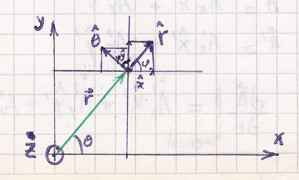
\includegraphics[scale=0.35]{images/fig_mc_polares_decomp.jpg}	
% 	\end{center}
% 	\caption{}
% \end{figure}
}
\[
	\hat{\varphi} = -\sin \varphi  \:\hat{x} + \cos  \varphi \:\hat{y}
\]
que lleva a 
\[
	\dtot{\hat{r}}{t} = - \sin \varphi \: \dot{ \varphi } \:\hat{x} + \cos \varphi \: \dot{ \varphi } \:\hat{y} =
	\dot{\vp} \: \hat{\vp}
\]
y entonces 
\[
	\dtot{\vb{x}}{t} = \dot{r} \:\hat{r } + r \:\dot{\vp} \: \hat{\vp} + \dot{z} \:\hat{z}.
\]

\notamargen{
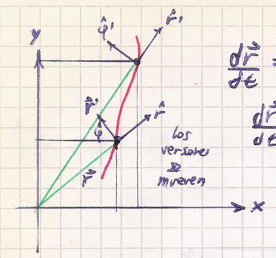
\includegraphics[scale=0.4]{images/fig_mc_polares_arbitrario.jpg}
}
% que se puede escribir como 
% \[
% 	\dtot{\vb{r}}{t} = \dot{r} \: \hat{r } + r \dot{\vp} \: \hat{\vp} = \dot{\vb{r}}
% \]
% y extraemos de conclusión que 
% \[
% 	\dtot{\hat{r}}{t} = \dot{\vp} \: \hat{\vp}
% \]

Para la aceleración hay que derivar la velocidad con respecto al tiempo
\[
	\ddot{\vb{x}} = \dtot{}{t} ( \dot{r} \: \hat{r} + r\dot{\vp} \: \hat{\vp} + \dot{z} \:\hat{z} ) 
\]
\[
	\ddot{\vb{x}} = \ddot{r} \:\hat{r} + \dot{r} \: \dtot{\hat{r}}{t} + \dot{r} \: \dot{\vp} \: \hat{\vp}
	+ r \left( \ddot{\vp} \: \phiver + \dot{\vp} \: \dtot{\hat{\vp}}{t} \right) + \ddot{z} \:\hat{z}
\]
y utilizando 
\[
	\dtot{\hat{\vp}}{t} = - \dot{ \vp } ( \cos \vp \:\hat{x} + \sin  \vp \:\hat{y} ) = - \dot{\vp} \: \hat{r}
\]
finalmente se arriba a
\[
	\ddot{\vb{x}} = ( \ddot{r} - r\dot{\vp}^2 ) \rver + ( r\ddot{\vp} + 2 \dot{r} \dot{\vp} ) \phiver + \ddot{z} \:\hat{z}.
\]

Para problemas de dos dimensiones suele utilizarse un sistema coordenado, conocido como coordenadas polares, que es el 
de cilíndricas con $ z \equiv 0 $. Las expresiones de velocidad y aceleración polares correspondientes serán las 
obtenidas en esta sección luego de {\it borrar} la coordenada $z$.

\subsection{Coordenadas esféricas}

Para el sistema esférico la deducción de la equivalencia cartesiana de los versores es un poco más trabajosa que en el 
sistema cilíndrico (donde en realidad estos versores viven en un plano $z$ cte.) y el álgebra implicado es algo 
engorroso. La expresión de los versores es
\[
	\rver = \cos\vp \sin\theta\xver + \sin\vp\sin\theta\yver + \cos\theta\zver,
\]
\[
	\phiver = -\sin\vp \xver + \cos\vp \yver,
\]
\[
	\thetaver = \cos\theta \cos\vp \xver + \cos\theta\sin\vp\yver - \sin\theta\zver.
\]
\notamargen{Dado que este es un curso básico pero que se jacata de visual, tendriamos que poner ilustraciones del 
carajo de los vectores en esféricas y cilíndricas para que quede intuitivo sus dificultades cuando el problema en
cuestión no tiene las simetrías explícitas de estos sistemas.}

Un vector de posición es simplemente
\[
	\vb{x} = r \rver
\]
aunque en el $\rver$ está {\it escondida} la dependencia angular. Consignaremos a continuación solamente las 
expresiones finales para la velocidad y aceleración, que son respectivamente
\[
	\vb{v} = \dot{\vb{x}} = \dot{r} \rver + r\dot{\theta}\thetaver + r\dot{\vp}\sin\theta\phiver
\]
\begin{multline*} % \vb no se da cuenta que multline ES modo matemático (por ello el .\ inicial)
	\!\: \vb{a} = \ddot{\vb{x}} = ( \ddot{r} - r\dot{\theta}^2 - r\dot{\vp}^2 \sin^2 \theta )\rver +
	( r\ddot{\theta} + 2\dot{r}\dot{\theta} - r\dot{\vp}^2 \sin \theta \cos\theta )\thetaver \: + \\
	( r \ddot{\vp}\sin\theta + 2 \: \dot{r} \: \dot{\vp} \sin\theta + 2 \: r \:\dot{\theta} \:\dot{\vp} \cos\theta )\phiver 
\end{multline*}
	

% =================================================================================================
\section{Transformación entre sistemas en rotación}
% =================================================================================================

Otro tipo de transformación común entre sistemas de coordenadas (en el plano) que comparten origen es la rotación.

Suponiendo un sistema de coordenadas $(x,y)$ fijo (que llamaremos ``inercial'') de origen $O$ y otro de coordenadas 
$(x',y')$, que está rotando en torno a ese origen (sistema ``móvil''), interesa ver qué consecuencias tiene sobre la 
velocidad y aceleración de un vector de posición \vb{A}, el hecho de determinarlas desde uno u otro sistema. Si bien 
hablamos de un sistema {\it fijo}, en realidad ambos se hallan en rotación entre sí. 

Como se ve en la FIGURA XXX 
\notamargen{
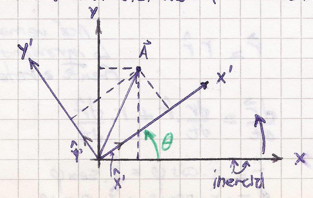
\includegraphics[scale=0.4]{images/fig_mc_sist_rotantes.jpg}
}
la posición instantánea entre sistemas está determinada por el ángulo $\theta(t)$ y, dado que ambos sistemas comparten 
el origen, los mismos son coincidentes en $\theta = 0$. 
% Como el sistema en rotación varía la posición de sus ejes con el tiempo, sus versores asociados $(\xver', \yver')$ 
% también variarán con el tiempo (pese a que son cartesianos).

Dado que los sistemas no se hallan entre sí a velocidad constante\footnote{Aún en el caso de $ \theta(t) = cte.$ la 
velocidad no es constante como vector puesto que cambia de dirección todo el tiempo.} es patente que las ecuaciones de 
Newton se verán modificadas.
Para un vector \vb{A} constante con respecto al sistema inercial, cualitativamente esperaríamos observarlo desde el 
sistema móvil en alguna suerte de movimiento dado por el efecto dinámico de la rotación\footnote{Si estoy montado en el 
caballo de madera de una calesita veré a mi abuela, que me espera inmóvil a un lado, como dotada de movimiento.}. Veamos 
qué surge de la cuenta algebraica.

El mismo vector de acuerdo a los dos sistemas de coordenadas en el plano, es
\[
	\vb{A}(t) = A_x\xver + A_y\yver         \qquad\qquad               \vb{A}'(t) = A_x'\xver' + A_y'\yver'
\]
donde las coordenadas primadas refieren al sistema móvil. Nótese que los versores asociados en ambos casos $(\xver, 
\yver)$ y $(\xver', \yver')$ son constantes, esto es, no dependen del tiempo. Que ambos sistemas se hallen en rotación 
entre sí no es intrínseco de alguno de ellos.
Un observador del sistema primado ve a sus ejes fijos mientras que en las medidas que realiza sobre \vb{A} verá una 
dinámica particular. 

Si consideramos la variación temporal de \vb{A}' pero como es vista desde el sistema inercial resulta 
\[
	\left. \dtot{\vb{A}}{t} \right|_\text{inercial} = 
	\dot{A_x'} \xver' + A_x'\dot{\xver'} + \dot{A_y'}\yver' + A_y' \dot{\yver'},
\]
porque para un observador en el sistema inercial se mueven las componentes del vector y los versores.

\notamargen{Esta notación es oscura, habría que ver una mejor manera de explicar esto.}

La variación temporal de los versores la conocemos porque es la misma situación geométrica que la encontrada para el 
caso de los versores cilíndricos $(\rver,\phiver)$. Podemos hallar la equivalencia
\[
	\dtot{\hat{x}'}{t} = \dot{\theta} \yver'         \qquad \qquad          \dtot{\hat{y}'}{t} = -\dot{\theta} \xver'.
\]

Desde el sistema móvil los versores son por supuesto constantes (el sistema móvil no es consciente de su movimiento) de 
modo que 
\[
	\left. \dtot{\vb{A}}{t} \right|_\text{móvil} = \dot{A_x'}\xver' + \dot{A_y'}\yver'
\]
y entonces
\[
	\left. \dtot{\vb{A}}{t} \right|_\text{fijo} = \left. \dtot{\vb{A}}{t} \right|_\text{móvil}
	+ A_x' \dot{\theta}\yver' - A_y'\dot{\theta}\xver'.
\]
% donde 
% \[
% 	\left. \dtot{\vb{A}'}{t} \right|_\text{móvil} \equiv \sum_i \dtot{A_i'}{t} \: \hat{e_i}'
% \]
% \[
% 	\left. \dtot{\vb{A}}{t} \right|_\text{móvil} = \dot{A_x'}\xver' + \dot{A_y'}\yver'
% \]

Si definimos
\[
	\vb{\omega} = \dot{\theta} \zver,
\]
entonces resulta que
\[
	\vb{\omega}\times\vb{A}' = \dot{\theta} \zver \times ({A_x'}\xver' + {A_y'}\yver') =
	A_x' \dot{\theta}\yver' - A_y'\dot{\theta}\xver'.
\]

Volviendo a la derivada de \vb{A} tenemos
\[
	\left. \dtot{\vb{A}}{t} \right|_\text{fijo} = \left. \dtot{\vb{A}}{t} \right|_\text{móvil}
	+ \vb{\omega} \times \vb{A}'
\]
que nos da la variación temporal de un vector \vb{A} visto desde un sistema fijo en términos de lo que se mediría
en un sistema (móvil) que está en rotación respecto al primero.

Si ahora la especializamos para un vector de posición \vb{x}, obtenemos la velocidad  
\[
	\left. \vb{v} \right|_\text{fijo} = \left. \vb{v} \right|_\text{móvil} + \vb{\omega} \times \vb{x}',
\]
donde 
\[
	\left. \vb{v} \right|_\text{móvil} = \dot{x}' \xver' + \dot{y}' \yver' 
\]

Asimismo, la aceleración se obtiene aplicando la relación al vector $\vb{v} \equiv d\vb{x}/dt$, de manera que 
tendremos
\[
	\left. \vb{a} \right|_\text{fijo} = \left. \dtot{\vb{v}}{t} \right|_\text{fijo} = \left. \dtot{\vb{v}}{t} \right|_\text{móvil} +
	\vb{\omega} \times \vb{v}'
\]
\[
	\left. \vb{a} \right|_\text{fijo} = 
	\dtot{}{t}\left[ \left. \dtot{\vb{x}}{t} \right|_\text{móvil} + \vb{\omega}\times\vb{x}' \right] +
	\vb{\omega} \times \left[ \left. \vb{v} \right|_\text{móvil} +	\vb{\omega}\times\vb{x}' \right]
\]

Ahora procedemos a trabajar las expresiones dentro del primer corchete, empezando por la derivada temporal de la velocidad
en el sistema móvil,
\[
	\left. \vb{a} \right|_\text{móvil} \equiv  
	\dtot{}{t}\left.( \dot{x}' \xver' + \dot{y}' \yver' )\right|_\text{móvil} = \ddot{x}' \xver' + \ddot{y}' \yver'
\]
y continuando con el término 
\[
	\left.\vb{\omega}\times\vb{x}'\right|_\text{móvil} = \omega x' \yver' - \omega y' \xver' ,
\]
cuya derivada es
\[
	\dtot{}{t}\left.\vb{\omega}\times\vb{x}\right|_\text{móvil} = 
	-( \dot{\omega} y' + \omega \dot{y}' )\xver' + ( \dot{\omega} x' + \omega \dot{x}' )\yver' =
	\left. \vb{\omega} \times\vb{v}'\right|_\text{móvil} + \left.\dot{\vb{\omega}} \times\vb{x}'\right|_\text{móvil}
\]

Juntando todo resulta
\[
	\left. \vb{a}\right|_\text{fijo} = \left. \vb{a}\right|_\text{móvil} 
	+ \left.\dot{\vb{\omega}} \times\vb{x}'\right|_\text{móvil} + 2 \:\vb{\omega}\times\vb{v'} + \vb{\omega}
	\times (\vb{\omega} \times \vb{x}')
\]
donde el tercero es la aceleración de Coriolis y el cuarto la aceleración centrípeta.

Las leyes de Newton observadas desde el sistema fijo serán 
% Llamando $ \alpha = \dot{\omega} = \dtot{\omega}{t}$ resulta 
\[
	\vb{F} = m\vb{a} = m \left. \vb{a}\right|_\text{móvil} + m \: \dot{ \vb{\omega} } \times \vb{r} + 4 \: m \: 
	\vb{\omega}\times\vb{v'} + m \: [  \vb{\omega} \times (\vb{\omega}\times\vb{r} )]
\]
que se pueden reacomodar como  
\[
	m \left. \vb{a}\right|_\text{fijo} = 
	\vb{F} - m \left. \vb{a}\right|_\text{móvil} - m \: \dot{\vb{\omega}} \times \vb{r} - 4 \: m \: \vb{\omega}\times\vb{v'} -
	m \: [\vb{\omega} \times(\vb{\omega}\times\vb{r})]
\]
donde ahora en el RHS tenemos la fuerza $\vb{F}$ que es la única que produce par de acción y reacción, y los términos de 
fuerza lineal, de Coriolis y centrífuga.

Si $\vb{\omega} = cte.$ entonces la fuerza lineal es nula.

\notamargen{Está un poco inconsistente la notación utilizada, con lo de móvil y la prima. La carpeta tiene muchos
typos. El 'Problema' de la hoja 5R no lo entiendo; en realidad parece estar vinculado a sólidos. Habría que decidir si 
ponerlo o no. En caso negativo, ¿qué otro se puede ubicar?}

\begin{notasfinales}

\label{nota_suma_ineqj}
\item{ \bf Sumatoria de torques}
Una manera de convencerse de que esta escritura es posible es hacer un diagrama de los diferentes términos que
aparecen en esta doble sumatoria. Es fácil de ver que con el añadido del término $\vb{x}_j \times \vb{F}_{ji} $ se está 
haciendo un doble conteo que justifica el $1/2$ que aparece luego.

Una demostración más matemática puede lograrse escribiendo la sumatoria $ j\neq i $ sin esta restricción, lo cual se 
puede hacer así:
\[
	\Sum{i=1}{N} \Sum{j\neq i}{N}  \vb{x}_i \times \vb{F}_{ij} = 
	\Sum{i=1}{N} \Sum{j=1}{N}  \vb{x}_i \times \vb{F}_{ij} ( 1 - \delta_{ij} )
\]
siendo $ \delta_{ij} $ la delta de Kronecker. Es claro que podemos hacer un cambio de etiquetas en las sumatorias 
puesto que los índices sumados son {\it mudos}, i.e.
\[
	\Sum{i=1}{N} \Sum{j=1}{N}  \vb{x}_i \times \vb{F}_{ij} ( 1 - \delta_{ij} ) = 
	\Sum{j=1}{N} \Sum{i=1}{N}  \vb{x}_j \times \vb{F}_{ji} ( 1 - \delta_{ij} )
\]
y dado que el orden de las sumatorias es irrelevante llegamos a
\[
	\Sum{i=1}{N} \Sum{j\neq i}{N}  \vb{x}_i \times \vb{F}_{ij} = \frac{1}{2}
	\Sum{i=1}{N} \Sum{j=1}{N} \left[ \vb{x}_i \times \vb{F}_{ij} ( 1 - \delta_{ij} ) +
	\vb{x}_j \times \vb{F}_{ji} ( 1 - \delta_{ij} )
	\right] 
\]

Regresando ahora a las sumatoria restringida obtenemos 
\[
	\Sum{i=1}{N} \Sum{j\neq i}{N}  \vb{x}_i \times \vb{F}_{ij} = \frac{1}{2}
	\Sum{i=1}{N} \Sum{j \neq i }{N} \left[ \vb{x}_i \times \vb{F}_{ij} + \vb{x}_j \times \vb{F}_{ji} \right] 
\]
que es el resultado buscado.


\end{notasfinales}


% ============================================================================

% \bibliographystyle{CBFT-apa-good} % (uses file "apa-good.bst")
% \bibliography{CBFT.Referencias} % La base de datos bibliográfica


\end{document}

	
		\documentclass[10pt,oneside]{CBFT_book}
	
	% Algunos paquetes
	
	\usepackage{amssymb}
	\usepackage{amsmath}
	\usepackage{graphicx}
	\usepackage{libertine}
	\usepackage{lipsum}
	\usepackage[numbers]{natbib}
	\setcitestyle{square}


	\usepackage{polyglossia}
	\setdefaultlanguage{spanish}

	\usepackage{CBFT.estilo} % Cargo la hoja de estilo
	
	% Tipografías
	% \setromanfont[Mapping=tex-text]{Linux Libertine O}
	% \setsansfont[Mapping=tex-text]{DejaVu Sans}
	% \setmonofont[Mapping=tex-text]{DejaVu Sans Mono}

	%===================================================================
	%	DOCUMENTO PROPIAMENTE DICHO
	%===================================================================

% \title{CBFT Mecánica clásica}
% \author{Mecánica lagrangiana}
% \date{\today}

\begin{document}
% \maketitle
% \tableofcontents
\chapter{Mecánica lagrangiana}

% =================================================================================================
\section{Principio de los trabajos virtuales}\index{Trabajos virtuales, principio de}
% =================================================================================================
\notamargen{Esto es sumamente sketchi, debemos leer la carpeta de la cursada y luego la
teoría.}

En las ecuaciones de Newton para un sistema de $N$ partículas, con $3N$ coordenadas,
\[
	m_i \vb{a}_i = \vb{F}_i,
\]
se pueden separar las fuerzas que actúan sobre cada partícula en fuerzas externas aplicadas $ \vb{F}_i^a $
y fuerzas de vínculo $ \vb{F}_i^v $. Es decir,
\[
	m_i \vb{a}_i = \vb{F}_i^a + \vb{F}_i^v,
\]
% dan cuenta de que sobre cada partícula actúan, en principio, fuerzas externas aplicadas $ \vb{F}_i^a $
% y fuerzas de vínculo $ \vb{F}_i^v $. 
o bien, expresando la aceleración en función de la derivada temporal del momento, 
%$ \dot{\vb{p}}_i = m_i \vb{a}_i$ 
resulta 
\[
	\dot{\vb{p}}_i - \vb{F}_i^a - \vb{F}_i^v = 0,
\]
y entonces, multiplicando cada término por un desplazamiento, en principio independiente, $ \delta\vb{x}_i $ y sumando se tiene
\[
	\sum_i^N \left( \dot{\vb{p}}_i - \vb{F}_i^a - \vb{F}_i^v \right) \cdot \delta\vb{x}_i  = 0.
\]
Nótese que esta ecuación es válida por serlo para cada partícula $i$.

\notamargen{Explicar qué es este principio y qué es un desplazamiento virtual.}
Supongamos ahora que estos desplazamientos son {\it compatibles} con los vínculos. Entonces
\[
	\sum_i^N \left( \dot{\vb{p}}_i - \vb{F}_i^a \right) \cdot \delta\vb{x}_i 
	- \sum_i^N  \vb{F}_i^v  \cdot \delta\vb{x}_i  = 0
\]
pero el segundo término es nulo porque los $ \delta\vb{x}_i $ son compatibles con los vínculos y como sabemos 
\notamargen{Hay que dejar bien el claro el asunto de que las fuerzas de vínculos son siempre perp a los desplazamientos
virtuales y que estos, ¿no son independientes?}
$ \vb{F}_i^v \perp \delta\vb{x}_i $.

Entonces
\be
	\sum_i^N \left( \dot{\vb{p}}_i - \vb{F}_i^a \right) \cdot \delta\vb{x}_i = 0,
% 	- \sum_i^N  \vb{F}_i^v  \cdot \delta\vb{x}_i  = 0
	\label{principio_virtual_work}
\ee
donde no se verifica, en general, que el primer vector en cada producto escalar sea nulo.

\textcolor{red}{
La expresión \eqref{principio_virtual_work} es el llamado {\it Principio de los Trabajos Virtuales},
y dada la independencia admitida en los desplazamientos virtuales $ \delta \vb{x}_i $, se sigue que la
sumatoria en \eqref{principio_virtual_work} es nula porque cada término es nulo, es decir
\[
	\dot{\vb{p}}_i - \vb{F}_i^a = 0 \quad \forall i
\]
}

\begin{ejemplo}{\bf Ejemplo de los bloques}

Para el ejemplo de los bloques
\[
	( m_1 \ddot{x}_1 - 2T )\delta x_1 + ( m_2 \ddot{x}_2 - m_2 g + T) \delta x_2 = 0
\]
pero en realidad $\delta x_1, \delta x_2$ no son independientes, están relacionados según $2\delta x_1 = \delta x_2$.
Entonces
\[
	( m_1 \ddot{x}_1 + 2 m_2 \ddot{x}_2 - 2 m_2 g )\delta x_1 = 0
\]
donde ahora $\delta x_1$ es compatible con los vínculos pero es independiente y arbitrario para el problema.
Entonces la ecuación anterior debe ser nula porque el paréntesis es nulo,
\[
	m_1 \ddot{x}_1 + 2 m_2 \ddot{x}_2 - 2 m_2 g = m_1 \ddot{x}_1 + 4 m_2 \ddot{x}_1 - 2 m_2 g = 0
\]
y de la última 
\[
	\ddot{x}_1 = \frac{2 m_2 g}{ (m_1 + 4m_2 ) }.
\]

Hemos llegado a la resolución en forma independiente de los vínculos.
\end{ejemplo}

\begin{ejemplo}{Más de un grado de libertad}

Si tenemos más de un grado de libertad, como en el caso de dos poleas sin masa.

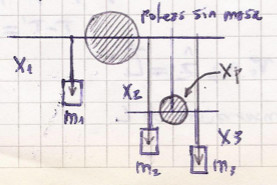
\includegraphics[scale=0.4]{images/fig_mc_dos_poleas.jpg}

Se tienen dos ecuaciones de vínculo
\[
	x_1 + x_p = \ell_1 \qquad \qquad (x_2 -x_p)+(x_3 -x_p) = \ell_2.
\]

El problema tiene cuatro coordenadas y dos ecuaciones de vínculo, lo cual nos deja dos grados de libertad.
La primer ecuación de vínculo permite liberarnos de $x_p$ y quedarnos en principio con los movimientos de
las tres masas. Entonces, ¿el principio de los trabajos virtuales? sería en este caso 
\[
	( m_1 \ddot{x}_1 - m_1 g )\delta x_1 + ( m_2 \ddot{x}_2 - m_2 g )\delta x_2 + ( m_3 \ddot{x}_3 - m_3 g )\delta x_3 = 0
\]
y luego podemos utilizar la segunda ecuación de vínculo, combinándola con la primera para llegar a 
\[
	x_2 + x_3 + 2x_1 = \text{ cte. }
\]
lo cual conduce a la relación 
\[
	\delta x_1 = -\frac{ \delta x_2 + \delta x_3 }{2}.
\]
Finalmente
\[
	( m_2 \ddot{x}_2 - m_2 g -\frac{m_1}{2} \ddot{x}_1 + \frac{m_1}{2} g ) \delta x_2 + 
	( m_3 \ddot{x}_3 - m_3 g -\frac{m_1}{2} \ddot{x}_1 + \frac{m_1}{2} g ) \delta x_3 = 0.
\]
\end{ejemplo}

\begin{notas}{Relación vínculos y desplazamientos:}
El hecho de que la fuerza de vínculo sea perpendicular a los desplazamientos puede
verse a partir de que la ecuación de vínculo en un sistema toma la forma
\notamargen{¿Y esta magia? Hay que aclarar realmente que sea así como se dice que es.}
\[
	f(\vb{x}_i) - K = 0 
\]
luego, derivando implícitamante cada ecuación y sumando (si se nos permite un pequeño
abuso de notación)
\[
	\sum_i^N \dpar{f}{\vb{x}_i} d\vb{x}_i = 0 
\]
pero esto no es otra cosa que
\[
	\nabla f \cdot \vb{\delta x} = 0
\]
donde debemos entender al gradiente y al vector $\vb{\delta x}$ como $N$ dimensionales.
\end{notas}


\subsection{Comentario vínculos}
\notamargen{Esto hay que consolidarlo todo. Volará.}
El trabajo de la fuerza de vínculos es nulo si el desplazamiento es virtual.
\[
	f(x_1,x_2,...,x_N,t) = 0
\]
\[
	\dpar{f}{x_1}\delta x_1 + ... +  \dpar{f}{x_N}\delta x_N = 0
\]
Como es un desplazamiento virtual, el tiempo $t$ está fijo (imagen fija = tiempo congelado)


% =================================================================================================
\section{Construcción del lagrangiano}
% =================================================================================================

Vamos a utilizar el principio de los trabajos virtuales para escribir las ecuaciones de la mecánica
de otra manera [¿?] sin preocuparnos por las fuerzas de vínculo, que en general pueden no ser 
conocidas o tener una naturaleza compleja.
\notamargen{Esta es la papa: las fuerzas de vínculo son difíciles de escribir si es esto posible 
del todo.}
Consideremos un sistema de $N$ partículas y $k$ ecuaciones de vínculo 
\begin{eqnarray*}
	& f_1(\vb{x}_1, \vb{x}_2,...,\vb{x}_n,t) = K_1  \\ 
	& ... ... ... \\
	& f_k(\vb{x}_1, \vb{x}_2,...,\vb{x}_n,t) = K_k 
\end{eqnarray*}
y por ende $3N-k$ grados de libertad (suponiendo que nos hallamos en 3 dimensiones).

Tenemos $N$ relaciones del tipo 
\be
	\vb{x}_i = \vb{x}_i(q_1,q_2,...,q_{3N-k},t)
	\label{x_part}
\ee
que significa que la posición de la partícula $i$-ésima depende en principio de las $3N-k$ coordenadas
generalizadas y del tiempo. Una variación de la misma tendrá la forma
\[
	\delta \vb{x}_i =  \sum_{j=1}^{3N-k} \left( \dpar{\vb{x}_i}{q_j} \right) \delta q_j + 
	\dpar{\vb{x}_i}{t}\delta t
\]
y suponiéndola un desplazamiento virtual el último término se anula puesto que $\delta t=0$ en ese
caso y entonces
\be
	\delta \vb{x}_i =  \sum_{j=1}^{3N-k} \left( \dpar{\vb{x}_i}{q_j} \right) \delta q_j.
	\label{delta_x_to_delta_q}
\ee

Por otro lado, del principio de los trabajos virtuales \eqref{principio_virtual_work} es
\[
	\sum_i^N \dot{\vb{p}}_i \cdot \delta \vb{x}_i - \sum_i^N  \vb{F}_i^a \cdot \delta \vb{x}_i = 0,
\]
donde $\vb{F}_i^a$ es la fuerza aplicada externa que no incluye las fuerzas de vínculo. El primer término 
se puede reescribir como
\[
	\dot{\vb{p}}_i \cdot \delta \vb{x}_i = m_i \dtot{\vb{v}_i}{t} \cdot \sum_{j=1}^{3N-k} 
	\left( \dpar{\vb{x}_i}{q_j} \right) \delta q_j,
\]
resultando
\be
	\sum_i^N m_i \dtot{\vb{v}_i}{t} \cdot \sum_{j=1}^{3N-k} \left( \dpar{\vb{x}_i}{q_j} \right)
	\delta q_j - \sum_i^N  \vb{F}_i^a \cdot \delta \vb{x}_i = 0
	\label{virtual_work_2}
\ee
Se ha pasado de una descripción en términos de $\delta \vb{x}_i$ ($3N$ variables) a otra en términos de $\delta q_j$
($3N-k$ coordenadas generalizadas).

La idea ahora es reescribir todo en términos más convenientes, para que aparezca un término multiplicado
a una variación arbitraria. De esta manera quedará una sumatoria de un sumando multiplicado por una
variación igualada a cero. No cabe otra posibilidad que el sumando sea nulo para cada índice de la suma.
\notamargen{Escrito muy mal este texto. La idea es clara, no obstante: hay que purificarla}

Consideremos en primer lugar la derivada total del producto siguiente
\[
	\frac{d}{dt}\left( m_i\vb{v}_i \cdot \dpar{\vb{x}_i}{q_j} \right) =
	m_i \dtot{\vb{v}_i}{t} \cdot \dpar{\vb{x}_i}{q_j} + m_i \vb{v}_i 
	\cdot \frac{d}{dt}\left(\dpar{\vb{x}_i}{q_j}\right),
\]
y en segundo lugar la velocidad de cada partícula, que proviene de la derivada total de cada ecuación 
\eqref{x_part} y resulta
% )Pero la diferencial del vector $\vb{x}_i$ es (notemos que no es una variación)
% \[
% 	d\vb{x}_i = \sum_{j=1}^{3N-k} \left( \dpar{\vb{x}_i}{q_j} \right) dq_j + \dpar{\vb{x}_i}{t} dt
% \]
% y entonces
\[
	\vb{v}_i = \dtot{\vb{x}_i}{t} = \sum_{j=1}^{3N-k} \left( \dpar{\vb{x}_i}{q_j} \right)
	\dot{q}_j + \dpar{\vb{x}_i}{t}.
\]

A partir de esta última es claro ver que la derivada de la velocidad de la partícula $i$-ésima respecto a la coordenada 
$l$-ésima es
\be
	\dpar{\vb{v}_i}{\dot{q}_l} = \dpar{\vb{x}_i}{q_l}.
	\label{relacion_derivadas}
\ee
\notamargen{Una manera menmotécnica de recordar esto es con el siguiente esquema:
\[
	\dpar{\vb{v}_i}{\dot{q}_l} = \frac{\partial \vb{x}_i/\partial t}{\partial q_l/\partial t} =
	\dpar{\vb{x}_i}{q_l}.
\]
}
La ecuación de la velocidad se puede derivar otra vez, con respecto a $q_l$, obteniéndose
\[
	\dpar{\vb{v}_i}{q_l} = \frac{\partial}{\partial q_l} \left( \dtot{\vb{x}_i}{t} \right) =
	\sum_{j=1}^{3N-k} \dparcru{\vb{x}_i}{q_j}{q_l} \dot{q}_j + 
	\dparcru{\vb{x}_i}{t}{q_l},
\]
y se puede ver que invirtiendo el orden de derivación, esto significa que 
\[
	\dpar{\vb{v}_i}{q_l} = \frac{d}{dt} \left( \dpar{\vb{x}_i}{q_l} \right).
\]

\notamargen{El hecho de que se pueda sacar fuera la derivada temporal y pasar adentro la derivada
con respecto a la coordenada generalizada $q$ puede verse haciendo la cuenta de manera explícita.}
% 
% \[
% 	\frac{d}{dt} \left( \dpar{\vb{x}_i}{q_l} \right) = 
% 	\frac{d}{dt} \left( \sum_{j=1}^{3N-k} \dparcru{\vb{x}_i}{q_j}{q_l} dq_j +
% 	\dparcru{\vb{x}_i}{t}{q_l} dt \right) 
% \]
% de tal manera que 
% \[
% 	\frac{d}{dt} \left( \dpar{\vb{x}_i}{q_l} \right) = \dpar{\vb{v}_i}{q_l}
% \]

Volviendo ahora a \eqref{virtual_work_2} y usando los resultados recientes tenemos
\[
	\sum_i^N \sum_{j=1}^{3N-k} 
	\left[ \frac{d}{dt} \left( m_i \vb{v}_i \dpar{\vb{x}_i}{q_j} \right) - 
	m_i \vb{v}_i \frac{d}{dt}\left( \dpar{\vb{x}_i}{q_j} \right) \right] \delta q_j
	- \sum_i^N  \vb{F}_i^a \cdot \delta \vb{x}_i = 0
\]
donde modificaremos el corchete expresando derivadas con respecto a la posición $\vb{x}$ en términos
de derivadas con respecto a la velocidad $\vb{v}$, de manera que 
\[
	\left[ \frac{d}{dt} \left( m_i \vb{v}_i \dpar{\vb{v}_i}{\dot{q}_j} \right) -
	m_i \vb{v}_i \dpar{\vb{v}_i}{q_j} \right]
\]
y usando el {\it trick} usual
\[
	\vb{v} \dpar{\vb{v}}{q} = \frac{1}{2} \dpar{ \vb{v}^2 }{q} 
\]
resulta
\[
	\left\{ 
	\frac{d}{dt} \left[ \frac{\partial}{\partial \dot{q}_j} \left( \frac{m_i}{2} \vb{v}_i^2 \right) \right] - 
	\frac{\partial}{\partial q_j} \left( \frac{m_i}{2} \vb{v}_i^2 \right) \right\}
\]

Es hora ya de introducir la sumatoria en $i$ hacia el interior del corchete, y la ecuación original es ahora 
\[
	\sum_{j=1}^{3N-k} \left\{ 
	\frac{d}{dt} \left[ \frac{\partial}{\partial \dot{q}_j}
	\left( \sum_i^N \frac{m_i}{2} \vb{v}_i^2 \right) \right] 
	- \frac{\partial}{\partial q_j} \left( \sum_i^N \frac{m_i}{2} \vb{v}_i^2 \right) \right\} \delta q_j
	- \sum_i^N  \vb{F}_i^a \cdot \delta \vb{x}_i = 0
\]
y dentro de los paréntesis ha aparecido la energía cinética $T$. La sumatoria en $j$ no era otra cosa que la suma 
de las derivadas de los momentos, y entonces
\[
	\sum_i^N \dot{\vb{p}}_i \cdot \delta \vb{x}_i =
	\sum_{j=1}^{3N-k} \left\{ \frac{d}{dt} \left[ \frac{\partial T}{\partial \dot{q}_j} \right] -
	\frac{\partial T}{\partial q_j} \right\} \delta q_j = \sum_i^N  \vb{F}_i^a \cdot \delta \vb{x}_i.
\]

Escribiendo la variación $\delta\vb{x}$ en términos de $\delta q$ a través de \eqref{delta_x_to_delta_q}
% \[
% 	\delta\vb{x}_i = \sum_{j=1}^{3N-k} \dpar{\vb{x}_i}{q_j}\delta q_j
% \]
se llega a 
\[
	\sum_{j=1}^{3N-k} \sum_i^N \left( \vb{F}_i^a \cdot \dpar{\vb{x}_i}{q_j} \right) \: \delta q_j =  
	\sum_{j=1}^{3N-k} Q_j \: \delta q_j
\]
siendo 
\[
	Q_j = \sum_i^N \left( \vb{F}_i^a \cdot \dpar{\vb{x}_i}{q_j} \right)
\]
la fuerza generalizada en el grado de libertad $j$. Entonces
\be
	\sum_{j=1}^{3N-k} \left\{ \frac{d}{dt}
	\left[ \frac{\partial T}{\partial \dot{q}_j} \right] - \frac{\partial T}{\partial q_j} - Q_j \right\} \delta q_j =  0
	\label{eq_el_0}
\ee
% y dado que las variaciones $\delta q_j$ son independientes se sigue que 

Si suponemos que las fuerzas son conservativas, provienen de un potencial, entonces 
\[
	\vb{F}_i^a = -\dpar{V(\{ \vb{x}_j \})}{\vb{x}_i}
\]
y expresando la fuerza $Q_j$ en términos del potencial $V$
\[
	Q_j = \sum_i^N \vb{F}_i^a \cdot \dpar{\vb{x}_i}{q_j} = 
	- \sum_i^N \dpar{V}{\vb{x}_i} \cdot \dpar{\vb{x}_i}{q_j} = -\dpar{V}{q_j},
\]
el cual, insertado en la ecuación \eqref{eq_el_0}, conduce a
\[
	\sum_{j=1}^{3N-k} \left\{ \frac{d}{dt}
	\left[ \frac{\partial T}{\partial \dot{q}_j} \right] - \frac{\partial}{\partial q_j} \left( T - V \right) \right\} \delta q_j =  0.
\]
% \[
% 	Q_j \: \delta q_j = -\dpar{V}{q_j} \: \delta q_j
% \]
% y como $V=V(\vb{x}_1,...,\vb{x}_n)$ se tiene 
% \[
% 	V = \sum_i^N  \dpar{V}{r_i} \delta \vb{x}_i = \dpar{V}{\vb{x}_i} \cdot \dpar{\vb{x}_i}{q_j} \delta q_j =
% \]
% pero 
% \[
% 	Q_j = - \dpar{V}{q_j}
% \]
% y entonces 
% \[
% 	\sum_{j=1}^{3N-k} \left\{ 
% 	\frac{d}{dt} \left( \dpar{T}{\dot{q}_j} \right) - \frac{\partial}{\partial q_j}
% 	\left( T - V \right) \right\} \delta q_j =  0.
% \]
Dado que $ V = V(\vb{x}_1,...,\vb{x}_N) = V( \{ q_j \} )$ (no depende de las velocidades generalizadas $ \dot{q}_j $) se puede escribir 
\[
	\sum_{j=1}^{3N-k} \left\{ \frac{d}{dt}
	\left[ \frac{\partial}{\partial \dot{q}_j} \left( T - V \right) \right] - 
	\frac{\partial}{\partial q_j} \left( T - V \right) \right\} \delta q_j =  0.
\]
y definiendo al lagrangiano\index{Lagrangiano} $\Lag$ como 
\[
	\Lag \equiv T - V
\]
se arriba a
\[
	\sum_{j=1}^{3N-k} \left[
	\frac{d}{dt} \left( \dpar{\Lag}{\dot{q}_j} \right) -  \dpar{\Lag}{q_j} \right] \delta q_j =  0.
\]
Nótese que $\Lag = \Lag( q_1,...,q_{3N-k}, \dot{q}_1, ..., \dot{q}_{3N-k}, t ) $, es decir que es función 
del conjunto $(\{ q_j \}, \{ \dot{q}_j \}, t)$. De esta manera las ecuaciones resultantes serán, a lo sumo,
ecuaciones diferenciales para $q_j(t)$ de orden dos.

Si existieran fuerzas aplicadas que no provienen de un potencial (no conservativas) entonces
\[
	Q_j + Q_j^{NC} = -\dpar{V}{q_j} + Q_j^{NC},
\]
y las ecuaciones adquieren un término extra 
\[
	\sum_{j=1}^{3N-k} \left[
	\frac{d}{dt} \left( \dpar{\Lag}{\dot{q}_j} \right) - \dpar{\Lag}{q_j} - Q_j^{NC} \right] \delta q_j = 0.
\]

Como esto vale para todo grado de libertad $j$, puesto que las variaciones son independientes, llegamos a
\[
	\frac{d}{dt} \left( \dpar{\Lag}{\dot{q}_j} \right) -  \dpar{\Lag}{q_j} = Q_j^{NC}
\]
que son las ecuaciones de Euler-Lagrange con presencia de fuerzas no conservativas. 
Este es el resultado más importante del capítulo.
\notamargen{No sé si es la primera vez que aparecen. De serlo habría que remarcarlo como es debido, tal vez
recuadrar}

Se tienen así una formulación para los problemas mecánicos en términos de ecuaciones diferenciales para los
grados de libertad $q_j$ que prescinden del conocimiento de las fuerzas de vínculo.

\subsection{Algunos ejemplos del lagrangiano}

% ~~~~~~~~~~~~~~~~~~~~~~~~~~~~~~~~~~~~~~~~~~~~~~~~~~~~~~~~~~~~~~~~~~~~~~

\begin{ejemplo}{\bfseries Bloques deslizantes}

Teníamos el vínculo 
\[
	-2x_1 + x_2 = \text{ cte. }
\]
Luego,
\[
	T = \frac 1 2 m_1 \dot{x}_1^2 + \frac 1 2 m_2 \dot{x}_2^2 \qquad \qquad V = -m_2 g x_2
\]
y tomando $x_2$ como independiente llego a
\[
	T-V = \frac{1}{2}\left( \frac{m_1}{4} + m_2 \right) \dot{x}_2^2 + m_2gx_2.
\]
Luego, las ecuaciones de E-L serán
\[
	\dtot{}{t}\left( \dpar{\Lag}{\dot{x}_2} \right) - \dpar{\Lag}{x_2} =
	\left( \frac{m_1}{4} + m_2 \right) \ddot{x}_2 - m_2 g = 0
\]
que conduce a 
\[
	\ddot{x}_2 = \frac{m_2 g}{\frac{m_1}{4} + m_2 },
\]
que es a lo que se tenía que llegar.
\end{ejemplo}

\begin{ejemplo}{\bfseries Péndulo}

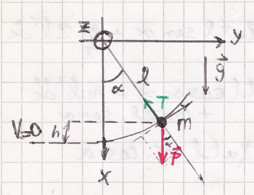
\includegraphics[scale=0.35]{images/fig_mc_pendulo_lag.jpg}

Las ecuaciones son 
\[
	m\ell \dot{\alpha}^2 = - T + m g \cos \alpha \qquad 
	m\ell \ddot{\alpha} = - m g \sin \alpha
\]
y se podría resolver desde aquí nomás. Pero escribamos el lagrangiano
\[
	\Lag = T-V = \frac 1 2 m \ell^2 \dot{\alpha}^2 - mg\ell(1-\cos \alpha)
\]
Sus ecuaciones de E-L son
\[
	m \ell \ddot{\alpha} + mg\ell \sin \alpha = 0
\]
que es la ecuación del péndulo $\ddot{\alpha} = -g/\ell \sin \alpha$.

\end{ejemplo}

\begin{ejemplo}{\bfseries Aro acelerado }

\notamargen{Falta ilustración del aro y sistema coordenado.}
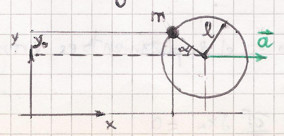
\includegraphics[scale=0.35]{images/fig_mc_aro_acelerado_lag.jpg}

Supongamos un aro horizontal en una mesa sin rozamiento. Tiene un único grado de libertad.

El vínculo es
\[
	(x - \nicefrac{1}{2} \: at^2)^2 + (y-y_0 )^2 = \ell^2
\]
y las posiciones instantáneas de la masa $ m $
\[
	x = \frac{1}{2}at^2 - \ell \cos(\vp) \qquad  y = y_0 + \ell \sin(\vp)
\]

Es conveniente utilizar el ángulo $\vp$ como coordenada generalizada. Pero $\vp$ está solidaria al aro.
Eso no es un problema siempre que el $\Lag$ esté medido en un sistema inercial.

En este caso no hay potencial pero como $\vp$ es una coordenada vista en un sistema no inercial, aparecerán
las fuerzas ficticias asociadas al movimiento.
Serán
\[
	\dot{x} = at + \ell \sin(\vp) \dot{\vp} \qquad \dot{y} = \ell \cos(\vp) \dot{\vp}
\]
\notamargen{La $T$ del $\Lag$ es la vistda desde un sistema INERCIAL siempre; en todo caso luego aparecen
las fuerzas ficticias necesarias. ESTO HAY QUE ESTUDIARLO Y ENTENDERLO.
}
y luego 
\[
	\Lag = T = \frac{1}{2} m (\dot{x}^2 + \dot{y}^2 ) = \frac{1}{2} m
	(a^2 t^2 + 2at\ell\sin(\vp)\dot{\vp}+\ell^2\dot{\vp}^2)
\]

Las ecuaciones de Euler-Lagrange serán 
\[
	\dtot{}{t}\left( \dpar{\Lag}{\dot{\vp}}\right) - \dpar{\Lag}{\vp} = 
	m \ell^2 \ddot{\vp} + ma\ell \sin(\vp) = 0
\]
lo cual resulta en la ecuación de movimiento
\notamargen{El lagrangiano se dedujo de las ecuaciones de Newton, entonces debemos calcular $T,V$ de un sistema
inercial. Acá no se entiende si lo que se hace en la carpeta está bien o no, en el sentido de que parece que al
usar una coordenada que no es inercial estamos calculando T no inercial.? }
\[
	\ddot{\vp} = - \frac{a}{\ell} \sin(\vp) 
\]
que es una ecuación que da oscilaciones, como la de un péndulo. Estas oscilaciones están causadas, claramente,
por la aceleración $a$.

En este ejemplo se ve que se calcula la energía cinética $T$ en un sistema inercial; no obstante, este valor está
expresado en términos de una coordenada que no es inercial (es solidaria al aro). Aparecen entonces las fuerzas 
inerciales que tienen que aparecer y punto.
\end{ejemplo}
% ~~~~~~~~~~~~~~~~~~~~~~~~~~~~~~~~~~~~~~~~~~~~~~~~~~~~~~~~~~~~~~~~~~~~~~

\begin{ejemplo}{\bf Problema 5 --para vínculos--}

Este problema es de vínculos y trabajos virtuales. Habría que reubicarlo.

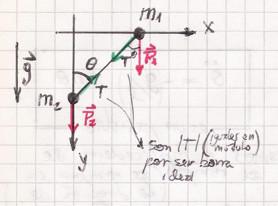
\includegraphics[scale=0.35]{images/fig_mc_oscilador_barra.jpg}

Se tienen dos masas $m_1$ y $m_2$ de manera que en principio se tendrían seis coordenadas; no obstante como el movimiento
es en un plano (se puede tomar el $z=0$ como tal) y las masas están restringidas a moverse a lo largo del eje que las
engarza se tiene, adoptando el esquema de la figura,
\[
	z_1 = z_2 = 0 \qquad \qquad x_2 = y_1 = 0
\]
es decir cuatro ecuaciones de vínculo a la cual le sumamos una quinta
\be
	x_1^2 + y_2^2 = \ell^2
	\label{vinculo_problema_5}
\ee
de manera que resulta un problema para un único grado de libertad. Obviando los subíndices que no son necesarios, y diferenciando
implícitamente la ecuación \eqref{vinculo_problema_5} se obtiene 
\[
	x dx + y dy = 0 
\]
Utilizando el ángulo $\theta$ y parametrizando las variables implicadas en \eqref{vinculo_problema_5} de acuerdo con 
\[
	x = \ell \sin \theta \qquad y = \ell \cos \theta
\]
vemos que es una buena coordenada porque verifica el vínculo de manera natural.

Planteando las ecuaciones 
\[
	( T \sin \theta - m_1 \ddot{x} ) \delta x + ( m_2 g - T \cos \theta - m_2 \ddot{y} ) \delta y = 0
\]
\be
	x \delta x = -y \delta y
	\label{relacion_deltas}
\ee
pero usando la última, se tiene
\[
	-\frac{x}{\ell}T\delta x - \frac{y}{\ell}T\delta y = 0 
\]
de manera que desaparece la tensión. Entonces
\[
	m_2 \ddot{x} \delta x = m_2 (g - \ddot{y}) \delta y
\]
que es una ecuación de Lagrange de primera especie. Usando otra vez \eqref{relacion_deltas}
\[
	- m_1 \ddot{x} \frac y x = m_2 (g - \ddot{y})
\]
y entonces ahora habría que convertir a expresar todo en términos de $\theta$. Derivando las expresiones de $x,y$ en términos
del ángulo $\theta$ resulta que 
\[
	-m_1 \ell ( \ddot{\theta} \cos \theta - \dot{\theta}^2 \sin \theta ) \frac{\cos \theta}{\sin \theta}  = 
	m_2 ( g + \ell \ddot{\theta} \sin \theta + \ell \dot{\theta} \cos \theta )
\]
\[
	\ddot{ \theta } \ell ( m_2 \sin \theta + m_1 \frac{\cos^2 \theta}{\sin \theta} ) + 
	\dot{\theta}^2 \ell (m_2 \sin \theta - m_1 \cos \theta ) + m_2 g = 0
\]
Si $ m_1 = m_2 $ entonces
\[
	\ddot{ \theta } \ell \frac{m}{\sin \theta} + m  g = 0 
\]
\[
	\ddot{ \theta } = -\frac{ g }{ \ell } \sin \theta,
\]
y vemos que es un péndulo.

Ahora se quisiera calcular la tensión $T$. Se utilizarán multiplicadores de Lagrange. Sea que los vínculos se rompen (se rompen, por supuesto, en la 
dirección de las fuerzas de vínculos). Supongamos que existe $y_1$ (hay desplazamiento en la coordenada $y_1$) entonces existirá $\lambda$ tal que 
$\lambda  \delta y_1 \neq 0$
\[
	\delta y_1 ( m_1 \ddot{y}_1 - \lambda - m_1 g ) \qquad \lambda = m_1 g
\]
pero la ecuación en (1) (página anterior) debe seguir valiendo.
\[
	\lambda_T + x \delta x + \lambda_T y \delta y 
\]
\[
	( m_1 \ddot{x} + \lambda_T x ) \dx + ( m_2 (g - \ddot{y} ) + \lambda_T + y ) \dy = 0
\]
lo cual vale si $\lambda_T = - \frac T \ell $.
Y se ve que el multiplicador de Lagrange es la tensión (vínculo) -- la fuerza asociada a que se cumpla el vínculo --.
Tengo un multiplicador por cada vínculo. Si hay $n$ vínculos y quiero un vínculo uso un solo multiplicador.
Pero ahora $\dx$ y $\dy$ son independientes, entonces deben anularse por separado los dos miembros de la ecuación de Newton.
\[
	m_1 \ddot{x} + \lambda_T x  \qquad \qquad m_ 2(g -\ddot{y}) + \lambda_T y
\]
\[
	\lambda_T = - \frac{m_1 \ddot{x}}{x} 
\]
\[
	\lambda_T = -\frac{ m_1 ( \ddot{ \theta } \cos \theta - \dot{\theta}^2 \sin \theta ) }{\sin \theta} =
	m_1 (\frac g \ell \cos \theta - \dot{\theta}^2 )
\]
\end{ejemplo}



% =================================================================================================
\section{Invariancia del lagrangiano ante adición de una derivada total}
% =================================================================================================

En los ejemplos del péndulo y del aro acelerado [CITAR], la resolución del sistema a través de las ecuaciones de 
Euler-Lagrange condujo a las mismas ecuaciones de movimiento (lo que signfica que, para iguales condiciones iniciales, 
la física del sistema es la misma) pero se partió de dos lagrangianos diferentes
\[
	\Lag = \frac 1 2 m \ell^2 \dot{\alpha}^2 + m g \ell \cos \alpha \qquad
	\Lag'= \frac 1 2 m \left( \ell^2 \ddot{\alpha} + 2 \ell g t \sin \alpha \: \dot{\alpha} + g^2 t^2 \right)
\]
\notamargen{La aceleración del aro era $a$ pero escribimos $g$ para enfatizar que tienen la misma forma.}
que llevaban a
\[
	\ell \ddot{\alpha} + g \sin \alpha = 0. 
\]
Es decir, que desde el punto de vista del movimiento del sistema, los dos lagrangianos son equivalentes.
Pero notemos que el término central en $\Lag'$ aparece vinculado a 
\[
	\dtot{}{t}\left( m l g t \cos \alpha \right) = -m \ell g t \dot{\alpha} \sin \alpha + m l g \cos \alpha,
\]
de manera que 
\[
	\Lag'= \frac 1 2 m \ell^2 \dot{\alpha}^2 + m l g \cos \alpha -
	\dtot{}{t}\left( m l g t \cos \alpha \right) + \frac 1 2 g^2 t^2
\]
\[
	\Lag'= \frac 1 2 m \ell^2 \dot{\alpha}^2 + m l g \cos \alpha - 
	\dtot{}{t}\left( m l g t \cos \alpha - \frac 1 6 g^2 t^3 \right)
\]
o bien 
\[
	\Lag' = \Lag + \dtot{}{t}(F(\alpha,t)).
\]

Entonces, parece que existe alguna relación entre dos lagrangianos que conducen a iguales ecuaciones de movimiento.

En el ejemplo visto del sistema mecánico del aro acelerado parece que existía alguna relación entre dos 
lagrangianos que conducían a iguales ecuaciones de movimiento. Veamos ahora el origen de esa relación.
\notamargen{Link con el ejemplo del aro acelerado!!}

Dado un lagrangiano $\Lag = \Lag(\dot{q}_i,q_i,t)$ nos construimos otro $\Lag'$ sumándole al anterior la 
derivada total de una función arbitraria de las coordenadas y del tiempo $F=F(q_i,t)$, de modo que
\[
	\Lag'(\dot{q}_i,q_i,t) = \Lag(\dot{q}_i,q_i,t)+ \dtot{F}{t}(q_i,t) .
\]

Las ecuaciones de Euler-Lagrange 
\[
	\frac{d}{dt}\left(\dpar{\Lag'}{\dot{q}_j}\right) - \dpar{\Lag'}{q_j} = 0
\]
para este nuevo lagrangiano resultan en
\begin{multline}
 	\qquad \frac{d}{dt}\left(\dpar{\Lag'}{\dot{q}_j}\right) - \dpar{\Lag'}{q_j} =
 	\dtot{}{t}\left(\dpar{\Lag}{\dot{q}_j}\right) - \dpar{\Lag}{q_j} + \\
 	\dtot{}{t}\left(\dpar{}{\dot{q}_j}\left[ \dtot{F}{t} \right]\right) 
	- \dpar{}{q_j}\left[ \dtot{F}{t}\right] = 0 \qquad \label{ecEL_lag_suma}	
\end{multline}
% \[
% 	\dtot{}{t}\left(\dpar{\Lag}{\dot{q}_j} + \dpar{}{\dot{q}_j}\left(\dtot{F}{t}\right)\right) -
% 	\dpar{\Lag}{q_j} - \dpar{}{q_j}\left( \dtot{F}{t}\right) = 0 
% \]
donde aparecen las ecuaciones correspondientes al lagrangiano $\Lag$ más los dos términos del 
renglón inferior.
Veremos que estos se cancelan exactamente por un argumento similar al encontrado en la ecuación
\eqref{relacion_derivadas} en la sección anterior.
% \[
% 	\dtot{}{t}\left(\dpar{\Lag}{\dot{q}_j}\right) - \dpar{\Lag}{q_j} + 
% 	\dtot{}{t}\left(\dpar{}{\dot{q}_j}\left(\dtot{F}{t}\right)\right) 
% 	- \dpar{}{q_j}\left( \dtot{F}{t}\right) = 0 
% \]

Para ello es necesario expresar la derivada total de $F$,
\[
	\dtot{F}{t} = \sum_i^{3N-k} \left( \dpar{F}{q_i} \right) \dot{q}_i + \dpar{F}{t}
\]
y ver que
\[
	\dpar{}{\dot{q}_j}\left[ \dtot{F}{t}\right] = \dpar{F}{q_j} \qquad\qquad
	\dpar{}{q_j}\left[ \dtot{F}{t}\right] = \dpar[2]{F}{q_j} \dot{q}_j + \dparcru{F}{t}{q_j} 
\]

Usando explícitamente estos resultados en los términos extra de \eqref{ecEL_lag_suma}, se llega 
a que 
\begin{multline*}
 	\dtot{}{t}\left(\dpar{}{\dot{q}_j}\left[ \dtot{F}{t} \right]\right) 
	- \dpar{}{q_j}\left[ \dtot{F}{t}\right] =
	\dtot{}{t}\left( \dpar{F}{q_j} \right) - \dpar{}{q_j}\left( \dtot{F}{t}\right) = \\
	\left\{ \dpar[2]{F}{q_j} \: \dot{q}_j + \dparcru{F}{q_j}{t} \right\}%- \dpar{}{q_j}\left( \dtot{F}{t}\right)
	- \left\{ \dpar[2]{F}{q_j} \dot{q}_j + \dparcru{F}{t}{q_j} \right\} =
	\dparcru{F}{q_j}{t} - \dparcru{F}{t}{q_j} = 0
\end{multline*}
% \[
% 	\dtot{}{t}\left( \dpar{}{\dot{q}_j}\left(\dtot{F}{t}\right)\right) - 
% 	\dpar{}{q_j}\left( \dtot{F}{t}\right) = \dtot{}{t}\left( \dpar{F}{q_j} \right) - 
% 	\dpar{}{q_j}\left( \dtot{F}{t}\right)
% \]
% \[
% 	\dtot{}{t}\left( \dpar{F}{q_j} \right) - \dpar{}{q_j}\left( \dtot{F}{t}\right) =
% 	\dpar[2]{F}{q_j} \dot{q}_j + \dparcru{F}{q_j}{t} - \dpar{}{q_j}\left( \dtot{F}{t}\right)
% \]
donde la obtención del cero responde a que hemos aceptado que las derivadas cruzadas de $F$ son idénticas.
Para ello basta con admitir que $F$ sea de clase $C^2$ (derivadas segundas continuas).

Finalmente hemos comprobado que las ecuaciones de Euler Lagrange no se modifican si añadimos al lagrangiano la 
derivada total respecto del tiempo de una función de $(q_i,t)$.
O sea que podríamos construir infinitos lagrangianos diferentes por el añadido de una derivada total y todos
ellos llevan a las mismas ecuaciones de movimiento.

\begin{ejemplo}{\bf Lagrangiano en funcionamiento}

Dos masas $m_1, m_2$ conectadas mediantes barras rígidas de masa despreciable según indica la figura que se mueven en 
un plano.

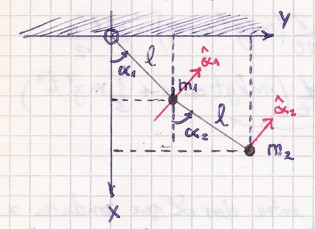
\includegraphics[scale=0.35]{images/fig_mc_clasica_pendulo_doble.jpg}

En principio este problema tiene cuatro coordenadas $x_1,x_2,y_1,y_2$ pero las barras determinan dos ecuaciones de 
vínculo
\[
	x_1^2 + y_1^2 = \ell  \qquad \qquad (x_2-x_1)^2 + (y_2-y_1)^2 = \ell^2
\]
de modo que es un sistema con dos grados de libertad.

\notamargen{Este ejemplo es interesante porque considera unos versores movibles. Habría que continuarlo y ver qué se 
hizo en la carpeta.} 

Para escribir el lagrangiano notemos que 
\[
	T = T_1 + T_2 = \frac 1 2 m_1 ( \dot{x}_1^2 + \dot{y}_1^2 ) + \frac 1 2 m_2 ( \dot{x}_2^2 + \dot{y}_2^2 ) 
\]
\[
	V = -m_1 g x_1 - m_2 g x_2
\]

Y en términos de los ángulos $\alpha_1$, $\alpha_2$ se tiene 
\[
	x_1 = \ell \cos \alpha_1 \qquad y_1 = \ell \sin \alpha_1 
\]
\[
	x_2 = \ell \cos \alpha_2 + \ell \cos \alpha_1 \qquad y_2 = \ell \sin \alpha_1 + \ell \sin \alpha_2
\]
pero antes de hacer toda el álgebra, notemos que $( \dot{x}_1^2 + \dot{y}_1^2 ) = |\vb{v}_1| $ está siempre en la 
dirección del vector $\hat{\alpha}_1$ y no puede tener componente perpendicular. Considerando solamente esa componente, 
sería
\[
	\vb{v}_1 = \ell \: \dot{\alpha}_1 \hat{\alpha}_1 \qquad \text{ con } \qquad v_1^2 = \ell^2 \: \dot{\alpha}_1^2
\]
y correspondientemente
\[
	\vb{v}_2 = \ell \: \dot{\alpha}_1 \hat{\alpha}_1 + \ell \: \dot{\alpha}_2 \hat{\alpha}_2
\]
\[
	v_2^2 = \ell^2 \: \dot{\alpha}_1^2 + \ell^2 \: \dot{\alpha}_2^2 + 2 \dot{\alpha}_1 \dot{\alpha}_2 \ell^2
	\cos ( \alpha_2 - \alpha_1 ).
\]
\end{ejemplo}


% =================================================================================================
\section{Momentos conjugados y coordenadas cíclicas}\index{Momentos conjugados} \index{Coordenadas cíclicas}
% =================================================================================================

Dado un lagrangiano $\Lag = \Lag( q_i,\dot{q}_i, t )$ se define el momento canónicamente conjugado a $q_j$
como 
\be
	p_j \equiv \dpar{\Lag}{\dot{q}_j},
	\label{mom_canon_conj}
\ee
y entonces 
\[
	\dot{p}_j = \frac{d}{dt}\left( \dpar{\Lag}{\dot{q}_j} \right) \equiv Q_j,
\]
que es la fuerza generalizada en el grado de libertad $j$.

Sea ahora un lagrangiano que no depende explícitamente de la coordenada $k$, es decir 
\[
	\Lag = \Lag( q_1,...,q_{k-1},q_{k+1},...,q_n,\dot{q}_1,...\dot{q}_n, t ),
\]
entonces será
\[
	\dpar{\Lag}{q_k}= 0 
\]
y como consecuencia las ecuaciones de Euler-Lagrange en la coordenada $k$-ésima resultan 
\[
	\dtot{}{t}\left( \dpar{\Lag}{\dot{q}_k} \right) = \dot{ p }_k = Q_k = 0 
% 	\quad \rightarrow \;\dot{p}_k = 0 \quad \rightarrow \; p_k = cte.
\]
de manera que no existe fuerza generalizada en el grado de libertad $k$ y como es $\dot{p}_k = 0$, se conserva 
el momento $p_k$ canónicamente conjugado a $q_k$.
En estos casos se dice que la coordenada $q_k$ que no aparece en el lagrangiano, es una coordenada
cíclica.

\begin{ejemplo}{\bf Potencial central en un plano}

Sea un potencial central $ V(r) $ en el plano. El lagrangiano de una partícula de masa $m$ sometida al mismo,
y en las convenientes coordenadas polares $(r,\vp)$ es
\[
	\Lag = \frac{1}{2} m ( \:\dot{r}^2 + r^2 \dot{\vp}^2 ) - V(r).
\]
Luego, las ecuaciones de Euler-Lagrange serán, en $r$,
\[
	\dtot{}{t}\left( \dpar{\Lag}{\dot{r}}\right) - \dpar{\Lag}{r} =
	m\ddot{r} - m\dot{\vp}^2r + \dtot{V}{r} = 0
\]
y en $\vp$
\[
	\dtot{}{t}\left( \dpar{\Lag}{\dot{\vp}}\right) = mr^2\ddot{\vp} = 0.
\]
En esta última debemos notar que $\partial \Lag / \partial \vp = 0 $ y esto significa que $\vp$ es cíclica.
Entonces se conserva el momento canónicamente conjugado a $\vp$ puesto que verifica 
\[
	\dot{p}_\vp = mr^2\ddot{\vp} = 0
\]
lo cual lleva a que $ m r^2\dot{\vp} $ es una constante para este sistema. La moraleja es que la existencia de una 
coordenada cíclica permite ahorrarnos una integración.
Esto, por supuesto, para este problema no es otra cosa que la conservación del momento angular [?].

\end{ejemplo}

% =================================================================================================
\section{Momentos canónicamente conjugados y traslaciones rígidas}
% =================================================================================================

Consideremos un sistema de partículas que sufre una traslación rígida infinitesimal.
Esta traslación se lleva a cabo a través de un desplazamiento en la coordenada $ q $ y de magnitud 
$\delta q$ en la dirección dada por el versor $ \hat{n} $.
% Esta coordenada justamente tiene esa propiedad: una variación de ella representa una 
% traslación rígida.
% ESTE COMENTARIO, que estaba en la carpeta, ahora queda un poco desplazado por la sentencia más
% correcta con respecto a la dirección \hat{n}. Supongo que lo importante es la dirección que en
% el caso de cartesianas la da la misma q pero que en el caso de versores que varían su dirección
% curvilíneos, debe especificarse.

En efecto, para el sistema de $ N $ partículas, la traslación rígida implica
\[
	q \longrightarrow q + \delta q \qquad 
	\vb{x}_i \longrightarrow \vb{x}_i + \delta q \; \hat{n}
\]
La Figura \ref{traslacion_rigida} representa la situación.

Luego, suponiendo una energía cinética de tipo $T_2$, el momento canónicamente conjugado $ p $ (en 
la coordenada $q$ --cuyo subíndice omitimos--) es
\notamargen{[¿se sabe esto a esta altura?]}
\[
	p = \dpar{T}{\dot{q}} = \frac{1}{2} \sum_i^N m_i \left( \dpar{\vb{v}_i^2}{\dot{q}}\right) =
	\sum_i^N m_i \vb{v}_i \cdot \dpar{\vb{v}_i}{\dot{q}} 
\]
\notamargen{Hablar de vectores al cuadrado.\\}
\notamargen{\\ Nota de cómo se manipula: uso $dv^2_i = 2 v_i dv_i$ y}

La {\it forma} de la traslación rígida implica que 
\[
	\dpar{\vb{v}_i}{\dot{q}} = \dpar{\vb{x}_i}{q} = 
	\lim_{\delta q \to 0} \frac{\vb{x}_i + \delta q \:\hat{n} -\vb{x}_i}{\delta q} = \hat{n}.
\]
\notamargen{Recodemos que $ \vb{v}_i = \dot{q}_j\dpar{\vb{x}_i}{q_j} - \dpar{\vb{x}_i}{t} $ }
de modo que 
\[
	p = \sum_i^N m_i \vb{v}_i \cdot \hat{n} = \left( \sum_i^N m_i \vb{v}_i \right) \cdot \hat{n} 
	= \vb{P} \cdot \hat{n} = P_{\hat{n}}
\]

\begin{figure}[htb]
	\begin{center}
	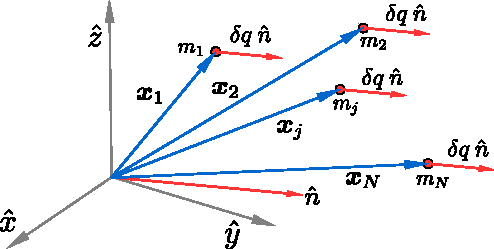
\includegraphics[width=0.6\textwidth]{images/fig_mc_tras_rig.pdf}	 
	\end{center}
	\caption{}
	\label{traslacion_rigida}
\end{figure} 

Hemos arribado al resultado de que el momento canónicamente conjugado correspondiente a la coordenada
generalizada asociada a la traslación rígida es la proyección del momento total en la dirección de ésta.

Para el ejemplo trivial de la partícula libre, $T = 1/2 \; m (\dot{x}^2+ \dot{y}^2+\dot{z}^2)$, se
tiene $ p_x = m v_x $ si la traslación es en la dirección $ \hat{x} $.
\notamargen{Este ejemplo suma algo?}

Para las fuerzas generalizadas, equivalentemente se tiene 
\[
	Q = \sum_i^N \vb{F}^a_i \cdot \dpar{\vb{x}_i}{q} =
	\left( \sum_i^N \vb{F}^a_i \right) \cdot \hat{n} = \vb{F}\cdot \hat{n},
\]
la fuerza generalizada es la proyección de las fuerzas aplicadas en la dirección dada por $ \hat{n} $.

\notamargen{Revisar porque esto no estaba tan claro. Supongo que la idea es ver que aún con presencia
de $T_1$ esto sigue valiendo}
La ecuación para la fuerza generalizada $Q_j$ era
\[
	Q_j = \frac{d}{dt}\left( \dpar{T}{\dot{q}_j} \right) - \dpar{T}{q_j}.
\]
Aún en el caso de que $T$ dependa de $q_j$ la traslación rígida implica que 
$ \partial{T}/\partial{q_j} = 0 $ 
porque es sumar un vector constante a la posición, luego $ d\vb{x}_i/dt = d(\vb{x}_i + \vb{a}) /dt$
para todo \vb{a} constante. Entonces, para la coordenada q asociada a la traslación en $\hat{n}$
se tiene 
% \[
% 	Q_j = \frac{d}{dt}\left( \dpar{T}{\dot{q}_j} \right)
% \]
% y en el caso de la traslación con dirección $\hat{n}$,
\[
	Q = \frac{d}{dt}\left( \dpar{T}{\dot{q}} \right) = \dtot{P_{\hat{n}}}{t},
\]
de tal manera que si en $\hat{n}$ no hay fuerza $Q$ tendremos $ d P_{\hat{n}}/dt = 0 $, es decir 
$ P_{\hat{n}} $ conservado.

\notamargen{Acá la cosa es que la traslación es una cosa que sufre el sistema pero no es dinámica.
Es una construcción nuestra, como un cambio de sistema de referencia.}

% pero el segundo término del lado izquierdo $\partial T/\partial q_j = 0$ puesto que la $T$ no se ve
% afectada por cambiar trasladando rígidamente el sistema.
% \[
% 	\frac{d}{dt}(\vb{p}\cdot \hat{n}) = \vb{F}\cdot \hat{n},
% \]
% y esto significa que el $p_j$ se conserva si no hay fuerza en $\hat{j}$.

% =================================================================================================
\section{Momentos canónicamente conjugados y rotaciones rígidas}
% =================================================================================================

Ahora consideraremos un sistema de partículas que sufre una rotación rígida infinitesimal.
Esta se materializa a través de un desplazamiento angular en la coordenada $ q $ de magnitud $\delta q$.
La dirección y sentido, para cada posición $ \vb{x}_i $ vienen dadas por el producto vectorial 
$ \hat{n} \times \vb{x}_i$.

\notamargen{Esta coordenada $q$ es especial en el sentido en que representa una rotación.}
Para un sistema de $ N $ partículas, la rotación rígida implica
\[
	q \longrightarrow q + \delta q |\vb{x}| \sin \alpha_i \qquad
	\vb{x}_i \longrightarrow \vb{x}_i + \delta q \; \hat{n} \times \vb{x}_i
\]
La Figura \ref{rotacion_rigida} representa la situación, donde por razones de claridad se muestran
solamente dos partículas.

\begin{figure}[htb]
	\begin{center}
	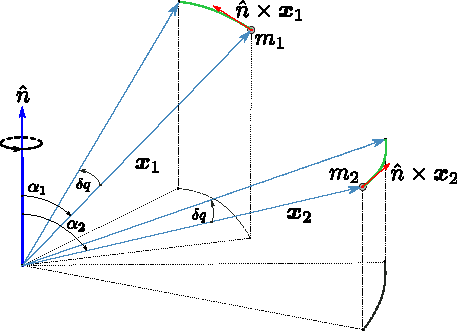
\includegraphics[width=0.6\textwidth]{images/fig_mc_rot_rig.pdf}	 
	\end{center}
	\caption{}
	\label{rotacion_rigida}
\end{figure} 
% Ahora es el turno de la rotación rígida. Sea coordenada que representa rotación rígida,
% \[
% 	\vb{r}_i \longrightarrow \vb{r}_i + \delta q (\hat{n} \times \vb{r}_i)
% \]
El momento canónicamente conjugado en la coordenada angular $q$ será
\[
	p = \dpar{T}{\dot{q}} = 
	\sum_i^N m_i \vb{v}_i \cdot \dpar{\vb{v}_i}{\dot{q}} =
	\sum_i^N m_i \vb{v}_i \cdot \hat{n} \times \vb{x}_i = 
	\sum_i^N m_i \vb{v}_i \cdot ( \hat{n} \times \vb{x}_i )
\]
donde hemos utilizado el hecho de que 
\[
	\dpar{\vb{v}_i}{\dot{q}} = \dpar{\vb{x}_i}{q} = 
	\lim_{\delta q \to 0} \frac{ \vb{x}_i +\delta q (\hat{n} \times \vb{x}_i)- 
	\vb{r}_i}{\delta q} = \hat{n} \times \vb{x}_i. 
\]

El sumando se puede reescribir (usando $\vb{A}\cdot(\vb{B}\times\vb{C}) = 
\vb{B}\cdot(\vb{C}\times\vb{A})$) para que aparezca explícitamente la forma buscada,
\[
	p = \sum_i^N m_i \vb{v}_i \cdot ( \hat{n} \times \vb{x}_i ) =
	\sum_i^N \hat{n} \cdot ( \vb{x}_i \times m_i \vb{v}_i  ) =
	\sum_i^N \hat{n} \cdot \vb{l}_i = \hat{n} \cdot \sum_i^N \vb{l}_i =
	\hat{n} \cdot \vb{L}
\]
que significa
\[
	p = \hat{n} \cdot \vb{L} = L_{\hat{n}},
\]
el momento canónicamente conjugado en la dirección $\hat{n}$ es el momento angular total
del sistema proyectado en esa dirección.
% \[
% 	|\delta q(\hat{n} \times \vb{r}_i)| = \delta q r_i \sin (\alpha)
% \]
% El momento canónicamente conjugado en la dirección $\hat{n}$ es el $\vb{L}$ proyectado en esa dirección.
% \[
% 	\frac{d}{dt}(\hat{n}\cdot\vb{L}) = \hat{n}\cdot\vb{\tau}
% \]
% y el $p_j$ se conserva si no hay torque.
La fuerza generalizada será
\[
	Q = \sum_i^N \vb{F}^a_i \cdot \dpar{\vb{x}_i}{q} = 
	\sum_i^N \vb{F}^a_i \cdot ( \hat{n} \times \vb{x}_i ) = 
	\hat{n} \cdot \left( \sum_i^N \vb{x}_i \times  \vb{F}^a_i \right) = 
	\hat{n} \cdot \sum_i^N \vb{\tau}_i = \hat{n} \cdot \vb{\Tau},
\]
i.e. la componente del torque en la dirección $ \hat{n} $.

Asimismo, si la coordenada implica una rotación rígida entonces $ \partial{T}/\partial{q} = 0 $ 
debido a que la energía cinética $ T $ es un escalar y es por ende invariante ante rotaciones
(un vector rotado cambia su dirección pero no su módulo).
Luego
\[
	Q = \frac{d}{dt}\left( \dpar{T}{\dot{q}} \right) = \dtot{L_{\hat{n}}}{t} = \vb{\Tau}_{\hat{n}}.
\]
% \[
% 	\frac{d}{dt}\left( \hat{n}\cdot \vb{L} \right) = \hat{n}\cdot \vb{\tau}
% \]
\notamargen{Tal vez un ejemplo 2D ayude a aclarar un poco este tema.}

Todo este análisis (traslaciones y rotaciones rígidas) vale si el potencial $V$ no depende de la
velocidad; en caso contrario cambia la forma de los momentos canónicos. En efecto, en este caso
es
\[
	p = \dpar{ \Lag }{\dot{q}} = \dpar{(T-V)}{\dot{q}}
\]
Volviendo al ejemplo de la partícula de masa $m$ y carga $q$ en un campo electromagnético se tendrá
\[
	p = m v_{\hat{n}} + \frac{q}{c} \vb{A}\cdot\hat{n},
\]
es decir que aparece un término extra con el potencial vector respecto del caso en que la partícula
está libre.

% =================================================================================================
\section{Energía cinética de un sistema}\index{Energía cinética}
% =================================================================================================

Resulta útil disponer de la energía cinética de un sistema en función de coordenadas generalizadas.
Para un sistema de $N$ partículas, es 
\[
	T = \frac{1}{2} \sum_i^N m_i |\vb{v}_i|^2 
\]
donde las posiciones de cada una de ellas se pueden expresar en términos de $k$ coordenadas generalizadas
\[
	\vb{x}_i = \vb{x}_i(q_1, q_2, ..., q_k, t )
\]
y sus respectivas velocidades serán
\notamargen{La derivada con respecto al tiempo de la posición es la $ d/dt $ no la parcial.}
\[
	\vb{v}_i = \sum_j^{k}  \dpar{\vb{x}_i}{q_j} \: \dot{q}_j + \dpar{\vb{x}_i}{t}.
\]
\notamargen{Este chapter es básicamente un desarrollo formal, habría que bajar con alguna aplicación práctica.}
Luego, utilizando el hecho de que $ |\vb{v}_i|^2 = \vb{v}_i \cdot \vb{v}_i $, se tiene 
\be
	T = \frac{1}{2} \sum_i^N m_i \left( \sum_{j=1}^{k}  \dpar{\vb{x}_i}{q_j}\dot{q}_j + \dpar{\vb{x}_i}{t} \right)
	\cdot \left( \sum_{s=1}^{k} \dpar{\vb{x}_i}{q_s}\dot{q}_s + \dpar{\vb{x}_i}{t} \right) 
\label{mc_T}
\ee
y expandiendo el producto resulta
\[
	T = \frac{1}{2} \sum_i^N m_i \left[ \sum_j^{k}\sum_s^{k} \dpar{\vb{x}_i}{q_j} \cdot \dpar{\vb{x}_i}{q_s}\dot{q}_s\dot{q}_j + 
	2 \dpar{\vb{x}_i}{t} \cdot \sum_j^{k} \dpar{\vb{x}_i}{q_j}\dot{q}_j + \left| \dpar{\vb{x}_i}{t} \right|^2 \right],
\]
la cual se puede separar en tres contribuciones
\[
	T = T_2 + T_1 + T_0
\]
\notamargen{Sacarle espacio al \texttt{cdot}}
con las siguientes formas:
\[
	T_2 = \frac{1}{2} \sum_j^{k} \sum_s^{k} \left( \sum_i^N m_i \dpar{\vb{x}_i}{q_j} \cdot \dpar{\vb{x}_i}{q_s} \right) \dot{q}_j\dot{q}_s
\]
\[
	T_1 =  \sum_j^{k} \left( \sum_i^N m_i \dpar{\vb{x}_i}{t} \cdot \dpar{\vb{x}_i}{q_j} \right) \dot{q}_j
\]
\[
	T_0 = \frac{1}{2} \sum_i^N m_i \left| \dpar{\vb{x}_i}{t} \right|^2,
\]
donde se ha alterado el orden de los signos $\sum$ para enfatizar el hecho de que las cantidades entre paréntesis pueden asociarse
a una matriz y un vector de acuerdo con 
\[
	a_{js}(q_1,...,q_k,t) \equiv \sum_i^N  m_i \dpar{\vb{x}_i}{q_j} \cdot \dpar{\vb{x}_i}{q_s}
\]
\[
	b_j(q_1,...,q_k,t) \equiv \sum_i^N  m_i \dpar{\vb{x}_i}{q_j} \cdot \dpar{\vb{x}_i}{t}
\]

Entonces
\[
	T_2 = \frac{1}{2} \sum_j^{k} \sum_s^{k} \: a_{js} \: \dot{q}_s\dot{q}_j, \qquad 
	T_1 = \sum_j^{k} \: b_j \: \dot{q}_j , \qquad 
	T_0 = \frac{1}{2} \sum_i^N m_i \left| \dpar{\vb{x}_i}{t} \right|^2
\]
son, respectivamente, contribuciones cuadráticas, lineales o de orden cero con respecto a las velocidades generalizadas $\dot{q}$.
% 
% Usando $\vb{r}_i = \vb{r}_i(q_1, ...,q_n,t)$ desarrollamos un desplazamiento real como
% \[
% 	d\vb{r}_i = \sum_{j=1}^{3N-k} \left( \dpar{\vb{r}_i}{q_j} \right) dq_j + \dpar{\vb{r}_i}{t} dt
% \]
% y podemos incorporar esta información en \eqref{mc_T} para obtener
% \[
% 	T = 
% 	\frac{1}{2} \sum_i^N m_i \left( \sum_j^{3n-k}\sum_s^{3n-k}  
% 	\dpar{\vb{r}_i}{q_j}\dpar{\vb{r}_i}{q_s}\dot{q}_s\dot{q}_j + 
% 	\left( \dpar{\vb{r}_i}{t} \right) \right)^2 +
% 	2 \left( \sum_j^{3n-k} \dpar{\vb{r}_i}{q_j}\dot{q}_j\dpar{\vb{r}_i}{t} \right) 
% \]
% \[
% 	T = 
% 	\frac{1}{2} \sum_i^N m_i \left( \sum_j^{3n-k}\sum_s^{3n-k}  
% 	\dpar{\vb{r}_i}{q_j}\dpar{\vb{r}_i}{q_s}\dot{q}_s\dot{q}_j  \right) + 
% 	\frac{1}{2} \sum_i^N m_i \left( \dpar{\vb{r}_i}{t} \right)^2 +
% 	\sum_i^N m_i \left( \sum_j^{3n-k} \dpar{\vb{r}_i}{q_j}\dot{q}_j\dpar{\vb{r}_i}{t} \right) 
% \]

Para una particula libre será
\[
	T = T_2
\]
es decir que solamente es cuadrática en las velocidades. Para una partícula sometida a vínculos en general, en términos
de las coordenadas generalizadas, se tendrán las tres clases de cinética.

En coordenadas esféricas la energía de una partícula libre es 
\[
	T_2 =  \frac{1}{2} m \left( \dot{r}^2 + r^2 \dot{\theta}^2 + r^2 \sin \theta \dot{\vp}^2 \right).
\]
Si las coordenadas generalizadas son las coordenadas $ r, \theta, \vp $ se identifica 
\[
	T_2 =  \frac{1}{2} m \left( a_r(r, \theta, \vp ) \dot{r}^2 + a_\theta(r, \theta, \vp ) \dot{\theta}^2 + 
	a_\phi(r, \theta, \vp ) \dot{\vp}^2 \right).
\]

% =================================================================================================
\section{Energía cinética de un sistema de partículas}
% =================================================================================================

La energía de un sistema de partículas es 
\begin{multline*}
	T = \frac{1}{2} \sum_i^N m_i \vb{v}_i^2 = 
	\frac{1}{2} \sum_i^N m_i \left( \dot{\vb{R}} + \dot{\vb{r}}_i' \right)^2 = \\
	\frac{1}{2} \sum_i^N m_i \vb{V}_{cm}^2  +
	\frac{1}{2} \sum_i^N m_i \vb{V}_i'^2 +
	\frac{1}{2} \sum_i^N 2 m_i \vb{V}_{cm} \cdot  \vb{r}_{i}' 
\end{multline*}
y veremos ahora que el último término es nulo ya que son vectores perpendiculares.
Para ello notemos que 
\[
	M \vb{R}_{cm} = \sum_i^N m_i \vb{r}_i = \sum_i^N m_i ( \vb{R}_i + \vb{r}_i' )
\]
\[
	0 = \sum_i^N m_i \vb{r}_i'
\]
y también 
\[
	0 = \sum_i^N m_i \vb{v}_i'
\]
de modo que 
\[
	0 = \sum_i^N m_i \vb{V}_{cm} \cdot \vb{r}_i'.
\]
\notamargen{Esto hay que revisarlo, derivo ambos miembros? Vincular con la figura.}
Finalmente 
\[
	T^{tot} = T^{cm} + T_{cm}^{tot}
\]

\begin{figure}
	\begin{center}
	\includegraphics[width=0.3\textwidth]{images/fig_sist_part.pdf}	 
	\end{center}
	\caption{Sistema de partículas}
\end{figure} 

% =================================================================================================
\section{Trabajo en un sistema de partículas}
% =================================================================================================

Empezamos desde
\[
	W = W^{ext} + W^{int}
\]
donde el trabajo externo puede escribirse
\notamargen{Quiero un $\ell$ en bold, no me gusta el ${\bf s}$.}
\be
	W^{ext} = \sum_i^N \int_1^2 \vb{F}_i^e \cdot d\vb{s}
\label{mc_work_ext}
\ee

La no dependencia del camino para la integral que da \eqref{mc_work_ext} requiere que 
\[
	\vb{F}_i^e = \vb{F}_i^e( \vb{r}_i ) \qquad \nabla_{r_i} \times \vb{F}_i^e = 0
\]
y entonces puedo inducir la existencia de una función potencial para las fuerzas externas,
\notamargen{barra resizeable ya.}
\[
	W^{ext} = - \sum_i^N  \left. \Delta V_i \right]_1^2 
\]

Por otro lado,
\[
	W^{int}_c = \int_1^2 \sum_{\substack{j\\j\neq i}}^N  \vb{F}_{ij}^e \cdot d\vb{s}_i  
\]
\[
	\sum_i^N W_i^{int} =  W^{int} = \sum_{\substack{j \\ i\neq j}}^N  
	\int_1^2 \sum_{\substack{j \\ j\neq i}}^N  \vb{F}_{ij}^e \cdot d\vb{s}_i  
\]

% =================================================================================================
\section{Lagrangiano cíclico en el tiempo}
% =================================================================================================

Empezando desde la derivada total con respecto al tiempo del lagrangiano,
\be
	\frac{d}{dt}\left( \Lag( q, \dot{q}, t)\right) =
	\dpar{\Lag}{q} \dot{q} + \dpar{\Lag}{\dot{q}} \ddot{q} + \dpar{\Lag}{t}
	\label{derivada_lag_ciclico}
\ee
y usando la derivada total del término 
\[
	\frac{d}{dt}\left( \dpar{\Lag}{\dot{q}}\dot{q}\right) =
	\frac{d}{dt}\left( \dpar{\Lag}{\dot{q}} \right) \dot{q} + \dpar{\Lag}{\dot{q}} \ddot{q},
\]
se puede expresar \eqref{derivada_lag_ciclico} sin derivadas segundas explícitas $\ddot{q}$ de suerte que 
\[
	\frac{d}{dt}\left( \Lag( q, \dot{q}, t)\right) = \dpar{\Lag}{q} \dot{q} + \frac{d}{dt}\left( 
	\dpar{\Lag}{\dot{q}}\dot{q}\right) - \frac{d}{dt}\left( \dpar{\Lag}{\dot{q}} \right) \dot{q} + \dpar{\Lag}{t}
\]
la cual, acomodando un poco los términos, resulta en
\[
	\frac{d}{dt}\left( \Lag( q, \dot{q}, t)\right) = 
	\left[ \dpar{\Lag}{q}  - \frac{d}{dt}\left( \dpar{\Lag}{\dot{q}} \right) \right] \dot{q} + 
	\frac{d}{dt}\left( \dpar{\Lag}{\dot{q}}\dot{q}\right)  + \dpar{\Lag}{t}.
\]

Como el corchete son las ecuaciones de Euler-Lagrange y además $\partial\Lag/\partial \dot{q} \equiv p$ se tiene
\[
	\frac{d}{dt}\left( \Lag( q, \dot{q}, t)\right) = \frac{d}{dt}\left( p \: \dot{q} \right) + \dpar{\Lag}{t},
\]
o bien,
\[
	\frac{d}{dt}\left( p \: \dot{q} - \Lag \right) = -\dpar{\Lag}{t}.
\]
Definiendo al operador hamiltoniano $\Ham$ como 
\be
	\Ham \equiv p\:\dot{q} - \Lag 
	\label{hamiltoniano}
\ee
resulta que 
\be
	\dtot{\Ham}{t} = - \dpar{\Lag}{t}
	\label{derivada_temporal_ham}
\ee

El hamiltoniano es un operador tal que su variación temporal total depende de la variación temporal explícita del 
lagrangiano.
Entonces, si el lagrangiano no depende explícitamente del tiempo se tiene que $ \Ham = \Ham_0 $, el hamiltoniano
se conserva.\footnote{Notemos en la ecuación \eqref{derivada_temporal_ham} que la derivada $ \partial \Lag / \partial t$ 
refiere a la aparición explícita de $ t $; de este modo el hecho de que sea $ \partial \Lag / \partial t = 0 $ significa
que el $\Ham$ se conserva pero no que $\Lag$ se conserva. Esto último requeriría $ d \Lag / dt = 0 $.}

\notamargen{No sé en qué momento se ha definido el hamiltoniano, $H=T+V$, deberíamos referirlo y tenerlo en cuenta.}

Por otra parte, si se cumple que :
\begin{itemize}
 \item Los vínculos no dependen del tiempo
 \item El potencial no depende de las velocidades generalizadas,
\end{itemize}
entonces el hamiltoniano es la energía, es decir 
\be
	\Ham = E = T + V.
	\label{hamiltoniano_energia}
\ee

La condición de que los vínculos no dependan del tiempo tiene como consecuencia que la energía cinética sea una 
función cuadrática en las velocidades generalizadas. Entonces la condición \eqref{hamiltoniano_energia} se puede
expresar en términos de las energías cinéticas y potenciales como 
\[
	T = T_2   \qquad   \qquad   V \neq V(\dot{q})
\]

Asimismo, la condición de energía constante $ E = E_0 $ se cumplirá si el trabajo de las fuerzas no conservativas
es nulo, $ W^{\text{nc}} = 0 $.
\notamargen{Esto se debiera haber visto antes en algún momento, y convendría recordarlo aquí.}

\begin{ejemplo}{\bf Bola rotante engarzada en alambre}

Una barra gira sobre un mesa sin rozamiento en torno a un punto fijo $O$ con velocidad angular constante $ \omega $.
Esta barra tiene enhebrada una bola de masa $m$ que puede deslizarse libremente a lo largo de la misma, como se ilustra 
esquemáticamente en la figura \ref{fig_barra_giratoria}.

\begin{figure}[bth]
	\begin{center}
	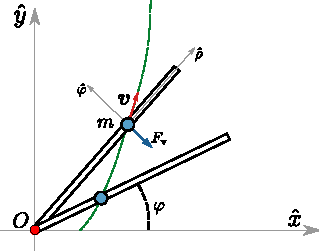
\includegraphics[width=0.4\textwidth]{images/fig_barra_giratoria.pdf}
	\end{center}
	\caption{Problema de la barra que gira con una masa $m$ enhebrada.}
	\label{fig_barra_giratoria}
\end{figure} 

Claramente la bola seguirá, con respecto a un sistema de coordenadas polar $(\rho,\vp)$ con origen en el punto $O$,
una trayectoria como la esquematizada por la curva verde. 
% Las coordenadas generalizadas son $\rho,\vp$

En este problema no hay potencial y el lagrangiano, que es $T$, será 
\[
	\Lag = \frac{1}{2} ( \dot{\rho}^2 + \rho^2 \omega^2 )
\]

El hamiltoniano es 
\be
	\Ham = \frac{1}{2} ( \dot{\rho}^2 - \rho^2 \omega^2 ).
	\label{ham_ejemplo_bola}
\ee
Luego, como el lagrangiano no depende explícitamente del tiempo entonces el hamiltoniano dado por la \eqref{ham_ejemplo_bola}
se conserva. No obstante, el hamiltoniano no es la energía puesto que la energía cinética $ T $ tiene la forma  $ T = T_2 + T_0 $,
que proviene del hecho de que la fuerza de vínculo (que tendrá dirección angular en este caso) dependerá del tiempo.
La energía no se conserva, claramente hay trabajo de la fuerza de vínculo, que es una fuerza no conservativa. 

La conservación del hamiltoniano dependerá de las coordenadas generalizadas elegidas. Podría pensarse que el $\Ham$ es la energía
vista en un sistema no inercial [?].
La energía siempre es la medida en un sistema inercial. Además, cuando se conserve lo será desde cualquier sistema de coordenadas
inercial elegido.
 
\end{ejemplo}


% =================================================================================================
\section{Energía cinética y el hamiltoniano}
% =================================================================================================

Dado que la energía cinética tiene la forma general
\[
	T = \underbrace{\frac{1}{2} \sum_i^N m_i \left( \dpar{\vb{r}_i}{t} \right)^2}_{T_0}  +
	\underbrace{\sum_j^{3n-k} b_j(q_1,...,q_{3N-k},t)\dot{q}_j  }_{T_1} +
	\underbrace{\frac{1}{2} \sum_j^{3n-k}\sum_s^{3n-k}  a_{js}(q_1,...,q_{3N-k},t)\dot{q}_s\dot{q}_j }_{T_2}
\]
entonces se sigue que 
\be
	E = T_0 + T_1 + T_2 + V
\label{mc_E}
\ee
y como 
\[
	p_i = \dpar{\Lag}{\dot{q}_i} = T_1 + 2T_2 
\]
es 
\[
	\Ham = \sum_i^N p_i\dot{q}_i - (T_0 + T_1 + T_2 - V) = 2T_2 + T_1 - T_0 - T_1 - T_2 + V = T_2 - T_0 + V
\]
pero como E es \eqref{mc_E} se tendrá 
\[
	E = H \iff 2T_0 + T1 = 0
\]
y un solución de este sistema es, por supuesto, $T_0 = T_1 = 0$

% =================================================================================================
\section{Principio de acción mínima}
% =================================================================================================

El estado de un sistema mecánico de $ N $ grados de libertad en un dado instante de tiempo $ t $ puede asociarse a 
un vector de componentes $ \{ q_i \} $ viviendo en un espacio $N$-dimensional de coordenadas generalizadas. 
La evolución entre dos puntos en ese espacio, de $ \{ q_i(t_a) \} $  a $ \{ q_i(t_b) \} $ por ejemplo, se realiza por
un trayecto continuo entre esos dos puntos, que es la trayectoria del sistema.

\begin{figure}[bth]
	\begin{center}
	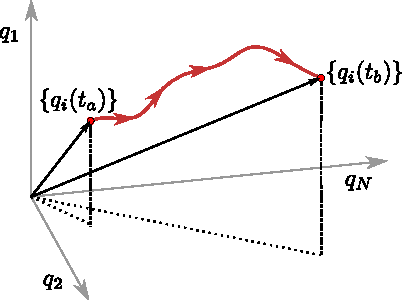
\includegraphics[width=0.5\textwidth]{images/fig_hamilton.pdf}	 
	\end{center}
	\caption{Trayectoria de un sistema mecánico $\{ q_i \}$ entre dos puntos del espacio $N$-dimensional de
	coordenadas generalizadas.}
	\label{principio_hamilton}
\end{figure}

En principio cualquier trayecto entre dos puntos es posible porque eso depende de la física a la cual está sometido
el sistema, no obstante existe un principio que permite saber cuál es la trayectoria que seguirá.

Considerando el lagrangiano $ \Lag = T - V $ y la siguiente integral (la acción $S$) entre los puntos $ \{ q_i(t_a) \} $
y $ \{ q_i(t_b) \} $,
\[
	S = \int_{t_a}^{t_b} \Lag( q_1(t, q_2(t), ..., \dot{q}_1(t),\dot{q}_2(t), ...,t )) \: dt
\]
se tiene que la trayectoria real entre estos dos puntos es tal que la integral $S$ toma su valor mínimo.

Dicho de otra manera, esto significa que $ S $ como funcional dependiendo de $ \{ q_i \}, \{ \dot{q}_i \} $
deberá tener un valor mínimo (o ser estacionaria) al especializarse en la trayectoria real.
Esto es análogo a lo que sucede en cálculo; en el mínimo de una función (de una o varias variables) la derivada 
se anula. El concepto equivalente en funcionales como $ S $ es el de variación nula.

La idea es construir una {\it variación} arbitraria respecto de la trayectoria real $ \{ q_i \} $ y forzar a que esa 
variación se anule para obtener un condición sobre las $ \{ q_i \} $ (para funciones esa condición era que el gradiente
se anule).

Si me sitúo en la trayectoria verdadera, es decir el conjunto $ \{ q_i(t) \}$, una variación arbitraria de la misma
tendrá la forma
\be
	q_i(t) \rightarrow q_i(t) + \delta q_i(t) \qquad i=1,2, ...
	\label{variacion}
\ee
donde cada coordenada $ q $ variará de acuerdo con su correspondiente desplazamiento $\delta q $.
La variación se hace en un intervalo de tiempo arbitrario $ [t_a,t_b] $ y con extremos fijos, 
\be
	\delta q(t_a) = 0 \qquad \qquad \delta q(t_b) = 0,
	\label{extremos_fijos}
\ee
lo que significa que los puntos de partida y llegada en el espacio de fases son los mismos.
\notamargen{Habría que justificar cuál es el significado de esto y porqué es así.}

Asimismo se pedirá que todas las trayectorias empleen el mismo tiempo de manera que la variación se hará en algún
tiempo fijo intermedio $ t_a < t < t_b $. O sea que $\delta t = 0$.

\notamargen{Cuán sketchi es todo esto!! Mucho para aclarar. Tal vez se justifique un minicurso de variacional como 
apéndice.}

Una representación unidimensional (una única $q$) puede verse en la Figura \ref{principio_accion_minima}.
La trayectoria real sería la curva $ q(t) $ en color rojo, mientras que la curva verde sería una trayectoria variada
a través de $ \delta q $. Los extremos fijos \eqref{extremos_fijos} implican que la variación es nula allí, y entonces
las curvas comienzan y terminan en el mismo punto.

\begin{figure}
	\begin{center}
	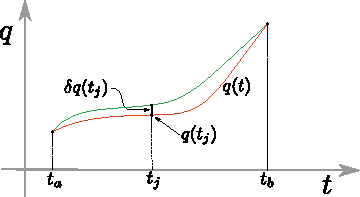
\includegraphics[width=0.7\textwidth]{images/fig_accion.pdf}	 
	\end{center}
	\caption{El principio de acción mínima}
	\label{principio_accion_minima}
\end{figure}

El hecho de considerar una variación a tiempo fijo $t_j$ implica que nos situaremos arbitrariamente en ese instante
y variaremos las trayectorias $ \{ q_i \} $ congeladas en ese instante arbitrario. Por supuesto, el resultado debería
valer para cualquier instante intermedio considerado.

La idea es determinar las condiciones que se necesitan para 
\[
	\frac{\delta S}{\delta q_i} = 0.
\]

Para ello comenzamos tomando una variación de $S$ que pasa dentro de la integral como 
\[
	\delta S = \int \left[ \Lag(q_i + \delta q_i, \dot{q}_i + \delta \dot{q}_i , t )
	- \Lag(q_i , \dot{q}_i , t ) \right] dt
\]
y donde vemos explícitamente que es a tiempo fijo.

La variación de la integral puede escribirse 
\[
	\delta S =  \int_{t_a}^{t_b} \sum_i^N \left( \dpar{\Lag}{\dot{q}_i} \delta \dot{q}_i +
	\dpar{\Lag}{q_i} \delta q_i  \right) dt,
\]
y como será útil tener todo en función de las variaciones $\delta q_i$, es conveniente expresar las variaciones $ 
\delta \dot{q}_i $ en términos de una derivada total a través de  
\[
	\frac{d}{dt}\left( \dpar{\Lag}{\dot{q}_i} \delta q_i \right) =
	\frac{d}{dt}\left( \dpar{\Lag}{\dot{q}_i} \right) \delta q_i + \dpar{\Lag}{\dot{q}_i}\delta \dot{q}_i,
\]
resultando en 
\[
	\delta S =  \int_{t_a}^{t_b} \sum_i^N \left[ \frac{d}{dt}\left( \dpar{\Lag}{\dot{q}_i} \delta q_i \right) -
	\frac{d}{dt}\left( \dpar{\Lag}{\dot{q}_i} \right) \delta q_i + \dpar{\Lag}{q_i} \delta q_i  \right] dt,
\]
que se puede separar en dos términos
\[
	\delta S =  \int_{t_a}^{t_b} \sum_i^N \left[ \frac{d}{dt}\left( \dpar{\Lag}{\dot{q}_i} \delta q_i \right) 
	\right] dt + \int_{t_a}^{t_b} \sum_i^N \left[ \dpar{\Lag}{q_i} - \frac{d}{dt}\left( \dpar{\Lag}{\dot{q}_i} 
	\right) \right]  \delta q_i \; dt,
\]

Pero el primer término es una derivada total y por el teorema fundamental del cálculo,
\be
	\int_{t_a}^{t_b} \sum_i^N \left[ \frac{d}{dt}\left( \dpar{\Lag}{\dot{q}_i} \delta q_i \right) \right] dt =
	\sum_i^N \left. \dpar{\Lag}{\dot{q}_i} \delta q_i \: \right|_{t_a}^{t_b}
\label{mc_borde_term}
\ee
y es nulo porque $\delta q_i=0$ en los extremos para toda coordenada $i$ (las variaciones son nulas en los extremos). 
Decimos que este es un término de superficie. Entonces la condición 
\[
	\delta S =  \sum_i^N  \int_{t_a}^{t_b}
	\left[ \dpar{\Lag}{q_i} - \frac{d}{dt}\left( \dpar{\Lag}{\dot{q}_i} \right)  \right]  \delta q_i  dt = 0
\]
se verificará por el cumplimiento de las ecuaciones de Euler-Lagrange\footnote{Como las variaciones $\delta q_i$ son 
arbitrarias e independientes la anulación de la ecuación $ \delta S $ requiere la anulación de cada uno de los 
$i=1,2,...N $ corchetes en los integrandos.}
\[
	\sum_i^N  \left[ \frac{d}{dt}\left( \dpar{\Lag}{\dot{q}_i} \right) - \dpar{\Lag}{q_i} \right] = 0.
\]

Se puede ver que 
\[
	\delta S = 0 \quad \iff \quad \sum_i^N  \left[ \frac{d}{dt}\left( \dpar{\Lag}{\dot{q}_i} \right) -
	\dpar{\Lag}{q_i} \right] = 0.
\]


Luego, si se hace $\Lag' = \Lag + df/dt$ (ambos lagrangianos difieren en una derivada total con 
respecto al tiempo) la trayectoria que minimiza $\Lag'$ es la que misma que minimiza
$\Lag$ por la condición dada por \eqref{mc_borde_term}. 

La moraleja es que si los lagrangianos difieren en una derivada total del tiempo obtenemos la misma
física.

\begin{ejemplo}{\bf Problema círculos}

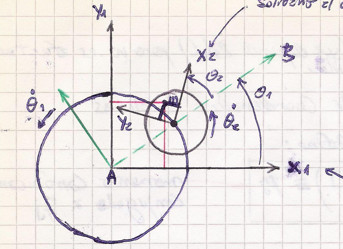
\includegraphics[scale=0.3]{images/fig_mc_dos_circulos_rotantes.jpg} 
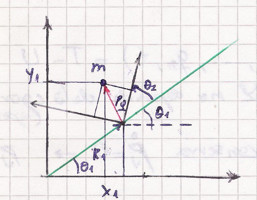
\includegraphics[scale=0.3]{images/fig_mc_dos_circulos_subsistema.jpg} 
 
El disco pequeño está solidario al disco [?]. La línea AB está pintada sobre los discos para poder medir los ángulos.
El eje $x_1$ está solidario al piso (inercial).

La segunda figura ilustra el movimiento de la masa en el sistema fijo.,
\[
	x_1 = R_1 \cos \theta_1 + \rho \cos ( \theta_1 + \theta_2 + \vp )
\]
\[
	y_1 = R_1 \sin \theta_1 + \rho \sin ( \theta_1 + \theta_2 + \vp )
\]
Luego, hay que calcular 
\[
	\frac 1 2 m |\vb{v}|^2
\]
con 
\[
	\dot{x}_1 = -R_1 \sin \theta_1 \dot{\theta}_1 + \dot{\rho} \cos ( \theta_1 + \theta_2 + \vp ) -
	\rho ( \dot{\theta}_1 + \dot{\theta}_2 + \dot{\vp} ) \sin( \theta_1 + \theta_2 + \vp )
\]
\[
	\dot{y}_1 = R_1 \cos \theta_1 \dot{\theta}_1 + \dot{\rho} \sin ( \theta_1 + \theta_2 + \vp ) +
	\rho ( \dot{\theta}_1 + \dot{\theta}_2 + \dot{\vp} ) \cos( \theta_1 + \theta_2 + \vp )	
\]

Habría que elevar esto al cuadrado, lo cual a mano es un trabajo un poco cumbersome.
\[
	T = \frac 1 2 m ( R_1^2 \dot{\theta}_1^2 + \rho^2( \dot{\theta}_1 + \dot{\theta}_2  + \dot{\vp} ) + \dot{\rho}^2 + 
	2R_1\dot{\theta}_1\left[ \dot{\rho}\sin(\theta_2+\vp) + \rho( \dot{\theta}_1 + \dot{\theta}_2 + \dot{\vp} )\cos(\theta_2+\vp) \right])
\]
y como no hay potencial, entonces $\Lag = T $. Trabajando con las ecuaciones de Lagrange se llega a
\[
	\ddot{\rho} - \rho ( \omega_1 + \omega_2 + \dot{\vp} )^2 - R_1 \omega_1^2 \cos (\omega_2 t + \vp ) = 0
\]
\[
	\ddot{\vp} + \frac{\dot{\rho}}{\rho}\left[ 2(\omega_1 + \omega_2 )\right] + 
	\frac{R_1\omega_1( \omega_1 + \omega_2 )}{\rho} \sin (\omega_2 t + \vp ) = 0
\]

Este sistema tiene dos grados de libertad $(\rho,\vp)$ y el lagrangiano es $\Lag(\vp,\rho,\dot{\vp},\dot{\rho},t)$. En realidad
$\dot{\theta}_j = \dot{\theta}_j(\rho\vp)$ para $j=1,2$ y entonces $\theta_j$ no son coordenadas generalizadas.

Este problema se puede simplificar si se asume que $ \dot{\theta}_1, \dot{\theta}_2 $ son constantes [Esto viene antes o viene después].
\end{ejemplo}


\begin{ejemplo}{\bf Problema 17}
 
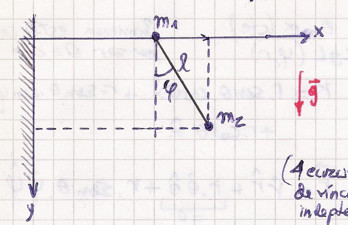
\includegraphics[scale=0.3]{images/fig_mc_pendulo_deslizante.jpg} 

Un problema de dos masas con, en principio, seis grados de libertad. Dado que el movimiento se asume que ocurre en un plano, el $z$
por ejemplo, eso implica dos vínculos $z_1 = z_2 = 0$ a los cuales debemos sumarle la fijación de $m_1$ en la altura $y_1 = 0$ y el vínculo 
de la barra
\[
	y_2^2 + (x_2 -x_1)^2 = \ell^2
\]
luego es un problema de dos grados de libertad, que pueden ser elegidos como $(x,\vp)$. Esto último puesto que 
\[
	x_2 = x + \ell \sin\vp \qquad y_2 = \ell \cos \vp.
\]
Considerando $x_1 equiv x$ para simplificar la notación se tiene 
\[
	\dot{x}_2 = \dot{x} + \ell \dot{\vp}\cos\vp \qquad \qquad \dot{y}_2 = -\ell \dot{\vp} \sin\vp
\]

Todo esto permite escribir 
\[
	T = \frac 1 2 ( m_1 + m_2 ) \dot{x}^2 + \frac 1 2 m_2 ( 2\dot{x}\dot{\vp} \ell\cos\v + \ell^2\dot{\vp}^2 )
\]
\[
	V = - m_2 g \ell \cos\vp
\]
La condición de que $\Lag \neq \Lag(\vp)$ implica la cantidad conservada
\[
	\dpar{\Lag}{\dot{x}} = \dot{x}(m_1+m_2) + m_2 \dot{\vp} \ell \cos\vp \equiv p_x,
\]
que es el momento lineal en $x$. Para la coordenada $\vp$ resulta la ecuación
\[
	\ddot{x}\cos\vp + \ell\ddot{\vp} + g\sin\vp = 0,
\]
mientras que para $x$ se tiene 
\[
	\ddot{x}(m_1+m_2) + m_2 \ell (\cos \vp \ddot{\vp}-\sin\vp \dot{\vp}^2)	= 0.
\]

Se pueden combinar para tener una ecuación para $ \vp $ solamente. Luego esa dinámica la puedo obtener? [ver carpeta].
\end{ejemplo}


\begin{ejemplo}{\bf Problema 7}
 
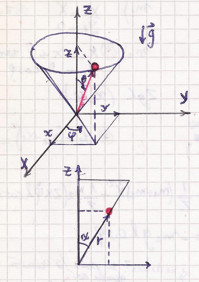
\includegraphics[scale=0.35]{images/fig_mc_problema_cono.jpg}

En este problema convienen esféricas $\theta$ constante. Tendremos dos grados de libertad $(\varphi,r)$.
Usando las expresiones de las coordenadas esféricas (ver XXXX chap 1) se tiene 
\[
	| \dot{\vb{x}} |^2 = | \dot{r}\hat{r} + r\sin\theta \dot{\vp} \hat{\vp} |^2
\]
\[
	v^2 = \dot{r}^2 + r^2 \dot{ \vp }^2 \sin^2 \alpha
\]
Con esto escribimos $T$ usando que $V = mgr\cos\alpha$,
\[
	\Lag = \frac 1 2 m (\dot{r}^2 + r^2 \dot{ \vp }^2 \sin^2 \alpha) - mgr \cos\alpha 
\]

El grado de libertad $\vp$ tendrá asociado un momento conjugado que se conserva, pues $\partial\Lag/\partial \vp = 0$,
luego
\[
	\dpar{\Lag}{\dot{\vp}} = mr^2 \dot{\vp} \sin^2 \alpha = cte. \equiv L
\]
mientras la ecuación de E-L para $r$ arrojará
\[
	m\ddot{r} - m r \dot{\vp}^2 \sin^2\alpha + mg\cos\alpha = 0
\]
y utilizando la conservación 
\[
	\ddot{r} - \frac{L^2}{mr^3\sin^2\alpha} + mg\cos\alpha = 0.
\]

Si ahora calculamos la energía $E=T+V$ se obtiene 
\[
	E = \frac 1 2 m \dot{r}^2 + \frac{L^2 \vp}{ m r^2 \sin^2 \alpha } + mgr\cos\alpha
\]
donde los dos últimos términos constituyen un potencial efectivo.
 
\end{ejemplo}

\begin{ejemplo}{\bf Cicloides y esas cosas}
Tautocrona, Huygens (1773)

\subsubsection*{Curva cicloide}

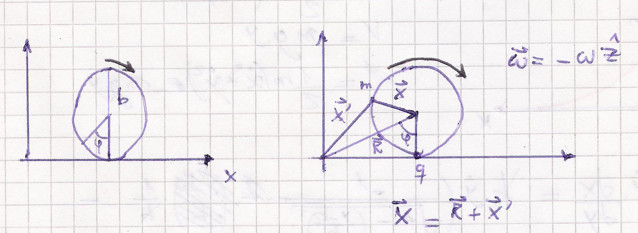
\includegraphics[scale=0.3]{images/fig_mc_cicloides.jpg}

Con las consideraciones de las figuras, tenemos en rápida sucesión
\[
	\vb{R} = (vt,b)
\]
\[
	\vb{X}' = ( -b \sin \vp, -b \cos \vp ) ; \quad \vp = \omega t
\]
\[
	\vb{X} = ( vt -b \sin \vp, b -b \cos \vp )
\]
y por condición de rodadura
\[
	\vb{v}_q = 0 = \vb{v}_{cm} + \vb{\omega} \times \vb{x}_{cm} = v\hat{x} + (-\omega)b\hat{k} \times (-\hat{y})
\]
\[
	0 = (v-\omega b)\hat{x},
\]
o bien $v=\omega b$ e integrando
\[
	vt = \omega t b = \vp b.
\]

Con esto llego a mi ecuación paramétrica para el cicloide
\[
	\begin{cases}  x = b \: (\vp - \sin \vp )\\
		       y = b \: (1 - \cos \vp )
	\end{cases}
\]
Este cicloide tiene gráfico 

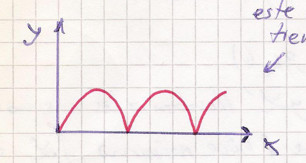
\includegraphics[scale=0.2]{images/fig_mc_cicloide_tiny.jpg}
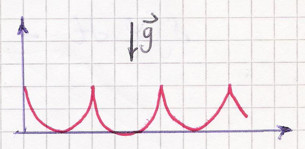
\includegraphics[scale=0.2]{images/fig_mc_cicloide_tiny_inverted.jpg}

Pero neceisto uno que mire hacia abajo, lo cual se logra con un cambio $y' = -y + bz $ de modo que 
\[
	\begin{cases}  x = b \: (\vp - \sin \vp )\\
		       y = b \: (1 + \cos \vp )
	\end{cases}
\]

Ahora se hace un cambio de variables nuevo 
\[
	\frac y b = 1 + \cos\vp \qquad \qquad \frac{y-b}{b} = \cos \vp
\]
y entonces
\[
	x(y) = b \left( \acos\left( \frac{y-b}{b} \right) - \sqrt{1 - ( (y-b)/b )^2} \right)
\]

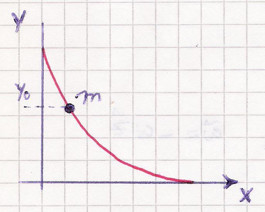
\includegraphics[scale=0.2]{images/fig_mc_cicloide_tobogan.jpg}

Usando todo esto
\[
	T = \frac 1 2 m ( \dot{x}^2 + \dot{y}^2 ) \qquad \qquad V = m g y
\]
\[
	\Lag = \frac 1 2 m ( \dot{x}^2 + \dot{y}^2) - mgy
\]
Derivando $x$ y haciendo el álgebra,
\[
	\dot{x} = -\dot{y} \sqrt{ \frac{ 2b - y }{y} }.
\]

Utilizando toda esta información, el lagrangiano es
\[
	\Lag = \frac{mb\dot{y}}{y} - mgy
\]
y las ecuaciones de E-L
\[
	mb\left( 2\frac{\ddot{y}}{y} - \frac{\dot{y}^2}{y^2} \right) + mg = 0.
\]

Podemos ver, con alguna experiencia, que 
\[
	\dtot{}{t}\left( \frac{ \dot{y}^2 }{y} \right) = \dot{y} \left( 2 \frac{ \ddot{y} }{y} - \frac{\dot{y}^2}{y^2} \right)
\]

Luego,
\[
	m b \frac{1}{\dot{y}} \dtot{}{t}\left( \frac{ \dot{y}^2 }{y} \right) + m g = 0
\]
\[
	\dtot{}{t}\left( \frac{ \dot{y}^2 }{y} \right) = - \frac{ g }{ b } \dtot{y}{t},
\]
y ahora se puede integrar
\[
	\int_0^t \dtot{}{t}\left( \frac{ \dot{y}^2 }{y} \right) dt = 
	- \frac{ g }{ b } \int_0^t \dtot{y}{t} dt,
\]
\[
	\left. \frac{ \dot{y}^2 }{y} \right|_0^t = - \left. \frac{ g }{ b } y \right|_0^t
\]

Usando condiciones iniciales
\[
	\begin{cases}
	 \dot{y}(t=0) = 0 \\
	 y(t=0) = y_0
	\end{cases}
\]
\[
	\frac{ \dot{y}^2 }{ y } = -\frac{ g }{ b } y +  \frac{ g }{ b } y_0
\]
\[
	\dot{y} = \frac{g}{b} \sqrt{ (y_0 - g) y }
\]
de manera que 
\[
	\int_{y_0}^{y} \frac{ dy }{ \sqrt{ y_0y - y^2 } } = \sqrt{ \frac g b } \int_0^t dt = \sqrt{ \frac g b } t
\]
\[
	\asen\left( \frac{ y - y_0/2 }{y_0/2} \right)|_{y_0}^y = \asen\left( \frac{y - y_0/2}{y_0/2} \right)  - \frac \pi 2
\]
\[
	\frac{y - y_0/2}{y_0/2} = \sin ( \sqrt{ \frac g b } t + \pi/2 ) = \cos ( \sqrt{ \frac g b } t )
\]
Finalmente,
\[
	y(t) = \frac {y_0} 2 ( 1 + \cos ( \sqrt{ \frac g b } t ) ).
\]

Si quiero calcular el tiempo de caída será:
\[
	0 = \frac{y_0}{2}\left( 1 + \cos ( \sqrt{ \frac g b } \tau ) \right),
\]
de lo cual se deduce 
\[
	\tau = \sqrt{ \frac b g } \pi.
\]

La cicloide es la curva de caída por la cual se tarda el tiempo mínimo. La masa $m$ tarda lo mínimo en caer por esta curva.
Si las dos ruedas están pegadas girando ambas, recorrerán en un giro una distancia verde:

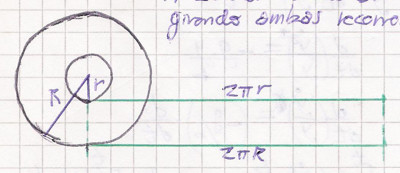
\includegraphics[scale=0.2]{images/fig_mc_ruedas_pegadas.jpg}

Esto no sucede: alguna de ambas deslizará.
\end{ejemplo}




% =================================================================================================
\section{Aplicaciones del principio de acción mínima}
% =================================================================================================

\notamargen{Me falta algo de esta clase inicial, pero esperamos que no sea fundamental!}
El principio variacional de Hamilton tiene más uso como herramiento formal de lo que tiene en el campo de la aplicación.

\[
	S = \int (T-V_0) dt
\]
donde el lagrangiano es con $V=V_0$ constante (un lagrangiano sujeto a potencial constante).
La integral de acción da una medida de la longitud de la órbita (el espacio recorrido).
Para una partícula sujeta a $V=0$
\[
	S = \frac{1}{2}\int m v_0^2 dt = \frac{1}{2}mv_0^2(t-t_0)
\]
de manera que $v_0(t-t_0)$ representa la distancia $d$ recorrida, y es 
\[
	S = \frac{1}{2}mv_0 d
\]

Comentario sobre el cálculo de las variaciones
\notamargen{Esta idea debe estar en el suplemento matemático que le dedicaremos a variacional}
\[
	I = \int f\left(x, \dtot{x}{t}, t\right) dt 
\]
entonces $I$ es extremo si
\[
	\frac{d}{dt} \left( \dpar{f}{[dx/dt]}\right) - \dpar{f}{x} = 0
\]
También podemos encontrar esta notación, dependiendo del tipo de problema,
\[
	I = \int f\left(y, \dtot{y}{x}, x\right) dx 
\]

\subsection{Billares [otro título?]}

Consideramos una partícula libre en una región del espacio (una partícula rebotando en cierta región). Podemos pensar en un
potencial 
\[
	V(\vb{x}) = \begin{cases}
	0\phantom{\infty} \quad \vb{x} \in D \\
	\infty\phantom{0} \quad \vb{x} \notin D
	\end{cases}
\]
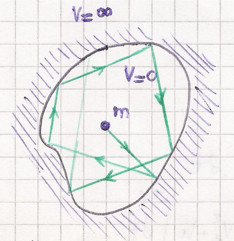
\includegraphics[scale=0.3]{images/fig_mc_billar_1.jpg}

Es un pozo de potencial con una partícula libre en su interior; se los suele llamar {\it billares}. En este caso
\[
	I = \int_{q_i}^{qa_f} \: \Lag( q_1(t), q_2(t), ..., q_k(t),\dot{q}_1(t), ..., \dot{q}_k(t), t ) dt.
\]
La integral da la longitud de la órbita (espacio recorrido)
\[
	\frac 1 2 m v_0^2 \int_{t_i}^{t_f} dt = \frac 1 2 m v_0^2 (t_f - t_i)
\]

En un billar circular 

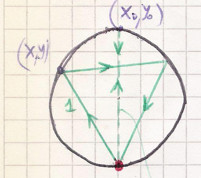
\includegraphics[scale=0.3]{images/fig_mc_billar_2.jpg}
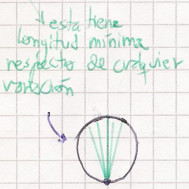
\includegraphics[scale=0.3]{images/fig_mc_billar_2b.jpg}

Si parto del punto rojo y quiero minimizar (extremar) la trayectoria que me da el ir hacia $(x,y)$ y volver al punto rojo, obtendré
una órbita periódica en $(x_0,y_0)$. Esa órbita periódica es extrema entre ir y volver al punto rojo.

En un billar eliptico

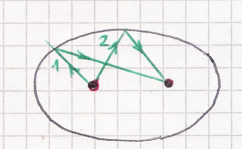
\includegraphics[scale=0.3]{images/fig_mc_billar_3.jpg} 

hay muchas trayectorias posibles entre los focos.
El lagrangiano integrado me da todos las extremas $(1,2,...)$, que por otro lado son las reales, y con las condiciones iniciales determinaré qué 
trayectoria extrema estaré considerando.

Hay muchas trayectorias $(1,2,...)$ que son posibles 

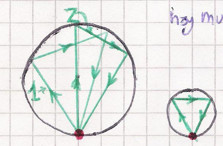
\includegraphics[scale=0.3]{images/fig_mc_billar_4.jpg} 

\[
	I = \int \Lag
\]
da la longitud total de todo el camino.
\notamargen{¿Esta sección aporta algo?}


\subsection{Minimización del camino entre dos puntos}

\notamargen{Esto lo clavo por acá, después reacomodarlo}

\begin{figure}[htb]
	\begin{center}
	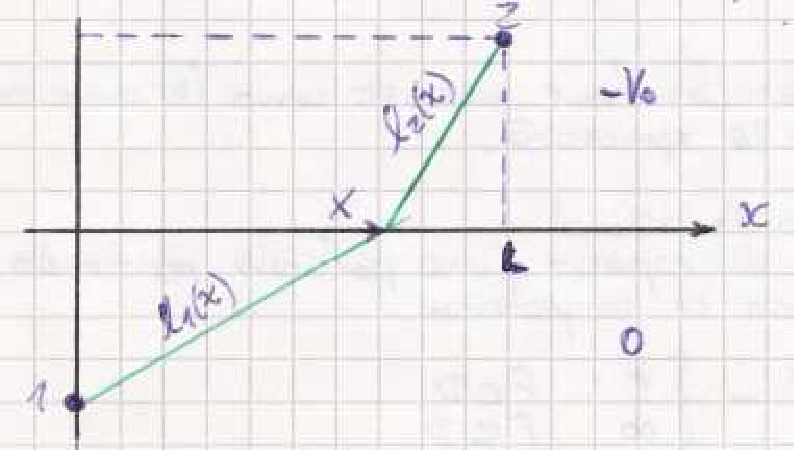
\includegraphics[width=0.4\textwidth]{images/fig_mc_snell1.pdf}	 
	\end{center}
	\caption{}
	\label{fig_mc_snell1}
\end{figure}

El $ \tau $ es fijo.
Este problema no es como el del billar porque la velocidad no es constante [?].
\[
	I = \int_1^2 \Lag \: dt 
\]
pero se puede descomponer en $ I = I_1 + I_2 $; es decir un lagrangiano para cada medio, luego
\[
	I = \frac{1}{2} m v_1^2 \int_0^{t_i} dt + (\frac{1}{2} m v_2^2 + V_0) \int_{t_i}^{t_f} dt ,
\]
que al integrar da
\[
	I = \frac{1}{2} m v_1^2 t_i + \frac{1}{2} m v_2^2( t_f - t_i ) + V_0( t_f - t_i ).
\]

Las condiciones geométricas del problema (ver Figura) implican que 
\[
	v_1 t_i = \ell_1(x) \qquad \qquad v_2 ( t_f - t_i ) = \ell_2(x)
\]
siendo $ \ell_i $ longitudes que dependen de $ x $. Esto permite expresar los tiempos $t$ en términos
de la distancia $ x $ sobre la frontera. Entonces se obtiene la acción $I$ en términos de posiciones
y velocidades, i.e.
\[
	I = I(v_1,v_2 ,x) = \frac{1}{2} m v_1 \ell_1(x) + \frac{1}{2} m v_2 \ell_2(x) + \frac{V_0}{V_2} \ell_2(x).
\]

Luego, como todo sucede a $\tau$ fijo ($t_f=\tau$) se debe tener el siguiente vínculo
\[
	\tau = \frac{\ell_1(x)}{v_1} + \frac{\ell_2(x)}{v_2}.
\]
Entonces, diferenciando implícitamente el vínculo y la integral $I$ obtenemos, respectivamente,
\[
	d\tau = 0 = \left( \frac{1}{v_1} \dtot{\ell_1}{x} + \frac{1}{v_2} \dtot{\ell_2}{x} \right) dx
	-\frac{\ell_1}{v_1^2} dv_1 - \frac{\ell_2}{v_2^2}dv_2
\]
\[
	dI = \left(  \frac{v_1}{2} \dtot{\ell_1}{x} +  \frac{v_2}{2} \dtot{\ell_2}{x} + 
	 \frac{V_0}{v_2} \dtot{\ell_2}{x} \right) dx + 
	\frac{\ell_1}{2} dv_1 + \left( \frac{\ell_2}{2} - \frac{V_0 \ell_2}{v_2^2} \right)dv_2 = 0
\]
En esta última ecuación, si fuesen independientes los diferenciales $dx,dv_1,dv_2$ entonces sería nulo cada
paréntesis. Como no es el caso empleamos multiplicadores de Lagrange,
\[
	d\tau = \lambda \left( \frac{1}{v_1} \dtot{\ell_1}{x} + \frac{1}{v_2} \dtot{\ell_2}{x} \right) dx
	- \lambda \frac{\ell_1}{v_1^2} dv_1 - \lambda \frac{\ell_2}{v_2^2}dv_2
\]
y combinando
\begin{multline*}
 	\left(  \frac{v_1}{2} \dtot{\ell_1}{x} +  \frac{v_2}{2} \dtot{\ell_2}{x} + 
	 \frac{V_0}{v_2} \dtot{\ell_2}{x} - \lambda \left[ \frac{1}{v_1} \dtot{\ell_1}{x} + \frac{1}{v_2} 
	\dtot{\ell_2}{x}  \right] \right) dx + \\
	\left( \frac{\ell_1}{2} + \lambda \frac{\ell_1}{v_1^2} \right) dv_1 + 
	\left( \frac{\ell_2}{2} - \frac{V_0 \ell_2}{v_2^2} + \lambda \frac{\ell_2}{v_2^2} \right)dv_2.
\end{multline*}

Ahora se puede igualar a cero cada paréntesis porque consideramos independientes $v_1$ y $v_2$.
Entonces, se tienen
\[
	\lambda = -\frac{1}{2}v_1^2 \qquad \qquad \lambda = -\frac{1}{2}v_2^2 + V_0
\]
de manera que ha resultado la conservación de la energía
\[
	\frac{1}{2}v_1^2 = \frac{1}{2}v_2^2 - V_0
\]

Reemplazando en la anterior expresión, se llega a
\[
	v_1 \dtot{\ell_1}{x} + v_2 \dtot{\ell_2}{x} = 0.
\]

\[
	\ell_1 = \sqrt{ Y_0^2 + x^2 } \qquad \ell_2 = \sqrt{ Y_f^2 + (L-x)^2 }
\]
\[
	\dtot{\ell_1}{x} = \sin(\alpha_1) \qquad \dtot{\ell_2}{x} = -\sin(\alpha_2)
\]
de modo que 
\[
	v_1 \sin( \alpha_1 ) = v_2 \sin( \alpha_2 ),
\]
que es la conclusión de la ley de Snell. Entonces podemos establecer un parangón entre mecánica clásica
y óptica geométrica.

\begin{figure}[htb]
	\begin{center}
	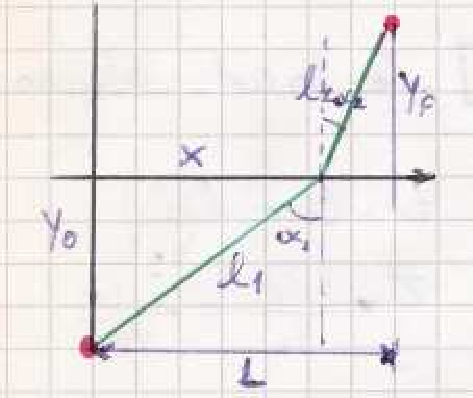
\includegraphics[width=0.4\textwidth]{images/fig_mc_snell2.pdf}	 
	\end{center}
	\caption{}
	\label{fig_mc_snell2}
\end{figure}



% =================================================================================================
\section{Multiplicadores de Lagrange}
% =================================================================================================

El principio variacional de Hamilton nos dice que la trayectoria real que sigue un sistema es la que 
extremiza la acción
\[
	S = \int_{t_i}^{t_f} \Lag \left( q_i[t], \dot{q}_i[t], t \right) dt.
\]
\notamargen{Habría que tomarse medio minuto para chequear: consistencia de la notación con respecto a los límites
en estas integrales de acción, definir extremización, ver si la implicancia es un sí y sólo sí o no, etc.}
Esa condición de extremo, conducía directamente a las ecuaciones de Euler-Lagrange, es decir
\be
	\delta S = 0 \quad \Leftrightarrow \quad \int \sum_{j=1}^{N} 
	\left[ \frac{d}{dt}\left( \dpar{\Lag}{\dot{q}_j} \right) - \dpar{\Lag}{q_j} \right]\delta q_j \: dt = 0
	\label{accion_nula_ecsel}
\ee
donde $\delta q_j$ eran desplazamientos independientes y esta condición significaba que el corchete debía
ser nulo para todo grado de libertad $j$.

Pero puede suceder (en el caso de vínculos no-holónomos, por ejemplo) que no se pueda despejar alguna $ q_j $ y 
entonces no todos los  $\delta q_j$ son independientes.

Si se tienen $s$ ecuaciones de vínculo no holónomos [¿cómo es un vínculo no-holónomo? o es que se deriva una
ecuación de vínculo usual??]
% y se las deriva con respecto al tiempo obtenemos
\[
	\sum_{\ell}^N a_\ell^k(q_i,t) \dot{q}_\ell + b^k(q_i,t) = 0 \qquad \qquad k=1,2,...,s
\]
donde $\ell$ suma en los grados de libertad.
% que son los vínculos ($k=1,...,s$); son $s$ ecuaciones de vínculo.
Multiplicando por $\delta t$ puede verse que no son independientes,
\[
	\sum_{\ell}^N a_\ell^k(q_i,t) \delta {q}_\ell + b^k(q_i,t) \delta t= 0 .
\]

Si ahora las $\delta q_\ell$ son variaciones a $t$ fijo, entonces se cumple 
\[
	\sum_{\ell}^N a_\ell^k(q_i,t) \delta {q}_\ell = 0,
\]
expresión que puede intregrarse con respecto al tiempo y sumar sobre todas las ecuaciones de vínculo,
\[
	\sum_{k}^s \int_{t_i}^{t_f} \lambda^k \sum_{\ell}^N a_\ell^k(q_i,t) \delta {q}_\ell \: dt = 0.
\]

El cero de esta última ecuación puede restarse del otro cero dado por la integral \eqref{accion_nula_ecsel},
suma de $N-s$ ecuaciones con $\delta q_\ell$ independientes [¿checar esto?] con para construirnos de esa manera la ecuación
% Podemos sacar la suma fuera,
% \[
% 	\sum_{k}^s \int_{t_i}^{t_f} \lambda^k \sum_{\ell}^N a_\ell^k(q_i,t) \delta {q}_\ell dt = 0
% \]
% Absorbo la otra sumatoria en el segundo término y paso de $\ell \to j$.
\[
	\int \sum_{j=1}^{N-s} \left\{ \frac{d}{dt}\left( \dpar{\Lag}{\dot{q}_j} \right) -\dpar{\Lag}{q_j}
	- \sum_{k}^s \lambda^k a_j^k(q_i,t) \right\} \delta {q}_j \: dt = 0
\]
y se tienen $N-s$ ecuaciones
\[
	\frac{d}{dt}\left( \dpar{\Lag}{\dot{q}_j} \right) -\dpar{\Lag}{q_j} =  \sum_{k}^s \lambda^k a_j^k(q_i,t),
\]
y $s$ ecuaciones 
\be
	\sum_{\ell}^N a_\ell^k(q_i,t) \dot{q}_\ell + b^k(q_i,t) = 0 .
	\label{ecs_vinculo}
\ee

El parámetro $ \lambda^k $ es la fuerza de vínculo asociada al vínculo que no se pudo despejar. Es un multiplicador de
Lagrange.

Los vínculos holónomos se pueden escribir también en la forma \eqref{ecs_vinculo}. Un vínculo holónomo está representado
por una ecuación del tipo 
\[
	f( \vb{x}_1, \vb{x}_2, ...,\vb{x}_N, t ) = cte.
\]
de manera que para desplazamientos virtuales (donde $\delta t=0$) la derivada temporal de esta ecuación implica\footnote{Recordemos
que para desplazamientos virtuales el término $\partial f /\partial t$ no aparece por estar multiplicado a $\delta t=0$.} 
\[
	\sum_i \nabla_i f \cdot \delta\vb{x}_i = 0
\]
y esta ecuación es precisamente de la forma $ \sum_\ell a_\ell^k \delta q_\ell $.
\notamargen{Falta entender bien principio trabajos virtuales y despl virtual ($\delta t=0$)}

% ~~~~~~~~~~~~~~~~~~~~~~~~~~~~~~~~~~~~~~~~~~~~~~~~~~~~~~~~~~~~~~~~~~~~~~~~~~~~~~~~~~~~~~~~~
% ~~~~~~~~~~~~~~~~~~~~~~~~~~~~~~~~~~~~~~~~~~~~~~~~~~~~~~~~~~~~~~~~~~~~~~~~~~~~~~~~~~~~~~~~~
\begin{ejemplo}{\bf Resolución de sistema holónomo}

Consideramos un cilindro rodando sin deslizar.
\notamargen{Aclarar mil cosas: rueda un poco (máximo $\alpha = pi/2 $). ¿Es una aproximación sólo válida para
ángulos pequeños? El caso exacto es mucho quilombo? Sirve para algo?}

Los vínculos son relaciones entre velocidades que se pueden intergrar.
De la soga:
\[
	\dot{x}_1 + \dot{\alpha} a = \dot{x}_2
\]
por el rozamiento sobre el piso:
\[
	\dot{\alpha} a = \dot{x}_1
\]
\notamargen{Lo de los $\delta$ pide para ser explicado y entendido.}
\[
	\Delta x_1 + a \Delta \alpha = \Delta x_2
	\qquad \qquad 
	\Delta \alpha a = \Delta x_1
\]
\[
	\delta x_1 + a \delta \alpha - \delta x_2 = 0
	\qquad \qquad \delta x_1 - a \delta \alpha = 0 
\]
El lagrangiano es
\[
	\Lag = \frac{1}{2} m \dot{x}_2^2 + \frac{1}{2}M\dot{x}_1^2 + \frac{1}{2}I\dot{\alpha}^2 + mgx_2
\]
donde los dos términos centrales en el rhs son la cinética del cuerpo rígido.

Ahora hacemos 
\[
	\lambda^1 ( \delta x_1 + a \delta \alpha - \delta x_2 ) = 0 \qquad \qquad 
	\lambda^2 ( \delta x_1 - a \delta \alpha ) = 0
\]
donde deberíamos obtener $ \lambda^1 $ tensión y $ \lambda^2 $ fuerza de rozamiento.
Luego,
\begin{eqnarray*}
	m\ddot{x}_1 & = (\lambda^1 1 + \lambda^2 1) \\
	m\ddot{x}_2 & = mg + \lambda^1(-1) \\
	I\ddot{\alpha} & = (\lambda^1 a - \lambda^2 a)
\end{eqnarray*}

Escribiendo las ecuaciones de Newton para este problema resulta en
\begin{eqnarray*}
	m\ddot{x}_1 & = T - F_{\text{roz}} \\
	m\ddot{x}_2 & = mg - T \\
	I\ddot{\alpha} & = T a + F_{\text{roz}} a 
\end{eqnarray*}
de manera que identificamos naturalmente a 
\[
	\lambda^1 = T \qquad \qquad \lambda^2 = - F_{\text{roz}}
\]
% ~~~~~~~~~~~~~~~~~~~~~~~~~~~~~~~~~~~~~~~~~~~~~~~~~~~~~~~~~~~~~~~~~~~~~~~~~~~~~~~~~~~~~~~~~
% ~~~~~~~~~~~~~~~~~~~~~~~~~~~~~~~~~~~~~~~~~~~~~~~~~~~~~~~~~~~~~~~~~~~~~~~~~~~~~~~~~~~~~~~~~
\end{ejemplo}

Entonces, para el caso de vínculo holónomos tendremos $ a^k_\ell(q_i,t) = \nabla_i f^k \cdot \delta \vb{x}_i $ de modo que
\[
	\frac{d}{dt}\left( \dpar{\Lag}{\dot{q}_j} \right) -\dpar{\Lag}{q_j} =
	\sum_{k}^s \lambda^k \: \dpar{f^k}{q_j}
	\label{ecs_el_vinculos}
% 	\nabla_j f^k \cdot \frac{\delta \vb{x}_j}{\delta q_j}
\]
\notamargen{Hay que escribir bien la conversión de $\nabla f^k$ hacia $\partial f^k / \partial q_j $. Parece una boludez,
pero tal vez no sea así.}

Pero sabemos [sí?] que cuando existe fuerza generalizada (no proveniente de un potencial) se tenía 
\be
	\frac{d}{dt}\left( \dpar{\Lag}{\dot{q}_j} \right) -\dpar{\Lag}{q_j} = Q_j, \qquad \qquad 
	Q_j = \sum_i^N \vb{F}_i^a \cdot \dpar{\vb{x}_i}{q_j}
	\label{ecs_el_fuerza_generalizada}
\ee
% siendo $\nabla_j f^k $ el gradiente de la ecuación de víngulo respeco de $j$ y 
e igualando los miembros derechos de \eqref{ecs_el_vinculos} y \eqref{ecs_el_fuerza_generalizada} 
\[
	\sum_i^N \vb{F}_i^a \cdot \dpar{\vb{x}_i}{q_j} = \sum_{k}^s \lambda^k \: \dpar{f^k}{q_j}
\]
se arriba a que 
\notamargen{Acá hay temas con los índices y con lo que se suma. Parece no ser la misma cosa.}
\[
	\lambda^k = \vb{F}_i^a 
\]
de manera que $\lambda^k$ son las fuerzas de vínculo asociadas a los vínculos que no se pudieron retirar
(no despejados en las ecuaciones [?]).
Si los vínculos son holónomos (pero no quise despejar) entonces son las fuerzas de vínculo.

La moraleja es que si no puedo despejar en función de coordenadas independientes sí o sí necesito introducir
multiplicadores de Lagrange.

Tenía anotado que \eqref{ecs_el_fuerza_generalizada} es el lagrangiano con fuerzas no conservativas, cuando por 
supuesto $\vb{F}$ son fuerzas no conservativas.


\subsubsection{Más sobre el asunto de vínculos}
\notamargen{Hay que revisar bien esta sección y meter algún ejemplo esclarecedor.}

comparando vemos que 
\[
	Q_j = \sum \lambda^k a^k_j(q_j,t) \quad \textrm{vínculos no holónomos}
\]
\[
	Q_j=  \sum \lambda^k \nabla_j f^k \cdot \delta \vb{r}_j  \quad \textrm{vínculos holónomos}
\]

En el caso de vínculos holónomos 
\[
	g(\vb{r}_1,...,\vb{r}_n,t) = 0 
\]
donde no quise despejar en función de $q_q,...,q_n$ resulta que 
\notamargen{El supraíndice con $\delta q_j$ va sobre el igual en realidad.}
\[
	Q_j^{\delta q_j} =  \sum_i^N \lambda (\nabla_i f^k\cdot\delta\vb{r}_i)
\]
donde $\delta\vb{r}_i$ es un desplazamiento virtual de la partícula.
Vamos a reescribir este término,
\[
	\sum_i^N \dpar{g^k}{\vb{r}_i} \delta \vb{r}_i = 0
\]
\[
	\nabla_i f^k\cdot\delta\vb{r}_i = \sum_i \dpar{g^k}{\vb{r}_i} \dpar{\vb{r}_i}{q_j} \delta q_j
\]
\[
	Q_j^{\delta q_j} =  \lambda \sum_k \dpar{g^k}{\vb{r}_i} \sum_j \dpar{\vb{r}_i}{q_j} \delta q_j
\]
luego como 
\[
	a^k_j \equiv \dpar{g^k}{\vb{r}_i}
\]
se sigue que los $\lambda^k$ son las fuerzas de vínculo.

En el caso de vínculos no holónomos $\lambda^k$ son las fuerzas de vínculo asociadas a los 
vínculos no retirados.

\[
	Q_j {\delta q_j} =  \sum \lambda^k (\nabla_i g^k\cdot\delta\vb{r}_i)
\]
\[
	Q_j =  \sum_k \lambda^k \dpar{g^k}{\vb{r}_i} \dpar{\vb{r}_i}{q_j}
\]
\[
	Q_j =  \sum_k \lambda^k \dpar{g^k}{q_j}
\]
entonces $\lambda^k=F^v$.

Como extra escribamos que para cada grado de libertad $j$ 
\[
	\dpar{\Lag}{q_j} - \frac{d}{dt}\left( \dpar{\Lag}{\dot{q}_j} \right) - \sum_k^s \lambda^k a_j^k \equiv 0
\]
donde $\delta q_j$ son ahora independientes.
\[
	Q_j = \sum_i^N F_i^a \dpar{\vb{r}_i}{q_j}. 
\]

\begin{ejemplo}{\bf Moneda rodando por un plano}

Consideramos una moneda que rueda libremente por un plano (no sujeta a potencial).
Situraemos un sistema de ejes sobre la moneda, que etiquetaremos 123 y otro fijo fuera
de la misma xyz.
\[
	\vb{V}_{cm} = -\vb{\Omega} \times \vb{r} =
	-(\dot{\phi}\hat{2} + \dot{\psi}\hat{3}) \times (-a\hat{2})
\]
\[
	\dot{x}\hat{x} + \dot{y}\hat{y} = -a \dot{\psi}\hat{1}
\]
siendo los vínculos
\[
	z_{cm} - a = 0 \qquad \theta=\pi/2 \qquad |\vb{V}_{cm}| = a\dot{\psi}
\]
de tal modo que son dos grados de libertad. El lagrangiano puede escribirse como 
\[
	\Lag = T = \frac{1}{2}m a^2 \dot{\psi}^2  + \frac{1}{2} I_2^2 \dot{\phi}^2 + \frac{1}{2} I_3^2\dot{\psi}^2.
\]
\notamargen{No entiendo/recuerdo lo que quise decir con la expresión {\it bajar los ejes}.
Calculo que se relaciona con la proyección de los ejes 123 en xyz. Confirmarlo.}

\begin{figure}
	\begin{center}
	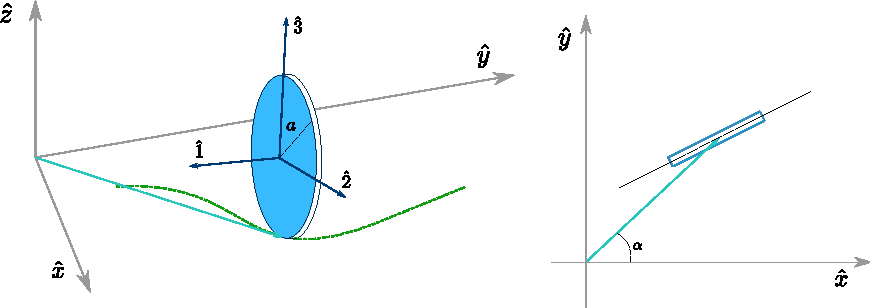
\includegraphics[width=1.0\textwidth]{images/fig_moneda.pdf}	 
	\end{center}
	\caption{Moneda que rueda libremente por un plano. Intercambié ejes 2 y 3 respecto del dibujo anterior.}
\end{figure} 

Como los vínculos dependen de la velocidad, resulta 
\[
	\dot{y} = a\dot{\psi} \cos(\psi) \sin(\phi) = a \sin(\phi) \dot{\psi}
\]
\[
	\dot{x} = a\dot{\psi} \cos(\psi) \cos(\phi) = a \cos(\phi) \dot{\psi}
\]
de tal manera que 
\[
	\dot{y} - a \sin(\phi) \dot{\psi} = 0 \qquad \dot{x} - a \cos(\phi) \dot{\psi} = 0
\]
y luego esto equivale a 
\[
	\lambda_1(dy - a \sin(\phi) d\psi) = 0 \qquad \lambda_2(dx - a \cos(\phi) d\psi)= 0
\]
y finalmente 
\[
	\frac{d}{dt}\left(\dpar{\Lag}{\dot{q}_i}\right) - \dpar{\Lag}{q_i} =
	\lambda_i \nabla_i f \cdot \delta \vb{r}_i
\]
Podemos escribir
\[
	m \ddot{x} = \lambda_1 \qquad m \ddot{x} = m a \frac{d}{dt}( \cos(\phi)\dot{\psi} )
\]
\[
	m \ddot{x} = m a ( -\sin(\phi)\dot{\phi}\dot{\psi} + \cos(\phi)\ddot{\psi} )
\]
\[
	m \ddot{y} = \lambda_2
\]
\[
	I_2\ddot{\phi} = 0 \qquad I_3\ddot{\psi} = - \lambda_2 a \sin(\phi) -\lambda_1 a \cos(\phi)
\]
\[
	\hat{1} = \cos(\psi)[\sin(\phi)\hat{y} + \cos(\phi)\hat{x}]
\]

\label{moneda}
\end{ejemplo}


\subsection{Soluciones aproximadas}

Puedo tomar un subconjunto pequeño de funciones y restringirme a buscar cua es la mejor función de ese conjunto
en el sentido de extremar $I$:
\[
	I = \int_{t_i}^{t_f} \Lag(q_1,...,q_n,\dot{q}_1,...,\dot{q}_n,t) \: dt,
\]
donde el subconjunto de las funciones $q_1,q_2, ... ,q_n$ las tomo de algún subconjunto en particular.
Por ejemplo,
\[
	q_1^f = a_0 + a_1 t_f + ... \qquad q_1^i = a_0 + a_1 t_i + ...
\]

\subsection{Oscilador armónico}

Considero un oscilador armónico en una dimensión.
\[
	\Lag = \frac{1}{2} m \dot{x}^2 - \frac{1}{2} k \dot{x}^2
\]

Quiero resolver de manera aproximada el oscilador armónico y ver que está bien.
Si considero $ n \to \infty $ tengo infinitos parámetros y puedo parametrizar cualquier curva que una los puntos
inicial y final.

\begin{figure}
	\begin{center}
	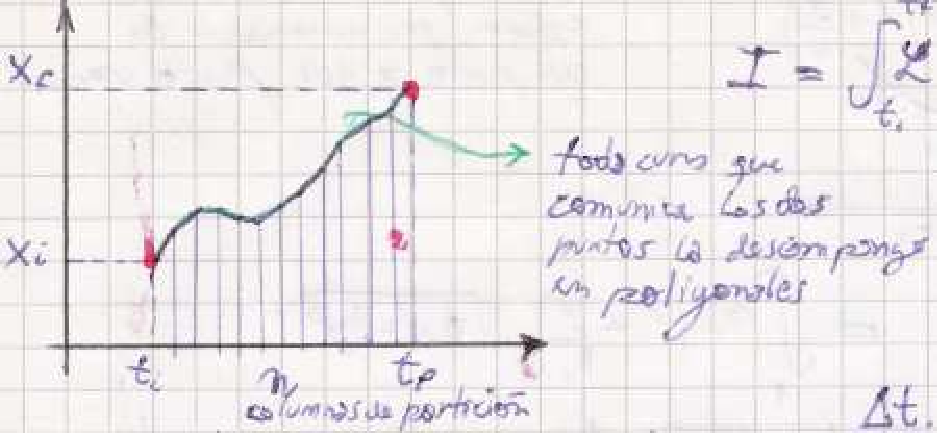
\includegraphics[scale=0.5]{images/fig_mc_oscarm_approx.pdf}	 
	\end{center}
	\caption{}
	\label{fig_mc_oscarm_approx}
\end{figure} 

\notamargen{
comments del gráfico: toda curva que comunica los dos puntos la descompongo en poligonales. Columnas de partición
}

\[
	I = \int_{t_i}^{t_f} \Lag(x,\dot{x}) \: dt
\]
Parto el intervalo y considero una partición de $N$ {\it cachos}.
\[
	\Delta t N = t_i - t_f
\]
donde $\Delta t \to 0$ y $N \to \infty $. Luego la versión discreta de la integral es 
\[
	I \approx \sum_{i=1}^{N-1} \left( \frac{1}{2}m \frac{(x_{i+1} - x_i)^2}{\Delta t^2} 
	- \frac{1}{2} k x_i^2 \right) \Delta t
\]

Tomamos la derivada
\[
	\dpar{I}{x_j} = \left( m \frac{(x_j - x_{j-1})}{\Delta t^2} - m \frac{(x_{j+1} - x_j)}{\Delta t^2} \right) 
	\Delta t - kx_j \Delta t
\]
e igualándola a cero,
\[
	\frac{m}{\Delta t^2} ( -2x_j + x_{j-1} + x_{j+1}) + k x_j = 0
\]
\notamargen{Creo que se puede usar que uno conoce diferencias finitas algo.
El final parece no estar muy claro en la carpeta. Hacer la cuenta a mano bien.}
que se puede escribir como 
\[
	\frac{m}{\Delta t}\left( \frac{x_{j+1} - x_j}{\Delta t} - \frac{x_j - x_{j-1}}{\Delta t} \right) + k x_j = 0
\]
y que en el límite continuo va a 
\[
	m\ddot{x} - kx = 0.
\]



\begin{ejemplo}{\bf Geodésicas}
\notamargen{Este material es parte de una clase práctica. Habría que ver de hacerlo encajar mejor.}
% \section{Geodésicas}
La idea es extremizar la distancia entre dos puntos de una dada geometría.
En el caso del plano se tiene 
\[
	I = \int ds = \int \sqrt{ dx^2 + dy^2 } = \int \sqrt{ 1 + \dot{y}^2 } \; dx
\]
donde se ha definido $\dot{y} \equiv dy/dx$. Evidentemente si la geometría es plana,
la curva que extremiza el intervalo tiene que ser una recta. Veámoslo.
Las ecuaciones de Euler Lagrange se reducen a:
\[
	\dtot{}{dx}\left( \frac{\dot{y}}{\sqrt{1 + \dot{y}^2 }}\right) = 0,
\]
las cuales nos dicen que 
\[
	\frac{\dot{y}}{\sqrt{1 + \dot{y}^2 }} = C
\]
donde $C$ es una constante. No es difícil ver que esta ecuación lleva a 
\[
	y(x) = C_1 x + C_2
\]
para $C_1, C_2$ constantes. Esta es la ecuación de una recta en el plano.


{\bf Un ejemplo más sofisticado}

Si a una curva $z=z(x)$ como la que se ilustra en la figura se la hace girar en torno al
eje $z$ se tiene una superficie de revolución. Un punto tridimensional en esa superficie
se puede parametrizar en términos de coordenadas cilíndricas $\rho,\theta, z$ según
\[
	\begin{cases}
	x = \rho(z) \: \cos( \theta ) \\ 
	y = \rho(z) \: \sin( \theta ) \\
	z = z
	\end{cases}
\]
donde el hecho de que la superificie es 2D se trasluce en que cada coordenada cartesiana
3D $x,y,z$ depende a lo sumo de dos variables $\theta,z$.

La trayectoria mínima entre dos puntos provendrá otra vez de extremar
\[
	I = \int ds = \int \sqrt{ dx^2 + dy^2 + dz^2 }
\]
pero utilizando la restricción de la superficie dada por las ecuaciones XXX. Utilizando
la prima para denotar la derivada con respecto a $z$ se tiene 
\[
	dx = \rho' \cos \theta dz - \rho \sin \theta d\theta
\]
\[
	dy = \rho' \sin \theta dz + \rho \cos \theta d\theta
\]

\[
	I = \int \sqrt{ {\rho'}^2 dz^2 + \rho^2 d\theta^2 + dz^2 }
\]
que se puede poner en términos de la derivada con respecto a $z$ sacando como factor común
su diferencial. Entonces
\[
	I = \int \sqrt{ ( {\rho'}^2 + 1 ) dz^2 + \rho^2 {\theta'}^2 } dz
\]
donde tanto $\rho$ como $\theta$ son funciones de $z$.
El lagrangiano es función de $\theta', \rho, \rho'$

Si calculamos las ecuaciones de Euler Lagrange para $\theta$ (que son las más fáciles puesto que
la dependencia es solo de la derivada) se llega a
\[
	\frac{\rho \rho' \theta' }{\sqrt{ ( {\rho'}^2 + 1) + \rho^2 {\theta'}^2 }} = C
\]
que se puede, haciendo el álgebra correspondiente, lleva a la forma explícita
\be
	\theta(z) = C_1 \int \frac{\sqrt{ {\rho'}^2 + 1 }}{ 2 \sqrt{ \rho^2 - C_1^2 } } dz + C_2,
	\label{ec_sup_rev}
\ee
que es una ecuación genérica para una superficie en rotación. Es decir, que recorrer la curva
de longitud mínima por esa superficie debe hacerse avanzando en $\theta$ según la prescripción
dada por \eqref{ec_sup_rev}.

Si la superficie fuera un cilindro, de radio $a$, por ejemplo, se tendría $\rho=a$ de modo que la
\eqref{ec_sup_rev} se integra inmediatamente para dar 
\[
	\theta(z) = C_1 \frac{z}{ a \sqrt{ a^2 - C_1^2 } } .
\]
Luego, para dos puntos separados verticalmente una distancia $h$ (ver figura) sobre la superficie
del cilindro se tiene que la curva que representa la distancia mínima es una hélice en el cilindro,
de paso $h$. Si la superficie lateral de este cilindro se desplegase sobre un plano, esa curva es
una recta.

{\bf Superficie general en 3D}

Si la partícula debe {\it caminar} en la superficie $\Omega$ entonces tal vez se pueda expresar
como $z=z(x,y)$ de tal forma se tendrá
\[
	I = \int f(\dot{x},\dot{y},\dot{z}) dt
\]
Luego, la derivada total de $z$ será
\[
	\dtot{z}{t} = \dot{z} = \dpar{z}{x} \dot{x} + \dpar{z}{y} \dot{y}
\]
y entonces 
\[
	I = \int f(\dot{x},\dot{y},\dpar{z}{x} \dot{x} + \dpar{z}{y} \dot{y}) dt.
\]

Planteando las ecuaciones de Euler-Lagrange 
\[
	\dtot{}{t}\left( \dtot{f}{\dot{x}} + \dtot{f}{\dot{z}}\dtot{z}{x} \right) -
	\dtot{f}{\dot{z}}\dtot{}{x}
	\left( \dpar{z}{x} \dot{x} + \dpar{z}{y} \dot{y} \right) = 0
\]
\[
	\dtot{}{t}\left( \dtot{f}{\dot{y}} + \dtot{f}{\dot{z}}\dtot{z}{y} \right) -
	\dtot{f}{\dot{z}}\dtot{\dot{z}}{y} = 0
\]
las cuales se pueden simplificar usando la derivada total,
\[
	\dtot{}{t}\left( \dtot{f}{\dot{x}} \right) + \dtot{}{t}\left( \dtot{f}{\dot{z}} \right)
	\dtot{z}{x} + \dtot{f}{\dot{z}}\dtot{}{t}\left( \dtot{z}{x} \right) + 
	\dtot{f}{\dot{z}}\dtot{}{t}\left( \dtot{z}{x} \right) = 0
\]
\notamargen{Los dos últimos términos tienen que aparecer tachados.}

Luego,
\[
	\dtot{}{t}\left( \dtot{f}{\dot{x}} \right) + 
	\dtot{z}{x}\dtot{}{t}\left( \dtot{f}{\dot{z}} \right) = 0
\]
\[
	\dtot{}{t}\left( \dtot{f}{\dot{y}} \right) + 
	\dtot{z}{y}\dtot{}{t}\left( \dtot{f}{\dot{z}} \right) = 0
\]
y como
\[
	\dtot{G}{x}\dot{x} + \dtot{G}{y}\dot{y} + \dtot{G}{z}\dot{z} = 0,
\]
se sigue que 
\[
	\dot{z} = -\left( \dtot{G}{x}\dot{x} + \dtot{G}{y}\dot{y} \right) \frac{1}{dG/dz}
\]
o bien
\[
	\dot{z} = -\left( \frac{G_x}{G_z}\dot{x} + \frac{G_y}{G_z}\dot{y} \right)
\]
de tal manera que 
\[
	\dtot{}{t}\left( \dtot{f}{\dot{x}} \right) + 
	\frac{G_x}{G_z}\dtot{}{t}\left( \dtot{f}{\dot{z}} \right) = 0
\]
\[
	\dtot{}{t}\left( \dtot{f}{\dot{y}} \right) + 
	\frac{G_y}{G_z}\dtot{}{t}\left( \dtot{f}{\dot{z}} \right) = 0
\]
\[
	\dtot{}{t}\left( \dtot{f}{\dot{z}} \right) = \lambda(t) G_z
\]

Entonces
\[
	\frac{1}{G_x} \dtot{}{t}\left( \dtot{f}{\dot{x}} \right) = 
	\frac{1}{G_y} \dtot{}{t}\left( \dtot{f}{\dot{y}} \right) = 
	\frac{1}{G_z} \dtot{}{t}\left( \dtot{f}{\dot{z}} \right) 
\]

Esta expresión puede simplificarse como 
\[
	f = \sqrt{ \dot{x}^2 + \dot{y}^2 + \dot{z}^2 } = 1
\]
si el parámetro $t$ es $s$
\[
	s = \int ds = \int \sqrt{dx^2 + dy^2 + dz^2 } =
	\int \sqrt{ \dot{x}^2 + \dot{y}^2 + \dot{z}^2 } ds
\]
y entonces
\[
	\dtot{}{t}\left( \dtot{f}{\dot{x}} \right) = \ddot{x}
\]
de manera que la ecuación de la geodésica es
\[
	\frac{1}{G_x}\dtot[2]{x}{s} = \frac{1}{G_y}\dtot[2]{y}{s} = 
	\frac{1}{G_z}\dtot[2]{z}{s}
\]

Ahora, si consideramos
\[
	I = \int [f(\dot{x}, \dot{y}, \dot{z}) + \lambda G(x,y,z)] dt
\]
se tiene que 
\[
	\dtot{}{t}\left( \dtot{f}{\dot{x}}\right) - \lambda G_x = 0
\]
y es un vínculo que hay que integrar, y es mucho más difícil.

Volviendo a la superficie general
\[
	I = \int \left[\frac{1}{2} m (\dot{x}^2 + \dot{y}^2 +
	   \dot{z}^2 ) - \lambda G \right] dt
\]
\[
	T = \sqrt{(\dot{x}^2 + \dot{y}^2 + \dot{z}^2)} = cte. \equiv k
\]
y entonces $s=kt$

\[
	k^2 m \ddot{x} - \lambda G_x = 0
\]
\[
	k^2 m \ddot{y} - \lambda G_y = 0
\]
\[
	k^2 m \ddot{z} - \lambda G_z = 0
\]

\[	
	G(x,y,z) = 0
\]

La partícula se mueve en una geodésica 
\[
	\frac{\ddot{x}}{G_x} = \frac{\ddot{y}}{G_y} = \frac{\ddot{z}}{G_z}
\]
\end{ejemplo}


% =================================================================================================
\section{Potenciales dependientes de la velocidad}
% =================================================================================================

Hasta el momento se consideró que el potencial $V$ dependía únicamente de la posición y resultaba eso en
una fuerza generalizada [la llamé así?]
\[
	Q_j = -\dpar{V}{q_j}
\]
para la cual el $\Lag\equiv T-V$ cumplía las ecuaciones de Euler Lagrange
\be
	\dtot{}{t} \left( \dpar{\Lag}{\dot{q}_j} \right) - \dpar{\Lag}{q_j} = 0.
	\label{el-pot-x}
\ee

Si en cambio se tiene un potencial dependiente, además, de la velocidad,
\[
	U = U(q_1, ..., q_2,\dot{q}_1,...,\dot{q}_n,t ) 
\]
y se requiere que sigan valiendo las ecuaciones \eqref{el-pot-x} para $\Lag \equiv T-U$, necesitaremos evidentemente
\[
	Q_j = \dtot{}{t} \left( \dpar{U}{\dot{q}_j} \right)  -\dpar{U}{q_j},
\]
una fuerza generalizada que depende de posiciones y velocidades.

El ejemplo canónico de una tal fuerza es la fuerza de Lorentz, que es la que sufre una partícula de carga $q$ en
presencia de un campo electromagnético dado por campos $\vb{E}, \vb{B}$ y cuya forma es
\be
	\vb{F} = q \vb{E} + \frac{q}{c} ( \vb{v} \times \vb{B} )
	\label{f_lorentz}
\ee

Esta fuerza \eqref{f_lorentz} puede expresarse en términos de dos potenciales. Para ello es necesario recurrir a
las relaciones que verifican los campos $\vb{E}, \vb{B}$ y que están dadas por las ecuaciones de Maxwell, cuyo esquema 
se presenta en la siguiente tabla.
\begin{center}
\begin{tabular}{|c|c|}
\hline
& \\
$ \nabla\cdot\vb{E} = 4 \pi \rho $ & $ \nabla \cdot \vb{B} = 0 $ \\
& \\
$ \displaystyle \rotorm{E} = -\frac{1}{c} \dpar{\vb{B}}{t} $ &  
$ \displaystyle \rotorm{B} = \frac{4\pi}{c}\vb{J} + \frac{1}{c} \dpar{\vb{E}}{t} $ \\
 & \\
\hline
\end{tabular}
\end{center}

Dado que la divergencia de \vb{B} es nula, entonces existe un potencial vector \vb{A} tal que 
\[
	\rotorm{A} = \vb{B}.
\]
Entonces, la ley de Faraday resulta 
\[
	\rotorm{E} = -\frac{1}{c} \dpar{}{t} \left(\rotorm{A} \right) 
\]
o bien 
\[
	\nabla\times\left( \vb{E} + \frac{1}{c}\dpar{\vb{A}}{t} \right) = 0
\]

La cantidad entre paréntesis es de rotor nulo y entonces se puede escribir
\[
	\vb{E} + \frac{1}{c}\dpar{\vb{A}}{t} = -\nabla \vp( \vb{x}, t )
\]
de manera que los campos \vb{B}, \vb{E} pueden expresarse en términos de una función escalar $\vp$ y un campo vectorial
\vb{A} como
\[
	\vb{B} = \rotorm{A} \qquad \qquad \vb{E} = - \nabla \vp - \frac{1}{c} \dpar{ \vb{A} }{t} .
\]

Entonces, en términos de estos potenciales \eqref{f_lorentz} resulta 
\[
	\vb{F} = -q\nabla \vp - \frac{q}{c} \dpar{ \vb{A} }{t} + \frac{q}{c} \vb{v} \times \rotorm{A}.
\]

Supongamos, para simplificar el razonamiento, que es $ \vb{F} = F_x \hat{x} $ y veamos que 
\[
	F_x = -q \dpar{ \vp }{ x } - \frac{q}{c} \dpar{ A_x }{t} + \frac{q}{c} \left( v_y [\rotorm{A}]_z - v_z [\rotorm{A}]_y \right)
\]
se puede escribir
\[
	F_x = \dtot{}{t} \left( \dpar{U}{v_x} \right)  -\dpar{U}{x}.
\]

Desarrollando explícitamente el rotor se tiene 
\[
	\left( v_y [\rotorm{A}]_z - v_z [\rotorm{A}]_y \right) = 
	v_y \dpar{A_y}{x} - v_y \dpar{A_x}{y} - v_z \dpar{A_x}{z} + v_z \dpar{A_z}{x} + v_x \dpar{A_x}{x} - v_x \dpar{A_x}{x}
\]
donde se ha sumado y restado la conveniente combinación $ v_x \partial_x A_x $. Dado que las velocidades y las posiciones son variables
independientes (se verifica $ \partial_a v_b = 0 $ para cualquier combinación $ a,b=x,y,z $) se puede {\it filtrar} la velocidad dentro
de las derivadas para reescribir 
\[
	v_x \dpar{A_x}{x} + v_y \dpar{A_y}{x} + v_z \dpar{A_z}{x} = \dpar{}{x}( v_xA_x + v_yA_y + v_zA_z ) = \dpar{}{x}( \pe{v}{A} )
\]
% \[
% 	\left( v_y [\rotorm{A}]_z - v_z [\rotorm{A}]_y \right) = 
% 	\dpar{}{x}( v_xA_x + v_yA_y + v_zA_z ) - v_x\dpar{ A_x}{x} - v_y\dpar{A_x}{y} - v_z\dpar{A_x}{z}.
% \]
Los tres términos restantes en derivadas respecto de $A_x$ no son otra cosa que una derivada total,
\[
	- \frac{q}{c} \left(  \dpar{ A_x }{t}- v_x\dpar{ A_x}{x} - v_y\dpar{A_x}{y} - v_z\dpar{A_x}{z} \right) =
	- \frac{q}{c} \left( \dpar{ A_x }{t} - \vb{v}\cdot\nabla( A_x ) \right) = - \frac{q}{c} \dtot{A_x}{t}
\]

Luego, se fuerza la aparición de una derivada con respecto a la velocidad (para obtener una expresión en consonancia con la buscada)
del siguiente modo
\[
	A_x = \dpar{}{v_x}(v_xA_x + v_yA_y + v_zA_z) = \dpar{}{v_x}(\pe{v}{A}),
\]
y juntando todo resulta
% \[
% 	F_x = -q \dpar{ \vp }{ x } - \frac{q}{c} \dpar{ A_x }{t} + \frac{q}{c} \left( \dpar{}{x}( \pe{v}{A} )
% 	- v_i \partial_i\left( \dpar{}{v_x}(\pe{v}{A}) \right) \right)
% % 	- v_x \dpar{}{x}( \dpar{}{v_x}(\pe{v}{A}) ) - v_y \dpar{}{y}( \dpar{}{v_x}(\pe{v}{A}) ) 
% % 	- v_z \dpar{}{z}( \dpar{}{v_x}(\pe{v}{A}) ) \right).
% % 	
% \]
% donde el último término en el RHS representa la suma de tres. Reordenando esta expresión
\[
	F_x = -\dpar{ }{ x }\left( q\vp - \frac{q}{c} \pe{v}{A} \right) 
	+ \dtot{ }{t} \left( \dpar{}{v_x}\left( -\frac{q}{c}\pe{v}{A} \right) \right) .
\]

Como $\vp=\vp(\vb{x},t)$, se la puede incluir dentro de la derivada con respecto a la velocidad obteniendo finalmente el 
resultado buscado
\[
	F_x = -\dpar{ U }{ x } + \dtot{ }{t}\left( \dpar{U}{v_x} \right),
\]
donde 
\[
	U = q \vp - \frac{q}{c} \pe{v}{A}.
\]
 
\notamargen{Mucho para tener en cuenta: resumen previo de notación indicial, resumen de classical field theory. Aclarar
que posición y velocidad son independientes.}

Se puede demostrar directamente la fórmula anterior desde la expresión vectorial de \vb{F} utilizando su equivalente 
indicial, es decir a partir de
\[
	F_i = -q \partial_i \vp - \frac{q}{c} \:\partial_t A_i + \frac{q}{c} \: \epsilon_{ilm} v_l \epsilon_{mjk} 
	\partial_j A_k
\]
que es la coordenada $i$-ésima de la fuerza \vb{F}. Utilizando las propiedades del símbolo de Levi-Civita se tiene 
\[
	F_i = -q \partial_i \vp + \frac{q}{c} \left[  -\partial_t A_i  + (\delta_{ij}\delta_{lk} - \delta_{ik}\delta_{lj}) v_l \partial_j A_k \right]
\]
y, tras colapsar las deltas, y reordenar términos
\[
	F_i = -q \partial_i \vp + \frac{q}{c} \left[  -\partial_t A_i - v_j \partial_j A_i +  v_k \partial_i A_k  \right].
\]

Como el campo de velocidad \vb{v} no depende explícitamente de \vb{x} se puede introducir $v_k$ a través de la derivada $\partial_i$. Además los
dos primeros términos del corchete representan la derivada total de $A_i$ de manera que tenemos
\[
	F_i = -q \partial_i \vp + \frac{q}{c} \left[  - \dtot{}{t} \left(A_i\right)  + \partial_i (v_k A_k)  \right],
\]
o bien 
\[
	F_i = - \partial_i \left[ q\vp - \frac{q}{c}  (v_k A_k) \right] -  \dtot{}{t} \left( \frac{q}{c} A_i \right).
\]

Se puede hacer aparecer explícitamente lo faltante dentro de la derivada total notando que se puede escribir de manera absolutamente general
\[
	\frac{q}{c} A_i =  \dpar{}{v_i} ( - q\vp + \frac{q}{c} v_k A_k )
\]
dado que $\vp$ y $\vb{A}$ son funciones de la posición y el tiempo solamente. Luego,
\[
	F_i = - \partial_i \left[ q\vp - \frac{q}{c}  (v_k A_k) \right] + \dtot{}{t} \left[ \dpar{}{v_i} ( q\vp - \frac{q}{c} v_k A_k ) \right]
\]
y esto significa que el potencial completo es
\[
	U(\vb{x},\vb{v},t) = q \: \vp(\vb{x},t) - \frac{q}{c} \: \pe{v}{A}(\vb{x},t).
\]

En el ejemplo de la fuerza de Lorentz se desprecia el campo generado por la misma partícula que se mueve. Es decir, 
que el campo externo no es afectado por el movimiento de la partícula.
Una formulación lagrangiana que lo tuviera en cuenta debería considerar un $\Lag_p$ para la partícula.

% =================================================================================================
\section{Cambio de {\it gauge} en potenciales}
% =================================================================================================

Según se vio en la sección anterior, en el caso del electromagnetismo tenemos un potencial $ U $ que depende de la posición y la velocidad
de una manera muy especial. Además el potencial escalar $ \vp $ usual en la electrostática fue necesario definir un potencial vector \vb{A}
que estaba vinculado con el campo magnético \vb{B} a través de : $\rotorm{A}=\vb{B}$.

Solamente se le pide al campo \vb{A} que su rotor sea \vb{B} y esto no lo determina por completo. En particular si se define 
\[
	\vb{A}' = \vb{A} + \nabla f,
\]
un nuevo potencial $\vb{A}'$ que difiere del original por el añadido del gradiente de una función escalar, las ecuaciones de movimiento
no se ven alteradas. En efecto, la divergencia del campo magnético \vb{B} es
\[
	\divem{B} = \nabla \symbf{\cdot} (\rotorm{A}') = 
	\nabla \symbf{\cdot} (\rotorm{A}) + \nabla \symbf{\cdot} (\nabla \times {\nabla f}) = 0
\]
donde el cero se logra porque cada uno de los dos miembros es cero por separado.
Asimismo, como el rotor de un gradiente es nulo, el rotor de \vb{B} no se ve alterado;
\[
	\rotorm{B} = \nabla \times( \rotorm{A}' ) =
	\nabla \times( \rotorm{A} ) + \nabla \times ( \nabla \times \nabla f ) =
	\nabla \times( \rotorm{A} ).
\]

Luego, hay un grado de libertad extra en la determinación del \vb{A} que es esta función escalar $f$, y que se suele expresar
dando la divergencia de \vb{A}. En efecto, 
\[
	\divem{A}' = \divem{A} + \nabla^2 f.
\]

La divergencia de \vb{A} se puede elegir entonces arbitrariamente y esto es lo que se conoce como la {\it libertad de gauge}[?]
o el cambio de {\it gauge} del potencial. Descansa en el hecho de que las ecuaciones de movimiento son, por supuesto, independientes
del gauge elegido.
\notamargen{Chequear esta mini subsección.}


% Como ejemplo citamos \cite{einstein}.
% O bien \cite{example}.
% Tal vez \citep{Aspnes:1973}

% ============================================================================

% \bibliographystyle{CBFT-apa-good} % (uses file "apa-good.bst")
% \bibliography{CBFT.Referencias} % La base de datos bibliográfica


\end{document}

	
		\documentclass[10pt,oneside]{CBFT_book}
	
	% Algunos paquetes
	
	\usepackage{amssymb}
	\usepackage{amsmath}
	\usepackage{graphicx}
	\usepackage{libertine}
	\usepackage{lipsum}
	\usepackage[numbers]{natbib}
% 	\usepackage{natbib}
	\setcitestyle{square}

	\usepackage{polyglossia}
	\setdefaultlanguage{spanish}


	\usepackage{CBFT.estilo} % Cargo la hoja de estilo

	% Tipografías
	% \setromanfont[Mapping=tex-text]{Linux Libertine O}
	% \setsansfont[Mapping=tex-text]{DejaVu Sans}
	% \setmonofont[Mapping=tex-text]{DejaVu Sans Mono}

	%===================================================================
	%	DOCUMENTO PROPIAMENTE DICHO
	%===================================================================

% \title{CBFT Mecánica clásica}
% \author{Simetrías}
% \date{\today}

\begin{document}
% \maketitle
% \tableofcontents
\chapter{Simetrías}

% =================================================================================================
\section{Constantes de movimiento y simetrías}
% =================================================================================================

Si en las ecuaciones de Euler-Lagrange
\[
	\frac{d}{dt}\left( \dpar{\Lag}{\dot{q}_j} \right) - \dpar{\Lag}{q_j}  = 0, 
\]
se daba el caso de que $ \Lag $ no dependía de $ q_j $ entonces
$ \partial {\Lag} /\partial {q_j}  = 0  $ y
\[
	\frac{d}{dt}\left( \dpar{\Lag}{\dot{q}_j} \right) = 0
\]
significa que 
\[
	\dpar{\Lag}{\dot{q}_j} \equiv p_j
\]
es una constante ($\dot{p}_j=0$).

Por otra parte, si $\delta q_i$ es traslación rígida en una dirección $\hat{n}$ entonces 
\[
	p_i = \vb{P}\cdot\hat{n} \qquad \text{ y } \qquad Q_j= \vb{F}\cdot\hat{n}. 
\]	
En cambio, si $\delta q_i$ es una rotación rígida en torno a un eje $\hat{n}$ se tiene 
\[
p_i = \vb{L}\cdot\hat{n} \qquad  \text{ y } \qquad Q_j= \vb{\Tau}\cdot\hat{n}.
\]

En estos dos casos
\[
	\dpar{T}{q_i} = 0
\]
puesto que:
\begin{itemize}
 \item Como $T$ depende de las velocidades (y no de las coordenadas) no depende del origen y por lo tanto no 
varía ante una traslación rígida (que es un cambio de origen).
 \item Como $T$ es un escalar no cambia ante una rotación.
\end{itemize}

% \[
% 	\dpar{\Lag}{q_i} = 0 = \dpar{T}{q_i} - \dpar{V}{q_i} = 0
% \]
Luego, si $V \neq V(\dot{q})$ (el potencial $V$ no depende explícitamente de las velocidades) entonces las ecuaciones 
de Euler-Lagrange adoptan la forma
% \[
% 	\frac{d}{dt}\left( \dpar{T}{\dot{q}_j} \right) + \dpar{V}{q_j}  = 0 
% \]
\[
	\frac{d}{dt}\left( \dpar{T}{\dot{q}_j} \right) = - \dpar{V}{q_j}   
\]
\[
	\frac{d}{dt}\left( p_j \right) = - \dpar{V}{q_j}   
\]
y entonces 
\[
	\dot{p}_j = -\dpar{V}{q_j}   
\]
es la fuerza total proyectada en la dirección $\hat{n}$.

\notamargen{Acá parecen estar separadas los movimientos rígidos del hecho de que V sea de las coordenadas solamente. 
En un caso tenemos $\dot{p}=0$ y en otro $\dot{p} = -\partial V / \partial q$.
Creo que lo del potencial sería para las otras coordenadas no afectadas por la simetría?.}

Para examinar constantes de movimiento podemos ver primero las variables cíclicas. Sin embargo, si elegimos otras 
coordenadas tal vez no aparezca la constante de movimiento como coordenada cíclica (aunque por supuesto sigue 
existiendo dicha constante).

\subsection{Simetrías en el lagrangiano}

Sea un cambio de coordenadas $q_i \to q_i'$, si como resultado de éste se tenía
\[
	\Lag(q_i, \dot{q}_i, t ) = \Lag(q_i(q_i',t), \dot{q}_i(\dot{q}_i',t), t ),
\]
es decir, que al escribir el lagrangiano en función de las nuevas coordenadas obtengo el mismo, se está ante la 
presencia de una simetría asociada.

Las variables cíclicas son un caso particular de teorema de Noether. Una transformación infinitesimal genérica de $k$ 
grados de libertad es
\begin{eqnarray*}
	q'_1 &= q_1 + \varepsilon g_1(q_1,...,q_k,t) \\
	q'_2 &= q_2 + \varepsilon g_2(q_1,...,q_k,t) \\
	... \\
	q'_k &= q_k + \varepsilon g_k(q_1,...,q_k,t)
\end{eqnarray*}

Para una traslación infinitesimal rígida se tiene 
\begin{eqnarray*}
	x'_i = x_i + \delta x \\
	y'_i = y_i + \delta y \\
	z'_i = z_i + \delta z
\end{eqnarray*}
o bien $\vb{x}' = \vb{x} + \delta \vb{x}$ y la energía cinética 
\[
	T = \sum_i \frac{1}{2} m_i v_i^2
\]
es invariable puesto que depende de las velocidades (que no dependen del origen) y se da $\dot{x} = \dot{x}'$ y lo 
mismo para las otras coordenadas.

Para una rotación en el plano $xy$
\begin{eqnarray*}
	x'_i = x_i + \varepsilon y_i \\
	y'_i = y_i - \varepsilon x_i \\
	z'_i = z_i 
\end{eqnarray*}
que matricialmente se pueden ver como 
\[
	\begin{pmatrix}
	x_i'\\
	y_i'
	\end{pmatrix}
	=
	\begin{pmatrix}
	 1 & \varepsilon \\
	 -\varepsilon & 1
	\end{pmatrix}
	\begin{pmatrix}
	 x_i \\
	 y_i
	\end{pmatrix}
	\qquad 
	\begin{pmatrix}
	 1 & -\varepsilon \\
	 \varepsilon & 1
	\end{pmatrix}
	\begin{pmatrix}
	\dot{x}_i'\\
	\dot{y}_i'
	\end{pmatrix}
	=
	\begin{pmatrix}
	\dot{x}_i \\
	\dot{y}_i
	\end{pmatrix}
\]
resulta
\[
	T = \sum_i \frac{1}{2} m_i v_i^2 = \frac{1}{2} \sum_i m_i ( \dot{x}_i^2 + \dot{y}_i^2 )
\]
y ahora para $T'$ expresamos las coordendas primitivas en función de las nuevas (primadas).
\[
	T' = \frac{1}{2} \sum_i m_i ( [\dot{x}_i' - \varepsilon \dot{y}_i' ]^2 + [\dot{y}_i' + \varepsilon 
\dot{x}_i']^2 )
\]
y a primer orden
\[
	T' = \frac{1}{2} \sum_i m_i ( \dot{x}^{'2}_i - 2 \varepsilon \dot{y}_i'\dot{x}_i' + 
 	2 \varepsilon \dot{y}_i'\dot{x}_i' + \dot{y}^{'2}_i ) = 
 	\frac{1}{2} \sum_i m_i( \dot{x}^{'2}_i + \dot{y}^{'2}_i ) = T.
\]
\notamargen{Resolver un problema de double superscript aquí. T es invariante porque es básicamente un escalar.}

Entonces $T$ es invariante ante traslación rígida y rotación rígida.
Faltaría completar este análisis con las simetrías del potencial $V$ para ver las simetrías del lagrangiano.
En los casos en que 
\[
	V = V(|\vb{x}_i - \vb{x}_j|) \quad \text{ Invariancia de traslación en cualquier dirección} 
\]
lo cual significa depender de la distancia relativa. Otro caso es:
\[
	V = V( x_i, y_i ) \quad \text{ Invariancia de traslación en $z$}
\]

Noether dice que si el lagrangiano $\Lag$ es invariante entonces hay una simetría de la transformación que no 
necesariamente es rotación rígida o traslación rígida.
\[
	T \text{ se conserva en } \begin{cases}
	                           \text{ rotación rígida } \\
	                           \text{ traslaciones }
	                          \end{cases}
\]
\[
	V \text{ tendrá } \begin{cases}
			   \text{ 1. rotación rígida } \\
			    \text{ 2. traslación } \\
			     \text{ 3. rotación y traslación } \\
	                  \end{cases}
\]

Luego, digamos que:
\begin{itemize}
 \item $\Lag$ tiene un momento lineal si $V$ tiene 1
 \item $\Lag$ tiene un momento angular si $V$ tiene 2 
 \item $\Lag$ tiene una combinación de momento lineal y angular si $V$ tiene 3
\end{itemize}

Si se tiene constante de movimiento, no necesariamente el lagrangiano $\Lag$ tiene esa simetría.

Una trasnformación general para $k$ grados de libertad se escribe como 
\begin{eqnarray*}
	q'_1 &= q_1 + \sum_{\ell=1}^S \varepsilon_\ell g_1^\ell(q_1,...,q_k,t) \\
	q'_2 &= q_2 + \sum_{\ell=1}^S \varepsilon_\ell g_2^\ell(q_1,...,q_k,t) \\
	... \\
	q'_k &= q_k + \sum_{\ell=1}^S \varepsilon_\ell g_k^\ell(q_1,...,q_k,t)
\end{eqnarray*}
donde el término en cada sumatoria corresponde al $\delta q_k$.

\notamargen{La simetría de paridad $\vb{x}\to -\vb{x}$, que es una reflexión tiene la particularidad de que es 
discreta, no se puede ir continuamente.}

\subsection{Rotación en 3D infinitesimal}






% =================================================================================================
\section{El teorema de Noether}\index{Noether, teorema de}
% =================================================================================================

Si existe una transformación continua $q_i \longrightarrow q_i + \delta q_i$ que deje invariante el
$\Lag$ entonces hay una constante de movimiento asociada a dicha transformación.

La transformación se puede escribir 
\[
	q_i \longrightarrow q_i' = q_i + \delta q_i
\]
y cumple 
\[
	\Lag(q_i, \dot{q}_i , t) = \Lag(q_i', \dot{q}_i' , t) =
	\Lag(q_i[q_i',t], \dot{q}_i[\dot{q}_i',t] , t)
\]
y así si consideramos una variación a $t$ fijo, también vale que 
\[
	\delta \Lag = \sum_i \dpar{\Lag}{q_i}\delta q_i + \dpar{\Lag}{\dot{q}_i}\delta \dot{q}_i =
	\sum_i \dpar{\Lag}{q_i}\delta q_i + \frac{d}{dt}\left( \dpar{\Lag}{\dot{q}_i}\delta q_i \right)
	- \frac{d}{dt}\left( \dpar{\Lag}{\dot{q}_i} \right) \delta q_i = 0
\]
\[
	\delta \Lag = \sum_i \left[ \dpar{\Lag}{q_i} - \frac{d}{dt}\left( \dpar{\Lag}{\dot{q}_i} \right) \right]
	\delta q_i + \frac{d}{dt}\left( \dpar{\Lag}{\dot{q}_i}\delta q_i \right) = 0
\]
pero como el primer término del RHS es nulo por las ecuaciones de Euler-Lagrange tenemos que 
\[
	\delta \Lag = \frac{d}{dt}\left( \sum_i \dpar{\Lag}{\dot{q}_i}\delta q_i \right)  = 0,
\]
lo que está dentro del paréntesis es la cantidad conservada. 

Existe una simetría (que deja invariante al lagrangiano) y resulta en una constante de movimiento.
No obstante, no toda constante de movimiento proviene de una simetría.

% ~~~~~~~~~~~~~~~~~~~~~~~~~~~~~~~~~~~~~~~~~~~~~~~~~~~~~~~~~~~~~~~~~~~~~~
\begin{ejemplo}{\bfseries Rotación en el plano }

Una rotación en el plano $xy$ bajo un ángulo pequeño $\epsilon$ se puede escribir (ver Apéndice 
\ref{App.rotacion_plana}) como 
\[
 \begin{cases}
  x' = x + \epsilon y \\
  y' = y - \epsilon x
 \end{cases}
\]
\begin{figure}[!htb]
	\begin{center}
	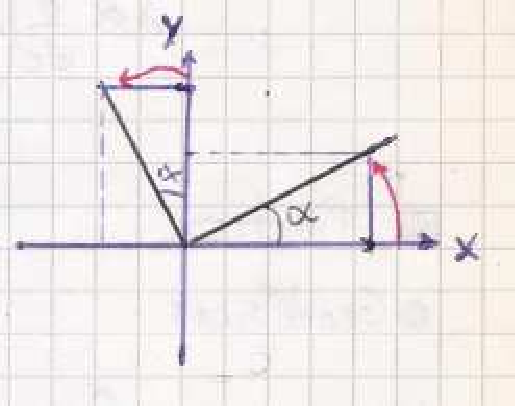
\includegraphics[width=0.35\textwidth]{images/fig_mc_noether1.pdf}	 
	\end{center}
	\caption{}
	\label{fig_mc_noether1}
\end{figure} 

Si consideramos el lagrangiano de una partícula libre en dicho plano $ \Lag = 1/2 m (\dot{x}^2 + \dot{y}^2)$, la 
cantidad conservada será 
\[
	m \dot{x} \delta x + m \dot{y} \delta y = 2\epsilon ( -p_x y + p_y x ) = cte.
\]
que no es otra cosa que el momento angular $L_z$ (que se conserva).

Por supuesto, para una rotación general (no restringida a un plano) son necesarios tres parámetros.
La rotación plana requiere solamente un parámetro.
\end{ejemplo}

% ~~~~~~~~~~~~~~~~~~~~~~~~~~~~~~~~~~~~~~~~~~~~~~~~~~~~~~~~~~~~~~~~~~~~~~

En el caso de una partícula rebotando en un billar hay simetría de rotación en torno a $z$, luego hay
constante de movimiento. En el caso del movimiento elíptico donde 1 y 2 son los focos no hay simetría
de rotación pero aún así hay constante de movimiento $ \ell_1 \ell_2 $.

\begin{figure}[!htb]
	\begin{center}
	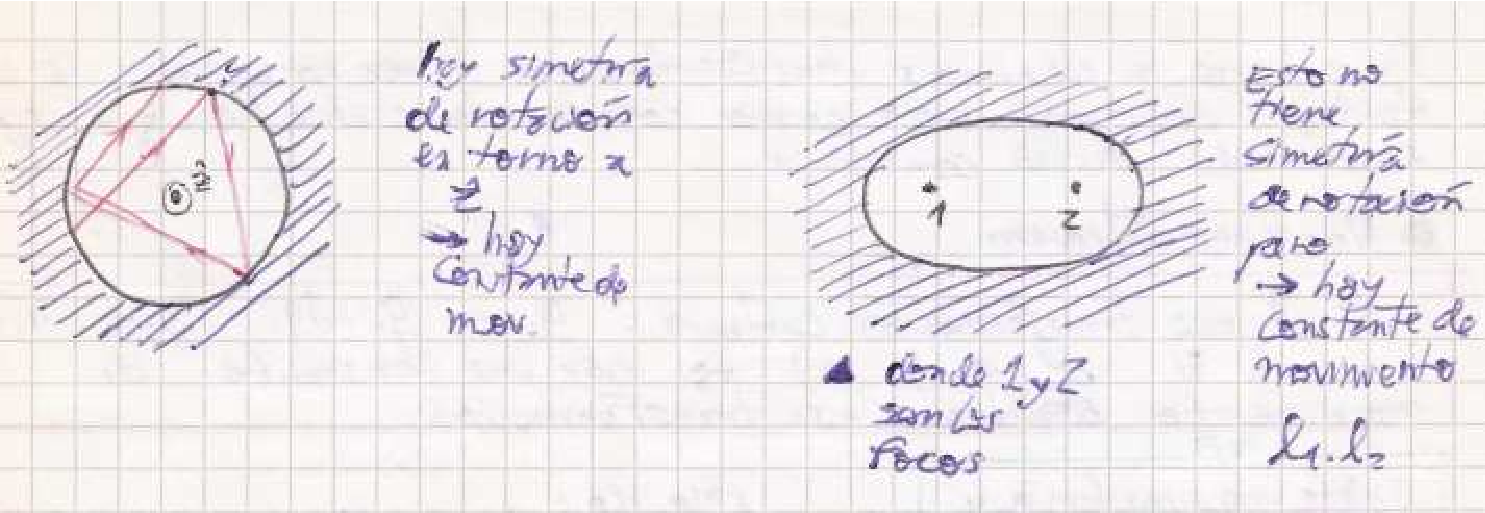
\includegraphics[width=1.0\textwidth]{images/fig_mc_noether2.pdf}	 
	\end{center}
	\caption{}
	\label{fig_mc_noether2}
\end{figure} 

\subsection{Rotación infinitesimal}

\notamargen{En la carpeta estaba este tema. Aparentemente para una rotación general aparecía el momento angular 
conservado, si se manipulaban adecuadamente los índices.}

Recordemos que 
\[
	\delta q_i = q'_i - q_i 
\]
y una traslación infinitesimal es 
\[
	\vb{r}_i' - \vb{r}_i = \delta \vb{r}. 
\]

La variable cíclica es un caso particular de teorema de Noether, pero hay constantes de movimiento que 
no provienen de ninguna simetría.
\[
	\frac{d}{dt}\left( \sum_i \dpar{\Lag}{\dot{q}_i} ( \delta \alpha \hat{n}\times \vb{r}_i ) \right) 
\]
\[
	\frac{d}{dt}\left( \delta\alpha \sum_i \vb{p}_i \times \vb{r}_i  \right) =
	\delta\alpha \frac{d}{dt}\left(  \sum_i \vb{p}_i \times \vb{r}_i  \right) = 0
\]
siendo $\delta \alpha \equiv \epsilon$ un parámetro infinitesimal.
Para $k$ grados de libertad
\begin{align*}
	q'_i &= q_i + \underbrace{\epsilon_i g_i(q_1,...,q_n,t)}_{\delta q} \\
	... \\
	q'_k &= ...
\end{align*}
\[
	\vb{r}_i' = \vb{r}_i + \delta\vb{r} \quad \textrm{traslación rígida}
\]
\[
	\vb{r}_i' = \vb{r}_i + \delta\alpha \; \hat{n}\times\vb{r}_i \quad \textrm{rotación rígida}
\]
o también 
\[
	\delta \vb{r} \times \vb{r}
\]

$T$ es invariante siempre frente a (por ser un escalar)
\[
	T = T' 
\]
entonces habrá que examinarlo.
Constatemos que 
\[
	V = V(|\vb{r}_i - \vb{r}_j|)
\]
es invariancia ante una traslación rígida, y
\[
	V = V(x_1,x_2)
\]
es una invariancia de traslación en $x_3$.

$\Lag$ tendrá como constante un momento lineal si $V$ es invariante frente a traslación.
$\Lag$ tendrá como constante un momento angular si $V$ es invariante frente a rotación.
$\Lag$ tendrá como constante una combinación si $V$ es invariante frente a una roto-traslación.

Otra construcción posible es 
\[
	\delta \Lag = 0
\]
\[
	\Lag( q_i , \dot{q}_i, t ) - \Lag(q_i' , \dot{q}_i' , t) = 0 
\]
pidiendo que $d\Lag = 0$ llego a 
\[
	\sum \left\{ \frac{d}{dt}\left( \dpar{\Lag}{\dot{q}_i} \delta q \right) - 
	\frac{d}{dt}\left( \dpar{\Lag}{\dot{q'}_i} \delta q' \right)  \right\} = 0
\]
\notamargen{Las primas están mal. Hay que pensar una construcción adecuada.
Queda odd.}
\[
	\sum \left\{ \frac{d}{dt}\left( \dpar{\Lag}{\dot{q}_i} \delta q \right) - 
	\frac{d}{dt}\left( \dpar{\Lag}{\dot{q'}_i} \delta q \right) -
	\frac{d}{dt}\left( \dpar{\Lag}{\dot{q'}_i} \sum_\ell^s \epsilon_\ell g_i^\ell \right) \right\} = 0
\]
y podemos usar que 
\[
	\dpar{\Lag}{\dot{q'}_i} = \dpar{\Lag}{\dot{q}_i}
\]
pues $g\neq g(t)$ y es todo a tiempo fijo. Se tiene 
\[
	q' = q + \delta q
\]
\[
	q_i' = q_i + \sum_\ell^s \epsilon_\ell g_i^\ell
\]
siendo esta la transformación general
\[
	\delta q_i' = \delta q_i + \sum_\ell^s \epsilon_\ell g_i^\ell
\]

Extraemos también que 
\[
	\dpar{\Lag}{\dot{q'}_i} \sum_\ell^s \epsilon_\ell g_i^\ell = C
\]

Se puede pensar también como que $\Lag$ es invariante ante la transformación infinitesimal
$\delta q$
\[
	\delta\Lag = 0 = \sum_i^N \dpar{\Lag}{q_i}\delta q_i + \dpar{\Lag}{\dot{q}_i}\delta \dot{q}_i
\]
\[
	\delta\Lag = 0 = \sum_i^N \left[ \dpar{\Lag}{q_i} - \frac{d}{dt}\left( \dpar{\Lag}{\dot{q}_i} \right)
	\right]\delta q_i  + \sum_i^N \frac{d}{dt}\left( \dpar{\Lag}{\dot{q}_i} \delta q_i \right)  = 0
\]
siendo el primer término nulo, y siendo lo que se conserva lo que aparece en el segundo término,
donde 
\[
	\delta q_i =  \sum_\ell^s \epsilon_\ell g_i^\ell(q_1,q_2,...,q_n)
\]
Finalmente 
\[
	\delta \Lag = 0 = \frac{d}{dt}\left( \sum_i^N \dpar{\Lag}{\dot{q}_i} \delta q_i \right) 
\]


% =================================================================================================


% \bibliographystyle{CBFT-apa-good}	% (uses file "apa-good.bst")
% \bibliography{CBFT.Referencias} % La base de datos bibliográfica

\end{document}

	
		\documentclass[10pt,oneside]{CBFT_book}
	% Algunos paquetes
	\usepackage{amssymb}
	\usepackage{amsmath}
	\usepackage{graphicx}
	\usepackage{libertine}
% 	\usepackage[bold-style=TeX]{unicode-math}
	\usepackage{lipsum}

	\usepackage{natbib}
	\setcitestyle{square}

	\usepackage{polyglossia}
	\setdefaultlanguage{spanish}


	\usepackage{CBFT.estilo} % Cargo la hoja de estilo
	
	% Tipografías
	% \setromanfont[Mapping=tex-text]{Linux Libertine O}
	% \setsansfont[Mapping=tex-text]{DejaVu Sans}
	% \setmonofont[Mapping=tex-text]{DejaVu Sans Mono}

	%===================================================================
	%	DOCUMENTO PROPIAMENTE DICHO
	%===================================================================

% \title{CBFT Mecánica clásica}
% \author{Fuerzas centrales}
% \date{\today}

\begin{document}
% \maketitle
% \tableofcontents

\chapter{Fuerzas centrales}

% =================================================================================================
\section{Fuerzas centrales}\index{Fuerzas centrales}
% =================================================================================================

\notamargen{Comentario de que fijo un punto, y es una función vectorial tomar vector y da vector, que resulta finalmente
más simple porque se sabe de antemano la dirección de la salida --en la dirección de la recta que une los puntos--.}

Una fuerza central es aquella que depende únicamente de la distancia entre dos puntos. Es decir que si se tienen dos
puntos $\vb{x}, \vb{y}$, separados una distancia $ r = |\vb{r}| = |\vb{x} - \vb{y}| $, una fuerza central $\vb{F}$ verifica
\[
	\vb{F}( \vb{x}, \vb{y} ) = F(r) \: \hat{r}, \qquad \qquad \hat{r} = \frac{\vb{r}}{r}
\]
% es decir que la fuerza $\vb{F}$ entre dos puntos $\vb{x}, \vb{y}$ depende de la distancia $r = |\vb{x}-\vb{y}|$
% entre los mismos.
de manera que la información sobre la dirección de la misma ($\hat{r}$) está establecida en la recta que une $\vb{x}$ con 
$\vb{y}$ mientras que su módulo es una función escalar $F(r)$.


\begin{figure}[!hbt]
	\begin{center}
	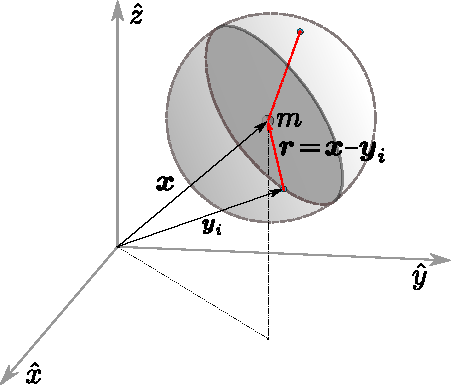
\includegraphics[width=0.4\textwidth]{images/fig_fuerza_central.pdf}	 
	\end{center}
	\caption{}
\end{figure} 

Esto implica, al ser una fuerza dependiente de una sola coordenada, que siempre es posible obtener un potencial
a partir de ella, es decir que existe $V(r)$ tal que
\[
	F(r) = - \dpar{V}{r}.
\]
\notamargen{Hay que elaborar bastante aquí: la fuerza central implica la simetría esférica porque tomado como origen
de coordenadas uno de los dos puntos $\vb{x}$ o $\vb{y}$, la fuerza por otro punto que se halle a la misma distancia
$r$ tendrá la misma magnitud. Además, el torque de la fuerza respecto a ese origen será nulo puesto que son paralelos
$\vb{r}$ y $\vb{F}$. Anoté en la carpeta: el lagrangiano es un potencial de superficies equipotenciales esféricas, entonces
se conserva el momento angular.}

Entonces, para una partícula libre el lagrangiano se puede escribir en coordenadas esféricas $(r,\theta,\phi)$ como
\[
	\Lag = \frac{1}{2}m \left( \dot{r}^2 + r^2 \dot{\theta}^2 + r^2 \sin(\theta)^2\dot{\phi}^2 \right)
\]

El momento angular $\vb{L}$ se conserva puesto que $\vb{\tau} = \vb{x} \times \vb{F}=0$. Como es 
$\vb{L} = \vb{x} \times \vb{p} = \vb{x} \times m \: \dot{\vb{x}} = cte$ entonces se sigue que $\vb{r},\vb{p}$
se hallan contenidos en el mismo plano.

Puedo pedir, sin pérdida de generalidad, que $\theta=\pi/2$ (se sitúa la partícula en el plano $xy$) y entonces
se tienen dos grados de libertad,
\[
	\Lag = \frac{1}{2}m \left( \dot{r}^2 + r^2 \dot{\theta}^2 \right) - V(r).
\]

Como $\phi$ es cíclica se tiene
\be
	\dpar{\Lag}{\dot{\phi}} = L = mr^2\dot{\phi}
	\label{ec_mov_uno}
\ee
que no es otra cosa que la conservación del momento angular (la primera ecuación de movimiento). Esa información puede 
ser llevada al lagrangiano,
\be
	\Lag = \frac{1}{2}m \dot{r}^2 + \left[ \frac{L^2}{2 m r^2} - V(r) \right]
	\label{lag_pot_central}
\ee
donde el último corchete será lo que llamaremos un potencial efectivo\footnote{Debido a la conservación del momento 
angular la parte de la energía dependiente de $\phi$, o mejor dicho debida a la rotación en $\phi$ se ha podido 
expresar en términos de $r$; entonces pasa a formar parte del potencial.}\index{potencial efectivo} $V_{\text{eff}}$, y 
el lagrangiano adopta la forma
\[
	\Lag = \frac{1}{2}m \dot{r}^2 + V_{\text{eff}}(r).
\]
Digamos que el potencial efectivo sería todos aquellos términos que no tienen la forma de la energía cinética 
(cuadrática en velocidades).
Notemos que ahora el lagrangiano depende solamente de $r$; el problema ha resulado para un único grado de libertad.

Dado el sistema elegido (movimiento plano en $xy$) ahora el $p_\phi$ es el $L$ total; en cambio, de haber elegido otro 
plano el $p_\phi$ sería el $L_z$.

La ecuación de Euler-Lagrange para el lagrangiano \eqref{lag_pot_central} resulta en
\[
	m\ddot{r} - \frac{L^2}{mr^3} + \dpar{V}{r} = 0.
\]
Integrando esta ecuación se llega a la conservación de la energía pero podemos utilizar el hecho de saber que la 
misma se conserva y escribir su expresión explícita
\be
	E = T - V = \frac{1}{2}m \dot{r}^2 + \frac{L^2}{2 m r^2} + V(r).
	\label{ec_mov_dos}
\ee

A partir de estas constantes $L,E$ tengo dos ecuaciones de primer orden \eqref{ec_mov_uno} y \eqref{ec_mov_dos}. Se han 
podido {\it ahorrar} dos integraciones: la integral de $\ddot{r}$ para obtener $\dot{r}$ y la integral de $\ddot{\phi}$ 
para hallar $\dot{\phi}$.

Desde la ecuación \eqref{ec_mov_dos} se puede integrar directamente la trayectoria $r=r(t)$ según
\[
	\dtot{r}{t} = \sqrt{ \frac{2}{m}\left( E - \frac{L^2}{2 m r^2} - V(r) \right)},
\]
o bien 
\[
	\int_{t_i}^{t_f} dt = \int_{r(t_i)}^{r(t_f)} \frac{dr}{\sqrt{\frac 2 m ( E - \frac{L^2}{2 m r^2} - V(r) )}},
\]
integral que en principio siempre tiene solución.
A partir de la ecuación \eqref{ec_mov_uno} se puede obtener la trayectoria en el espacio físico $r=r(\phi)$, o 
equivalentemente $\phi=\phi(r)$.
\[
	\dtot{\phi}{t} = \dtot{\phi}{r} \dot{r} =  \frac{L}{mr^2} 
\]
e incorporando de la \eqref{ec_mov_dos} la expresión de $\dot{r}$ se puede llegar a 
\[
	\int_{\phi_i}^{\phi_f} d\phi = \int_{r(\phi_i)}^{r(\phi_f)} 
	\frac{L}{\sqrt{ 2 m r^4 \left( E - \frac{L^2}{2 m r^2} - V(r) \right)}}dr
\]
y la resolución total del problema dependerá de la forma $V(r)$.

En el gráfico bajo estas líneas ilustramos muchas de las características de la física del problema
de fuerzas centrales.

\notamargen{Embellecer un poco las expresiones por el aspecto odd de las raíces y todo eso.}

\begin{figure}[hbt]
	\begin{center}
	\includegraphics[width=0.9\textwidth]{images/fig_mc_potencialcentral.pdf}	 
	\end{center}
	\caption{}
\end{figure} 

% =================================================================================================
\section{Solución a partir de las ecuaciones de Euler-Lagrange}
% =================================================================================================

\[
	m \ddot{r} -\frac{L^2}{m r^3} -\dpar{V}{r}= 0 
\]
\[
	d \phi = \frac{L}{m r^2} dt \qquad \longrightarrow \quad  \dpar{\phi}{r}\dpar{r}{t}  = \frac{L}{m r^2}
\]
\[
	\frac{d}{t}(\dot{r}) = \frac{L}{m r^2} \frac{d}{\phi}(\dot{r})
\]
\[
	m \dtot[2]{r}{t} -\frac{L^2}{m r^3} = -\dpar{V}{r}
\]
\[
	\frac{L}{r^2} \frac{d}{\phi}\left( \dtot{r}{t} \right) -\frac{L^2}{m r^3} = -\dtot{V}{r}
\]
\[
	\frac{L}{r^2} \frac{d}{\phi}\left( \frac{L}{m r^2}\dtot{r}{\phi} \right) -\frac{L^2}{m r^3} = -\dtot{V}{r}
\]
y acá probamos el conveniente cambio de variables
\[
	U = \frac{1}{r} \qquad dU = -\frac{1}{r^2} dr 
	\qquad \dtot{U}{\phi} = -\frac{1}{r^2}\dtot{r}{\phi} = -U^2\dtot{r}{\phi}
\]
\[
	U^2 L \frac{d}{d\phi} \left\{ -\frac{L}{m}\dtot{U}{\phi} \right\} - \frac{L^2}{m r^3} U^3 = F(1/U)
\]
\[
	- \frac{U^2 L^2}{m} \dtot[2]{U}{\phi} - \frac{L^2}{m r^3} U^3 = F(1/U)
\]
\[
	- \frac{U^2 L^2}{m} \left[ \dtot[2]{U}{\phi} + U \right] = F(1/U)
\]
o bien
\[
	\left[ \dtot[2]{U}{\phi} + U \right] = - \frac{F(1/U) m}{U^2 L^2}. 
\]

En el caso del potencial de Kepler será 
\[
	\left[ \dtot[2]{U}{\phi} + U \right] = - \frac{K m}{L^2},
\]
es decir que el miembro derecho es una constante. Sale fácil entonces.

% =================================================================================================
\section{Velocidad areolar}\index{Velocidad areolar--}
% =================================================================================================

\[
	\dot{\phi} = \frac{L}{m r^2}
\]
\begin{figure}[hbt]
	\begin{center}
	\includegraphics[width=0.4\textwidth]{images/fig_mc_velareolar.pdf}	 
	\end{center}
	\caption{}
\end{figure} 
De la figura puede verse que 
\[
	A = \frac{1}{2} r^2 d\phi 
\]
y  entonces
\[
	\dtot{A}{t} = \frac{1}{2} r^2 \dtot{\phi}{t} = \frac{1}{2} r^2 \dot{\phi} = \frac{1}{2}\frac{L}{m} = cte.
\]

% =================================================================================================
\section{Las fuerzas centrales y las leyes de Kepler}
% =================================================================================================

Tenemos 
\[
	\int d\phi = \int \frac{(L/Mr^2)}{\sqrt{ \frac{2}{m}(E - V_{\text{eff}})}} dr	\qquad
	\dtot[2]{U}{\phi} + U  = - \frac{F(1/U) m}{U^2 L^2} \quad U = 1/r
\]
que es simétrica respecto a $\phi$ y $-\phi$. Esto determina una simetría orbital si
tomamos
\[
	U(\phi=0) = U_0 	\qquad		\left. \dtot{U}{\phi} \right|_{\phi=0}= 0
\]
lo cual significa que $U_0$ es un extremo (punto apsidal).

Calculemos ahora el ángulo que recorre una oscilación completa,
\[
	\Delta \phi = 2\int_{r_m}^{r_M} \frac{(L/Mr^2)}{\sqrt{ \frac{2}{m}(E - V_{\text{eff}})}} dr
\]

Si $\Delta \phi = 2 q $ siendo $q= (m/n)\pi $ son $m,n \in \mathbb{Z}$ entonces
\[
	\Delta \phi = 2 \frac{m}{n} \pi 
\]
\[
	\frac{m}{n} = \frac{2\pi}{\Delta \phi}
\]
y esto significaría que la órbita se cierra.

La ecuación a resolver es 
\[
	\dtot[2]{U}{\phi} + \left( U  - \frac{k m}{L^2} \right) = 0.
\]
Si consideramos una nueva variable 
\[
	\beta = U  - \frac{k m}{L^2}
\]
la anterior pasa a 
\[
	\dtot[2]{\beta}{\phi} + \beta = 0
\]
y es fácil ver que la solución es
\[
	\beta = A \cos( \phi -\phi_0 ),
\]
o bien 
\be
	U(\phi) = \frac{km}{L^2} +  A \cos( \phi -\phi_0 ),
	\label{sol_general}
\ee
donde $A,\phi_0$ son constantes. Ahora bien, la expresión \eqref{sol_general} es la solución general,
necesitamos proveer las condiciones iniciales para fijar $ A, \phi_0 $. Propongamos $ \phi_0 = 0 $
punto apsidal.
\notamargen{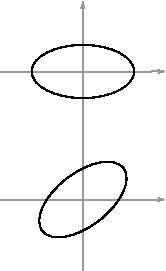
\includegraphics[width=0.3\textwidth]{images/fig_mc_detalle_elipses.pdf}
Eligiendo el punto $\phi_0 =0$ obtenemos una elipse como la de arriba.
}
Luego podemos utilizar $r_m, r_M$ lo cual determina $U_m, U_M$ respectivamente, cuyos valores son 
\[
	U^M_m = \frac{km}{L^2} \left( 1 \pm \sqrt{1 + \frac{2EL^2}{k^2 m} }\right)
\]

y esto nos permite fijar $A$. Incorporando esto en \eqref{sol_general} y recordando que $U(\phi) =1/r$ 
se tiene 
\[
	\frac{1}{r} = \frac{km}{L^2}\left( 1 +  \sqrt{1 + \frac{2EL^2}{k^2 m} } \cos( \phi ) \right),
\]
que no es otra cosa que la ecuación de una elipse en coordenadas polares con origen en un foco.
Veámoslo.

% \[
% 	\frac{1}{r} = \frac{km}{L^2} +  A \cos( \phi -\phi_0 )
% \]
% y habría que usar $r_m, r_M$ para evaluar $A$.

Las elipses verifican 
\[
	\frac{x^2}{a^2} + \frac{y^2}{b^2} = 1	\qquad \sigma^2 = a^2 - b^2
\]
donde $\sigma$ es la semi-distancia focal. Definiendo $ \sigma/a \equiv \varepsilon$ (la excentricidad) 
se puede expresar
\[
	b = a \sqrt{ 1 - \varepsilon^2 }
\]
\notamargen{Falta el sistema de coordenadas en el foco $f'$. Revisar quién es $EL$.}
\begin{figure}[hbt]
	\begin{center}
	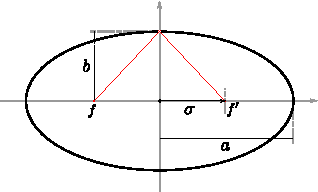
\includegraphics[width=0.4\textwidth]{images/fig_mc_elipse_1.pdf} \hspace*{2em}	 
	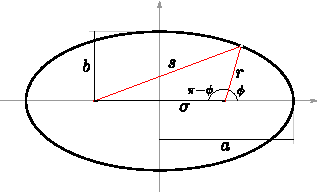
\includegraphics[width=0.4\textwidth]{images/fig_mc_elipse.pdf}	 
	\end{center}
	\caption{}
	\label{fig_mc_elipse}
\end{figure} 

Por otro lado, usando el teorema del coseno para el triángulo definido en la Figura \ref{fig_mc_elipse} es 
\[
	s^2 = (2\sigma)^2 + r^2 - 4\sigma r \cos( \pi - \phi )
\]
y como $s+r$ es la distancia que se mantiene constante e igual, entre otras, a $2a$ se sigue que 
\[
	( 2a -r )^2 = 4\sigma^2 + r^2 + 4\sigma r \cos(\phi)
\]
cuya simplificación conduce a
\[
	\frac{1}{r} = \frac{1 + \varepsilon \cos (\phi)}{a(1-\varepsilon)} = \frac{a}{\phantom{^a}b^2} \left( 1 + 
\varepsilon \cos (\phi) \right)
\]
la cual es la ecuación de una elipse.

\notamargen{Acá hay que hacer un laburo muy importante.}
% \begin{figure}[hbt]
% 	\begin{center}
% 	\includegraphics[width=0.4\textwidth]{images/fig_mc_elipse.pdf}	 
% 	\end{center}
% 	\caption{}
% \end{figure} 

Entonces en resumen, las leyes de Kepler son
\begin{enumerate}
 \item Los planetas giran en órbitas elípticas con el Sol en uno de sus focos. Esto es común de los potenciales del 
tipo 
	\[
		V \propto 1/r
	\]
 \item El radio vector recorre áreas iguales en tiempos iguales
	\[
		\delta A = \frac{1}{2} r^2 \delta \phi \quad \longrightarrow \quad \dtot{A}{t} = \frac{r^2}{2} 
\dot{\phi} = \frac{L}{2m} (cte.)
	\]
	Esto es una característica de todo potencial central.
 \item El cubo del semieje mayor de la órbita de un planeta es proporcional al cuadrado del período empleado en 
recorrerla.
	La ecuación anterior, que da la velocidad areolar, se puede integrar como 
	\[
		\int dA  = \frac{L}{2m} \int dt
	\]
	que conduce a 
	\[
		\pi a b = \frac{L}{2m} \tau \qquad \longrightarrow \qquad a = \frac{L\tau}{2\pi b m}, 
	\]
	y luego, como $k m /L ^2 = a/b^2$ llegamos a 
	\[
		a^3 = \frac{k}{m} \frac{1}{4\pi^2} \: \tau^2 = \frac{GM}{4\pi^2} \tau^2
	\]
 y esto es independiente de la masa del planeta.
 
Como $a$ depende de $L$ se tiene que dependiendo de la energía $E$ tendré órbitas como las ilustradas debajo
todas las cuales tienen la misma energía 
\[
	a = \frac{1}{2}(r_M + r_m) = -\frac{k}{2E}
\] 
\notamargen{Esto estaba en la carpeta pero no lo entiendo bien del todo. Tal vez ilustración de la elipse con 
el sistema coordenado en el origen.}
 Para una elipse con el sistema coordenado en el centro se tiene 
 \[
	\frac{1}{r^2} = \frac{1}{b^2}( 1-\varepsilon^2 \cos^2 (\phi) )
 \]
 
 Trabajamos más con la elipse,
 \[
	r_M + r_m = 2a
 \]
 \[
	E = \frac{L^2}{2mr^2} - \frac{k}{r}	\qquad\qquad E - \frac{L^2}{2m} U^2 - kU = 0
 \]
 \[
	\frac{1}{r_{m,M}} = \frac{ \frac{2mkE}{L^2} \mp \sqrt{ \left(\frac{2mkE}{L^2}\right)^2 + \frac{8mE}{L^2} } }{2}
 \]
 \[
	\frac{1}{r_{m,M}} = \frac{mEk}{L^2} \left( 1 \pm \sqrt{1 - \frac{2L^2}{mEk^2}}\right) 
 \]
 y acá constatamos que representa una elipse; es decir que las órbitas son elípticas.
\end{enumerate}

\begin{ejemplo}{\bf Problema 1 de central forces}

Conviene pasarlo a un problema equivalente para una partícula {\it masa reducida} en términos del centro de masa.
\[
	E = \frac M 2 V_{cm}^2 + \frac \mu 2 ( \dot{r}^2 + r^2\dot{\theta}^2 ) + V( r )
\]
\[
	\tau = \frac{2\pi R}{R\dot{\theta}}
\]

\includegraphics[scale=0.4]{images/fig_mc_central_forces1.jpg}

\[
	E = \frac 1 2 \mu(\dot{r}^2 + r^2\dot{\theta}^2 ) + \frac K r
\]
Al detenerlas,
\[
	E = - \frac K r
\]
y al rearrancar
\[
	E = \frac 1 2 \mu \dot{r}^2 - \frac K r
\]
\includegraphics[scale=0.4]{images/fig_mc_central_forces2.jpg}

Para la integración le pongo el signo negativo puesto que corresponde a la situación física correcta
\[
	\dtot{r}{\tau} = -\sqrt{ \frac 2 \mu \left(E + \frac K r \right) }
\]
Integración a ambos miembros lleva a
\[
	\int_0^\tau dt = - \int_R^0 \frac{dr}{ \sqrt{ \frac 2 \mu \left(E + \frac K r \right) } }
\]
o bien a 
\[
	\tau' = \sqrt{\frac{\mu}{2}} \sqrt{\frac{R}{K}} \int_R^0 \sqrt{\frac{r}{R-r}} dr
\]

Con el cambio de variables $U=\sqrt{R-r}$ que lleva al diferencial 
\[
	dU = \frac{-dr}{2\sqrt{R-r}}
\]
la integral resulta en 
\[
  	2 \left( \frac{ \mu R }{ 2K } \right) \int_0^{\sqrt{R}} \sqrt{ R - U^2 } dU =
 	2 \left( \frac{\mu R}{2K}\right) \left( \frac{ U\sqrt{R-U^2} }{2} + \frac{R}{2} 
 	\asen\left( \frac{U}{\sqrt{R}}\right) \right)
\]
que se ha buscado en tablas.
Luego,
\[
	\tau' = \sqrt{ \frac{\mu R}{2K} }\frac{R\pi}{2}
\]
y las ecuaciones de Newton,
\[
	\frac{K}{R^2} = \mu R\dot{\theta}^2 
\]
de la cual se puede despejar $\dot{\theta}$ para obtener
\[
	\tau = 2 \pi R \sqrt{\frac{\mu R}{K}}
\]
de manera que 
\[
	\frac{ \tau }{ \tau' } = 4 \sqrt{ 2 }.
\]
\end{ejemplo}

\begin{ejemplo}{\bf Problema 4 de central forces}

Consideramos un potencial de la forma 
\[
	V(r) = \frac{K}{r^2}
\]
que es un potencial repulsivo puesto que 
\[
	F(r) = -\dpar{V}{r} = \frac{2K}{r^3}
\]
implica que {\it aleja a la partícula}.
Como es central, conserva $ L = m r^2 \dot{\theta} $ se puede escribir la energía como
\[
	E = \frac 1 2 m ( \dot{r}^2 + r^2 \dot{\theta}^2 ) + \frac K {r^2} = \frac{ m \dot{r}^2 }{2} +
	\left( \frac{ \ell }{ 2 m r^2 } + \frac{ K }{ r^2 } \right)
\]

\includegraphics[scale=0.3]{images/fig_mc_potencial_central_4.jpg}

Luego,
\[
	\dot{r} = \sqrt{ \frac{2E}{m} - \frac{2L}{2m^2r^2} - \frac{2K}{mr^2} }
\]
y entonces
\[
	m r^2 \sqrt{ \frac{2E}{m} - \frac{2L}{2m^2r^2} - \frac{2K}{mr^2} } \dtot{\theta}{r} = L
\]
de manera que 
\[
	\int_0^{\theta} d\theta = \frac{L}{\sqrt{2m}} \int_{r_0}^{r} \frac{dr}{r^2( E - L/(2mr^2) - K/r^2 )^{1/2}}
\]

Con el cambio de variables $ U = 1 / r $
\[
	\theta = -\frac{L}{\sqrt{2m}} \int_{1/r_0}^{1/r} \frac{ dU }{ [ E - U^2( L/(2m) + K )]^{1/2} }
\]

Integrada da
\[
	\theta = \frac{L}{m\sqrt{2Km + \frac{L^2}{m^2}}}
	\left( \acos\left[ \frac{ \sqrt{2Km + L^2/(m^2)} }{r_0\sqrt{2E/m}} \right] - 
	\acos\left[ \frac{\sqrt{2Km + L^2/(m^2)}}{r\sqrt{2E/m}}\right] \right).
\]

Tomo $r_0$ punto de retorno
\[
	E = \left( \frac{L^2}{2mr_0^2} + \frac{K}{r_0^2} \right)
\]
y entonces
\[
	r_0 = \sqrt{ \frac L {2mE} + \frac K E }
\]
\[
	\theta = \frac{L}{m\sqrt{2Km + \frac{L^2}{m^2}}} \acos\left(\frac{r_0}{r}\right)
\]
y se puede despejar
\[
	r = \frac{r_0}{\cos( \theta m/L \sqrt{ 2Km + L^2/m^2 } )}
\]
\includegraphics[scale=0.3]{images/fig_mc_potencial_central_4_orbitas.jpg}

\end{ejemplo}

% =================================================================================================
\section{Vector de Runge-Lenz}
% =================================================================================================

Para el problema de Kepler también se conserva una cantidad llamada {\it vector de Runge-Lenz} definido como
\[
	\vb{R} = \vb{v} \times \vb{l} - \alpha \frac{\vb{x}}{x}.
\]

Luego, si le tomamos la derivada temporal, resulta
\[
	\dtot{\vb{R}}{t} = \left( \dtot{\vb{v}}{t} \times \vb{l} \right) + \left( \vb{v} \times \dtot{\vb{l}}{t} \right)
	- \alpha\frac{ \vb{v} }{x} + \frac{ \alpha }{x^2} \dtot{x}{t} \vb{x}
\]
donde el último se puede poner en términos de la velocidad si utilizamos la regla de la cadena así
\[
	\dtot{|\vb{x}|}{t} = \dtot{|\vb{x}|}{x_i} \dtot{x_i}{t} = \nabla( |\vb{x}| )\cdot \vb{v} \qquad  \qquad i=1,2,3
\]

Luego, cada componente $i$-ésimo del gradiente de la norma del vector de posición tiene (en coordenadas cartesianas) la 
misma
forma; tomando como ejemplo el $i=1$
\[
	\dtot{|\vb{x}|}{x_1} = \dtot{\sqrt{x_1^2 + x_2^2 + x_3^2}}{x_1} = \frac{x_1}{|\vb{x}|},
\]
de manera que 
\[
	\nabla( |\vb{x}| ) = \frac{\vb{x}}{x} = \hat{x},
\]
el gradiente de la norma del vector es su dirección. Entonces, volviendo a la ecuación original resulta 
\[
	\dtot{\vb{R}}{t} = \left( \dtot{\vb{v}}{t} \times \vb{l} \right) + \left( \vb{v} \times \dtot{\vb{l}}{t} \right)
	- \alpha\frac{ \vb{v} }{x} + \alpha \:\vb{x} \left( \frac{ \pe{x}{v} }{x^3}\right) 
\]

Dado que $\vb{l} = \vb{x} \times m \vb{v}$ el segundo término en la anterior expresión desaparece y nos queda
\[
	\dtot{\vb{R}}{t} = \left( \dtot{\vb{v}}{t} \times [ \vb{x} \times m\vb{v} ] \right) 
	- \alpha\frac{ \vb{v} }{x} + \alpha \:\vb{x} \left( \frac{ \pe{x}{v} }{x^3}\right) 
\]

\notamargen{Aparentemente esto tiene que dar nulo pero no lo estaría viendo.}

\[
	\dtot{\vb{V}}{t} \times ( \vb{x} \times m\vb{v} ) +
	\vb{V} \times \left( \dtot{\vb{r}}{t} \times m\vb{v} + \vb{r} \times m\dtot{\vb{v}}{t} \right)
\]
pero como $\dtot{\vb{r}}{t} \times m\vb{v} = 0$ resulta lo que resulta.
\begin{figure}[hbt]
	\begin{center}
	\includegraphics[width=0.4\textwidth]{images/fig_mc_rungelenz.pdf}	 
	\end{center}
	\caption{}
\end{figure} 

El vector de Runge-Lenz siempre apunta en la misma dirección dada su constancia (ver figura).
\notamargen{Mejorar la figura!}

Escribo $ T = E - V $
\[
	r_{max} m v^2 = 2Er_{max} + 2\alpha
\]
pero 
\[
	r_{max} = \frac{2 E l^2 \alpha}{\alpha^2 m (1-\varepsilon)} = \frac{-1}{\alpha}\frac{b^2 
\alpha}{\alpha^2(1-\varepsilon)}
\]
\[
	r_{max} = - (1+\varepsilon) \alpha
\]

\[
	b^2 = a^2( 1 - \varepsilon^2 )
\]

\begin{ejemplo}{\bfseries Vector de Runge-Lenz en órbitas elípticas}
\notamargen{Este título es provisorio}

Sabemos que el vector de Runge-Lenz tiene la forma 
\[
	\vb{A} = \pv{V}{L} - \alpha \frac{\vb{x}}{x}
\]
y cumple 
\[
	\dtot{A}{t} = 0
\]

Veamos qué expresión tiene el módulo $ A \equiv |\vb{A}| $. Tomando el producto escalar 
\[
	\pe{A}{x} = A r \cos \theta = ( \pv{V}{L} )\cdot \vb{x} - \alpha \frac{\pe{x}{x}}{x}
\]
y reescribiendo (ciclicidad del producto vectorial)
\[
	( \pv{V}{L} )\cdot \vb{x} = \vb{L} \cdot ( \pv{r}{v} ) = \vb{L} \cdot \frac{ \vb{L} }{m} = \frac{L^2}{m}
\]
y entonces
\[
	\alpha r \left( 1 + \frac{A}{\alpha} \cos \theta \right) = \frac{L^2}{m}
\]
pero como $ (1 + \varepsilon \cos \theta ) = p / r $ es la excentricidad se tiene $ A = \varepsilon \alpha $.

\end{ejemplo}

% =================================================================================================
\section{Orbitas de potenciales centrales}
% =================================================================================================

\[
	V(r) = -\frac{\alpha}{r}
\]
\[
	V(r) = \frac{ k r^2 }{2}
\]
Estos dos casos dan órbitas cerradas. Pero hay otros potenciales interesantes.
El potencial de Yukawa
\[
	V(r) = - \frac{\euler^{-\lambda r}}{r^\alpha}
\]
que es aproximadamente como un potencial coulombiano apantallado ($\alpha=1,\lambda=0$).
Otro es el oscilador no armónico\index{Oscilador no armónico}
\[
	V(r) = r^\alpha
\]
Algunos casos se muestran bajo estas líneas

\begin{figure}[hbt]
	\begin{center}
	\includegraphics[width=0.6\textwidth]{images/fig_mc_potenciales_otro.pdf}
	\end{center}
	\caption{Algunas curvas de potenciales anarmónicos $ r^\alpha $.}
\end{figure}

Da órbita que no se cierra en un billar elíptico.

\begin{figure}[hbt]
	\begin{center}
	\includegraphics[width=0.4\textwidth]{images/fig_mc_billar.pdf}
	\end{center}
	\caption{.}
\end{figure}

% =================================================================================================
\section{Reducción del problema de dos cuerpos a uno equivalente}
% =================================================================================================

Para dos partículas de masas $ m_1 $ y $ m_2 $ sometidas a una fuerza central 
\[
	\vb{F}_{21} = F(r) \hat{r}_{21} \qquad \qquad F(r) = -\dtot{V(r)}{r}
\]
siendo $x \equiv |\vb{x}_2-\vb{x}_1|$ la distancia relativa.

\begin{figure}[hbt]
	\begin{center}
	\includegraphics[width=0.4\textwidth]{images/fig_mc_prob_equiv_scheme.pdf}	 
	\end{center}
	\caption{.}
	\label{fig_mc_prob_equiv_scheme}
\end{figure} 

La energía del sistema será de la forma  $ E = T_1 + T_2 + V(r) $ pero se puede expresar según 
$ E = T_{cm} + T_{rel} + V(r) $; es decir separando la energía cinética en el aporte del centro de
masa más un aporte que depende de la distancia relativa entre los cuerpos.
De modo idéntido para el momento angular podemos pasar de $ L_{total} = L_{cm} + L_{spin} $ donde el
momento angular de spin es el referido al movimiento en torno al centro de masas.

\notamargen{Revisar y consolidar toda la notación aquí, que está mezclada.}
Consideramos el siguiente sistema de coordenadas,
\[
	r \equiv | \vb{r}_2 - \vb{r}_1 | \qquad	\qquad  \dot{r} \equiv | \dot{\vb{r}}_2 - \dot{\vb{r}}_1 |
\]
donde el sistema centro de masas es
\[
	\vb{R}_{cm} = \frac{ m_1\vb{r}_1 + m_2\vb{r}_2 }{ m_1 + m_2 }	\qquad 
	M \vb{V}_{cm} =  m_1\vb{v}_1 + m_2\vb{v}_2 
\]
\[
	0 = m_1\vb{r}_1' + m_2\vb{r}_2'
\]
que provocan
\[
	\vb{r}_1' = -\frac{m_2}{m_1}\vb{r}_2' \qquad   \vb{r}_2' = -\frac{m_1}{m_2}\vb{r}_1' 
\]
dando unas $r$ relativas
\be
	\vb{r} = \vb{r}_1' - \vb{r}_2' = -\frac{ m_1 + m_2 }{ m_1 } \vb{r}_2' = -\frac{ m_1 + m_2 }{ m_2 } \vb{r}_1'.
	\label{r_relativas}
\ee

\begin{figure}[hbt]
	\begin{center}
	\includegraphics[width=0.4\textwidth]{images/fig_reduccion.pdf}	 
	\end{center}
	\caption{Sistema coordenado para la reducción del problema de dos cuperpos al de uno equivalente.}
\end{figure} 

Luego, como la energía se conserva (el $V_{cm}=cte.$) podemos escribir
\[
	E = \frac{1}{2} m_1 \dot{\vb{r}}_1^2 + \frac{1}{2} m_2 \dot{\vb{r}}_2^2 + V(r)
\]
\[
	E = \frac{1}{2} m_1 ( \dot{\vb{R}} + \dot{\vb{r}}_1' )^2 + \frac{1}{2} m_2 ( \dot{\vb{R}} + \dot{\vb{r}}_2' )^2 
+ V(r)
\]
\[
	E = \frac{1}{2} m_1 ( {\vb{V}} )^2 +  \frac{1}{2} m_1 ( \dot{\vb{r}}_1' )^2 + 
		\frac{1}{2} m_2 ( {\vb{V}})^2 + \frac{1}{2} m_2 (\dot{\vb{r}}_2' )^2 + V(r)
\]
\[
	E = \frac{1}{2} M {\vb{V}}^2 + \frac{1}{2} \frac{m_2^2}{m_1} \dot{\vb{r}}_2'^2 + \frac{1}{2} m_2 
\dot{\vb{r}}_2'^2 + V(r)
\]
\[
	E = \frac{1}{2} M {\vb{V}}^2 + \frac{1}{2} \frac{m_2 m_1}{M} \dot{\vb{r}}^2 + V(r).
\]

Pero como $E$ y la $\vb{V}$ se conservan, se tiene 
\[
	e \equiv E - \frac{1}{2} M {\vb{V}}^2 =  \frac{1}{2} \mu \dot{\vb{x}}^2 + V(r)
\]
donde $e$ es una cantidad conservada que podemos llamar la energía reducida[?].

Este último $\vb{x}$ es un vector distancia relativa. Es un problema equivalente para la partícula
centro de masas.

\begin{figure}[hbt]
	\begin{center}
	\includegraphics[width=0.4\textwidth]{images/fig_mc_prob_equiv.pdf}	 
	\end{center}
	\caption{.}
	\label{fig_mc_prob_equiv}
\end{figure} 

Podemos considerar ahora los momentos angulares de las partículas respecto de este sistema centro
de masas. Así
\[
	\vb{l}_1' = \vb{x}_1' \times \vb{p}_1 \qquad \qquad  \vb{l}_2' = \vb{x}_2' \times \vb{p}_2'
\]
y sus módulos verifican 
\[
	|\vb{l}_1'| = {x}^{2'}_1 m_1 \dot{\theta} \qquad \qquad  |\vb{l}_2'| = {x}^{2'}_2 m_2 \dot{\theta}
\]
de manera que 
\be
	\ell = ( {x}^{2'}_1 m_1 + {x}^{2'}_2 m_2 ) \dot{\theta} = \mu r^2 \dot{\theta}
	\label{mom_ang_conserv}
\ee
es el momento angular de spín para este sistema. Nótese que a partir de \eqref{r_relativas} se puede
expresar las $x'_i$ ($i=1,2$) en términos de $r$.

Luego, en coordenadas polares en el centro de masa resulta
\[
	e = \frac{1}{2} \mu ( \dot{ r}^2 + r^2\dot{\phi}^2 ) + V(r),
\]
o bien, usando \eqref{mom_ang_conserv},
\[
	e = \frac{1}{2} \mu \dot{ r}^2 + \frac{\ell^2}{2 \mu r^2 } + V(r)
\]
que no es otra cosa que el problema de fuerza central para un cuerpo de masa $\mu$.

Diremos que la {\it distancia relativa} describe una elipse. Las trayectoria reales en el espacio físico
son dos elipses confocales. Por supuesto dejan de cumplirse las leyes de Kepler en este caso.

Si como solución proponemos
\[
	V(r) = -\frac{\alpha}{r}
\]
tendré $ r = r(\phi) $ una elipse, que es lo que describe el $ r $ relativo.
Se descompondrá el movimiento según las ecuaciones de transformación
\[
	\vb{r}_1'= -\frac{m_2}{m_1+m_2} \vb{r} \qquad \text{ Elipse de dirección contraria a $\vb{r}$}
\]
\[
	\vb{r}_2'= \frac{m_1}{m_1+m_2} \vb{r} \qquad \text{ Elipse de dirección igual a $\vb{r}$}	
\]
Tendremos dos elipses confocales como muestra la figura bajo estas líneas 

\begin{figure}[hbt]
	\begin{center}
	\includegraphics[width=0.4\textwidth]{images/fig_mc_elipses_confocales.pdf}	 
	\end{center}
	\caption{.}
	\label{fig_mc_elipses_confocales}
\end{figure} 

En este caso ya dejan de cumplirse las leyes de Kepler
\[
	\dtot{\mathcal{A}}{t} = \frac{\ell}{2\mu} \qquad a^3 \sim \tau^2 
\]
para la órbita relativa.
\[
	\frac{\pi a b }{\tau}= \frac{\ell}{2\mu} 
\]
\[
	b = \frac{\ell}{\sqrt{\alpha \mu}} a^{1/2} \qquad \frac{a}{b} = \frac{\mu \alpha}{\ell^2}
\]
\[
	\frac{\pi a^{3/2}}{\sqrt{\alpha \mu} \tau} = \frac{1}{2\mu}
\]
y entonces ahora se ve que no es independiente de las masas y no se puede simplificar $\sqrt{\mu\alpha}$ con
$\mu$ como ocurría en un movimiento elíptico tradicional (bajo potencial gravitatorio).
Entonces no es válida la ley de Kepler.
% =================================================================================================
\section{Dispersión}
% =================================================================================================

Consideramos la dispersión de un haz de partículas de cierta energía cinética por un centro dispersor,
ver ilustración.

\begin{figure}[htb]
	\begin{center}
	\includegraphics[width=0.5\textwidth]{images/fig_mc_dispersion1.pdf}	 
	\end{center}
	\caption{}
\end{figure} 
\[
	d\sigma = \frac{dN}{n}
\]
donde $dN$ es el número de partículas dispersadas entre $\chi$ y $\chi + d\chi$ y $n$ es el número de
partículas emitidas por tiempo y por área. De esta forma $d\sigma$ tiene unidades de área.

Consideramos $d$ centro dispersor con simetría esférica (cilíndrica basta).
Usamos como suposiciones que todo lo que emerge entre $\rho + d\rho$ - $\rho$  es dispersado entre
$\chi + d\chi$ - $\chi$, y que se conservan tanto $E$ como \vb{L}.

\begin{figure}[htb]
	\begin{center}
	\includegraphics[width=0.5\textwidth]{images/fig_mc_dispersion2.pdf}	 
	\end{center}
	\caption{}
\end{figure}

El anillo se dispersa en un sector esférico. Entonces podemos establecer las siguientes conclusiones
para el anillo entre $\rho + d\rho$ - $\rho$, a saber
\[
	A =  \pi ( (\rho + d\rho)^2 - \rho^2 ) \qquad \longrightarrow A \approx 2 \pi \rho \: d\rho,
\]
entonces
\[
	d\sigma = \frac{  2 \pi \rho \: d\rho I}{I}
\]
donde $\rho$ es el parámetro de impacto y $I$ el número de partículas por unidad de tiempo y área.
Finalmente
\[
	d\sigma =  2 \pi \rho(\chi) \left| \dtot{\rho}{\chi} \right| d\chi
\]

Como se conservan la energía y el momento angular
\[
	E = \frac{1}{2} m V_\infty^2 \qquad L = m \rho V_\infty^2 
\]
\begin{figure}[htb]
	\begin{center}
	\includegraphics[width=0.5\textwidth]{images/fig_mc_dispersion3.pdf}	 
	\end{center}
	\caption{}
\end{figure}
En general se desconoce $V(r)$.

Se puede calcular el ángulo $\varphi_0$ de acuerdo a 
\[
	\chi = \pi - 2\varphi_0,
\]
donde
\[
	\varphi_0 = \int_{r_m}^{\infty} \frac{L/mr^2}{\sqrt{\frac{2}{m}(E - V_{\text{eff}})}} dr
\]
\[
	\chi = \pi - 2 \varphi_0 (\rho)
\]
e invertimos desde la última ecuación.

Veamos el caso de una esfera maciza. En general los cuerpos duros equivalen a un potencial del tipo
\[
	V = \begin{cases}
	     \infty \qquad \textrm{cuerpo}\\
	     \;0 \qquad \; \textrm{fuera} \\
	    \end{cases}
\]
\begin{figure}[htb]
	\begin{center}
	\includegraphics[width=0.5\textwidth]{images/fig_mc_dispersion4.pdf}	 
	\end{center}
	\caption{}
\end{figure}
\[
	\chi = \pi - 2\varphi_0
\]
\[
	\sin(\varphi_0) = \frac{\rho}{a} \qquad d\rho = -a \frac{1}{2}\cos \left(\frac{\pi-\chi}{2}\right)
\]
y entonces 
\[
	d\sigma = 2\pi a^2 \sin\left(\frac{\pi-\chi}{2}\right) \frac{1}{2}\cos\left(\frac{\pi-\chi}{2}\right) d\chi
\]
\[
	d\sigma = \frac{\pi}{2} a^2 \sin( \pi-\chi) d\chi = \frac{\pi}{2} a^2 \sin( \chi) d\chi
\]
y como hay que integrar $\chi$ de 0 a $\pi$
\[
	\int_0^\pi \frac{\pi}{2} a^2 \sin( \chi) d\chi = \pi a^2
\]
\[
	\sigma = \pi a^2
\]
En el caso de los cuerpos duros la sección eficaz es la sombra de los mismos.
\notamargen{Sobre el ángulo sólido
\[
\Omega = \textrm{Area}/r^2
\]
\[
d\Omega = 2 \pi \sin( \chi ) d\chi 
\]
\[
\Omega = 4 \pi 
\]
para la esfera.
}


% =================================================================================================
\section{Dispersión por dos cuerpos}
% =================================================================================================

Consideramos el caso de un cuerpo que se fracciona en dos (creo?)
\begin{figure}[htb]
	\begin{center}
	\includegraphics[width=0.5\textwidth]{images/fig_mc_disp2body1.pdf}	 
	\end{center}
	\caption{}
\end{figure} 
Desde el centro de masa
\[
	\vb{P}_1 + \vb{P}_2 = 0
\]
\[
	m_1 \vb{v}_1 + m_2 \vb{v}_2 = 0
\]
definimos una velocidad relativa
\[
	\vb{v} \equiv \vb{v}_2  - \vb{v}_1 = \vb{v}_2 \left( \frac{ m_1 + m_2 }{ m_1 }\right) .
\]
\begin{figure}[htb]
	\begin{center}
	\includegraphics[width=0.5\textwidth]{images/fig_mc_disp2body2.pdf}	 
	\end{center}
	\caption{}
\end{figure} 
Con respecto a la energía,
\[
	\frac{1}{2} M \vb{V}_{cm}^2 + e_{int} = \frac{1}{2} m_1 \vb{v}_1^2 + \frac{1}{2} m_2 \vb{v}_2^2
						+ e_{int 1 } + e_{int 2} + \frac{1}{2} M \vb{V}_{cm}^2
\]
\[
	\frac{1}{2} m_1 \vb{v}_1^2 + \frac{1}{2} m_2 \vb{v}_2^2 = e_{int} - e_{int 1 } - e_{int 2} = \Delta e
\]
y pasando todo en términos de la velocidad relativa
\[
	 \frac{1}{2} \frac{m1 m2}{ m_1 + m_2 } v = \Delta e
\]
entonces 
\[
	v = \sqrt{\frac{ 2 \Delta e}{ \mu } }.
\]
\begin{figure}[htb]
	\begin{center}
	\includegraphics[width=0.5\textwidth]{images/fig_mc_disp2body3.pdf}	 
	\end{center}
	\caption{}
\end{figure} 

El problema es evidentemente plano.
\[
	\vb{V}_1^L =  \vb{V}_{cm} + \vb{V}_1' \qquad \longrightarrow \quad ( \vb{V}_1^L - \vb{V}_{cm} ) = \vb{V}_1'
\]
\[
	{V_1^L}^2 - V_{cm} - 2 {\vb{V}_1^L}^2 \vb{V}_{cm} = V_1^2
\]
\[
	{V_{1x}^L}^2 + {V_{1y}^L}^2 - V_{cm} - 2 {V_{1x}^L}^2 V_{cm} = V_1^2
\]
\[
	( V_{1x}^L  - V_{cm} )^2 + {V_{1y}^L}^2 = V_1^2
\]
que es una circunferencia.
\[
	\tan(\theta) = \frac{V_1 \sin(\chi) }{ V_{cm} + V_1 \cos(\chi) }
\]
\begin{figure}[htb]
	\begin{center}
	\includegraphics[width=0.45\textwidth]{images/fig_mc_disp2body4a.pdf}	 
	\includegraphics[width=0.45\textwidth]{images/fig_mc_disp2body4b.pdf}
	\end{center}
	\caption{}
\end{figure} 

Esto tiene dos raíces $\chi_{1,2}$ si $ V_{cm} > V_1$. 

Si $ V_{cm} > V_1$ hay una sola $V$ de las partículas.

Si $ V_{cm} < V_1$ hay partículas emitidas hacia atrás vistas desde L.

Si pensamos en una distribución isótropa de partículas, desde el centro de masa
\[
	e = \frac{1}{2} m_1 V_{1}^2
\]
\[
	V_L^2 = V_1^2 + V_{cm}^2 - 2 V_1 V_{cm} \cos( \pi -\chi )
\]
a iguales $V_1,V_{cm}$ se tienen variables $V_L, \chi$, entonces
\[
	dV_L^2 = - 2 V_1 V_{cm} \sin(\chi) d\chi
\]
\[
	\frac{dV_L^2}{2 V_1 V_{cm}} = \sin( \chi) d\chi 
\]
\[
	d\sigma = 2 \pi \rho |\dtot{\rho}{\chi}| d\chi 
\]
\[
	d\Omega = 2 \pi \sin( \chi ) d\chi 
\]
\[
	\frac{d\Omega}{4\pi} = \frac{1}{2} \sin( \chi ) d\chi 
\]
\[
	\frac{d\Omega}{4\pi} =  \frac{d (V_L^2) }{4 V_1 V_{cm}} = \frac{1}{2} \frac{d ( 1/2 m_1 V_L^2) }{m_1 V_1 V_{cm}} 
\]

% =================================================================================================
\section{Scattering}
% =================================================================================================

Tenemos dos suposiciones básicas:
	\begin{itemize}
		\item Interacción elástica.
		\item Conservación de energía y de momento.
	\end{itemize}

\begin{figure}[htb]
	\begin{center}
	\includegraphics[width=0.5\textwidth]{images/fig_mc_scatt1.pdf}	 
	\end{center}
	\caption{}
\end{figure} 	
	
Desde el centro de masa se tienen:
\[
	\vb{P} = \vb{P}_1 + \vb{P}_2 = 0	\qquad		\vb{r} \equiv \vb{r}_2 + \vb{r}_1
	\qquad		\vb{V} \equiv \vb{V}_2 - \vb{V}_1
\]
donde los últimos son las posiciones y velocidades relativas.
\[
	E = \frac{1}{2} M \vb{V}_{cm}^2 + \frac{1}{2} \mu \vb{V}^2 + V(r)
\]
\[
	m_1 \vb{V}_1 + m_2 \vb{V}_2 = 0 \qquad m_1 \vb{V}_1 = -\frac{m_2}{m_1} \vb{V}_2.
\]
\begin{figure}[htb]
	\begin{center}
	\includegraphics[width=0.7\textwidth]{images/fig_mc_scatt2.pdf}	 
	\end{center}
	\caption{}
\end{figure} 
En términos de las velocidades relativas
\[
	\vb{V}_2 = \frac{m_1}{m_1 + m_2} \vb{V} \qquad \vb{V}_1 = -\frac{m_2}{m_1 + m_2} \vb{V}
\]
Se puede escribir la energía cinética del siguiente modo
\[
	T = \frac{1}{2} m_1 \vb{V}_{1-in}^2 + \frac{1}{2} m_2 \vb{V}_{2-in}^2 =
	\frac{1}{2} M \vb{V}_{cm}^2 + \frac{1}{2} m_1 \vb{V}_{1-cm}^2 + \frac{1}{2} m_2 \vb{V}_{2-cm}^2 
\]
\[
	T - \frac{1}{2} M \vb{V}_{cm}^2 \equiv t = \frac{1}{2} \frac{m_1 m_2}{m_1 + m_2} \vb{V}^2 =
							\frac{1}{2} \mu \vb{V}^2
\]

\[
	\vb{V}_1^L = \vb{V}_{cm} - \frac{m_2}{M} \vb{V}	\qquad \vb{V}_2^L = \vb{V}_{cm} - \frac{m_1}{M} \vb{V}
\]

\[
	\vb{p}_1^L = m_1 \vb{V}_{cm} - \mu \vb{V} = m_1 \frac{\vb{P}}{M} - \mu \vb{V}
\]
\[
	\vb{p}_2^L = m_2 \vb{V}_{cm} + \mu \vb{V} = m_2 \frac{\vb{P}}{M} + \mu \vb{V}
\]
\begin{figure}[htb]
	\begin{center}
	\includegraphics[width=0.35\textwidth]{images/fig_mc_scatttriangle.pdf}	 
	\end{center}
	\caption{}
\end{figure} 
Donde 
\[
	\vb{V}_{cm} + \vb{V}_1 = \vb{V}_1^L
\]
\[
	\vb{p}_2^L = \frac{m_2}{M} \vb{P} + \mu \vb{V}\hat{n}		\qquad	 \vb{p}_1^L = \frac{m_1}{M} \vb{P} - \mu \vb{V}\hat{n}
\]
\[
	\frac{m_2}{M} \vb{P} + \frac{m_1}{M} \vb{P} = \vb{P} = \vb{p}_2^L + \vb{p}_1^L
\]
\[
	\tan(\theta_2) = \frac{P_1 \sin(\chi)}{ (m_2/M) P + P_1\cos(\chi)}
\]

% =================================================================================================
\section{Dispersión por potenciales infinitos}
% =================================================================================================

La idea es que sabiendo $\rho$ (parámetro de impacto) quiero saber qué ángulo $\chi$ se desvían las
partículas incidentes.
\begin{figure}[htb]
	\begin{center}
	\includegraphics[width=0.7\textwidth]{images/fig_mc_potinf.pdf}	 
	\end{center}
	\caption{}
\end{figure} 
\[
	\phi_0 + \alpha = \frac{\pi}{2}		\qquad		2 \phi_0 + \alpha + \beta = \pi
	\qquad \phi_0 + \beta = \frac{\pi}{2}
\]
\[
	\alpha = \beta		\qquad 		2\alpha = 2\beta = \chi
\]
\[
	\dtot{\rho}{z} = \tan \left(\beta \right) = \tan\left(\frac{\chi}{2}\right)
\]
\[
	\tan\left(\frac{\chi}{2}\right) = \dtot{\rho}{z} = \frac{ d\rho/dz }{ dz/d\theta }
\]
con $\theta$ variable paramétrica. Donde $\rho = \rho(z)$ es la función que da la curva roja (el perfil
del cuerpo dispersor).



% =================================================================================================

% \bibliographystyle{CBFT-apa-good}	% (uses file "apa-good.bst")
% \bibliography{CBFT.Referencias} % La base de datos bibliográfica

\end{document}

	
		\documentclass[10pt,oneside]{CBFT_book}
	% Algunos paquetes
	\usepackage{amssymb}
	\usepackage{amsmath}
	\usepackage{graphicx}
	\usepackage{libertine}
% 	\usepackage[bold-style=TeX]{unicode-math}
	\usepackage{lipsum}

	\usepackage{natbib}
	\setcitestyle{square}

	\usepackage{polyglossia}
	\setdefaultlanguage{spanish}


	\usepackage{CBFT.estilo} % Cargo la hoja de estilo

	% Tipografías
	% \setromanfont[Mapping=tex-text]{Linux Libertine O}
	% \setsansfont[Mapping=tex-text]{DejaVu Sans}
	% \setmonofont[Mapping=tex-text]{DejaVu Sans Mono}

	%===================================================================
	%	DOCUMENTO PROPIAMENTE DICHO
	%===================================================================

\begin{document}

\chapter{Pequeñas oscilaciones}

Es un formalismo para analizar el movimiento que realiza un sistema cuando está sometido a
ligeras perturbaciones en la posición de equilibrio.
Esto desarrollará un método sistemático para tratar todo tipo de problemas con muchos grados
de libertad pero en forma aproximada.

\subsection{Idea para un grado de libertad}

Para un grado de liberada la idea es que 

\includegraphics[scale=0.5]{images/fig_mc_oscil_1.jpg}

en un potencial $V(x)$ con un mínimo, es decir que cumple 
\[
	\dtot{V(x)}{x} = 0 ,\dtot[2]{V(x)}{x} > 0
\]
para algún $x_{eq}$, en la expresión de la energía
\be
	E = \frac 1 2 m \dot{x}^2 + V(x),
	\label{energia_1d}
\ee
se aproxima el potencial según\footnote{Nótese que esta es la expansión de Taylor en la cual el término lineal 
está justamente ausente porque la derivada primera en el punto es nula.}
\be
	V(x) \approx V_0 + \frac{1}{2} \left.\dtot[2]{V(x)}{x}\right|_{x_{eq}} (x-x_{eq})^2,
	\label{potencial_aproximado}
\ee
y si definimos $ k \equiv d^2V/dx^2|_{x_{eq}} $ se llega a 
\[
	E = \frac 1 2 m \dot{x}^2 + V_0 + \frac{1}{2} k (x-x_{eq})^2, 
\]
que derivada con respecto al tiempo resulta en 
\[
	m\ddot{x} + k (x-x_{eq}) = 0,
\]
la cual no es otra cosa que una ecuación de oscilador armónico, cuya solución general es
\[
	x(t) = A \cos (\omega t + \varphi ),
\]
donde $ \omega =  \sqrt{ k / m } $ y $ \varphi $ está asociada a la energía $E$. Ver Apéndice X para la resolución
de oscilador armónico.
\notamargen{Un apéndice más: oscilador armónico con término no homogéneo (usar 76R carpeta). Acá habría que llegar a despejar quién es
$\varphi$.}

El problema físico tiene dos constantes aunque la resolución presenta cuatro (dos complejos, con parte real e imaginaria).

Nótese que el desarrollo del potencial a orden dos equivale a una fuerza linealizada, merced a que $ m \ddot{x} = - dV/dx$.

\subsection{Varias variables}

En el caso de un potencial $V(\vb{x}_1, ...,\vb{x}_n)$ hay que hallar las raíces del mismo y luego desarrollar en torno a los puntos
de equilibrio. Se empieza desde 
\[
	\dpare{V}{\vb{x}}{x_{eq}} = 0,
\]
y habría que desarrollar 
\[
	V( \vb{x}_1, ...,\vb{x}_n ) = V( \vb{x}_1, ...,\vb{x}_n ) + 
	\frac 1 2 \sum_{i,j} \dparcru{V}{\vb{x}_i}{\vb{x}_j}(\vb{x}-\vb{x}_i)(\vb{x}-\vb{x}_j)
\]

No obstante, el problema se puede enfocar mejor en términos de las coordenadas generalizadas. Entonces, el potencial es
\[
	V(q_1,...,q_n) \approx V(q_1^0,...,q_n^0) + \sum_{i=1}^n \left. \dpar{V}{q_i} \right|_{q_i^0} (q_i - q_i^0)
		+ \frac{1}{2} \sum_{i,j=1}^n \left. \dparcru{V}{q_j}{q_i}\right|_{q_i^0}(q_i -q_i^0)(q_j -q_i^0)
\]
y la energía cinética,
\[
	T(q_1,...,q_n,\dot{q}_1,...,\dot{q}_n) \approx \frac{1}{2} \left( m(q_1^0,...,q_n^0) + \sum_{i=1}^n 
				\left. \dpar{m}{q_i} \right|_{q_i^0} (q_i - q_i^0) + ... \right) \sum_{i,j}^n \dot{q}_i\dot{q}_j
\]
[Esta expresión hay que revisarla y reubicarla!]

La energía cinética es 
\[
	T = \frac 1 2 \sum_{i,j} m_{ij}(q_1,...,q_n) \dot{q}_i \dot{q}_j
\]
donde $m_{ij}$ son los coeficientes de las coordenadas generalizadas y se desarrollarán en serie en torno al equilibrio (caracterizado
por un supraíndice $0$), es decir,
\[
	m_{ij} \approx m_{ij}( q_i^0, ..., q_n^0 ) + \sum_k \dpare{ m_{ij} }{ q_k }{q^0}( q_k - q_k^0 ).
\]

Estamos considerando que la energía cinética es $ T = T_2 $, pero cabría pensar que existe un $ T_0( q_1,...,q_n)$ y se lo 
sumaríamos en ese caso al potencial $V$. En el lagrangiano que consideraremos no está presente $T_1$; queremos un potencial
que no depende de las velocidades.

\begin{ejemplo}{Sobre el término $T_1$}

Para el caso de una masa fija, enhebrada en varilla que gira con velocidad angular $\omega$, el lagrangiano es
\[
	\Lag = \frac 1 2 m (\dot{r}^2 + r^2 \dot{\vp}^2),
\]
con energía
\[
	T = T_0 + T_2 = \frac{2}{2}mr^2\dot{\vp}^2 + \frac{2}{2}m\dot{r}^2
\]
donde $\dot{\vp} = \omega$ el último término no depende de la velocidad pero sí de la posición.
Es {\it como} un potencial que genera la fuerza ficticia.
\end{ejemplo}

\notamargen{Esta aproximación y formalismo sirve para un mínimo y un sistema que hace pequeños apartamientos
respecto de ese mínimo.}

Haciendo la aproximación consistente resulta 
\[
	\Lag = T - V = - \frac{1}{2} \sum_{i,j}^n \left. \dparcru{V}{q_j}{q_i}\right|_{q_i^0}(\eta_i)(\eta_j) +
		\frac{1}{2} \sum_{i,j}^n \left. m_{ij}\right|_{q_i^0} \dot{\eta}_i \dot{\eta}_j
\]
con $V_{ij} \equiv \partial^2 V / ( \partial q_i \partial q_j ) |_{q_i^0}, m_{ij} = m_{ij}|_{q_i^0}$, ambos simétricos, 
y donde se ha definido $\eta_i = q_i - q_i^0$, que es un apartamiento típico de la posición de equilibrio. 
Notemos que $\dot{q}_i = \dot{\eta}_i $. Nótese también que el término lineal en
la aproximación de $m_{ij}$ al verse multiplicado por el producto $\dot{q}_i\dot{q}_j$ es ya de orden cúbico por lo cual debe
descartarse para ser consistentes con las aproximaciones hechas en el potencial.

Con esta nomenclatura puede escribirse el {\it lagrangiano de pequeñas oscilaciones}
\[
	\Lag = \frac{1}{2} \sum_{i,j=1}^n m_{ij} \dot{\eta}_i \dot{\eta}_j - \frac{1}{2} \sum_{i,j=1}^n V_{ij} \eta_i \eta_j
\]
siendo ambas sumatorias formas bilineales cuadráticas reales y definidas positivas. Matricialmente,
\[
	\Lag = \frac{1}{2} \dot{\vb{\eta}}^t \mathbb{T} \dot{\vb{\eta}} - \frac{1}{2} \dot{\vb{\eta}}^t \mathbb{V} \dot{\vb{\eta}}
\]
y si ahora evaluamos las ecuaciones de Euler-Lagrange para este formalismo resulta que 
\[
	\frac{d}{dt}\left( \dpar{\Lag}{\dot{\eta}_k} \right) - \dpar{\Lag}{\eta_k} = 
		\frac{d}{dt} \left( \frac{1}{2} \sum_{i,j=1}^n m_{ij} \frac{d}{d\dot{\eta}_k}(\dot{\eta}_i \dot{\eta}_j) \right) - 
		\frac{1}{2} \sum_{i,j=1}^n V_{ij} \frac{d}{d\eta_k} (\eta_i \eta_j) = 0
\]
son $n$ ecuaciones diferenciales de Euler, 
\[
	\sum_{j=1}^n m_{kj} \ddot{\eta}_j + V_{kj} \eta_j = 0 \qquad k=(1,...,n).
\]

Esto es un oscilador armónico para cada partícula. Se puede pensar en todas las partículas unidas por resortes acoplados.

Se propone como solución 
\[
	\eta_j(t)  = A_j e^{i\omega t}
\]
de frecuencia $\omega$, idéntica para todas las partículas, tomando al final del proceso $\Re\{A_j e^{i\omega t}\}$ como 
solución física. Esta elección lleva a
\[
	\sum_{j=1}^n ( - \omega^2 m_{kj} + V_{kj} ) A_j = 0
\]
que equivale a
\[
	(\mathbb{V} -\omega^2\mathbb{T})\vb{A} = 0
\]
que no es otra cosa que un problema de autovalores y autovectores generalizado. Necesito
\[
	\left| \mathbb{V} -\omega^2\mathbb{T} \right| = 0
\]
lo cual me hará buscar un polinomio característico $P^n[\omega^2]$ de orden $n$ en $\omega^2$.
Así se trendrán $n$ valores para $\omega^2$ con $\omega^2_s \in \mathbb{R}$ y $\omega^2_s \geq 0$, que serán las
autofrecuencias o frecuencias propias $\omega^2_1, ...,\omega^2_n$. 

Para cada $\omega$ se tiene una solución
\[
	\eta_j^s = A_j^s e^{i\omega_s t}	 \qquad s=1,...,N
\]
pero el movimiento general será una combinación de todas las frecuencias,
\[
	\eta_j(t) = \sum_{s=1}^N c_s A_j^s e^{i\omega_s t}.
\]

En general, dado un $V=V(q_i)$ puede ser más fácil obtener explícitamente la serie de Taylor con 
$\partial^2 V/ \partial q_i \partial q_j |_{q_i^0}$ o bien cambiar variable $\eta = q_i - q_i^0$ y quedarse
con los términos cuadráticos en $\eta_i \eta_j$. Para la energía cinética $T=T(q,\dot{q})$ puede ser más
fácil evaluar $m_{ij}(q_i)|_{q_i^0}$ y quedarnos con los términos cuadráticos en $\dot{\eta}_i \dot{\eta}_j$.

Veamos la solución para una frecuencia dada,
\[
	\sum_j ( V_{kj} - \omega_s^2 m_{kj} ) A_j^s = 0
\]
y como usamos una raíz $\omega_s$ se tendrá una ecuación linealmente dependiente que tiraremos. Serán
ahora $N-1$ ecuaciones,
\[
	\sum_j ( V_{kj} - \omega_s^2 m_{kj} ) \frac{A_j^s}{A_1^s} = 0
\]
y definimos el cociente $a_j^s \equiv {A_j^s}/{A_1^s}$ al pasar dividiendo la amplitud del modo cuya frecuencia estamos
considerando. Entonces
\[
	\sum_j ( V_{kj} - \omega_s^2 m_{kj} ) a_j^s = - V_{k1} - \omega_s^2 m_{k1} \qquad k=1,...,N-1
\]
\notamargen{Acá sería bueno poner explícitamente hasta donde llega la sumatoria y explicitar qué $\omega$ se usa.}

Entonces como $N-1$ ecuaciones no homogéneas tienen solución real, entonces $a_j$ es un cociente real y todo los
$A_s^j$ tienen que tener la misma fase. [mmm?]
La fase viene determinada por las condiciones iniciales.

Veamos ahora que las frecuencias son reales. Para ello se multiplica por el complejo conjugado y se suma
\[
	\sum_k A_k^{s*} \sum_j V_{kj} A_j^s = \omega_s^2 \sum_k A_k^{s*} \sum_j m_{kj} A_j^s
\]
\[
	\sum_k A_k^{s} \sum_j V_{kj} A_j^{s*} = \omega_s^{2*} \sum_k A_k^{s} \sum_j m_{kj} A_j^{s*}
\]
y usando la simetría de $m_{kj}, V_{kj}$ se restan estas ecuaciones y se obtiene
\[
	0 = ( \omega^2_s - \omega^{2*}_s ) \sum_k \sum_j  A_k^{s*} m_{kj} A_j^{s}
\]
y como la doble sumatoria es no nula se sigue que las frecuencias son reales.
Incluso se puede despejar
\[
	\omega_s^2 = \frac{ \sum_k \sum_j  A_k^{s*} V_{kj} A_j^{s} }{ \sum_k \sum_j  A_k^{s*} m_{kj} A_j^{s} }
\]
Ambos, numerador y denominador son definidos positivos.
Si el numerador fuese negativo para alguna dirección, eso significa que en esa dirección será un máximo (sería una
especie de punto silla); pequeñas oscilaciones no valdrá en esa dirección.

Por otra parte, si se consideran dos frecuencias diferentes
\[
	0 = ( \omega^2_s - \omega^{2*}_p ) \sum_k \sum_j  A_k^{s*} m_{kj} A_j^{p}
\]
entonces lo que debe ser nulo es la doble sumatoria. Entonces, en la {\it métrica} dada por $m_{jk}$ $A_j$ y $A_k$
son perpendiculares.
Para determinar el $A_1$ (que era el parámetro que permanecía indeterminado) impongo
\[
	{A^t}^{p*} M A^p = 1
\]
y los $A_j$ se {\it consideran} reales pués todos tienen la misma fase y son los modos normales.
Se está pidiendo que de uno la norma en la métrica dada por $M$.

Si la raíz del polinomio $P^n$ tiene multiplicidad $k$, se tienen $k$ ecuaciones linealmente dependientes y hay que
arrojar al cesto de la basura $k$ ecuaciones.

Si construyo la matriz
\[
	A = \begin{pmatrix}
	A_1^1 & A_1^2 & ... \\
	A_2^1 &       &      \\
	...
	\end{pmatrix},
\]
donde cada columna de esta matriz es un autovector. Entonces se ve que esta matriz {\it diagonaliza} a $M$, i.e.
\[
	A^t M A = \begin{pmatrix}
	1 & 0 & ... \\
	0 &  1  &      \\
	...
	\end{pmatrix} = \mathbb{1}.
\]

Asimismo, como 
\[
	V A = \omega^2 M A,
\]
eso conduce a que 
\[
	A^t V A = \begin{pmatrix}
	\omega_1^2 & 0 & ... \\
	0 &  \omega_2^2  &      \\
	...
	\end{pmatrix}.
\]
\notamargen{Hay que repasar esto.}

\begin{ejemplo}{\bf Lo de las matrices}

Si $ A^{p*} M A^s =0 $ con $ p \neq s $ entonces $M$ está definiendo una métrica pués si $ M = \mathbb{1} $ entonces
\[
	A^{p*} \mathbb{1} A^s = A^{p*} A^s = 0,
\]
lo cual significa que $A^{p*}$ y $ A^s$ son perpendiculares.
 
\end{ejemplo}

\subsection{Expresión vectorial}

Vectorialmente es 
\[
	\vb{\eta}^s = \vb{A}_j^s e^{i\omega_s t} = \begin{pmatrix}
	                A_1 e^{i\omega_s t} \\
	                A_2 e^{i\omega_s t} \\
	                ... \\
	                A_N e^{i\omega_s t} \\
	               \end{pmatrix}
\]
para la frecuencia $\omega_s$, siendo cada uno un grado de libertad moviéndose con frecuencia $\omega_s$.

Luego, es
\[
	\vb{\eta}_{tot} = c_1 \vb{\eta}^1 + c_2 \vb{\eta}^2 + ... + c_N \vb{\eta}^N
\]
\[
	\vb{\eta}_{tot} = \begin{pmatrix}
				\eta_1 \\
				\eta_2 \\
				... \\
				\eta_n 
	                  \end{pmatrix}
	                 = \begin{pmatrix}
				c_1 A_1^1 e^{i\omega t} + c_2 A_1^2 e^{i\omega t} + ... + c_n A_1^n e^{i\omega t} \\
				c_1 A_2^1 e^{i\omega t} + c_2 A_2^2 e^{i\omega t} + ... + c_n A_2^n e^{i\omega t} \\
				... \\
				c_1 A_n^1 e^{i\omega t} + c_2 A_n^2 e^{i\omega t} + ... + c_n A_n^n e^{i\omega t}
	                  \end{pmatrix}
\]
entonces $\vb{A}^s$ es un modo normal de frecuencia $s$.
\[
	\vb{A}^s = \begin{pmatrix}
	            A_1^s \\
	            A_2^s \\
	            ... \\
	            A_n^s
	           \end{pmatrix}
	           e^{i\theta_0}
\]

La solución total ($j$ es el grado de libertad) se puede escribir 
\[
	\eta_j(t) = \sum_{s=1}^N c_s A_j^s e^{i\omega_s t}
\]
\[
	\vb{\eta}(t) = \sum_{s=1}^N c_s \vb{A}^s e^{i\omega_s t}
\]
y finalmente 
\[
	\vb{\eta}(t) = \Re \left\{ \sum_{s=1}^N c_s \vb{A}^s e^{i\omega_s t} \right\}
\]

Matricialmente,
\[
	\vb{A}^\dagger \mathbb{T} \vb{A} = 1
\]
siendo el $\dagger$ el traspuesto conjugado. Se pide que la norma (en la métrica dada por $\mathbb{T}$ de la unidad)
\[
	A^t \mathbb{T} A = \mathbb{1}
\]
lo cual significa que $A$ diagonaliza a $\mathbb{T}$, siendo 
\[
	A = \begin{pmatrix}
	     A_1^1 & A_1^2 & ... & A_1^n \\
	     A_2^1 & ... \\
	     A_n^1 & A_n^2 & ... & A_n^n 
	    \end{pmatrix}
\]
la matriz modal donde sus columnas son autovectores.

\[
	(\mathbb{V} - \omega^2 \mathbb{T})\vb{A} = 0
\]
interpolando a la matriz 
\[
	A^t \mathbb{V} A = \omega^2 A^t \mathbb{T} A= \omega^2 \mathbb{1}
\]

\subsection{Un cambio de coordenadas}

Se puede incluso realizar un cambio de coordenadas
\[
	\vb{\eta} = A \vb{\xi}
\]
tal que 
\[
	A^{n\times n} \xi^{n\times 1} \qquad \qquad  (A \vb{\xi} )^t = {\xi^t}^{1 \times n} {A^t}^{n \times n}
\]
y que se llaman coordenadas normales. Se resuelve el problema en estas coordenadas $\xi$ y luego se regresa a las
originales $\eta$
\[
	\Lag = \frac{1}{2} \dot{\vb{\eta}}^t \mathbb{T} \dot{\vb{\eta}} - \frac{1}{2} \dot{\vb{\eta}}^t \mathbb{V} \dot{\vb{\eta}}
\]
\[
	\Lag = \frac{1}{2} A^t\dot{\vb{\xi}}^t \mathbb{T} A \dot{\vb{\xi}} - \frac{1}{2} A^t\dot{\vb{\xi}}^t \mathbb{V} 
\dot{\vb{\xi}}
\]
\[
	\Lag = \frac{1}{2} \dot{\vb{\xi}}^t \mathbb{1} \dot{\vb{\xi}} - \frac{1}{2} \dot{\vb{\xi}}^t \omega^2 \mathbb{1} \dot{\vb{\xi}}
\]

\[
	\Lag = \frac{1}{2} \sum_i \dot{\vb{\xi}}_i^2 - \frac{1}{2} \sum_i \vb{\xi}_i^2 \omega^2_i 
\]

Los autovectores son los modos normales. Son $N$ osciladores armónicos independientes. Se pasa de un problema de muchas partículas
interactuantes a uno de $N$ partículas que no interactúan.

\[
	\frac{d}{dt}\left( \dpar{\Lag}{\dot{\xi}_i} \right)- \dpar{\Lag}{\xi_i} = \sum_i \ddot{\xi}_i + \omega^2_i \xi_i = 0 
\]
y son $N$ ecuaciones de Euler-Lagrange.
\[
	\sum_i ( -\omega^2 + \omega^2_i ) A_i = 0
\]
de modo que si $\omega^2 = \omega^2_i$ entonces
\[
	\xi_i = C_i e^{i\omega_i t}.
\]

\notamargen{Hay que consolidar este material disperso y confuso!}

\[
	\xi_\ell(t) = C_\ell \cos( \omega_\ell t + \vp_\ell )
\]
y entonces
\begin{align*}
	\eta_1(t) &= \sum_{\ell} A_1^\ell C_\ell \cos( \omega_\ell t + \vp_\ell ) \\
	\eta_2(t) &= \sum_{\ell} A_2^\ell C_\ell \cos( \omega_\ell t + \vp_\ell ) \\
	... & \\
	\eta_N(t) &= \sum_{\ell} A_N^\ell C_\ell \cos( \omega_\ell t + \vp_\ell )
\end{align*}
que son soluciones con $\omega_i \neq 0$. Son $\eta$ coordenadas normales y $\xi$ coordenadas colectivas [no es al revés?].

Digamos que en coordenadas normales
\[
	\xi_j = C_j e^{i \omega_j t}
\]
grados de libertad en $\xi$ (un grado de libertad es una $\omega$) y se desacoplan los grados de libertad
en lo que hace a $\omega_s$.
Por otro lado,
\[
	\eta_j = \sum_{s=1}^N c_s A_j^s e^{i \omega_j t}
\]
grados de libertad en $\eta$, un grado de libertad entonces es combinación lineal de todas las $\omega$.

Si $\omega=0$ es 
\[
	\xi_j = At + B 
\]
\[
	\eta_j = \sum_{s=1}^{N-1} c_s A_j^s e^{i \omega_j t} + A_j(Gt + D)
\]
siendo el último término asociado a la $\omega=0$.
Para volver atrás es 
\[
	A^{\dagger} \mathbb{T} A = \mathbb{1}
\]
y entonces 
\[
	A^{\dagger} \mathbb{T} \vb{\eta} = A^{\dagger} \mathbb{T} A \vb{\xi}  
\]
\[
	A^{\dagger} \mathbb{T} \vb{\eta} = \mathbb{1} \xi
\]
coordenadas normales en función de las de desplazamiento.

En conclusión podemos decir varias cosas,
\begin{itemize}
 \item Las frecuencias nulas están asociadas a momentos conservados.
 \item En coordenadas normales cada grado de libertad oscial con una frecuencia única (son $N$
	osciladores independientes)
 \item Las amplitudes cumplen
 \[ \vb{A}^s =
 \begin{pmatrix}
  a_1^s e^{i \phi_s} \\
  a_2^s e^{i \phi_s} \\
  ... \\
  a_n^s e^{i \phi_s}
 \end{pmatrix}
 \]
 donde tienen la misma fase los $A_j^s$ para toda frecuencia $\omega_s$
 \item Los modos normales pueden excitarse por separado (son ortogonales).
 \item Frecuencias iguales generarán modos normales que son físicamente los
 mismos. Son generados por la simetría del problema.
 \[
	\vb{A} = a_1(v_1) + a_2(v_2)
 \]
 si por ejemplo generan dos autovectores de esta forma.
\end{itemize}

\subsection{Coordenadas colectivas y normales}

\includegraphics[scale=0.5]{images/fig_mc_coord_normales_colectivas.jpg}

Las ecuaciones de Newton del sistema son
\[
	m_1 \ddot{x}_1 = k(x_2-x_1-\ell_0) \qquad \qquad m_2 \ddot{x}_2 = -k(x_2-x_1-\ell_0)
\]
que verifican
\[
	m_1 \ddot{x}_1 + m_2 \ddot{x}_2 = 0,
\]
y entonces
\[
	\ddot{x}_2 - \ddot{x}_1 = -k \left( \frac{1}{m_1} + \frac{1}{m_2} \right) ( x_2-x_1-\ell_0 )
\]

Definiendo $x_2-x_1 = x_{rel}$ se pasa de un problema de dos partículas acopaladas $(x_1,x_2)$ a otro de dos partículas
desacopladas; una oscila y la otra se traslada,
\[
	\mu \ddot{x}_{rel} + k (x_{rel} - \ell_0 ) = 0 \qquad \ddot{x}_{cm} = 0
\]
y $x_{rel}, x_{cm}$ son coordenas colectivas, pero no corresponden a un movimiento real de un sistema.
Tendré dos problemas separados que pueden, dado el caso, excitarse por separado.

En el caso de $N$ osciladores, si hay algún $\omega_i=0$ se tendrá
\[
	\Lag = \sum_{i=1}^N \frac{ 1 }{ 2} \dot{\xi}_i
\]
y como $\ddot{\xi}_i = 0 $ entonces $\xi(t) = At + B$ es solución y 
\[
	\eta_N(t) = \sum_\ell A_n C_\ell \cos (\omega_\ell t + \vp_\ell) + \sum_k A_n^k (Bt + D)
\]
donde el primer término es por $\omega_\ell\neq 0$ y el segundo por $\omega_k=0$.

% ~~~~~~~~~~~~~~~~~~~~~~~~~~~~~~~~~~~~~~~~~~~~~~~~~~~~~~~~~~~~~~~~~~~~~~~~~~~~
\begin{ejemplo}{\bf Aro fijo con bolas engarzadas}
 
\includegraphics[scale=0.5]{images/fig_mc_problema_aro_modos_normales_1.jpg}  

El lagrangiano correspondiente a este {\it setup} es 
\[
	\Lag = \frac 1 2 \left[ \dot{\theta}^2_1 + \dot{\theta}^2_2 + \dot{\theta}^2_3 + \dot{\theta}^2_4 \right] m \ell^2 
	- \frac 1 2 k \ell^2 \left[ ( \theta_2 - \theta_1 )^2 + ( \theta_3 - \theta_2 )^2 + ( \theta_4 - \theta_3 )^2 +
	( \theta_1 - \theta_4 )^2 \right]
\]
Este lagrangiano, como está, ya {\it es} de pequeñas oscilaciones. En efecto, $\theta_2^0 = \theta_1^0 $ de modo que 
$\theta_2 - \theta_1 = \eta_2 - \eta_1 = \theta_2 - \theta_2^0 + \theta_1^0 - \theta_1$. 
Luego,
\[
	V = \begin{pmatrix}
		2k\ell^2 & - k\ell^2 & 0 & -k\ell^2 \\
		\\
		-k\ell^2 & 2 k\ell^2 & -k\ell^2 & 0 \\
		\\
		0 & - k\ell^2 & 2k\ell^2 & -k\ell^2 \\
		\\
		-k\ell^2 & 0 & -k\ell^2 & 2k\ell^2 
	    \end{pmatrix}
\]
donde los ceros reflejan la inexistencia de resorte entre dichas partículas. Entonces
\[
	V - \omega^2 M = \begin{pmatrix}
		2k\ell^2 - m \omega^2 \ell^2 & - k\ell^2 & 0 & -k\ell^2 \\
		\\
		-k\ell^2 & 2 k\ell^2 - m \omega^2 \ell^2 & -k\ell^2 & 0 \\
		\\
		0 & - k\ell^2 & 2k\ell^2 - m \omega^2 \ell^2& -k\ell^2 \\
		\\
		-k\ell^2 & 0 & -k\ell^2 & 2k\ell^2 - m \omega^2 \ell^2
	    \end{pmatrix}
\]
 
Ahora hay que calcular el determinante de esta matriz $V - \omega^2 M$, que luego de desarrollar y usar el método que más le
gusta al dilegencioso lector permite arribar a
\[
	P(\omega) = \mathrm{det}(V - \omega^2 M) = 
	m\ell^2\omega(2k\ell^2 - m\ell \omega^2)^2( m\ell\omega^2-4k\ell^2),
\]
cuyas raíces son:
\[
	\omega_1^2 = 2\frac{k}{m} \qquad 
	\omega_2^2 = 2\frac{k}{m} \qquad 
	\omega_3^2 = 0 \qquad 
	\omega_4^2 = 4\frac{k}{m}
\]

En este ejemplo se conserva el momento angular, de manera que hubiese sido razonable obtener una frecuencia nula 
asociada como de hecho apareció en $\omega_3$. Resolvamos ahora ese modo. Será
\[
	2 k \ell^2 A_1^3 - k \ell^2 A_2^3 - k \ell^2 A_4^3 = 0,
\]
\[
	- k \ell^2 A_1^3 + 2 k \ell^2 A_2^3 - k \ell^2 A_3^3 = 0,
\]
\[
,	- k \ell^2 A_2^3 + 2 k \ell^2 A_3^3 - k \ell^2 A_4^3 = 0
\]
y resulta $A_1^3 = A_2^3 = A_3^3 = A_4^3 $.

Entonces
\[
	\vb{A}^3 = a \begin{pmatrix}
	              1 \\
	              1 \\
	              1 \\
	              1 
	             \end{pmatrix} 
\]
donde $ a = 1 / ( 2 \ell \sqrt{m} ) $ y se da 
\[
	\vb{A}^{3\dagger} M \vb{A}^3 = \mathbb{1}
\]
Este es el modo normal de $\omega^2_3=0$, que se ve dibujado bajo estas líneas
 
\includegraphics[scale=0.5]{images/fig_mc_problema_aro_modos_normales_2.jpg} 

Para la frecuencia $\omega_4$ es 
\[
	- 2 k \ell^2 A_1^4 - k \ell^2 A_2^4 - k \ell^2 A_4^4 = 0,
\]
\[
	k \ell^2 A_1^4 - 2 k \ell^2 A_2^4 - k \ell^2 A_3^4 = 0,
\]
\[
,	- k \ell^2 A_2^4 - 2 k \ell^2 A_3^4 - k \ell^2 A_4^4 = 0
\]
de manera que 
\[
	\vb{A}^4 = a \begin{pmatrix}
	              1 \\
	              -1 \\
	              1 \\
	              -1 
	             \end{pmatrix} 
\]
donde $a = 1/( 2 \ell \sqrt{m})$. El dibujo asociado será

\includegraphics[scale=0.5]{images/fig_mc_problema_aro_modos_normales_3.jpg} 

Para las frecuencias {\it mellizas} $\omega_1,\omega_2 $ es 
\[
	- k \ell^2 A_1^1 - k \ell^2 A_3^1 = 0,
\]
\[
	- k \ell^2 A_2^1 - k \ell^2 A_4^1 = 0,
\]
o bien 
\[
	A_1 = A_3 = 0 \qquad A_2 = A_4,
\]
y
\[
	A_2 = A_4 \qquad A_1 = -A_3
\]
y consecuentemente 
\[
	\vb{A}^1 = a \begin{pmatrix}
	              0 \\
	              1 \\
	              0 \\
	              -1 
	             \end{pmatrix} 
	             \qquad \qquad 
	\vb{A}^2 = a \begin{pmatrix}
	              1 \\
	              0 \\
	              -1 \\
	              0 
	             \end{pmatrix} 
\]
con $ a = 1 /(\ell\sqrt{2m})$. Los dibujos siguientes ilustran los movimientos esperados

\includegraphics[scale=0.5]{images/fig_mc_problema_aro_modos_normales_4.jpg} 

Con respecto a lo de aquí arriba son situaciones físicas iguales (si cambio masas no será la misma situación).
La introducción de $M$ y $m$ (ver figurillas siguientes) rompe la degeneración y serán modos normales pero de diferente 
frecuencia.
Pero podría haberse elegido, ver bajo estas líneas,

\includegraphics[scale=0.5]{images/fig_mc_problema_aro_modos_normales_5.jpg} 

Para el caso siguiente 

\includegraphics[scale=0.5]{images/fig_mc_problema_aro_modos_normales_6.jpg} 

esta configuración no conserva el momento angular.

Si tomamos $M=2m$ entonces podemos considerar momento angular nulo y obtengo un modo normal

\includegraphics[scale=0.5]{images/fig_mc_problema_aro_modos_normales_7.jpg} 
 
\[
	\begin{pmatrix}
	 1 & 1 & 1 & 1 
	\end{pmatrix}
	\begin{pmatrix}
	 1 & 0 & 0 & 0 \\
	 0 & 2 & 0 & 0 \\
	 0 & 0 & 1 & 0 \\
	 0 & 0 & 0 & 2
	\end{pmatrix}
	\begin{pmatrix}
	 1 \\
	 -1/2 \\
	 1 \\
	 -1/2
	\end{pmatrix}
\] 

\notamargen{Este ejemplo se continuó en dos clases consecutivas de modo que puede haber algún pise.}

\includegraphics[scale=0.35]{images/fig_mc_problema_aro_modos_normales_8.jpg} 

En resumen 
\[
	\omega_3^2 = 0 \qquad \qquad A^3 = \frac{1}{2\sqrt{m}\ell}
						\begin{pmatrix} 1 \\ 1 \\ 1 \\ 1 \end{pmatrix}
\]
\[
	\omega_4^2 = \frac{4k}{m} \qquad \qquad A^4 = \frac{1}{2\sqrt{m}\ell}
						\begin{pmatrix} 1 \\ -1 \\ 1 \\ -1 \end{pmatrix}
\]
\[
	\omega_1^2 = \omega_2^2 = \frac{2k}{m}
\]
\[
	A^1 = \frac{1}{\sqrt{2m}\ell}
		\begin{pmatrix} 0 \\ 1 \\ 0 \\ -1 \end{pmatrix}
	A^2 = \frac{1}{2\sqrt{2m}\ell}
		\begin{pmatrix} 1 \\ 0 \\ -1 \\ 0 \end{pmatrix}
\]
\[
	A^t M A = 1
\]

El problema dependerá de cómo excitemos al sistema. Si $\eta = A \xi $ entonces con $\omega_i \neq 0$ es
\[
	\xi_i = C_i \cos (\omega_i t + \vp_i),
\]
pero con $\omega_i = 0$ se tendrá
\[
	\xi_i = B_i t + D_i.
\]

Luego, como $\dot{\eta} = A \dot{\xi} $ de tal modo que 
\[
	A^t M \eta = A^t M A \xi \qquad \qquad  A^t M \dot{\eta} = A^t M A \dot{\xi} = \mathbb{1} \dot{xi}
\]

Las condiciones iniciales serán 
\[
	\eta_1(t=0) = \theta_0 \qquad \eta_i(t=0) = 0, i \neq 1 
\]
y los $\dot{\eta}_i(t=0)$ están en función de las $\eta$ y quiero pasarlas a $\xi$.

\[
	A^t M = \begin{pmatrix}
	        0 & \frac{1}{\sqrt{2m}\ell} & 0 & -\frac{1}{\sqrt{2m}\ell} \\
	        \frac{1}{\sqrt{2m}\ell} & 0 & -\frac{1}{\sqrt{2m}\ell} & 0 \\
	        \frac{1}{2\sqrt{m}\ell} & \frac{1}{2\sqrt{m}\ell} & \frac{1}{2\sqrt{m}\ell} & \frac{1}{2\sqrt{m}\ell} \\
	        \frac{1}{2\sqrt{m}\ell} & -\frac{1}{2\sqrt{m}\ell} & \frac{1}{2\sqrt{m}\ell} & -\frac{1}{2\sqrt{m}\ell} 
	        \end{pmatrix}
	        \begin{pmatrix}
	         m & 0 & 0 & 0 \\
	         0 & m & 0 & 0 \\
	         0 & 0 & m & 0 \\
	         0 & 0 & 0 & m 
	        \end{pmatrix}
\]
mientras que las posiciones iniciales serán 
\[
	\begin{pmatrix}
	0 \\
	\\
	\frac{\sqrt{m}}{\sqrt{2}\ell} \theta_0 \\
	\\
	\frac{\sqrt{m}}{\sqrt{2}\ell} \theta_0 \\
	\\
	\frac{\sqrt{m}}{\sqrt{2}\ell} \theta_0
	\end{pmatrix} =
	\begin{pmatrix}
	\\
	C_1 \cos\vp_1 \\
	\\
	C_2 \cos\vp_2 \\
	\\
	Bt + D \\
	\\
	C_4 \cos\psi_4 \\
	\\
	\end{pmatrix}
\]
y las velocidades iniciales por su parte,
\begin{align*}
	0 & = - C_1 \omega_1 \sin \vp_1 \\
	0 & = - C_2 \omega_2 \sin \vp_2 \\
	0 & = B \\
	0 & = - C_3 \omega_4 \sin \vp_4 
\end{align*}
[tal vez un typo acá arriba]

Al separar de las posiciones de equilibrio se excitan modos que no son el cero, y tendrán momento angular nulo; el
único modo que dará momento angular no nula y por ende generará rotación es el asociado a $\omega_3^2$.

Según se ve el modo uno tampoco se está excitando,
\[
	\vp_2 = 0 \qquad C_2 = \frac{\sqrt{m}}{2\ell} \theta_0
\]
\[
	\eta = A \xi = \begin{pmatrix}
	        0 & \frac{1}{\sqrt{2m}\ell} & \frac{1}{2\sqrt{m}\ell} & \frac{1}{2\sqrt{m}\ell} \\
	        \\
	        \frac{1}{\sqrt{2m}\ell} & 0 & \frac{1}{2\sqrt{m}\ell} & -\frac{1}{2\sqrt{m}\ell} \\
	        \\
	        0 & -\frac{1}{2\sqrt{m}\ell} & \frac{1}{2\sqrt{m}\ell} & \frac{1}{2\sqrt{m}\ell} \\
	        \\
	        -\frac{1}{\sqrt{2m}\ell} & 0 & \frac{1}{2\sqrt{m}\ell} & -\frac{1}{2\sqrt{m}\ell} 
	        \end{pmatrix}
	        \begin{pmatrix}
		0 \\
		\\
		\frac{\sqrt{m}}{\sqrt{2}\ell} \theta_0 \cos(\omega_2 t)\\
		\\
		\frac{\sqrt{m}}{\sqrt{2}\ell} \theta_0 ( Bt + D ) \\
		\\
		\frac{\sqrt{m}}{\sqrt{2}\ell} \theta_2 \cos(\omega_4 t)
	        \end{pmatrix}
\]
\notamargen{Chequear estas ecuaciones vectoriales!}

Esto nos da los $\eta$ solución.
Notemos que para el dibujo de los modos normales no hace falta hallar el valor de las constantes $1/(\sqrt{2m}\ell)$, etc. de
normalización.

\notamargen{La normalización está en $A^t M A$.}

Si hay simetrías en el problema ($V,M$ son invariantes frente a cierta transformación)
\[
	VA^\ell = \omega^2 M A^\ell
\]

Una matriz,
\[
	B = \begin{pmatrix}
	0 & 1 & 0 & 0 \\
	0 & 0 & 1 & 0 \\
	0 & 0 & 0 & 1 \\
	1 & 0 & 0 & 0 \\
	\end{pmatrix}
\]
y su inversa $B^{-1}$ transforman un versor en otro

\includegraphics[scale=0.5]{images/fig_mc_problema_aro_modos_normales_9.jpg} 

Pasa según las flechas rojas el sistema; pero ante este cambio el lagrangiano es invariante.
Las matrices $B$ y $B^{-1}$ son rotaciones (la inversa es en el otro sentido) y que dejan invariante, como se dijo, al lagrangiano.
Se ve que pasan $1000 \to 0001$ y $0100 \to 1000$,
\[
	BVB^t = V \qquad BVB^tB = VB \qquad BV - VB = 0
\]
Los autovectores de $V$ se pueden elegir dentro de los de $B$.

Si $VA^\ell = \omega^2 M A^\ell$ entonces
\[
	BVB^t BA^\ell = \omega^2 BMB^t BA^\ell
\]
\[
	VBA^\ell = \omega^2 MBA^\ell,
\]
aunque para esto necesito que no sean degenerados los autovectores.
Entonces, podemos escribir así:
\[
	- \omega^2 M + V = (2 k \ell^2 - \omega^2 m \ell^2 ) \mathbb{1} - B k \ell^2 - B^t K \ell^2
\]

Sea la misma $B$, que cumple la propiedad
\[
	B\hat{n} = \hat{n}+1 \qquad \qquad B^\dagger\hat{n} = \hat{n}-1
\]
con 
\[
	\hat{n} = \begin{pmatrix}
	           0 \\
	           ...\\
	           1\\
	           ...\\
	           0
	          \end{pmatrix}
\]
y $\hat{n}=\hat{N}$ y $\hat{N}+1=\hat{1}$ y $\hat{0}=\hat{N}$.
Ahora estoy considerando el problema con $N$ bolas

\includegraphics[scale=0.5]{images/fig_mc_problema_aro_modos_normales_10.jpg} 

\notamargen{La idea acá es tomar el lagrangiano de pequeñas oscilaciones y ver qué transformaciones dejan invariantes a las matrices del mismo.}

Si tomo un vector $u$ y le aplico $B$,
\[
	\vb{u} = \sum \euler^{i\theta n} \hat{n},
\]
entonces
\[
	B \vb{u} = \sum \euler^{i\theta n} (\hat{n} + 1) = \euler^{-i \theta } \sum \euler^{i\theta (n+1)} (\hat{n} + 1)
\]
y $\theta$ es un parámetro que puede valer cualquier cosa; para ajustar [los bordes?] si veo que 
\[
	\euler^{i\theta (N+1)} (\hat{N} + 1) \qquad \text{en} n=N
\]
y
\[
	\euler^{i\theta 1} (\hat{1}) 
\]
que es lo mismo que 
\[
	\sum \euler^{i\theta n} \hat{n} \qquad \text{en} n=1
\]
entonces puedo vincular
\[
	\euler^{i\theta (N+1)} = \euler^{i\theta },
\]
de lo cual deducimos que
\[
	\theta = \frac{2k\pi}{N}.
\]

Ahora operamos
\[
	( 2 k \ell^2 \mathbb{1} - B k \ell^2 - B^\dagger k \ell^2 ) u = \omega^2 m \ell^2 \mathbb{1} u,
\]
\[
	2 k \ell^2 u - k \ell \euler^{-i\theta} u - k \ell^2 \euler^{i\theta} u
\]
lo que lleva a
\[
	\left[ 2 k \ell^2 - k \ell 2 ( \euler^{i\theta} + \euler^{-i\theta} ) \right] u = \omega^2 m \ell^2 u
\]
o bien 
\[
	\omega^2 = \frac{2k}{m}\left( 1 - \cos \frac{2k'\pi}{N} \right)
\]
con $k'= 0, \pm 1, \pm 2, ..., \pm \frac{N-1}{2}$.

Con $N=4$ es 
\[
	k'=0 \qquad \to \quad \omega^2=0
\]
que corresponde a la no degenerada y representa la rotación de todo el {\it bodoque}.
Acá están las cuatro autofrecuencias
\[
	k' = \pm 1 \qquad \omega^2_1 = \omega_{-1}^2 = \frac{2k}{m}
\]
\[
	k' = \pm 2 \qquad \omega^2_2 = \omega_{-2}^2 = \frac{4k}{m}
\]
donde que sea el $+$ o el $-$ en la frecuencia depende de si $N$ es impar la mitad son positivos y la mitad negativos.
Para $N$ par el que sobra lo tomo positivo o negativo (cualquiera).

Con los autovectores no degenerados tengo los autovalores del modo real. Para los siguientes (como son degenerados) tendré 
que tomar una combinación lineal de ellos.

Los autovectores acompañantes serán:
\[
	k' = 0 \qquad \begin{pmatrix}
	               1 \\
	               1 \\
	               1 \\
	               1
	              \end{pmatrix}
\]
\[
	k' = 1 \qquad \begin{pmatrix}
	               \euler^{i \pi/2 } \\
	               \euler^{i \pi } \\
	               \euler^{i 3\pi/2 } \\
	               \euler^{i 2\pi }
	               \end{pmatrix} =
		       \begin{pmatrix}
	               i \\
	               -1 \\
	               -i \\
	               0
	               \end{pmatrix}
\] 
\[
	k' = 1 \qquad \begin{pmatrix}
	               \euler^{-i \pi/2 } \\
	               \euler^{-i \pi } \\
	               \euler^{-i 3\pi/2 } \\
	               \euler^{-i 2\pi }
	               \end{pmatrix} =
		       \begin{pmatrix}
	               -i \\
	               -1 \\
	               i \\
	               0
	               \end{pmatrix}
\]

Con estos dos debo generar independientes en combinación lineal
\[
	\oplus \to  \begin{pmatrix}
	 0 \\
	 -2 \\
	 0 \\
	 0
	\end{pmatrix}
\]
\[
	\ominus \to \begin{pmatrix}
	 2 \\
	 0 \\
	 -2 \\
	 0
	\end{pmatrix}
\]
donde el último se multiplica por $i$.

\notamargen{Esto es muy sketchi, habría que completarlo.}
\end{ejemplo}




% =================================================================================================
\section{Oscilaciones viscosas}
% =================================================================================================

\[
	\sum_j m_{ij} \ddot{\eta}_j + V_{ij}\eta_j + B_{ij}\dot{\eta}_j = 0
\]
no se puede convertir en osciladores independientes.
\[
	det\left\{ \mathbb{V} + \omega^2 \mathbb{T} + \omega \mathbb{B}\right\} = 0
\]


\begin{ejemplo}{\bf Problema 14 Método de Lagrange}

\includegraphics[scale=0.5]{images/fig_mc_lagrangebola_1.jpg}

El lagrangiano es
\[
	\Lag = \frac 1 2 m ( (b-a)^2 \dot{\beta}^2 + \dot{z}^2 ) + 
	\frac 1 2 I ( \dot{\vp}^2 + \dot{\theta}^2 + \dot{\psi}^2 + 2 \dot{\psi} \dot{\vp} \cos\theta ) 
	- m g z
\]
y como la velocidad $ \vb{v}_p $ es nula, se tiene 
\[
	\vb{v}_p = 0 = \vb{V}_{cm} + \vb{\Omega} \times a \hat{\vp}
\]
que lleva a
\[
	0 = (b-a)\dot{\beta}\hat{\beta} + \dot{z}\hat{z} +
	[\omega_\rho\hat{\rho} + \omega_\beta\hat{\beta} + \omega_z\hat{z} ]\times a\hat{\rho}
\]
\[
	0 = (b-a)\dot{\beta}\hat{\beta} + \dot{z}\hat{z} + a\omega_z\hat{\beta} - a\omega_\beta\hat{z} 
\]

La condición de rodadura es
\[
	\begin{cases}
	 (b-a)\dot{\beta} + a \omega_z = 0 \\
	 \dot{z} - a \omega_\beta = 0
	\end{cases}
\]
y como la velocidad en cartesianas es $ \vb{\Omega} = \Omega_x \hat{x} + \Omega_y \hat{y} + \Omega_z \hat{z} $,
la conversión a los ejes del problema es
\[
	\hat{\rho} = \cos \beta \hat{x} + \sin \beta \hat{y} \qquad 
	\hat{\beta} = -\sin \beta \hat{x} + \cos \beta \hat{y}
\]
o bien
\[
	\hat{x} = \cos \beta \hat{\rho} - \sin \beta \hat{\beta} \qquad 
	\hat{y} = \sin \beta \hat{\rho} + \cos \beta \hat{\beta}
\]
entonces
\[
	\vb{\Omega} = \omega_\rho \hat{\rho} + \omega_\beta \hat{\beta} + \omega_z \hat{z}
\]
donde 
\[
	\omega_\rho = \Omega_x \cos\beta + \Omega_y \sin\beta \qquad 
	\omega_\beta = \Omega_y \cos\beta + \Omega_x \sin\beta 
\]

Luego de algún álgebra
\[
	\omega_\rho = \dot{\psi} \sin\theta \sin(\vp-\beta) + \dot{\theta} \cos(\vp-\beta)
\]
\[
	\omega_\beta = -\dot{\psi} \sin\theta \cos(\vp-\beta) + \dot{\theta} \sin(\vp-\beta)
\]
\[
	\omega_z = \dot{\psi} \cos\theta + \dot{\vp}
\]

Pero como
\[
	(b-a) \beta + a \dot{\vp} + a \dot{\psi} \cos\theta = 0 ,
\]
\[
	\dot{z} -a \dot{\theta} \sin(\vp-\beta) + a\dot{\psi}\sin\theta\cos(\vp -\beta) = 0,
\]
conviene utilizar multiplicadores de Lagrange,
\[
	\dtot{}{t}\left( \dpar{\Lag}{\dot{q}_k} \right) - \dpar{\Lag}{q_k} = \sum_{\ell=1}^2 \lambda_\ell a_{\ell k}
\]
lo cual lleva a 
\[
	m(b-a)^2 \ddot{\beta} = \lambda_1 (b-a) \qquad \qquad 
	m \ddot{z} + m g = \lambda_2
\]
\[
	I \ddot{\vp} + I \dtot{}{t}( 2 \dot{\psi} \cos\theta ) = a \lambda_1
\]

Haciendo gradiente en los vínculos,
\[
	\lambda_1 ( [b-a] \delta\beta + a\delta\vp + a\cos\theta\delta\psi) = 0
\]
\[
	\lambda_2 (\delta z - a\sin(\vp-\theta)\delta\theta + a\sin\theta \cos(\vp-\beta)\delta\psi) = 0
\]
y entonces
\[
	I \ddot{\theta} +  I \dot{\psi} \dot{\vp} \sin\theta ) =
	- a \lambda_2 \vp \sin (\vp - \beta)
\]
\[
	I \ddot{\psi} +  I \dtot{}{t}( \dot{\psi} \cos\theta ) =
	\lambda_1 a \cos\theta + \lambda_2 \vp \sin \theta \cos(\vp - \theta)
\]

Tenemos siete ecuaciones con siete incógnitas. Una sugerencia para resolverlo alternativamente
es a través de las ecuaciones de Newton,
\[
	m\dot{\vb{V}_{cm}} = \vb{f} + \vb{N} \qquad \qquad 
	I \dot{\vb{\omega}} = \vb{t}
\]

\includegraphics[scale=0.5]{images/fig_mc_lagrangebola_2.jpg}

\[
	\dtot{\omega}{t} = \left.\dtot{\omega}{t}\right| + \dot{\beta}\hat{\beta} \times \vb{\omega}
\]
lo cual nos debería conducir a algo de la forma
\[
	(I + ma^2)\ddot{\omega}\vp + \dot{\vp} I \omega_\vp = 0
\]
y sale que $\omega_\rho = \dot{\vp} \omega_\vp$ siendo $\dot{\vp}$ y $\dot{z}$ constantes.

\end{ejemplo}

% ~~~~~~~~~~~~~~~~~~~~~~~~~~~~~~~~~~~~~~~~~~~~~~~~~~~~~~~~~~~~~~~~~~~~~~~~~~~
\begin{ejemplo}{\bf Problema de la molécula diatómica}

\includegraphics[scale=0.5]{images/fig_mc_molecula_1.jpg}

Acá hay que escribir el potencial con cuidado,
\[
	V = V_\alpha(\alpha) + V_{Cso}(r) + V_{OH}(r'),
\]
donde 
\[
	V_\alpha(\alpha) = \frac{k\ell^2}{2}(\pi - \alpha)^2
\]
y $\ell$ es un $r, r'$ de equilibrio.
\[
	V_{Cso}(r) = 4 \epsilon 
	\left[ \Frac{\sigma}{r}^{12} - \Frac{\sigma}{r}^6\right]
\]
\[
	V_{OH}(r') = \frac{V_{Cso}(r') }{15}
\]
y según se ve ya está separado el mismo.
Calculamos las derivadas del potencial,
\[
	V_{\alpha\alpha} = \dpar[2]{V}{\alpha} = k\ell^2 
\]
y de 
\[
	\dpar{V_{Cso}}{r}(r) = 0
\]
sale un $r_{eq}$ que cumple $r_{eq} = \sigma 2^{1/12}\equiv \ell$ y luego
\[
	\left. V_{Cso}{''}\right|_{eq} = 24 \epsilon 
	\left[ \frac{26}{r^2} \Frac{\sigma}{r}^{12} - \frac{7}{r^2} \Frac{\sigma}{r}^6\right] = k_r
\]
donde los términos con $\sigma$ equivalen a $4\ell^2$ y $2\ell^2$. Además,
\[
	V_{rr} = k_r \qquad V_{r'r'} = \frac{k_r}{15}
\]

Esto define
\[
	V = \begin{pmatrix}
	 V_{\alpha\alpha} & 0 & 0 & 0 \\
	 0 & V_{rr} & 0 & 0 \\
	 0 & 0 & V_{r'r'} & 0  \\
	 0 & 0 & 0 & ...
	 \end{pmatrix}
\]

En general tenemos más grados de libertad que tres. Ubicamos el centro de masa en
el Cesio por ser muy masivo. Entonces pierdo tres grados de libertad y me quedan
seis. Ignoro rotación, y otra cosa más [¿?]

\includegraphics[scale=0.5]{images/fig_mc_molecula_3.jpg}

\includegraphics[scale=0.5]{images/fig_mc_molecula_2.jpg}

Restan cuatro grados de libertad $r, \vp, r', \beta$.
\[
	\dot{X}_0^2 = \dot{r}^2 + r^2 \dot{\vp}^2
\]
\[
	\vb{X}_0 = r \cos (\vp) \hat{x} + r \sin (\vp) \hat{y}
\]
\[
	\vb{X}_H = \vb{X}_0 + r' \cos (\vp + \beta) \hat{x} + r' \sin (\vp + \beta) \hat{y}
\]
y el cuadrado es
\[
	\dot{X}_H^2 = \dot{X}_0^2 + \dot{r'}^2 + {r'}^2 ( \dot{\vp} + \dot{\beta} )^2
\]
\begin{multline}
	2 \dot{r} \dot{r'} [ \cos \vp \cos (\beta + \vp) + \sin\vp \sin(\beta + \vp) ] + \\
	2 {r} {r'} [ \sin(\beta + \vp) \sin\vp (\dot{\beta} + \dot{\vp}) \dot{\vp} + \cos(\beta + \vp) \cos\vp \dot{\vp} (\dot{\beta} + \dot{\vp}) ] + \\
	2 \dot{r} {r'} [ \cos (\beta + \vp) \sin \vp - \cos \vp \sin (\beta + \vp)] (\dot{\beta} + \dot{\vp}) + \\
	2 {r} \dot{r'} [ \dot{\vp} \cos\vp \sin(\beta + \vp) - \dot{\vp} \sin\vp \cos (\beta + \vp)] 
\end{multline}
donde los últimos dos se {\it mueren} al aproximar.
Finalmente el lagrangiano de pequeñas oscilaciones resulta en
\[
	\Lag = \frac {17} 2 m ( \dot{r}^2 + r^2 \dot{\vp}^2 ) + 
	\frac m 2 ( \dot{r'}^2 + {r'}^2( \dot{\vp} + \dot{\beta} ) ) +
	\frac m 2 ( 2 \dot{r} \dot{r'} + 2 \ell^2 ( \dot{\beta} + \dot{\vp} ) \dot{\vp} ) - 
	\frac{k_r r^2}{2} - \frac{k_{r'} {r'}^2}{2} - \frac{k_\beta \beta^2}{2}
\]
en donde los $r^2$ y ${r'}^2$ son ambos $\ell^2$.

Definimos
\[
	\eta = \begin{pmatrix}
	       r - \ell \\
	       r' - \ell \\
	       \beta - 0 \\
	       \vp - 0
	      \end{pmatrix} \qquad     
	\qquad  \qquad 
	\dot{\eta} = \begin{pmatrix}
	       \dot{r} \\
	       \dot{r'} \\
	       \dot{\beta} \\
	       \dot{\vp}
	      \end{pmatrix} \qquad 
\]
siendo la posición de equilibrio 

\includegraphics[scale=0.5]{images/fig_mc_molecula_4.jpg}

La matriz del potencial $V$ es 
\[
	V =  \begin{pmatrix}
		k_r	 &	0	&	0	&	0	\\
		\\
		0 	&	k_{r'} 	&	0	&	0	\\
		\\
		0	&	0	&	k_{\alpha}  &	0  \\
		\\
		0	&	0	&	0  	&   0
	    \end{pmatrix}
\]
donde $k_r = 15 k_{r'}$ y $M_0 = 16 M_H$ (check!).

Y ahora hay que armar la energía cinétic $T$ que resulta
\[
	T = \begin{pmatrix}
		17 m	 &	m 	&	0	&	0	\\
		\\
		m 	&	m 	&	0	&	0	\\
		\\
		0	&	0	&	20 m \ell^2  &	2 m \ell^2  \\
		\\
		0	&	0	&	2 m \ell^2  	&   m \ell^2
	    \end{pmatrix}
\]

Luego, el lagrangiano
\[
	\Lag = \frac{ 1 }{ 2 } \dot{\vb{\eta}}^t \mathbb{T} \dot{\vb{\eta}} -
	\frac{1}{2} \dot{\vb{\eta}}^t \mathbb{V} \dot{\vb{\eta}}
\]
puede transformarse a 
\[
	\Lag = \frac{ 1 }{ 2 } \dot{\vb{\xi}}\dot{\vb{\xi}} - \frac{1}{2} \dot{\vb{\xi}} \omega^2 \dot{\vb{\xi}}
\]
y en estas nuevas coordenadas,
\[
	\ddot{\xi}_i + \omega^2 \xi_i = 0
\]
y la solución son osciladores armónicos.

Para ello debería hallar $A$, donde 
\[
	\bar{\eta} = A \bar{\xi} 
\]
que verifica $A\mathbb{T}A^t = \mathbb{1}$ y $A\mathbb{V}A^t = \omega$ de modo que necesito $|\omega^2\bar{T} - 
\bar{V}|=|M|=0$ donde es
\[
	M = \begin{pmatrix}
		17 m \omega^2 - k_r	&	m \omega^2	&	0	&	0	\\
		\\
		m \omega^2	&	m \omega^2 - k_{r'}	&	0	&	0	\\
		\\
		0	&	0	&	20 m \ell^2 \omega^2 - k_\alpha	 &	2 m \ell^2 \omega^2 \\
		\\
		0	&	0	&	2 m \ell^2 \omega^2 	&   m \ell^2 \omega^2
	    \end{pmatrix}
\]

Gracias a los bloques se hace menos trabajo, pués los autovalores de la matriz serán los de cada bloque.
El primer bloque es
\[
	\begin{pmatrix}
	 \displaystyle 17 \frac{m\omega^2}{k_{r'}} -\frac{k_r}{k_{r'}} &  \displaystyle \frac{m\omega^2}{k_{r'}}  \\
	 \\
	 \displaystyle \frac{m\omega^2}{k_{r'}} &  \displaystyle \frac{m\omega^2}{k_{r'}} - 1
	 \end{pmatrix} =
	\begin{pmatrix}
	\\
	 \displaystyle 17 \lambda - 15 & \lambda  \\
	 \\
	  \displaystyle \lambda & \lambda - 1 \\
	  \\
	 \end{pmatrix}
\]
y entonces
\[
	(17\lambda -15)(\lambda -1) - \lambda^2 =  \lambda^2 - 2\lambda + \frac{15}{16} = 0
\]
resulta en $\lambda_{1,2} = 5/4, 3/4$ de modo que 
\[
	\omega^2_1 = \frac 5 4 \frac {k_{r'}}{m} \qquad \qquad 
	\omega^2_2 = \frac 3 4 \frac {k_{r'}}{m}
\]

El otro bloque es
\[
	\begin{pmatrix}
	 20 \lambda - 1 & 2 \lambda  \\
	 2 \lambda & \lambda
	 \end{pmatrix} = 0 
\]
de manera que 
\[
	(20 \lambda - 1) \lambda  - 4\lambda^2 = 0 
\]
lo cual conduce a $\lambda_{3,4} = 1/16, 0 $. 

Los coeficientes de normalización serán
\[
	a_4 = c_4 \begin{pmatrix}
	       0 \\
	       0 \\
	       0 \\
	       1
	      \end{pmatrix} \qquad 
	a_3 = c_3 \begin{pmatrix}
	       0 \\
	       0 \\
	       1 \\
	       -2
	      \end{pmatrix} \qquad 
	a_1 = c_1 \begin{pmatrix}
	       1 \\
	       -5 \\
	       0 \\
	       0
	      \end{pmatrix} \qquad 
	a_2 = c_2 \begin{pmatrix}
	       1 \\
	       3 \\
	       0 \\
	       0
	      \end{pmatrix}
\]

Aquí la matriz se separó en bloques y entonces los autovalores serán independientes en cada
bloque; no se mezclan entre sí.

\includegraphics[scale=0.5]{images/fig_mc_molecula_5.jpg}

Habría que calcular ahora la matriz modal
\[
	\bar{a}_1^t \mathbb{T} \bar{a}_1 = 1,
\]
que conduce a 
\[
	\begin{pmatrix}
	17 & 1 \\
	1  & 1
	\end{pmatrix}
	\begin{pmatrix}
	1 \\
	-3
	\end{pmatrix}
	c_1^2 m = 1
\]
lo que arroja $c_1 = 1 /(4\sqrt{2m})$
\[
	\begin{pmatrix}
	1 & 3 
	\end{pmatrix}
	\begin{pmatrix}
	17 & 1 \\
	1  & 1
	\end{pmatrix}
	\begin{pmatrix}
	1 \\
	3
	\end{pmatrix}
	c_2^2 m = 1
\]
que da $ c_2 = c_1 $. Luego $c_3 = 1 / (4 \sqrt{m} \ell^2 )$ y $c_4$ quedó vacante.
La matriz modal resulta
\[
	A = \begin{pmatrix}
		\frac{1}{4\sqrt{2m}}	&	\frac{1}{4\sqrt{2m}}	&	0	&	0	\\
		\\
		\frac{-5}{4\sqrt{2m}}	&	\frac{3}{4\sqrt{2m}}	&	0	&	0	\\
		\\
		0	&	0	&	\frac{1}{4\sqrt{m}\ell}	&	0	\\
		\\
		0	&	0	&	\frac{-2}{4\sqrt{m}\ell}	&	\frac{1}{\sqrt{m}\ell}
	    \end{pmatrix}
\]

Supongamos ahora el sistema moviéndose de acuerdo con
\[
	\bar{X} = 1 \bar{\xi}_2 + 3 \bar{\xi}_3
\]
y entonces podemos pasar a las coordenadas originales,
\[
	A \bar{\xi}_2 + 3 A \bar{\xi}_3
\]

\notamargen{Hay que revisar la notación aquí.}

\end{ejemplo}


% \bibliographystyle{CBFT-apa-good}	% (uses file "apa-good.bst")
% \bibliography{CBFT.Referencias} % La base de datos bibliográfica

\end{document}


	
		\documentclass[10pt,oneside]{CBFT_book}
	% Algunos paquetes
	\usepackage{amssymb}
	\usepackage{amsmath}
	\usepackage{graphicx}
	\usepackage{libertine}
% 	\usepackage[bold-style=TeX]{unicode-math}
	\usepackage{lipsum}

	\usepackage{natbib}
	\setcitestyle{square}

	\usepackage{polyglossia}
	\setdefaultlanguage{spanish}


	\usepackage{CBFT.estilo} % Cargo la hoja de estilo

	% Tipografías
	% \setromanfont[Mapping=tex-text]{Linux Libertine O}
	% \setsansfont[Mapping=tex-text]{DejaVu Sans}
	% \setmonofont[Mapping=tex-text]{DejaVu Sans Mono}

	%===================================================================
	%	DOCUMENTO PROPIAMENTE DICHO
	%===================================================================

% \title{CBFT Mecánica clásica}
% \author{Cuerpos rígidos}
% \date{\today}

\begin{document}
% \maketitle
% \tableofcontents
\chapter{Cuerpos rígidos}

% =================================================================================================
\section{Cuerpos rígidos}\index{Cuerpo rígido}
% =================================================================================================

Se pueden pensar como un sistema que interactúa a través de fuerzas de vínculo que están asociadas
a la {\it condición de rigidez}. Los vínculos constituyen la condición de rigidez,
\be
	|\vb{x}_i - \vb{x}_j | = d_{ij}	\qquad i \neq j
\label{vinculos}
\ee

\includegraphics[scale=0.4]{images/fig_mc_rigid_body_1.jpg}

Se asocia entonces al conjunto discreto de partículas. Entonces 
\[
	T = \frac 1 2 \sum_i^N m_i v_i^2, 
\]
con la condición de rigidez de las $N$ partículas.

Luego se hace el pasaje del discreto al continuo, a través de la idea 
\[
	\delta m = \rho(\vb{x}) \delta V.
\]
Las partículas están tan próximas que se puede pensar en una distribución continua de masa 
donde la masa de cada partícula se transforma en la masa de $N$ {\it cubitos} pequeños, entonces 
\[
	\vb{R} = \frac{\sum_i m_i\vb{x}_i}{\sum_i m_i} \longrightarrow 
	\vb{R} = \frac{\int \rho \vb{x}_i dV }{\int \: \rho dV} 
\]

\includegraphics[scale=0.4]{images/fig_mc_rigid_body_2.jpg}

\notamargen{En relatividad restringida no existen cuerpos rígidos; a este nivel no nos preocupamos de ello.
Buscaremos escribir el lagrangiano de cada tipo de cuerpo.}

Se corta al cuerpo rígido en cubos (se particiona) y cada cubito se trata como las $m_i$ del caso discreto.

\includegraphics[scale=0.4]{images/fig_mc_rigid_body_3.jpg}

Como el volumen $V$ del cuerpo es constante, se tiene 
\[
	\lim_{N\to\infty,\delta V\to 0} \delta V N = V
\]
y el centro de masa cumple 
\[
	\vb{R} = \frac{\sum_i \vb{x}_i \rho(\vb{x}_i) \delta V }{\sum_i \rho(\vb{x}_i) \delta V}  \to 
	\frac{\int \rho(\vb{x}) \vb{x} dV }{\int \: \rho dV}, 
\]
donde debemos notar que el numerador tiene el carácter vectorial porque son tres integrales triples.

Otros cuerpos rígidos son los que tienen una o dos dimensiones despreciables (una lámina o un alambre, respectivamente)
que se pueden modelar considerando distribuciones de masa superficiales o longitudinales,
\[
	\sigma(\vb{x}) = \frac{\delta m}{\delta S}, \quad \lambda(\vb{x}) = \frac{\delta m}{\delta \ell}
\]

\includegraphics[scale=0.4]{images/fig_mc_rigid_body_4.jpg}

Para el caso 2D, será
\[
	\vb{R} = \frac{ \int_S \vb{x} \sigma{\vb{x}} dS }{ \int_S \sigma{\vb{x}} dS },
\]
y correspondientemente en el caso 1D
\[
	\vb{R} = \frac{ \int \vb{x} \lambda{\vb{x}} d\ell }{ \int \lambda{\vb{x}} d\ell }.
\]

\includegraphics[scale=0.4]{images/fig_mc_rigid_body_5.jpg}

Obviamente las abreviaturas $\rho, \sigma, \lambda$ son una convención nuestra. Prestar atención a las unidades.

% ~~~~~~~~~~~~~~~~~~~~~~~~~~~~~~~~~~~~~~~~~~~~~~~~~~~~~~~~~~~~~~~~~~~~~~~~~~~~~~~~~~~~~~~~~~~~~~~~~~~~~~~~~~~~~~~
\subsection{Grados de libertad de un cuerpo rígido}\index{Cuerpo rígido, grados de libertad}

Consideremos un cuerpo rígido de 5 grados de libertad como el de la figura,

\includegraphics[scale=0.4]{images/fig_mc_rigid_body_6.jpg}

Vemos que de entrada son $(N 2)$ ecuaciones de vínculo (nro combinatorio) de manera que en este caso se tendrían
$ 3\times5 - 10 = 5 $ grados de libertad. Pero esto está mal; estas ecuaciones sucede que no son independientes.
\notamargen{Chequear lo del combinatorio y el resultado 10. No lo veo así fácil de una.}

Cada punto tiene como vínculos las ecuaciones \eqref{vinculos}

\begin{figure}[htb]
	\begin{center}
	\includegraphics[width=0.6\textwidth]{images/fig_mc_rigidgl.pdf}	 
	\end{center}
	\caption{}
\end{figure} 

\includegraphics[scale=0.4]{images/fig_mc_rigidgl.jpg}

Examinando el dibujo de la figura sobre estas líneas vemos [¿?] que el segundo punto estará a distancia $d_1$ de
cualquier punto sobre la esfera (necesito dos coordenadas más). Para el punto 3 necesito un ángulo (una coordenada).
Al agregar los siguientes puntos no se requieren nuevas coordenadas; cada punto que agrego viene con la distancia a
todos los otros. Entonces, en tres dimensiones un cuerpo rígido tiene seis grados de libertad.

Si las condiciones de rigidez son lineales resultan cinco grados de libertad.

\includegraphics[scale=0.4]{images/fig_mc_rigid_body_7.jpg}

En un cuerpo lineal no tiene sentido la rotación del tercer punto $\vb{x}_3$, entonces ahi se {\it pierde} una
coordenada.


% ~~~~~~~~~~~~~~~~~~~~~~~~~~~~~~~~~~~~~~~~~~~~~~~~~~~~~~~~~~~~~~~~~~~~~~~~~~~~~~~~~~~~~~~~~~~~~~~~~~~~~~~~~~~~~~~
\subsection{Velocidad de un cuerpo rígido}\index{Cuerpo rígido, velocidad}

Lo único que pueden hacer los puntos de un cuerpo rígido, respecto de otro punto del mismo, es rotar puesto que
el módulo de la distancia debe permanecer constante.

\includegraphics[scale=0.4]{images/fig_mc_rigid_body_vel1.jpg}

Con respecto a este gráfico superior, la construcción mostrada significa que 

\begin{figure}[htb]
	\begin{center}
	\includegraphics[width=0.35\textwidth]{images/fig_mc_rigidvel.pdf}	 
	\end{center}
	\caption{}
\end{figure} 

\includegraphics[scale=0.4]{images/fig_mc_rigid_body_vel2.jpg}

\[
	\delta r_{p_0} = r_{p_0} \sin(\beta) \delta \alpha = | \delta \vb{r}_{p_0} |
\]

Luego, el módulo de la velocidad es 
\[
	\lim_{\delta t \to 0} \frac{\delta r_{p_0}}{\delta t} = 
	r_{p_0} \sin(\beta) \frac{\delta\alpha}{\delta t},
\]
o bien 
\[
	v_{p_0} = \dot{\alpha} \: r_{p_0} \sin(\beta)
\]

\includegraphics[scale=0.4]{images/fig_mc_rigid_body_vel3.jpg}

Dadas las direcciones mostradas en la figura de arriba se ve que la fórmula es el
módulo de un producto vectorial entre $\dot{\alpha} \equiv \omega$ y $\vb{r}_p$ y como el resultado
es perpendicular a $\vb{r}_p$ y al vector $\hat{n}$ se tiene $\vb{\omega} = \omega \hat{n}$.

pero $v_{p_0} \perp \hat{n}$ y $v_{p_0} \perp r_{p_0}$ de manera que 
\[
	\vb{v}_{p_0} = \vb{\Omega} \times \vb{r}_{p_0},
\]
es la velocidad de rotación.
Pero necesito ir a un sistema inercial para poder definir una velocidad que sirva para el
cálculo del lagrangiano.

Luego, para ir a un sistema inercial le sumo la V de algún punto del rígido (el origen O)
medido desde un sistema inercial. Entonces, el campo de velocidad del cuerpo rígido es
\[
	\vb{v}_{p} = \vb{v}_O + \vb{\Omega} \times \vb{r}_{p_0}.
\]
de manera que la velocidad en un punto $p$ es la suma entre el producto vectorial visto y 
la velocidad del orignen no inercial $O$.
\notamargen{La velocidad en el RHS es la medida desde un sistema inercial; tiene que quedar
claro eso!}


\subsection{Unicidad de la velocidad de rotación}

\includegraphics[scale=0.4]{images/fig_mc_rigid_body_vel4.jpg}

Desde dos puntos arbitrarios del rígido $0$ y $0'$, tomados como origen de un sistema no inercial
de coordenadas, se puede escribir la velocidad de otro punto $P$ como
\[
	\vb{V}_{p} = \vb{V}_0' + \vb{\Omega}' \times \vb{r}_{p_0'}
\]
siendo \vb{\Omega}' la \vb{\Omega} como se ve desde el sistema O'
\[
	\vb{V}_{p} = \vb{V}_0 + \vb{\Omega} \times \vb{r}_{p_0}
\]
y donde \vb{\Omega} es la vista desde el sistema O.
\begin{figure}[htb]
	\begin{center}
	\includegraphics[width=0.35\textwidth]{images/fig_mc_velrot.pdf}	 
	\end{center}
	\caption{}
\end{figure} 
\[
	\vb{V}_0' + \vb{\Omega}' \times \vb{r}_{p_0'} = \vb{V}_0 + \vb{\Omega} \times \vb{r}_{p_0} 
\]
y descomponiendo de acuerdo con el dibujo resulta 
\[
	\vb{\Omega} \times \vb{r}_{OO'} + \vb{\Omega}' \times \vb{r}_{0'p} = \vb{\Omega} \times \vb{r}_{p_0} 
\]
\[
	\vb{\Omega} \times ( \vb{r}_{00'} - \vb{r}_{0p} ) + \vb{\Omega}' \times \vb{r}_{0'p}  = 0
\]
\[
	( \vb{\Omega}' - \vb{\Omega}  ) \times \vb{r}_{0'p} = 0.
\]
Pero como $\vb{r}_{0'p}$ es cualquier punto del cuerpo rígido, debe darse que el paréntesis es nulo, de
lo cual se deduce que $\vb{\Omega}'=\vb{\Omega}$. Entonces, \vb{\Omega} es la misma para cualquier
punto del cuerpo rígido.

Notemos la siguiente propiedad que emerge del producto escalar;
\[
	\vb{\Omega} \cdot \vb{V}_p = \vb{\Omega} \cdot \vb{V}_0 +
	\vb{\Omega}\cdot(\vb{\Omega}\times \vb{r}_{0p} )
\]
\[
	\vb{\Omega} \cdot \vb{V}_p = \vb{\Omega} \cdot \vb{V}_0
\]
lo cual se cumple para todo punto $p$ perteneciente al cuerpo rigido. Si es $\vb{\Omega} \cdot \vb{V}_0 = 0$
entonces serán $\vb{\Omega} \perp \vb{V}_0$ y $\vb{\Omega} \perp \vb{V}_p$.

Si desde un sistema inercial vemos que $\vb{\Omega} \perp \vb{v}_p$ entonces para todos los puntos del 
cuerpo \vb{\Omega}  es perpendicular a cualquier punto.

Si en un instante dado \vb{\Omega} es perpendicular a $\vb{V}_p$ entonces \vb{\Omega} es perpendicular a 
$\vb{V}_{p'}$ para todo punto del cuerpo rígido.

Si en un instante dado un punto es perpendicular a $\vb{\omega}$ entonces todos los puntos lo son.
El cuerpo está sufriendo una rotación pura. Los puntos se mueven en una dirección o se mueven en la contraria.

\includegraphics[scale=0.4]{images/fig_mc_rigid_body_vel5.jpg}

La propiedad que acabamos de analizar garantiza que hay una rotación en torno algún eje; otra
historia diferente es encontrarlo.

\subsection{Eje instantáneo de rotación}


\includegraphics[scale=0.4]{images/fig_mc_rigid_body_ejerot.jpg}
 
Si $p$ es tal que $\vb{V}_p = 0$ entonces
\be
	\vb{V}_0 = - \vb{\Omega} \times \vb{r}_{p0}
	\label{condicion_eje}
\ee
donde $\vb{V}_0$ es una velocidad desde un sistema inercial.
Desde el sistema inercial el cuerpo rígido realiza una rotación pura, puesto que veo al
punto O rotar en torno a algún eje.
Es decir que el punto P determina un eje.
\[
	\vb{V}_0 = - \vb{\Omega} \times ( r_{\perp} + r_{\parallel} ) = -\vb{\Omega} \times  r_{\perp} 
\]
y esto define un eje instantáneo de rotación.

Como vale \eqref{condicion_eje} se da que cualquiera de los \vb{r} de la figurilla debajo

\includegraphics[scale=0.4]{images/fig_mc_rigid_body_ejerot2.jpg}

verifica la condición predicha. Solo interesa la parte perpendicular.
En este caso el cuerpo tiene un eje instantáneo de rotación.

\begin{figure}[htb]
	\begin{center}
	\includegraphics[width=0.3\textwidth]{images/fig_mc_ejeinst.pdf}	 
	\end{center}
	\caption{}
\end{figure} 

Se puede hallar un origen $O$ tal que verifique 
\[
	\vb{v}_p = \vb{v}_0^\perp + \vb{v}^\parallel + \vb{\omega} \times \vb{r}_{p_0}  
\]

El movimiento más general de un cuerpo rígido es de traslación y de rotación combinados.

% =================================================================================================
\section{Ángulos de Euler}
% =================================================================================================

Se toma un sistema 123 inicialmente coincidente con uno XYZ paralelo al inercial, 123 tiene origen
en el centro de masa del cuerpo.
\begin{figure}[htb]
	\begin{center}
	\includegraphics[width=0.5\textwidth]{images/fig_mc_eulerangles.pdf}	 
	\end{center}
	\caption{}
\end{figure} 
\[
	A_1(\phi) = 
	\begin{pmatrix}
		\cos(\phi) & \sin(\phi) & 0 \\
		-\sin(\phi) & \cos(\phi) & 0 \\ 
		0 & 0 & 1  \\
	\end{pmatrix}
\]
\[
	A_2(\theta) = 
	\begin{pmatrix}
		1 & 0 & 0 \\
		0 & \cos(\theta) & \sin(\theta) \\ 
		0 & -\sin(\theta) & \cos(\theta)  \\
	\end{pmatrix}
\]
\[
	A_3(\psi) = 
	\begin{pmatrix}
		\cos(\psi) & \sin(\psi) & 0 \\
		-\sin(\psi) & \cos(\psi) & 0 \\ 
		0 & 0 & 1  \\
	\end{pmatrix}
\]
\[
	\vb{\Omega} = \dot{\phi}\hat{z} + \dot{\theta}\hat{n} + \dot{\psi}\hat{3}
\]
y expresando $\hat{z},\hat{n}$ en $\hat{1},\hat{2}, \hat{3}$ resulta
\[
	\vb{\Omega} = [\dot{\phi}\sin(\theta)\sin(\psi) + \dot{\theta}\cos(\psi) ]\hat{1} +
			[\dot{\phi}\sin(\theta)\cos(\psi) - \dot{\theta}\sin(\psi) ] \hat{2} +
			[\dot{\phi}\cos(\theta) + \dot{\psi} ]\hat{3}
\]

Ahora estamos interesados en el momento angular.
\[
	\vb{L}_0^{sist} = \vb{L}^{cm} + \vb{L}_{cm}^{sist} 
\]
\[
	\vb{L}_{spin} = \sum_i^N m_i ( \vb{r}_i' \times \vb{v}_i' )
\]
que están en el sistema 123.
\[
	\vb{L}_{spin} = \sum_i^N m_i ( \vb{r}_i \times \vb{\Omega} \times \vb{r}_i )
\]
\[
	\vb{L}_{spin} = \sum_i^N m_i \left[ \; 
	\vb{\Omega} (\vb{r}_i\cdot\vb{r}_i) - \vb{r}_i(\vb{r}_i \cdot \vb{\Omega}) \; \right] 
\]
\[
	\vb{L}_{spin} = \sum_i^N m_i \left[ \; 
	\vb{\Omega} \sum_j^3 (x_j^{2i}) - \vb{r}_i \sum_\ell^3 x_\ell^i \Omega_\ell  \; \right] 
\]
y la componente $k$-ésima será 
\[
	L_k = \sum_i^N m_i \left[ \; 
	\Omega_k \sum_j^3 (x_j^{2i}) - x_k^i \sum_\ell^3 x_\ell^i \Omega_\ell  \; \right] 
\]
\[
	L_k = \sum_i^N m_i \left[ \; 
	\sum_j^3 \delta_{kj} \Omega_j r_i^{2} - x_k^i \sum_\ell^3 x_\ell^i \Omega_\ell  \; \right] 
\]
\[
	L_k = \sum_j^3 \sum_i^N m_i \left[ \; 
	\delta_{kj} r_i^{2} - x_k^i x_j^i  \; \right] \Omega_j = \sum_j^3 I_{kj} \Omega_j 
\]
o vectorialmente
\[
	\vb{L}_{spin} = I \vb{\Omega}
\]
siendo $I$ el tensor de inercia. Explícitamente:
\[
	I_{kj} = \sum_i^N m_i \left[ \; \delta_{kj} r_i^{2} - x_k^i x_j^i  \; \right]
\]
\[
	\begin{pmatrix}
		L_1 \\
		L_2 \\ 
		L_3  \\
	\end{pmatrix} 
	=
	\begin{pmatrix}
		I_{11} & I_{12} & I_{13} \\
		I_{21} & I_{22} & I_{23} \\ 
		I_{31} & I_{32} & I_{33}  \\
	\end{pmatrix}
	\begin{pmatrix}
		\Omega_1 \\
		\Omega_2 \\ 
		\Omega_3  \\
	\end{pmatrix} 
\]

Sean 1,2,3 los ejes principales, entonces $I$ es diagonal y
\[
	\vb{L}_{spin}
	=
	\begin{pmatrix}
		I_{11} & 0 & 0 \\
		0 & I_{22} & 0 \\ 
		0 & 0 & I_{33}  \\
	\end{pmatrix}
	\begin{pmatrix}
		\Omega_1 \\
		\Omega_2 \\ 
		\Omega_3  \\
	\end{pmatrix}
	=
	I \vb{\Omega}
\]
y se puede escribir
\[
	\left.\frac{d}{dt}\right|_{in} \Box = \left.\frac{d}{dt}\right|_{rot} \Box + \vb{\Omega} \times \Box
\]
que es válida pra sistemas rotantes (no aquellos que rotan y se trasladan).
En este caso \vb{\Omega} es la del sistema rotante (en un cuerpo rígido es la \vb{\Omega} del cuerpo rígido).

Se puede escribir también 
\[
	\left.\frac{d}{dt}\right|_{in} \vb{L}_{spin} = \vb{\Tau}_{cm}
\]
siendo la derivada de uns sitema XYZ, y \vb{\Tau} el torque del cuerpo rígido referido al centro de masa y
medido dese el sistema XYZ (inercial).
Entonces
\[
	\vb{\Tau}_{cm} = \left. \frac{d}{dt}\right|_{rot} \vb{L}_{spin} + \vb{\Omega} \times ( \vb{L}_{spin} )
\]
y
\[
	\vb{\Tau}_{cm} = \left. I \frac{d}{dt}\right|_{rot} \vb{\Omega} + \vb{\Omega} \times ( I \; \vb{\Omega} ).
\]
$I$ visto desde XYZ es $I=I(t)$ e $I$ desde 123 es constante.
\[
	\vb{\Tau}_{cm} =
	\begin{pmatrix} \;
		I_1 \dot{\vb{\Omega}}_1 \\
		I_2 \dot{\vb{\Omega}}_2 \\ 
		I_3 \dot{\vb{\Omega}}_3 \; \\
	\end{pmatrix}
	+
	\begin{vmatrix} \;
		\hat{1} & \hat{2} & \hat{3} \\
		\; \Omega_1 & \Omega_2 & \Omega_3 \\ 
		\; I_1\Omega_1 & I_2\Omega_2 & I_3\Omega_3 \; \\
	\end{vmatrix}	
\]

De este sistema resultan,
\begin{align*}
\Tau_1 = I_1 \dot{\Omega}_1 + (I_3-I_2) \: \Omega_2 \: \Omega_3 \\
\Tau_2 = I_2 \dot{\Omega}_2 + (I_1-I_3) \: \Omega_3 \: \Omega_1 \\
\Tau_3 = I_3 \dot{\Omega}_3 + (I_2-I_1) \: \Omega_1 \: \Omega_2
\end{align*}
que son las ecuaciones de Euler. 
Las mismas requieren $I$ en ejes principales, \vb{\Omega} en 1,2,3 (en función de $\phi,\theta,\psi$).
Es \vb{\Omega} la velocidad de rotación del sistema cuerpo rígido (rotante) respecto a un sistema XYZ
fijo en el centro de masa y coincidente con X'Y'Z' (inercial) a todo tiempo. Salvo la traslación del centro
de masa, este sistema XYZ será inercial.

Todo este tratamiento de ecuaciones de Euler es para el caso $\vb{L}_{spin} \equiv \vb{L}_{cm}^{sist}$, de
manera que no me importan las traslaciones del centro de masa.

\[
	\left.\frac{d}{dt}\right|_{XYZ} \vb{L}_{spin} = \vb{\Tau}_{cm} =
	\left.\frac{d}{dt}\right|_{123} \vb{L}_{spin} + \vb{\Omega} \times \vb{L}_{spin} 
\]

% =================================================================================================
\section{Energía cinética del cuerpo rígido}
% =================================================================================================

\notamargen{Los vínculos del cuerpo rígido son holónomos, entonces podemos usar el lagrangiano $Lag$ [?]}
Queremos escribir la energía cinética de un cuerpo rígido explícitamente en términos del momento
de inercia $I$.
\[
	T = \frac{1}{2} \sum_i^N m_i v_i^2 = \frac{1}{2} \sum_i^N m_i ( \vb{v}_{cm} + \vb{\Omega} \times \vb{r}_i ) ^2
\]
donde la última $\vb{r}_i$ está referida al centro de masa (posiciones de los puntos del cuerpo
rígido referidas al centro de masa).
\[
	T = \frac{1}{2} \sum_i^N m_i ( \vb{v}_{cm}^2 + (\vb{\Omega} \times \vb{r}_i)^2 +
		2 \vb{v}_{cm} \cdot (\vb{\Omega} \times \vb{r}_i)  )
\]
pero es fácil ver que el término de cruza es cero dado que 
\[
	\sum_i^N m_i \vb{v}_{cm} \cdot (\vb{\Omega} \times \vb{r}_i) = 
	\sum_i^N m_i \vb{r}_i \cdot ( \vb{v}_{cm} \times \vb{\Omega} ) = 
	M \vb{R}_{cm} \cdot ( \vb{v}_{cm} \times \vb{\Omega} ) = 0
\]
puesto que $M \vb{R}_{cm}$ es nulo para un sistema no inercial. Luego 
\[
	T = \frac{1}{2} \sum_i^N m_i \vb{v}_{cm}^2 + \frac{1}{2} \sum_i^N m_i (\vb{\Omega} \times \vb{r}_i)^2
\]
que utilizando la identidad vectorial
\[
	( \vb{A} \times \vb{B} )\cdot( \vb{A} \times \vb{B} ) =
	A^2 B^2 - (\vb{A} \cdot \vb{B})^2
\]
pasa a 
\[
	T = \frac{1}{2} \sum_i^N m_i \vb{v}_{cm}^2 +
	\frac{1}{2} \sum_i^N m_i ( \Omega^2 r_i^2 - (\vb{\Omega}\cdot\vb{r}_i)^2 )
\]
pero veamos el último paréntesis en detalle,
\[
	\left(\sum_j \sum_k \Omega_j \Omega_j x_k^i x_k^i - 
	\sum_\ell \sum_p \Omega_\ell x_\ell^i \Omega_p x_p^i \right)
\]
insertando una delta de Kronecker
\notamargen{Curso de indicial y Einstein convention.}
\[
	\left(\sum_j \sum_k \Omega_j \delta_{jk}\Omega_k x_k^i x_k^i - 
	\sum_\ell \sum_p \Omega_\ell x_\ell^i \Omega_p x_p^i \right)
\]
y reetiquetando
\[
	\left(\sum_j \sum_k \Omega_j \delta_{jk}\Omega_k x_k^i x_k^i - 
	\sum_j \sum_k \Omega_j x_j^i \Omega_k x_k^i \right)
\]
\[
	\frac{1}{2} \sum_i^N m_i \sum_{j,k} \Omega_j\Omega_k 
	\left[ \delta_{jk}(r^i)^2 - x^i_j x^i_k \right]
\]
\notamargen{Cambiar los $r$ por $x$.}
Reacomodando un poco,
\[
	\frac{1}{2} \sum_{j,k}  \Omega_j \left(  \sum_i^N m_i 
	\left[ \delta_{jk}(r^i)^2 - x^i_j x^i_k \right] \right) \Omega_k 
\]
y surge explícito que aparece un ente matricial. Podemos escribir
entonces
\[
	T = \frac{1}{2} M V^2_{cm} + \frac{1}{2} \sum_{j,k} \Omega_j I_{jk} \Omega_k 
\]
y como lo último es una forma cuadrática podemos escribir de manera más elegante
en términos de la matriz $\Omega$,
\[
	T = \frac{1}{2} M V^2_{cm} + \frac{1}{2} \vb{\Omega}^t I \vb{\Omega},
\]
donde la $t$ supraíndice es por traspuesto.

Recordemos que el tensor de inercia tiene en su diagonal los momentos de inercia
mientras que los términos fuera de la misma son los productos de inercia.
La expresión siguiente, con la delta de Kronecker, engloba los dos casos.
\[
	I_{ik} = \sum_q m_q \left( \delta_{ik} (x_q)^2 - x_i^q x_k^q \right)
\]
y el paso al continuo nos deja los momentos de inercia,
\[
	I_{ik} = \int_V \rho(\vb{r}) \left[ \delta_{ik}r^2 - x_i x_k \right] dV
\]
donde por supuesto es $r^2 = x_1^2 + x_2^2 + x_3^2$.

\includegraphics[scale=0.4]{images/fig_mc_rigid_body_inercia1.jpg}

El cambio de sistema se hace de acuerdo a
\[
	I_{ik}' = \sum_{\ell s} a_{i\ell} I_{\ell s} a_{ks}
\]
y en componentes,
\[
	\sum_q m_q ( \delta_{ik} {r'}^2_q - x'_i x'_k ) =  a_{i\ell} a_{ks} \sum_q m_q
	( \delta_{\ell s} r^2_q - x_\ell x_s )
\]
donde en el miembro izquierdo es $i \neq k$, y el derecho $\ell \neq s$
\[
	- \sum_q m_q x'_i x'_k =  - \sum_q m_q a_{i\ell} x_\ell a_{ks}  x_s 
\]
entonces 
\[
	I =
	\begin{pmatrix} \;
		I_{11} & I_{12} & I_{13} \\
		I_{21} & I_{22} & I_{23} \\ 
		I_{31} & I_{32} & I_{33} \\
	\end{pmatrix}
\]
siendo el triángulo superior valores repetidos. El tensor de inercia es simétrico por su 
definición. De los nueve componentes son independientes seis. Matemáticamente
\[
	I_{ik} = I_{ki}.
\]

Eligiendo convenientemente los ejes se puede llevar todo tensor simétrico a una forma
diagonal. En ese caso
% Todo tensor simétrico se puede llevar a una forma diagonal eligiendo bien los ejes del 
% sistema 123 fijo al cuerpo. Podemos conseguir una transformación $I \to I'$ tal que 
\[
	I' =
	\begin{pmatrix} \;
		I_{11}' & 0 & 0 \\
		0 & I_{22}' & 0 \\ 
		0 & 0 & I_{33}' \\
	\end{pmatrix}
\]
Los $I'_{ik}$ son los momentos principales de inercia (aquellos que están calculados sobre
{\it ejes principales de inercia}).

Cuando el cuerpo rígido tiene simetría pueden hallarse a ojo los ejes principales de inercia.
Como por ejemplo un cilindro:

\includegraphics[scale=0.4]{images/fig_mc_rigid_body_ejesinercia0.jpg}

Sin embargo, los componentes del tensor dependen del tiempo debido a su movimiento,
\notamargen{Hay un tema acá con el tiempo $t$ y con la diagonalización.}

\includegraphics[scale=0.4]{images/fig_mc_rigid_body_ejesinercia1.jpg}

Entonces defino un sistema fijo al cuerpo. 
Para el cálculo de $I$ se usa un sistema fijo al cuerpo rígido. Si usamos un sistema inercial,
será $I_{ik}=I_{ik}(t)$ lo cual no es conveniente.

\includegraphics[scale=0.4]{images/fig_mc_rigid_body_ejesinercia2.jpg}

y ahora tengo $x\neq x(t)$ pero tengo cambiantes los ejes respecto al sistema inercial.
Tomaremos $123$ referido al sistema que rota y $XYZ$ referido al sistema que se traslada.
Necesitaré luego proyectar la rotación en el sistema inercial en los ejes que se trasladan
sobre el cuerpo.

Es conveniente elegir 123 con origen en el centro de masa y partícipes del movimiento del 
cuerpo rígido (clavados al mismo). Asimismo conviene elegir XYZ referidos al sistema inercial
coincidentes pero trasladados al centro de masa. Así los $I_{ik}$ resultan características
geométricas del cuerpo.

Finalmente, resulta 
\[
	T = \frac 1 2 M V_{cm}^2 + \frac 1 2 \left( I_{11} \Omega_1^2 + I_{22} \Omega_2^2 + I_{33} \Omega_3^2 \right)
\]
donde $I$ son los momentos principales de inercia \index{Inercia, momentos principales de}. Para obtener
esta expresión necesito elegir bien el sistema coordenado en el cuerpo rígido.

Los momentos principales de inercia están tabulados para diversos cuerpos geométricos.

\notamargen{Está un poco disconexo esto porque falta algo de esa clase. pág. 64}

Cumplen la siguiente propiedad,
\[
	I_i + I_j \geq I_k \quad \forall i,j,k
\]

% =================================================================================================
\section{El tensor de inercia}\index{Tensor de inercia}
% =================================================================================================

Siendo $I$ el tensor de inercia buscamos autovectores y autovalores del mismo. 
Es decir, soluciones a
\be
	I \vb{v} = \lambda \vb{v},
	\label{autovalores_inercia}
\ee
o bien en componentes
\be
	 \sum_{j=1}^3 I_{ij} v_j = \lambda v_i
\label{eigen_inercia}	 
\ee
que se trabaja así
\[
	 \sum_{j=1}^3 I_{ij} v_j - \lambda v_i =  \sum_{j=1}^3 ( I_{ij} - \delta_{ij}\lambda ) v_j = 0
\]
lo cual en extenso corresponde al siguiente sistema de tres ecuaciones
\[
	(I_{11} - \lambda)v_1 + I_{12} v_2 + I_{13} v_3 = 0
\]
\[
	I_{21} v_1 + (I_{22} - \lambda) v_2 + I_{23} v_3 = 0
\]
\[
	I_{31} v_1 + I_{32} v_2 + (I_{33} - \lambda) v_3 = 0
\]

Evidentemente, el determinante de la matriz $ I - \lambda \mathbb{1}$ tiene que ser nulo.
No obstante si $I$ fuese un tensor cualquiera no se puede garantizar tres raíces reales del polinomio
característico. Eso sucederá si la matriz del tensor resultara ser simétrica.

Ahora multiplicamos la ecuación \eqref{eigen_inercia} y su conjugada compleja (denotada por $^*$) por
$\sum_i v_i$ y $\sum_i v_i^*$, respectivamente, para obtener
\[
	\sum_i v_i \sum_{j=1}^3 I_{ij} v_j^* = \lambda^* \sum_i v_i^*  v_i
\]
\[
	\sum_i v_i^* \sum_{j=1}^3 I_{ij} v_j = \lambda \sum_i v_i v_i^*
\]

Ahora, restando ecuación a ecuación se tiene
\[
	\sum_i \sum_{j=1}^3 ( v_i I_{ij} v_j^* - v_i^* I_{ij} v_j ) =
	(\lambda^* - \lambda )\sum_i v_i^* v_i ,
\]
y como se puede cambiar de índices en el segundo sumando del miembro izquierdo, puesto que los índices están sumados y son
por ello mudos ({\it dummies}),
\[
	\sum_i \sum_{j=1}^3 ( v_i I_{ij} v_j^* - v_j^* I_{ji} v_i ) =
	(\lambda^* - \lambda )\sum_i v_i^* v_i 
\]
pero si usamos la propiedad de simetría del tensor de inercia $I_{ij}=I_{ji}$ entonces
\[
	0 = (\lambda^* - \lambda )\sum_i v_i^* v_i 
\]
de modo que como $\vb{v}$ es arbitrario se tiene la importante conclusión de que $\lambda^* = \lambda$.
Los autovalores del tensor de inercia son reales.

Se tienen $\lambda^s \in \mathbb{R}$ con $s=1,2,3$. Hay que asociar los autovectores, que pueden ser
complejos. Regresando al sistema de ecuaciones con un $\lambda^s$ puedo escribir todo en función
de cantidades $v_i/v_1$, esto es
% Si es por ejemplo $\lambda^s$ uno de los autovalores se pueden despejar
\be
	( v_1^s, v_2^s(v_1), v_3^s(v_1) )\: e^{i\phi}
	\label{autovector}
\ee
dado que una ecuación del sistema es linealmente dependiente [why?].

Como las cantidades $v_2/v_1, v_3/v_1 $ son reales es posible quedarse sin la fase del complejo (que es
la misma para todos) y hacer los componentes reales. 
Los autovectores darán información sobre {\it direcciones}, que necesitan ser reales [?].
La ec. \eqref{autovector} determina una dirección y es todo cuanto necesitaré. A partir de allí calcularé
el versor que me dará la dirección.
Se requerirá que la norma del vector sea unitaria, i.e. 
\[
	{v_1^s}^2 +  {v_2^s(v_1)}^2 + {v_3^s(v_1)}^2 = 1.
\]

Si en el sistema hay tres raíces idénticas, entonces la solución es $\mathbb{R}^3$, si hubiera dos es,
en cambio, un plano, $\mathbb{R}^2$.

Sean $\lambda^p \neq \lambda^s$ entonces 
\[
	\sum_i v_i^p \sum_{j=1}^3 I_{ij} v_j^s = \lambda^s \sum_i v_i^p  v_i^s
\]
\[
	\sum_i v_i^s \sum_{j=1}^3 I_{ij} v_j^p = \lambda^p \sum_i v_i^s v_i^p
\]
y restando ecuación a ecuación y cambiando subíndices como hiciéramos oportunamente,
\[
	\sum_i \sum_{j=1}^3 ( v_i^p I_{ij} v_j^s - v_i^s I_{ij} v_j^p ) =
	(\lambda^s - \lambda^p )\sum_i v_i^p v_i^s 
\]
luego como es nulo el miembro izquierdo resulta que 
\[
	\sum_i v_i^p v_i^s = 0
\]
de modo que $v^p$ y $v^s$ son ortogonales. Los autovectores correspondientes a autovalores 
diferentes son ortogonales.

Si hay autovalores iguales se puede completar a tres autovectores ortogonales con el método de
Gram-Schmidt [chequear si está bien escrito?].

En suma, con el tensor de inercia obtenemos tres direcciones ortogonales.
A partir de \eqref{autovalores_inercia}, multiplicando por delante por otro autovector $\vb{v}^{(p)}$,
\[
	\vb{v}^{(p) t} I \vb{v}^{(s)} = \lambda \vb{v}^{(p) t}  \vb{v}^{(s)},
\]
que define un producto matricial. En efecto, si se construye una matriz $V = ( v^s v^p v^q)$ la 
relación anterior será en todo su esplendor
\[
	V^t I V = \begin{pmatrix}
	           v_1^s & v_2^s & v_3^s \\
	           v_1^p & v_2^p & v_3^p \\
	           v_1^q & v_2^q & v_3^q
	          \end{pmatrix}
	          I
		\begin{pmatrix}
	           v_1^s & v_1^p & v_1^q  \\
	           v_2^s & v_2^p & v_2^q \\
	           v_3^s & v_3^p & v_3^q
	          \end{pmatrix}
\]

Como la norma de $\vb{v}$ es unitaria, se tiene además 
\[
	\vb{v}^t I \vb{v} = \lambda \vb{v}^t  \vb{v} = \lambda.
\]

Entonces
\[
	V^t I V = \lambda \mathbf{1}
\]
donde el $\mathbf{1}$ es la matriz identidad. 
De esta manera, $\lambda^s, \lambda^p, \lambda^q$ son los momentos principales de inercia
\[
	I = \begin{pmatrix}
	     \lambda^s & 0 & 0 \\
	     0 & \lambda^p & 0 \\
	     0 & 0  &  \lambda^q
	    \end{pmatrix}.
\]

Vale, además, que
\[
	\lambda^s = \sum_{ij}  v^s_i I_{ij} v^s_j > 0
\]
puesto que es una forma cuadrática y está definida positiva. 
\notamargen{En la carpeta dice que habría que demostrarlo}

Los autovectores en fila dan la matriz $A$ que se usará para pasar a un sistema {\it anclado} en el cuerpo rígido,
que será lo cual permitirá escribir la energía cinética $T$ como se ha visto.

\subsection{Simetrías y distribución de masa}

Un distribución de masa esférica $\rho(r)$ tiene todas las direcciones equivalentes,

\includegraphics[width=0.2\textwidth]{images/fig_mc_inercia_simetrias_1.jpg}

Para la esfera maciza, en cualquier dirección tendremos eje principal de inercia: todos los momentos de
inercia serán iguales.
\[
	I = \lambda \begin{pmatrix}
	 1 & 0 & 0 \\
	 0 & 1 & 0 \\
	 0 & 0 & 1 
	\end{pmatrix}
\]

Para el paralelepípedo de la figura, rotando en $2\pi/3$ tengo la misma situación física (eje de simetría de orden tres), 
entonces tengo eje principal de inercia allí. Es un eje de simetría de orden tres.

\includegraphics[width=0.2\textwidth]{images/fig_mc_inercia_simetrias_2.jpg}

En este caso $I = 1/2 U \vb{\Omega}^2 = 1/2 I ( \Omega_1^2 + \Omega_2^2 + \Omega_3^2 )$.

La caja se rota en $\pi/2$ en cada uno de los tres ejes y las direcciones no cambian. Eje de simetría de orden cuatro.
El cubo tiene los tres ejes de inercia iguales

\includegraphics[width=0.2\textwidth]{images/fig_mc_inercia_simetrias_3.jpg}

Tetraedro no regular. Base equilátera. Un eje de rotación de algún orden es dirección de eje principal y en el
plano perpendicular a dicho eje están [?]

\includegraphics[width=0.2\textwidth]{images/fig_mc_inercia_simetrias_4.jpg}

La guitarra tiene simetría de imagen especular, como se visualiza en el lado derecho. En este caso tendremos
una dirección principal de inercia perpendicular al plano rojo y que pasa por el centro de masa del cuerpo.
Los otros dos ejes están contenidos en el plano.

\includegraphics[width=0.2\textwidth]{images/fig_mc_inercia_simetrias_5.jpg}

[recorte o comentario de algún caso?]
Si $x_3$  es eje entonces $I_{13}, I_{23}$ se cancelan de a pares y anulan los productos de inercia.
\[
	\sum m^q x_2^q x_3^q 
\]
\[
	\begin{pmatrix}
	I_{11} & I_{12} & 0 \\
	I_{21} & I_{22} & 0 \\
	 0 & 0 & I_{33} 
	\end{pmatrix}
\]

\includegraphics[width=0.2\textwidth]{images/fig_mc_inercia_simetrias_6.jpg}

La idea es que si pienso en planos siempre se hacen nulos los productos de inercia rotacionales [?].

Para la siguiente figura el plano de simetría es eje principal, luego es eje principal de inercia.
\begin{figure}[!htb]
	\begin{center}
	\includegraphics[width=0.15\textwidth]{images/fig_mc_ejesim.pdf}
	\end{center}
	\caption{}
\end{figure} 

\subsection{tensores -reubicar-}

Ante un cambio de coordenadas un vector transforma 
\[
	\vb{V}' = A \vb{V},
\]
donde $A$ es una matriz ortogonal. La idea es que no cualquier terna es un vector.
Un tensor tiene la propiedad de transformarse
\[
	t_{\ell s}' = \sum_i \sum_j a_{\ell i} a_{sj} t_{ij}
\]
o bien (haciendo énfasis en el producto matricial)
\[
	t_{\ell s}' = \sum_i \sum_j a_{\ell i} t_{ij} a_{sj}.
\]
Si recuperamos desde esta notación de sumatoria la estructura matricial notamos que 
\[
	t_{\ell s}' = \sum_i \sum_j [AT]_{\ell j} a_{sj}
\]
donde el factor $a_{sj}$ no se puede sumar así como está. Trasponiéndolo sí se puede,
y en efecto
\[
	t_{\ell s}' = \sum_i \sum_j [AT]_{\ell j} [A]_{js},
\]
de tal manera que la ley de transformación de un tensor de rango 2 es
\[
	T'= ATA^t.
\]


% =================================================================================================
\section{La peonza simétrica}
% =================================================================================================

\[
	T_{rot} = \frac{1}{2} I_1 \Omega^2_ 1 + \frac{1}{2} I_2 \Omega^2_2 + \frac{1}{2} I_3 \Omega^2_3 
\]
donde son 
\[
	\Omega_1 = \dot{\theta} \qquad \Omega_2 = \dot{\phi} \sin(\theta) \qquad \Omega_3 = \dot{\phi} \cos(\theta) + \dot{\psi}
\]
y debemos destacar que $\psi=0$ no es vínculo sino solo comodidad pues $\dot{\psi} \neq 0$ y es independiente.
Los vínculos pueden escribirse
\[
	\theta_e = \theta
\]
\[
	\phi_e + \frac{3}{2}\pi = \phi \; \longrightarrow \; \dot{\phi_e} = \dot{\phi}
\]
\[
	r^2 = a^2 = x_{cm}^2 + y_{cm}^2 + z_{cm}^2
\]
\begin{figure}[htb]
	\begin{center}
	\includegraphics[width=0.5\textwidth]{images/fig_mc_peonza1.pdf}	 
	\end{center}
	\caption{}
\end{figure} 
y las coordenadas
\begin{align*}
	x &= a \sin(\theta) \cos\left( \frac{\pi}{2}-\phi_e \right) = a \sin(\theta) \sin( \phi_e ) \\
	y &= a \sin(\theta) \sin\left( \frac{\pi}{2}-\phi_e \right) = -a \sin(\theta) \cos( \phi_e ) \\
	z &= a \cos(\theta)
\end{align*}
y la velocidad
\[
	\dot{x}^2 + \dot{y}^2 + \dot{z}^2 = a^2 \dot{\theta}^2 + a^2 \sin(\theta)^2 \dot{\phi}^2
\]
y el lagrangiano finalmente
\[
	\Lag = \frac{1}{2} M (a^2 \dot{\theta}^2 + a^2 \sin(\theta)^2 \dot{\phi}^2) + \frac{1}{2} I_1 \dot{\theta}^2
	+ \frac{1}{2} I_2 \sin(\theta)^2 \dot{\phi}^2) + \frac{1}{2} I_3 (\dot{\phi} \cos(\theta) + \dot{\psi})^2 
\]
pero por la simetría $I_1=I_2\equiv I$ de modo que 
\[
	\Lag = \frac{1}{2} M a^2 (\dot{\theta}^2 + \sin(\theta)^2 \dot{\phi}^2) + \frac{1}{2} I ( \dot{\theta}^2 +
	\sin(\theta)^2 \dot{\phi}^2 ) + \frac{1}{2} I_3 (\dot{\phi} \cos(\theta) + \dot{\psi})^2 
\]
\[
	\Lag = \frac{1}{2} ( M a^2 + I ) (\dot{\theta}^2 + \sin(\theta)^2 \dot{\phi}^2) +  
		\frac{1}{2} I_3 (\dot{\phi} \cos(\theta) + \dot{\psi})^2  - m g a \cos(\theta)
\]
y los primeros dos términos representan una rotación pura si tomo 
\[
	( M a^2 + I ) \equiv I' 
\]
donde $I'$ es otro momento de inercia.
\begin{figure}[htb]
	\begin{center}
	\includegraphics[width=0.5\textwidth]{images/fig_mc_peonza2.pdf}	 
	\end{center}
	\caption{}
\end{figure} 

Luego hay unos interesantes comentarios sobre la ubicación de los ejes. El famoso ``bajo ejes''.
\[
	T = T_{trasl} + T_{rot} + T_{acopl}
\]
y el último es nulo si elegimos el origen común O=O'= centro de masa.
\[
	\vb{V} = \vb{V}_{cm} + \Omega \times \vb{r}
\]
También es $T_{acopl}=0$ si $V_0=0$ (aquí también se anula $T_{trasl}$).

% =================================================================================================
\section{Teorema de Steiner}
% =================================================================================================

\[
	\vb{x} = \vb{U} - \vb{a}  
\]
\[
	I_{ij}^0 = \sum_s^N m^s ( \delta_{ij} x_s^2 - x_i^s x_j^s )
\]
\[
	I_{ij}^0 = \sum_s^N m^s ( \delta_{ij} ( \vb{U}_s - \vb{a} )^2 - (U^s_i - a_i) ( U^s_j - a_j ) )
\]
\begin{figure}[htb]
	\begin{center}
	\includegraphics[width=0.5\textwidth]{images/fig_mc_steiner1.pdf}	 
	\end{center}
	\caption{}
\end{figure} 
Trasladamos el punto (con el sistema de ejes paralelo al del centro de masa) sin rotarlo. Eso es importante.
\[
	I_{ij}^0 = \sum_s^N m^s \left[  \delta_{ij} ( U_s^2 + a^2 - 2Ua ) -
			( U^s_iU^s_j + a_i a_j - a_i U^s_j - a_j U^s_i ) \right]
\]
\[
	I_{ij}^0 = \sum_s^N m^s ( \delta_{ij} U_s^2 - U^s_iU^s_j ) + \sum_s^N m^s ( \delta_{ij} a^2 - a_i a_j )
			- \sum_s^N m^s \delta_{ij} 2 U^s a  + \sum_s^N m^s ( a_i U^s_j + a_j U^s_i )
\]
pero las dos últimas sumatorias son nulas, y
\[
	I_{ij}^0 = \sum_s^N m^s ( \delta_{ij} U_s^2 - U^s_iU^s_j ) + \sum_s^N m^s ( \delta_{ij} a^2 - a_i a_j )
		= I_{ij}^{cm}  + M ( \delta_{ij} a^2 - a_i a_j )
\]

Esto sale de
\[
	\sum_s^N m^s \delta_{ij} U^s a = \delta_{ij} a \sum_s^N m^s  U^s  = 0
\]
puesto que es nula la suma en $s$. Porque 
\[
	0 = \sum_s^N m^s \vb{U}^s = \sum_s^N m^s ( U_1^s \hat{1} + U_2^s \hat{2} + U_3^s \hat{3} )
\]
pero como es vectorial vale para cada coordenada 
\[
	0 = \sum_s^N m^s U_i^s \qquad \forall i=1,2,3
\]
\[
	0 = \sum_s^N m^s U_i^s a
\]
\begin{figure}
	\begin{center}
	\includegraphics[width=0.5\textwidth]{images/fig_mc_steiner2.pdf}	 
	\end{center}
	\caption{}
\end{figure} 
La moraleja es que trasladar en un solo eje conserva la diagonalidad del tensor de inercia.

% =================================================================================================
\section{Sistemas no inerciales}
% =================================================================================================

\notamargen{Habría que pasar los \vb{r} a \vb{x}.} 

\begin{figure}
	\begin{center}
	\includegraphics[width=0.7\textwidth]{images/fig_sist_rotantes.pdf}	 
	\end{center}
	\caption{Sistemas rotantes.}
\end{figure} 

\vb{\Omega} es la velocidad angular del sistema no inercial. $\ddot{\vb{R}}$ es la aceleración del 
sistema no inercial. Ambas se miden sólo desde el sistema inercial.

\[
	\vb{r} = \vb{R} + \vb{r}'
\]
\[
	\left.\dtot{\vb{r}}{t}\right|_{in} =
			\left.\dtot{\vb{R}}{t}\right|_{in} + \left.\dtot{\vb{r}'}{t}\right|_{in}
\]
si despejamos la derivada respecto del sistema primado,
\[
	\left.\dtot{\vb{r}'}{t}\right|_{in} = \left.\dtot{\vb{r}}{t}\right|_{in} 
				- \left.\dtot{\vb{R}}{t}\right|_{in}
\]
y usamos 
\[
	\left.\dtot{\vb{r}'}{t}\right|_{in} = \left.\dtot{\vb{r}'}{t}\right|_{no in} +
				\vb{\Omega} \times \vb{r}'
\]
va resultando 
\[
	\left. \frac{d}{dt}\left( {\left.\dtot{\vb{r}'}{t}\right|_{no in}} \right) \right|_{in}  =  
			\left.\dtot[2]{\vb{r}}{t}\right|_{in}  - \left.\dtot[2]{\vb{R}}{t}\right|_{in} 
			- \left. \dtot{(\vb{\Omega} \times \vb{r}')}{t}\right|_{in}
\]
\[
	\left.\dtot[2]{\vb{r}'}{t}\right|_{no in}  + \vb{\Omega} \times \left.\dtot{\vb{r}'}{t}\right|_{no in}
		 = \vb{a}|_{in} - \ddot{\vb{R}}|_{in} - \left. \dtot{\vb{\Omega}}{t}\right|_{in} \times \vb{r}' 
				+ \vb{\Omega} \times \left. \dtot{ \vb{r}'}{t}\right|_{in}
\]
donde hemos usado que 
\[
	\left. \dtot{\vb{\Omega}}{t} \right|_{in} = \left. \dtot{\vb{\Omega}}{t} \right|_{no in} \qquad \qquad
	\left. \dtot{\vb{R}}{t} \right|_{in} = - \left. \dtot{\vb{R}}{t} \right|_{no in}
\]
\[
	\left.\dtot[2]{\vb{r}'}{t}\right|_{no in}  + \left( \vb{\Omega} \times \left.\dtot{\vb{r}'}{t}\right|_{no in} \right)
		 = \vb{a}|_{in} - \ddot{\vb{R}}|_{in} 
		 - \left[\left. \dtot{\vb{\Omega}}{t}\right|_{no in} + \vb{\Omega} \times \vb{\Omega} \right] \times \vb{r}' 
		+ \vb{\Omega} \times \left[ \left. \dtot{ \vb{r}'}{t}\right|_{no in} + \vb{\Omega} \times \vb{r}' \right]
\]
\[
	\left. \vb{a}'\right|_{no in}   = \vb{a}|_{in} - \ddot{\vb{R}}|_{in} 
		 - \dot{\vb{\Omega}} \times \vb{r}'  -  \vb{\Omega} \times \left.\dot{\vb{r}}' \right|_{no in} 
		- \vb{\Omega} \times \left( \vb{\Omega} \times \dot{\vb{r}}' \right) 
		- \vb{\Omega} \times  \left. \dtot{ \vb{r}'}{t}\right|_{no in} 
\]
\[
	\left. \vb{a}'\right|_{no in}  = \ddot{\vb{r}}  - \ddot{\vb{R}}
		 - \dot{\vb{\Omega}} \times \vb{r}'  -  2 \vb{\Omega} \times \left.\dot{\vb{r}}' \right|_{no in} 
		- \vb{\Omega} \times \left( \vb{\Omega} \times \dot{\vb{r}}' \right)
\]

Vale la pena aclarar la deduccion,
\[
	\left. \dtot{\vb{r}}{t} \right|_{in} = \left. \dtot{\vb{R}}{t} \right|_{in} + \left. \dtot{\vb{r}'}{t} \right|_{no in}
	+ \vb{\Omega} \times \vb{r}' 
\]
pero si es $\vb{R}=0$ se tiene $\vb{r}=\vb{r}'$ y entonces
\[
	\left. \dtot{\vb{r}}{t} \right|_{in} =  \left. \dtot{\vb{r}'}{t} \right|_{no in} + \vb{\Omega} \times \vb{r}' 
\]
donde el sistema no inercial es el rotante.

\begin{ejemplo}{\bf Sistema rotante con resorte divertido}

El sistema físico está mostrado en la ilustración bajo estas líneas.

\includegraphics[width=0.4\textwidth]{images/fig_mc_rotantes_ejemplo_bloque1.jpg}

El siguiente esquema permite ver la descomposición de fuerzas

\includegraphics[width=0.4\textwidth]{images/fig_mc_rotantes_ejemplo_bloque2.jpg}

\[
	Y_A(t) = Y_B(t) = Y_0 \sin (\Omega t) \hat{y} \qquad \vb{\omega} = \omega \hat{z}
\]
siendo $\omega$ una constante.
\[
	F_y' = - k y' \hat{y}' \qquad F_z' = k(z_0' - z) \hat{z}'
\]
y la aceleración es 
\[
	m \vb{a}' = - ky' \hat{y}' + k (z_0' - z) \hat{z}' + y_0 \Omega^2 \sin (\Omega t) \hat{y}
	- 2 m \omega \hat{z}' \times ( \omega \hat{z}' \times [ y' \hat{y}' + z' \hat{z}' ] ) 
	- 2 m \omega \hat{z}' \times ( \dot{y}' \hat{y}' + \dot{z}' \hat{z}' )
\]
 
\includegraphics[width=0.4\textwidth]{images/fig_mc_rotantes_ejemplo_bloque3.jpg}

\[
	\hat{y} = (\hat{y}\cdot\hat{x}')\hat{x}' +  (\hat{y}\cdot\hat{x}')\hat{y}' + 
	\underbrace{(\hat{y}\cdot\hat{z}') }_{=0}\hat{z}'
	= \sin(\omega t) \hat{x}' + \cos(\omega t) \hat{y}'
\]
y como $\delta = \pi/2 - \omega t$ se tiene 
\[
	\cos \delta = \cos ( \pi/2 - \omega t ) = \sin ( \omega t )
\]

Luego,
\[
	\hat{y}' ) \quad m \ddot{y}' = -k y' + 2 m \omega^2 y' + m y_0 \Omega^2 \sin(\Omega t)\cos(\omega t)
\]
\[
	\hat{z}' ) \quad m \ddot{z}' = k ( z_0' - z' )
\]
\[
	\hat{x}' ) \quad 0 = F_v + 2m\omega \dot{y}' + m y_0 \Omega^2 \sin(\Omega t)\sin(\omega t)
\]
donde la última componente no me interesa.
De las componentes $\hat{y}',\hat{z}'$ surge la solución (que es del tipo oscilador armónico)
\[
	\ddot{z}' + \frac k m z' = \frac k m z_0'
\]
de manera que 
\[
	z(t) = A_z \cos\left( \sqrt{\frac{k}{m}} t + \varphi_z \right) + z_0'.
\]

\[
	\ddot{y}' + \left( \frac k m - 2\omega^2 \right) y' =  m y_0 \Omega^2 \sin( \Omega t) \cos (\omega t)
\]
donde se ve que es un oscilador forzado.
Si el sistema está forzado, entonces no se conserva la energía.

Pero además puede verse por el hecho de que el lagrangiano depende del tiempo a través de los vínculos. Es decir que
tenemos vínculos dependientes del tiempo.
\[
	\sin( \Omega t) \cos (\omega t) = \frac{1}{2} \sin( [\Omega + \omega] t ) +  \frac{1}{2} \sin( [\Omega - \omega] t )
\]
Propongo una solución particular 
\[
	y_{part} = A_+ \cos( [\Omega + \omega] t ) + B_+ \sin( [\Omega + \omega] t ) 
		+ A_- \cos([\Omega - \omega] t) + B_- \sin([\Omega - \omega] t)
\]

Luego de hacer el álgebra correspondiente se llega a los valores de las amplitudes que son 
\[
	A_+ = \frac{ y_0 \Omega^2 }{ 2[ ( k/m - 2 \omega^2 ) - (\Omega + \omega)^2 ] } \;
	A_- = \frac{ y_0 \Omega^2 }{ 2[ ( k/m - 2 \omega^2 ) - (\Omega - \omega)^2 ] } \; B_+=0 \; B_-=0
\]

Puede haber resonancia si el denominador se hace muy chico. Juntando todo,
\[
	y'(t) = y_h'(t) + y'_{part}(t)
\]
\begin{multline*}
	y'(t) = A_{\parallel} \cos\left( \sqrt{ \frac k m - 2 \omega^2 } + \varphi_H \right) + \\
	\frac{ y_0 \Omega^2 }{ 2[ ( k/m - 2 \omega^2 ) - (\Omega + \omega)^2 ] } \cos([\Omega +\omega] t ) + 
	\frac{ y_0 \Omega^2 }{ 2[ ( k/m - 2 \omega^2 ) - (\Omega - \omega)^2 ] } \cos([ \Omega - \omega ] t )
\end{multline*}
\end{ejemplo}

\begin{ejemplo}{\bf Problema 7 --retitular luego--}

\includegraphics[width=0.4\textwidth]{images/fig_mc_rotantes_prob7_1.jpg}

Consideramos un cuerpo libre,
\[
	\dot{\vb{\omega}} = 0 \qquad \vb{A} = \vb{R} = \vb{\omega} \times ( \vb{\omega} \times \vb{R} )
\]
\[
	\vb{F}  = -\frac{GMm}{\rho^3}\vb{\rho}
\]

Entonces la aceleración es
\[
	\vb{a}'= \underbrace{ -\frac{GMm}{\rho^3}\vb{\rho} - \vb{\omega} \times ( \vb{\omega} \times \vb{R}) }_{\text{Esto da } 
	\vb{g} } - 2 \vb{\omega} \times \dot{\vb{x}}'- \vb{\omega} \times ( \vb{\omega} \times \vb{x}') 
\]

\includegraphics[width=0.4\textwidth]{images/fig_mc_rotantes_prob7_2.jpg}

Y las fuerzas
\[
	\vb{F} = \vb{T} + m \vb{g}
\]
\[
	\vb{T} = ( \vb{T}\cdot\vb{x}') \vb{x}' + ( \vb{T}\cdot\vb{y}') \vb{y}' + ( \vb{T}\cdot\vb{z}') \vb{z}' =
	-\frac{Tx}{\ell} \hat{x}' +  -\frac{Ty}{\ell} \hat{y}' + \frac{T}{\ell}(\ell-z) \hat{z}'
\]
\[
	m \vb{a}  = \vb{T} + m \vb{g} - 2 m ( \vb{\omega} \times  \dot{\vb{x}}') -
	m ( \vb{\omega} \times [ \vb{\omega} \times \vb{x}'] )
\]
Si se tiene $|\vb{\omega}| \ll \Omega $, se puede despreciar $\omega$ y entonces se simplifica a
\[
	\hat{x}' ) \quad m \ddot{x}' = - \frac{T}{\ell} x' + 2 m \omega \dot{y}' \cos \lambda
\]
\[
	\hat{y}' ) \quad m \ddot{y}' = - \frac{T}{\ell} y' - 
	2 m \omega \left( \dot{x}' \cos \lambda + \dot{z} \sin \lambda \right)
\]
\[
	\hat{z}' ) \quad m \ddot{z}' = \frac{T(\ell -z)}{\ell} - m g + 2 m \omega \dot{y}' \sin \lambda
\]

Ahora aproximo con pequeñas oscilaciones y tengo $z$ aproximadamente constante, luego $\dot{z} = \ddot{z} = 0$ de
tal manera que se puede despejar del sistema anterior 
\[
	T = m g - 2 m \omega \dot{y} \sin \lambda
\]
e incorporándola en las otras dos, se tiene 
\[
	\ddot{x}' = - \frac{g}{\ell} x' + 2 \omega \dot{y}' \cos \lambda
\]
\[
	\ddot{y}' = - \frac{g}{\ell} y' - 2 \omega \dot{x}' \cos \lambda 
\]

Definiendo $g/\ell \equiv K^2$ y $\alpha \equiv \omega \cos \lambda $ las dos anteriores lucen como 
\[
	\ddot{x}' = - K^2 \dot{x} + 2 \alpha \dot{y}' \qquad \ddot{y}' = - K^2 \dot{y} - 2 \alpha \dot{x}',
\]
es decir que se tiene un sistema acoplado. Para desacoplarlo se puede utilizar números complejos de la forma siguiente,
definiendo una variable compleja
\[
	X = x' + i y'
\]
De esta forma 
\[
	\ddot{X} = \ddot{x}' + i \ddot{y}' = - K^2 (x' + i y') - 2 i \alpha (x' + i y'),
\]
\[
	\ddot{X} = - K^2 X - 2 i \alpha \dot{X}
\]
donde entonces el vínculo con la solución del problema es 
\[
	x'(t) = \mathfrak{Re}(x) \qquad y'(t) = \mathfrak{Im}(x)
\]

Resolviendo para condiciones inicales
\[
	x_0' = 0, \quad \dot{x}_0' = 0 \qquad \qquad y_0' = A, \quad \dot{y}_0' = 0
\]
se tienen
\[
	x'(t) = A \cos ( \sqrt{g/\ell} t ) \sin( \omega \cos \lambda t )
\]
\[
	y'(t) = A \cos ( \sqrt{g/\ell} t ) \cos( \omega \cos \lambda t )
\]
Se puede ver entonces que no se conserva el plano de oscilación del péndulo sino que va rotando.
\end{ejemplo}


% =================================================================================================
\section{Lagrangiano de un sistema no inercial que se traslada}
% =================================================================================================

\[
	\Lag = \frac{1}{2} m v^2 - U(\vb{r})
\]
\[
	\Lag = \frac{1}{2} m ( v + v' )^2 - U(\vb{r})
\]
\[
	\Lag = \frac{1}{2} m  v^2 + m \vb{v}\cdot\vb{v}' +\frac{1}{2} m {v'}^2 - U(\vb{r}) - U
\]
pero el primer término se  tira puesto que equivale a un término $df/dt$ que cumple 
\[
	\dtot{f}{t} = \frac{1}{2} m  v^2 \qquad \qquad f = \frac{1}{2} m  \frac{v^3}{3} + K
\]
y además 
\[
	 m \vb{v}\cdot\vb{v}' =  m \vb{v}\cdot \dtot{\vb{v}'}{t} = - m \dtot{\vb{v}}{t} \vb{r}' 
				+ \frac{d}{dt}\left( m \vb{r}' \vb{v} \right)
\]
y el último término acá lo tiramos porque equivale a un $df_2/dt$.
\[
	\Lag = \frac{1}{2} m {v'}^2 - m \dtot{\vb{v}}{t}\cdot\vb{r}' - U(\vb{r})
\]
\[
	\dtot{\dpar{\Lag}{\vb{v}'}}{t} -\dpar{\Lag}{\vb{r}'} =
		m\cdot\dot{\vb{v}} + m \dtot{\vb{v}}{t} + \dtot{U}{\vb{r}'} = 0
\]
\[
	m \vb{a} = -\dtot{U}{\vb{r}'} - m \vb{A}
\]
donde el último término es la aceleración del sistema inercial y el primero el producto $m\vb{a}'$.
Expresamos $v=v(V,v')$ con lo cual aparecen en el $\Lag$ las fuerzas ficticias y expreso $T$ en 
función de coordenadas que se hallan sobre un sistema no inercial.
\[
	\left. \dtot{\vb{r}}{t} \right|_{in} = \left. \dtot{\vb{r}}{t} \right|_{rot} + \vb{\Omega} \times \vb{r}
\]
\[
	\left. \dtot[2]{\vb{r}}{t} \right|_{in} = 
	\left. \frac{d}{dt}\left( \left. \dtot{\vb{r}}{t} \right|_{rot} + \vb{\Omega} \times \vb{r} \right) \right|_{rot}
	+ \vb{\Omega} \times \left( \left. \dtot{\vb{r}}{t} \right|_{rot} + \vb{\Omega} \times \vb{r} \right)
\]
\[
	\left. \dtot[2]{\vb{r}}{t} \right|_{in} = 
	\left. \dtot[2]{\vb{r}}{t} \right|_{rot}  \; +  \; \left.\dtot{\vb{\Omega}}{t}\right|_{rot} \times \vb{r}
	 \;  + \; 2 \vb{\Omega} \times \left. \dtot{\vb{r}}{t} \right|_{rot} 
	 \;  + \;  \vb{\Omega} \times \left( \vb{\Omega} \times \vb{r} \right)
\]

% =================================================================================================
\section{Sistemas rotantes}
% =================================================================================================

Considero dos sistemas, XYZ inercial y X'Y'Z' rotante (no inercial).

\[
	\vb{U}' = A \vb{U} 
\]
donde $A$ es la matriz del cambio de coordenadas (una transformación ortogonal) y $U$ es una descripción
desde el XYZ y $U'$ una descripción desde el X'Y'Z'.

Haremos unas derivadas utilizando la regla de la cadena,
\[
	\dtot{U}{t} = \dtot{U_x}{t}\hat{x} + \dtot{U_y}{t}\hat{y} + \dtot{U_z}{t}\hat{z} 
\]
donde es $U = U(x,y,z)$, pero ahora si es $U = U(x',y',z')$ se tiene en cambio
\[
	\dtot{U}{t} = \dtot{U_x'}{t}\hat{x}' + U_x' \dtot{\hat{x}'}{t} + 
	\dtot{U_y}{t}\hat{y} + U_y' \dtot{\hat{y}'}{t} + \dtot{U_z}{t}\hat{z} + U_z' \dtot{\hat{z}'}{t}
\]

Pero X'Y'Z' es un sistema ortogonal y sus versores cumplen condiciones de ortogonalidad entonces
\[
	\hat{x}'\cdot\hat{x}' = \hat{y}'\cdot\hat{y}' = \hat{z}'\cdot\hat{z}' = 1
\]
\[
	\hat{x}'\cdot\hat{y}' = \hat{x}'\cdot\hat{z}' = \hat{y}'\cdot\hat{z}' = 0
\]

Ahora tenemos que hacer las variaciones de las dos ecuaciones precedentes. De la primera
\be
	 \hat{x}'\cdot\delta\hat{x}' = \hat{y}'\cdot\delta\hat{y}' = \hat{z}'\cdot\delta\hat{z}' = 0
\label{variac1}	 
\ee
y de la segunda
\be
	\hat{x}'\cdot\delta\hat{y}' + \hat{y}'\cdot\delta\hat{x}' = 0 \qquad \qquad 
	\hat{x}'\cdot\delta\hat{z}' + \hat{z}'\cdot\delta\hat{x}' = 0 \qquad \qquad 
	\hat{y}'\cdot\delta\hat{z}' + \hat{z}'\cdot\delta\hat{y}' = 0 \qquad \qquad 
\label{variac2}	
\ee

Asimismo, una variación $\delta\hat{x}'$ arbitraria puede escribirse como
\[
	\delta\hat{x}' = \delta \alpha_{xx}\hat{x}' + \delta \alpha_{xy}\hat{y}' + \delta \alpha_{xz}\hat{z}' 
\]
donde es $\delta \alpha_{xx}=0$ debido al primer miembro de \eqref{variac1}. Notemos que $\delta \alpha_{xy}$ significa
una variación en $\hat{x}'$ proyectada en $\hat{y}'$. Del mismo modo escribimos
\[
	\delta\hat{y}' = \delta \alpha_{yx}\hat{x}' + \delta \alpha_{yz}\hat{z}' 
\]
\[
	\delta\hat{z}' = \delta \alpha_{zx}\hat{x}' + \delta \alpha_{zy}\hat{y}' 
\]
donde ya hemos anulado las que sabemos son nulas por el mismo argumento. Usando \eqref{variac2} se tiene también
\[
	\hat{x}'\cdot\delta\hat{z}' =  - \hat{z}'\cdot\delta\hat{x}' \qquad 
	\hat{x}'\cdot\delta\hat{y}' =  - \hat{y}'\cdot\delta\hat{x}'
\]
que pasan respectivamente a
\[
	\hat{x}'\cdot\delta\alpha_{zx} =  - \hat{z}'\cdot\delta\alpha_{xz} \qquad 
	\hat{x}'\cdot\delta\alpha_{yx} =  - \hat{y}'\cdot\delta\alpha_{xy}
\]

Pero las variaciones son tres (¿?)
\[
	\delta\vb{\alpha} = ( \delta\alpha_x, \delta\alpha_y, \delta\alpha_z).
\]

La delta de un versor tiene componentes en los otros tres versores (no en el mismo versor)
\[
	\delta\hat{x}' = \delta \alpha_{xy}\hat{y}' + \delta \alpha_{xz}\hat{z}'
\]
\[
	\delta\hat{y}' = \delta \alpha_{yx}\hat{x}' + \delta \alpha_{yz}\hat{z}'
\]
\[
	\delta\hat{z}' = \delta \alpha_{zx}\hat{x}' + \delta \alpha_{zy}\hat{y}'
\]
pero proyectando
\[
	\hat{x}'\cdot\delta\hat{z}' =  - \hat{z}'\cdot\delta\hat{x}' \qquad \longrightarrow \qquad 
					\delta\alpha_{zx} = -\delta\alpha_{xz}
\]
\[
	\hat{y}'\cdot\delta\hat{z}' =  - \hat{z}'\cdot\delta\hat{y}' \qquad \longrightarrow  \qquad 
					\delta\alpha_{zy} = -\delta\alpha_{yz}
\]
\[
	\hat{x}'\cdot\delta\hat{y}' =  - \hat{y}'\cdot\delta\hat{x}' \qquad \longrightarrow  \qquad 
					\delta\alpha_{yx} = -\delta\alpha_{xy}
\]

Con las siguientes definiciones 
\[
	\delta\alpha_{zx} \equiv \delta\alpha_y \qquad 
	\delta\alpha_{yz} \equiv \delta\alpha_x \qquad
	\delta\alpha_{xy} \equiv \delta\alpha_z 
\]
estamos autorizados a escribir
\[
	\delta\hat{x}' = \delta \alpha_z \hat{y}' - \delta \alpha_y \hat{z}'
\]
\[
	\delta\hat{y}' = - \delta \alpha_z \hat{x}' + \delta \alpha_x \hat{z}'
\]
\[
	\delta\hat{z}' = \delta \alpha_y \hat{x}' - \delta \alpha_x \hat{y}'
\]
\begin{figure}[htb]
	\begin{center}
	\includegraphics[width=0.4\textwidth]{images/fig_mc_rotaciones.pdf}	 
	\end{center}
	\caption{}
\end{figure} 
La rotación infinitesimal puede verse como un vector 
\[
	\delta\vb{\alpha} = \delta\alpha_x \hat{x} + \delta\alpha_y \hat{y} +  \delta\alpha_z \hat{z} 
\]
\[
	\frac{\delta\vb{\alpha}}{\delta t} = \Omega_x \hat{x} + \Omega_y \hat{y} +  \Omega_z \hat{z} 
\]
donde hemos hecho $\Omega_i = \delta\alpha_i/\delta t$, es decir que identificamos las componentes del vector velocidad angular. 
En términos de las nuevas variables
\[
	\frac{ \delta \hat{x}' }{ \delta t } = \Omega_z \hat{y}' - \Omega_y \hat{z}'
\]
\[
	\frac{ \delta \hat{y}' }{ \delta t }  = - \Omega_z \hat{x}' + \Omega_x \hat{z}'
\]
\[
	\frac{ \delta \hat{z}' }{ \delta t } = \Omega_y \hat{x}' - \Omega_x \hat{y}'
\]

Entonces, juntando todo 
\[
	\dtot{\vb{U} }{t} = \dtot{U_x'}{t} \hat{x}' + \dtot{U_y}{t}\hat{y} + \dtot{U_z}{t}\hat{z} + 
	U_x' ( \Omega_z \hat{y}' - \Omega_y \hat{z}' ) + U_y'( - \Omega_z \hat{x}' + \Omega_x \hat{z}' ) 
	+ U_z'( \Omega_y \hat{x}' - \Omega_x \hat{y}' ),
\]
y acomodando según los versores tenemos 
\[
	\dtot{\vb{U} }{t} = \left[ \dtot{U_x'}{t} - U_y' \Omega_z + U_z' \Omega_y  \right] \hat{x}' + 
	\left[ \dtot{U_y}{t} + U_x' ( \Omega_z - U_z' \Omega_x \right] \hat{y}  + 
	\left[ \dtot{U_z}{t} + U_y' \Omega_x - U_x' \Omega_y \right] \hat{z} 
\]
\notamargen{Me gustaba la identificación $\left.\frac{d}{dt} \right|_{X'Y'Z'}$ el primer gran término en la derivada
total del vector $\vb{U}$.}
Los términos asociados a la velocidad angular {\it entran} como un producto vectorial de manera que podemos 
colapsar la notación en 
\[
	\left.\frac{d}{dt}\right|_{in} \vb{U} = \left.\frac{d}{dt} \right|_{rot} \vb{U} + \vb{\Omega} \times \vb{U}.
\]

Recordemos que 
\[
	\vb{\Omega} \times \vb{U}' = \begin{vmatrix}
	                              \hat{x}' & \hat{y}' & \hat{z}' \\
	                              \Omega_x & \Omega_y  & \Omega_z \\
	                              U_x' & U_y' & U_z' 
	                             \end{vmatrix}.
\]

Pero $\vb{\Omega}$ es un vector que puede variar en el tiempo. El eje de rotación puede variar en el tiempo,

\includegraphics[scale=0.4]{images/fig_mc_rotaciones_porqueria.jpg}

Suponiendo que \vb{U} solo rota 

\includegraphics[scale=0.4]{images/fig_mc_rotaciones_u_solorota.jpg}

\[
	\frac{\delta \alpha}{\delta t} U \sin \beta = \Omega U \sin \beta = \vb{\Omega} \times \vb{U}
\]

Un observador rotante vería $dU/dt|_{rot} = 0$ porque no cambian las componentes. Él sería partícipe del movimiento de \vb{U} y 
como la velocidad de rotación de \vb{U} es \vb{\Omega} entonces \vb{U} se ve quieta.

\begin{ejemplo}{\bf Rotación en $\hat{z}$}

Consideremos una rotación en torno a $\hat{z}'$ de manera que como $\delta\hat{z}'=0$ entonces  
$\delta\alpha_x=\delta\alpha_y=0$

Luego, se tienen 
\[
	\delta\hat{x}' = \delta\alpha_z \hat{y}' \qquad \delta\hat{y}' = - \delta\alpha_z \hat{x}'
\]
y entonces debe ser
\[
	\delta \alpha_z \equiv \omega_z . 
\]
\begin{figure}[htb]
	\begin{center}
	\includegraphics[width=0.4\textwidth]{images/fig_mc_rotzej.pdf}	 
	\end{center}
	\caption{}
\end{figure} 

\includegraphics[scale=0.4]{images/fig_mc_rotaciones_ej_rotz.jpg}

\notamargen{¿Este gráfico y el anterior son lo mismo?}
\end{ejemplo}


\subsection{Lagrangiano en un sistema rotante}

Dado el lagrangiano usual de partícula sometida a potencial $V$,
\[
	\Lag = \frac{1}{2} m v^2 - V(\vb{x}),
\]
queremos ver qué forma adopta en un sistema rotante como el de ejes primados 

\includegraphics[scale=0.4]{images/fig_mc_rotaciones_ejes_primados.jpg}

La velocidad verifica 
\[
	\vb{v} = \vb{v}' + \Omega \times \vb{x}
\]
donde $ \vb{x} = \vb{x}'$ puesto que los orígenes de ambos sistemas coinciden.
Entonces,
\[
	\Lag = \frac{1}{2} m ( \vb{x}' + \vb{\Omega} \times \vb{x} )^2 - V(\vb{r})
\]
donde luego de hacer el álgebra del cuadrado resulta 
\[
	\Lag = \frac{1}{2} m \vb{v}'^2 + m \vb{v}' \cdot ( \vb{\Omega} \times \vb{x} ) + 
		\frac{1}{2} m ( \vb{\Omega} \times \vb{x} )^2 - V(\vb{x})
\]
donde los últimos tres términos puede agruparse en un potencial efectivo $ U = U(\vb{x}, \vb{v})$
tal que 
\[
	U = - m \vb{v}' \cdot ( \vb{\Omega} \times \vb{x} ) - 
		\frac{1}{2} m ( \vb{\Omega} \times \vb{x} )^2 + V(\vb{x}).
\]
Entonces 
\[
	\Lag = \frac{1}{2} m \vb{v}'^2 - U(\vb{x},\vb{v}).
\]

Esto es el lagrangiano que escribiría un observador del sistema rotante.
Allí se puede pensar que aparece un potencial $U$ dependiente de la velocidad que es fuente de todas
las fuerzas, ficticias y reales.
\[
	V_{coriolis} = - m \vb{v}' \cdot ( \vb{\Omega} \times \vb{x} )  
\]
\[
	V_{centrifugo} = \frac{1}{2} m ( \vb{\Omega} \times \vb{x} )^2 + V(\vb{x})
\]

La fuerza, puesto que es un potencial que depende de la velocidad, se obtiene a partir de  
\[
	\vb{F} = -\dpar{U}{q_i} + \frac{d}{dt} \left( \dpar{U}{\dot{q}_i} \right).
\]

Si la velocidad de rotación es baja, $\Omega \sim 0 $ a primer orden el lagrangiano de una partícula
libre en un sistema rotante es 
\[
	\Lag \approx \frac{1}{2} m \vb{v}'^2 - m \vb{v}' \cdot ( \vb{\Omega} \times \vb{x} ) ,
\]
puesto que el potencial centrífugo es cuadrático en la velocidad angular.
Para una partícula libre sometida a un campo electromagnético es
\[
	\Lag = \frac{1}{2} m \vb{v}'^2 - \frac{q}{2c} \vb{v} \cdot ( \vb{B} \times \vb{x} )
\]

Esto es el teorema de Larmor y 
\[
	\vb{\omega} = \frac{q}{2 m c} \vb{B}
\]
es la llamada frecuencia de Larmor.

Podemos definir un operador 
\notamargen{El cuadrado argumento del operador debiera ser un ente en negrita -vectorial-.}
\[
	\left.\dtot{}{t}\right|_{inercial} \vb{\Box} =  \left.\dtot{}{t}\right|_{rotante} \vb{\Box}
	+ \vb{\omega } \times \vb{ \Box },
\]
y entonces
\[
	\vb{F} = m \dtot[2]{x}{t} = m \left( \dtot{}{t} + \vb{\Omega} \times 
	\left[ \left.\dtot{x}{t}\right|_{rot} + \vb{\Omega} \times \vb{x} \right] \right)
\]
\[
	m \vb{a}_{cm} = - 2 m ( \vb{v}\times\vb{\Omega}) - m \vb{\Omega} \times (\vb{\Omega}\times\vb{x}) + \vb{F}
\]
con $d\vb{\Omega}/dt = 0$




% =================================================================================================
\section{Movimiento de un cuerpo asimétrico}
% =================================================================================================

\[
	\vb{L}_{spin} = I \vb{\Omega}
\]
y como la energía se conserva es
\[
	E = T + V
\]
\[
	E = T_{trasl} + T_{rot} + V(R_{cm})
\]
donde cada una se conserva separadamente.

\begin{figure}[htb]
	\begin{center}
	\includegraphics[width=0.4\textwidth]{images/fig_mc_asimbod.pdf}	 
	\end{center}
	\caption{}
\end{figure} 

Usaremos una notación en la cual el subíndice refiere a referido a y el supraíndice a de qué puntos/puntos
\[
	\left.\vb{L}\right|_{0}^{sist} = \left.\vb{L}_{orb}\right|_{0}^{cm} + \left.\vb{L}_{spin}\right|_{cm}^{sist}  
\]
\[
	\left.\frac{d\vb{L}^{orb}}{dt}\right|_{in} = \vb{\tau}_0^{cm} = \vb{R}_{cm} \times \vb{F} =
							\vb{R}_{cm} \times - M g \hat{z} \neq 0
\]
de tal manera que el $\vb{L}^{orb} \equiv \vb{L}_0^{cm}$ no se conserva.

El que se conserva es $\vb{L}^{spin}$ pues pensamos la $\vb{F}=M\vb{g}$ aplicada en el centro de masa que es el origen
y que tiene $\vb{R}_{cm}=0$.
\[
	\vb{L}^{spin} = L_1 \hat{1} + L_2 \hat{2} + L_3 \hat{3} = I_1\Omega_1 \hat{1} + I_2\Omega_2 \hat{2} + I_3\Omega_3 \hat{3}
\]
y podemos escribir
\[
	T_{rot} = \frac{1}{2} \left( I_1\Omega_1^2 + I_2\Omega_2^2 + I_3\Omega_3^2 \right)
\]
\[
	T_{rot} = \frac{L_1^2}{2 I_1} + \frac{L_2^2}{2 I_2} + \frac{L_3^2}{2 I_3}
\]
\[
	1  = \frac{L_1^2}{2 I_1 T_{rot}} + \frac{L_2^2}{2 I_2 T_{rot}} + \frac{L_3^2}{2 I_3 T_{rot}}
\]
\begin{figure}[htb]
	\begin{center}
	\includegraphics[width=0.4\textwidth]{images/fig_mc_asimbod2.pdf}	 
	\end{center}
	\caption{}
\end{figure} 
Entonces, si se da que $I_3 > I_2 > I_1$ se tiene 
\[
	L_{spin}^2 = L_1^2 + L_2^2 + L_3^2 \qquad L^2 =  I_1^2\Omega_1^2 + I_2^2\Omega_2^2 + I_3^2\Omega_3^2
\]
donde como se conservan $T_{rot} \equiv T$ y $L_{spin} \equiv L$ 
\[
	2 T = \frac{L_1^2}{I_1} + \frac{L_2^2}{I_2} + \frac{L_3^2}{I_3} \qquad L^2 = L_1^2 + L_2^2 + L_3^2
\]
de la primera deducimos un elipsoide de semiejes en $L_i$ y de la segunda una esfera de radio $L$ en $L_i$.
\notamargen{Esto está super oscuro. No sé qué se quiso decir, tal vez se halle explicado mejor en la carpeta.}
\begin{figure}[htb]
	\begin{center}
	\includegraphics[width=0.4\textwidth]{images/fig_mc_asimbod3.pdf}	 
	\end{center}
	\caption{}
\end{figure} 
\[
	2 I_3 T > 2 I_2 T > 2 I_1 T
\]
\[
	L^2 > 2 I_3 T	\qquad L_1^2 + L_2^2 + L_3^2 > \frac{I_3}{I_1} L_1^2 + \frac{I_3}{I_2} L_2^2  + L_3^2
\]
\[
	L_1^2 \left( \frac{I_1 - I_3}{I_1} \right) + L_2^2 \left( \frac{I_2 - I_3}{I_1} \right)  > 0
\]
pero esto no vale. Asimismo tampoco vale que 
\[
	L^2 < 2 I_1 T
\]
y resulta 
\[
	2 I_3 T > L^2 > 2 I_1 T
\]
entonces $L_{spin}$ (su punta) se mueve en la intersección de una esfera y un elipsoide.
Estos movimientos son periódicos.

La peonza tiene movimientos estables para la rotación en torno a $\hat{x}_1, \hat{x}_3$ pero inestables en
torno a $\hat{x}_2$. El movimiento puede resolverse mediante ecuaciones de Euler.
Es estable rotar en torno al mayor o menor momento de inercia lo que generará un movimiento oscilatorio
para \vb{\Omega} ($\omega^2 > 0$), en cambio es inestable rotar en torno al momento de inercia intermedio, lo cual generará
un movimiento armónico para \vb{\Omega} ($\omega^2 < 0$).

Con \vb{L} constante si \vb{L }$\parallel$ \vb{\Omega} entonces ambos son constantes (corresponde a una rotación). Se consigue 
con \vb{\Omega} en la dirección del eje principal. Si \vb{L }$\nparallel$ \vb{\Omega} entonces \vb{\Omega} oscila en torno a
\vb{L}.



% \bibliographystyle{CBFT-apa-good}	% (uses file "apa-good.bst")
% \bibliography{CBFT.Referencias} % La base de datos bibliográfica

\end{document}

	
		\documentclass[10pt,oneside]{CBFT_book}
	% Algunos paquetes
	\usepackage{amssymb}
	\usepackage{amsmath}
	\usepackage{graphicx}
	\usepackage{libertine}
% 	\usepackage[bold-style=TeX]{unicode-math}
	\usepackage{lipsum}

	\usepackage{natbib}
	\setcitestyle{square}

	\usepackage{polyglossia}
	\setdefaultlanguage{spanish}


	\usepackage{CBFT.estilo} % Cargo la hoja de estilo

	% Tipografías
	% \setromanfont[Mapping=tex-text]{Linux Libertine O}
	% \setsansfont[Mapping=tex-text]{DejaVu Sans}
	% \setmonofont[Mapping=tex-text]{DejaVu Sans Mono}

	%===================================================================
	%	DOCUMENTO PROPIAMENTE DICHO
	%===================================================================

\begin{document}

\chapter{Ecuaciones de Hamilton}

Se pasa de las variables $(q, \dot{q})$ hacia el par $(q,p)$ con 
\[
	p = \dpar{\Lag}{\dot{q}}
\]
Se parte del 
\be
	H(q_i, p_i, t) = \sum_{i}^{3N-k} p_i \dot{q}_i - \Lag(q_i, \dot{q}_i, t)
	\label{hamiltoniano_def}
\ee
y consideramos el diferencial
\[
	dH = \sum_i p_i d\dot{q}_i + \dot{q}_i dp_i - \dpar{\Lag}{q_i} dq_i - \dpar{\Lag}{\dot{q}_i}d\dot{q}_i - \dpar{\Lag}{t}dt
\]
\[
	dH = \sum_i \dot{q}_i dp_i - \frac{d}{dt}\left( \dpar{\Lag}{\dot{q}_i} \right) dq_i - \dpar{\Lag}{t}dt
\]
\[
	dH = \sum_i \dot{q}_i dp_i - \dot{p}_i dq_i - \dpar{\Lag}{t}dt
\]
se deducen entonces,
\be
	\dpar{H}{p_i} = \dot{q}_i \qquad \qquad \dpar{H}{q_i} = -\dot{p}_i 
	\label{variables_canonicas}
\ee
y
\[
	\dpar{H}{t} = -\dpar{\Lag}{t}
\]
que son las ecuaciones de Hamilton. Donde $(p,q)$ son $2N$ grados de libertad del sistema llamados las variables canónicas.
Si $V\neq V(\dot{q})$ y los vínculos no dependen del tiempo entonces $T=T_2$ (la energía cinética es cuadrática en las 
velocidades) y $H = T + V = E$.

\notamargen{En el caso $H=E$ se puede escribir fácil el hamiltoniano.}

No presenta gran economía respecto a la formulación lagrangiana.
Aquí las coordenadas y los momentos adquieren un carácter simétrico.
Se define el espacio de fases del sistema, donde cada punto describe un estado dinámico en el tiempo.

Una transformación canónica es aquella transformación en variables canónicas.
Las variables canónicas son un conjunto de $2N$ ($N$ llamadas $p$ y $N$ llamadas $q$) variables que cumplen con las
ecuaciones \eqref{variables_canonicas}.

\[
	T = \frac 1 2 \sum_i \sum_j m_{ij} \dot{q}_i \dot{q}_j
\]
Aquí despejo según $ \dot{q}_i =  \dot{q}_i( q_i, p_i ) $ y se introduce en $T$ entonces se puede obtener un
$H = H(q_i,p_i) $.

\[
	T = \frac 1 2 \sum_i \sum_j m_i ( \dot{x}_i^2 + \dot{y}_i^2 + \dot{z}_i^2 )
\]
de donde se deduce 
\[
	p_{x_i} = m_i \dot{x}_i \qquad \to \qquad  \dot{x}_i = \frac{p_{x_i}}{m_i}, 
\]
y $p_{y_i}, p_{z_i}$ se obtienen análogamente.
Si $H \neq E$ para obtener $H=H(q_i,p_i)$ no hay más remedio que utilizar la definición \eqref{hamiltoniano_def}.

\begin{ejemplo}{\bf Sencillo}

Sea un hamiltoniano
\[
	H = \sum_i \frac{ p_{x_i}^2 + p_{y_i}^2 + p_{z_i}^2 }{2m} + V( \vb{x}_1,...,\vb{x}_n )
\]
\[
	T = \frac 1 2 m ( \dot{r}^2 + r^2 \dot{\theta}^2 + r^2 \sin^2 \theta \dot{\vp}^2 )
\]
y los momentos son
\[
	p_r = m \dot{r} \to \dot{r} = \frac{p_r}{m}
\]
\[
	p_\vp = m r^2 \sin^2 \theta \dot{\vp} \to \dot{\vp} = \frac{p_\vp}{m r^2 \sin^2 \theta}
\]
\[
	p_\theta = m r^2 \dot{\theta} \to \dot{\theta} = \frac{p_\theta}{m r^2}
\]

En este caso es fácil porque no hay términos cruzados. En general pasa a ser como invertir una matriz
\[
	\begin{pmatrix}
	p_r \\
	p_\vp \\
	p_\theta
	\end{pmatrix} =
	\begin{pmatrix}
	 a & b & c \\
	 d & e & f \\
	 g & h & i 
	\end{pmatrix}
	\begin{pmatrix}
	\dot{q}_r \\
	\dot{q}_\vp \\
	\dot{q}_\theta
	\end{pmatrix}
\]
Cuando no hay términos cruzados es equivalente a una matriz diagonal.
\end{ejemplo}

\subsection{Otra nomenclatura, elegante y compacta}

Si definimos
\[
	\xi = \begin{cases}
		q_i \qquad 1 \leq i \leq n \\
		p_i \qquad n + 1 \leq i \leq 2n
	      \end{cases}
\]
entonces
\[
	\dot{\xi} = J \nabla_\xi H
\]
donde el símbolo de la nabla es el gradiente de $H$ según el $\xi$ previamente definido.
Se ve que $\dot{\xi}$ y $\nabla H$ resultan ortogonales.
Donde la matriz $J$ es
\[
	J = \begin{pmatrix}
	0 & 0 & 0 & 0 & 1 & 0 & 0 & 0 \\
	0 & 0 & 0 & 0 & 0 & 1 & 0 & 0 \\	
	0 & 0 & 0 & 0 & 0 & 0 & 1 & 0 \\	
	0 & 0 & 0 & 0 & 0 & 0 & 0 & 1 \\
	-1 & 0 & 0 & 0 & 0 & 0 & 0 & 0 \\	
	0 & -1 & 0 & 0 & 0 & 0 & 0 & 0 \\
	0 & 0 & -1 & 0 & 0 & 0 & 0 & 0 \\
	0 & 0 & 0 & -1 & 0 & 0 & 0 & 0 
	\end{pmatrix}
\]
que es la matriz simpléctica.

% =================================================================================================
\section{Transformación canónica del hamiltoniano}
% =================================================================================================

Es una transformación que verifica
\[
	H \longrightarrow K
\]
donde $K=K(Q_i,P_i,t)$ es un nuevo hamiltoniano proveniente de
\[
	\dpar{H}{p_i} = \dot{q}_i \longrightarrow \dot{Q}_i = \dpar{K}{P_i}
\]
\[
	-\dpar{H}{q_i} = \dot{p}_i \longrightarrow \dot{P}_i = -\dpar{K}{Q_i}
\]

Es decir, que proponemos un nuevo hamiltoniano $K$ que es el $H$ pero en otras coordenadas.
La idea es que en esas nuevas coordenadas, el nuevo hamiltoniano sea trivial.
Las transformaciones canónicas preservan el carácter simpléctico del espacio.

Ahora usamos el Principio Variacional de Hamilton,
\[
	S = \int_{t_i}^{t_f} \Lag dt = \int_{t_i}^{t_f}  \left\{ \sum_i p_i \dot{q}_i - H(p_i,q_i,t) \right\} dt
\]
\[
	\delta S = \sum_i p_i \delta \dot{q}_i +  \dot{q}_i \delta p_i  - \dpar{H}{p_i}\delta p_i 
	-\dpar{H}{q_i}\delta q_i  - \dpar{H}{t}\delta t
\]
pero el último término es nulo porque la variación es a tiempo fijo.
Usando integración por partes en el primer término resulta que 
\[
	\delta S = \int_{t_i}^{t_f}  \left\{ \sum_i \left(-\dot{p}_i -\dpar{H}{q_i} \right) \delta q_i +
	\left( \dot{q}_i - \dpar{H}{p_i} \right) \delta p_i + \frac{d}{dt}\left( p_i \delta q_i \right) \right\} dt
\]
y llego pidiendo que sea extremo $S$ a las ecuaciones de Hamilton (dos primeros paréntesis) mientras que el 
último término resulta 
\[
	\int_{t_i}^{t_f}  \left\{ \frac{d}{dt}\left( p_i \delta q_i \right) \right\} dt =
	\left. p_i \delta q_i \right|_{t_i}^{t_f},
\]
que es nulo porque la variación se hace a extremos fijos.

Entonces, usando la misma idea que el $\Lag$ se tiene 
\[
	\Lag' = \Lag + \frac{dF}{dt}
\]
siendo $F$ una función generatriz. Luego,
\be
	\sum_i p_i \dot{q}_i - H(p_i,q_i,t) = \sum_i P_i\dot{Q}_i - K(P_i,Q_i,t) + \dtot{F}{t}
	\label{equivalencia_hamiltonianos}
\ee

Si la anterior ecuación vale me aseguro de que los hamiltonianos, en función de $(p,q)$ o de $(P,Q)$ sean equivalentes.
Obviamente esta es la condición sobre los lagrangianos.

Un mismo lagrangiano puede llevar a diferentes formas de $H$, de acuerdo a las coordenadas generalizadas.
La transformación la expresamos como
\[
	q_i = q_i(Q_i,P_i) \qquad \qquad Q_i = Q_i(p_i,q_i)
\]
\[
	p_i = p_i(Q_i,P_i) \qquad \qquad P_i = P_i(p_i,q_i)
\]
y se tienen $4n$ variables pero siendo $2n$ independientes en [¿?]
\[
	\dtot{F}{t}(2n,t)
\]

Se elegirán como variables combinaciones de variables mayúsculas y minúsculas (o imprentas y cursivas). $F$ se denomina función 
generatriz.
\[
	F_1 = F_1(q_i,Q_i,t) \qquad F_2 = F_2(q_i,P_i,t)
\]
\[
	F_3 = F_3(Q_i,p_i,t) \qquad F_4 = F_4(p_i,P_i,t)
\]

Con este sistema se introduce en \eqref{equivalencia_hamiltonianos} y se resuelve aquello que se necesita para que valga:
\begin{multline*}
	\sum_i p_i \dot{q}_i - H(p_i,q_i,t) = \sum_i P_i\dot{Q}_i - K(P_i,Q_i,t) + \dpar{F_i}{q_i} \dot{q}_i + 
\dpar{F_i}{Q_i} \dot{Q}_i + \dpar{F_i}{t} 
\end{multline*}
que conduce a 
\[
	\sum_i \underbrace{\left( p_i - \dpar{F_i}{q_i} \right)}_{=0} \dot{q}_i  - 
	\sum_i \underbrace{\left( \dpar{F_i}{Q_i} + P_i \right)}_{=0} \dot{Q}_i + 
	\underbrace{K( Q_i, P_i, t ) - H( q_i, p_i, t ) - \dpar{F_i}{t}}_{=0}  = 0
\]
que debe valer para todo tiempo $t$ y deben ser cero dentro de cada llave.
Entonces
\[
	\sum_i \left( p_i - \dpar{F_i}{q_i} \right) dq_i  - \sum_i \left( \dpar{F_i}{Q_i} + P_i \right) dQ_i + \left( K - H - 
	\dpar{F}{t} \right) dt = 0
\]
de lo cual se deducen
\begin{align*}
	\dpar{F_1}{q_i} & = p_i(q_1,...,q_n,Q_1,...,Q_n,t) \\
	\dpar{F_1}{Q_i} & = -P_i(q_1,...,q_n,Q_1,...,Q_n,t) \\
	K( Q_i, P_i, t ) & = H( q_i, p_i, t ) + \dpar{F_i}{t},
\end{align*}
que son las ecuaciones que definen la transformación canónica.

Para 
\[
	F_2(q_i,P_i) = F_1 + \sum_i P_i Q_i
\]
se tiene un diferencial
\[
	dF_2 = \dpar{F_1}{q_i} dq_i + \sum Q_i dP_i + \dpar{F_1}{t}
\]
del cual se identifican
\[
	\dpar{F_2}{q_i} = p_i \quad \dpar{F_2}{P_i} = Q_i \quad  \dpar{F_1}{t} = \dpar{F_2}{t}
\]
y así se obtiene la transformación canónica a partir de una generatriz $F_2$.
Asimismo, usando transformadas de Legendre,
\[
	F_3 = F_1 - \sum_i q_i p_i
\]
\[
	F_4 = F_1 - \sum_i q_i p_i + \sum_i Q_i P_i
\]

Entonces, basta que exista una $F$ para definir la transformación canónica.

% =================================================================================================
\section{Transformaciones canónicas. Una picture}
% =================================================================================================

\[
	(q_i,...,q_n,p_1,...,p_n) \qquad \qquad (Q_i,...,Q_n,P_1,...,P_n)
\]
\[
	\dot{p} = -\dpar{H}{q_i} \qquad \longrightarrow \qquad \dot{P} = \dpar{K}{Q_i}
\]
\[
	\dot{q} = \dpar{H}{p_i} \qquad \longrightarrow \qquad \dot{Q} = \dpar{K}{P_i}
\]

La existencia de una función generatriz $F_1,F_2,F_3,F_4$ garantiza la existencia de la parte derecha.
\[
	K(P_i,Q_i) = H(p,q,t) + \dpar{F_2}{t}
\]
con el corchete de Poisson de A con B siendo 
\[
	[A,B] = \sum_i \dpar{A}{q_i} \dpar{B}{p_i} - \dpar{A}{} \dpar{B}{q_i}
\]
\[
	\dtot{A}{t}(q_i,p_i,t) = [A,H] + \dpar{A}{t}
\]
\[
	\dot{p}_i = [p_i, H] \qquad \qquad \dot{q}_i = [q_i, H]
\]
donde requiero las condiciones
\[
	[p_i, p_k] = [q_i, q_k] = 0 \qquad [q_i, p_k]= \delta_{ik}
\]
para utilizar $p_i,q_i$ como momentos.

Recoredemos que $\partial p_i / \partial q_k = 0$ puesto que $p$ no depende de $q$, son variables independientes.

% \bibliographystyle{CBFT-apa-good}	% (uses file "apa-good.bst")
% \bibliography{CBFT.Referencias} % La base de datos bibliográfica

\end{document}

	
		\documentclass[10pt,oneside]{CBFT_book}
	% Algunos paquetes
	\usepackage{amssymb}
	\usepackage{amsmath}
	\usepackage{graphicx}
	\usepackage{libertine}
% 	\usepackage[bold-style=TeX]{unicode-math}
	\usepackage{lipsum}

	\usepackage{natbib}
	\setcitestyle{square}

	\usepackage{polyglossia}
	\setdefaultlanguage{spanish}


	\usepackage{CBFT.estilo} % Cargo la hoja de estilo

	% Tipografías
	% \setromanfont[Mapping=tex-text]{Linux Libertine O}
	% \setsansfont[Mapping=tex-text]{DejaVu Sans}
	% \setmonofont[Mapping=tex-text]{DejaVu Sans Mono}

	%===================================================================
	%	DOCUMENTO PROPIAMENTE DICHO
	%===================================================================

\begin{document}

\chapter{Transformaciones canónicas}

% =================================================================================================
\section{Funciones generatrices}
% =================================================================================================

Consideraremos ahora varios casos diferentes de dependencia en la función generatriz,
\[
	F_1 = F_1(q_i,Q_i,t)
\]
\[
	\sum p_i \dot{q}_i - H + K - \sum P_i \dot{Q}_i - \dpar{F_1}{q_i} \dot{q}_i - \dpar{F_1}{Q_i} \dot{Q}_i -
	\dpar{F_1}{t} = 0 
\]
\[
	\sum \left( p_i - \dpar{F_1}{q_i} \right) \dot{q}_i  - \sum \left( P_i + \dpar{F_1}{Q_i} \right) \dot{Q}_i -
	\dpar{F_1}{t} - H + K = 0 
\]
y la transformación canónica queda definida por 
\[
	\dpar{F_1}{q_i} = p_i \qquad \qquad \dpar{F_1}{Q_i} = - P_i \qquad \qquad \dpar{F_1}{t} = K-H
\]

Todas las combinaciones posibles son 
\[
	F_1 = F_1(q_i,Q_i,t) \qquad 
	F_2 = F_2(q_i,P_i,t) \qquad 
	F_3 = F_3(p_i,Q_i,t) \qquad 
	F_4 = F_4(p_i,P_i,t)
\]
y para $F_2$, por ejemplo, se tiene 
\[
	F_2(q_i,P_i,t) = \sum_i^N q_i P_i
\]
la cual es una identidad (transformación). Y
\[
	\dpar{F_2}{q_i} = P_i = p_i \qquad \dpar{F_2}{Q_i} = q_i = Q_i
\]

% =================================================================================================
\section{Algunos ejemplos de generatrices y transformaciones}
% =================================================================================================

La generatriz identidad
\[
	F_2(q_i,P_i) = \sum_i q_i P_i,
\]
es tal que las coordenadas y los momentos son los mismos (no cambian).
\[
	\dpar{F_2}{q_\ell} = P_\ell = p_\ell \qquad \qquad \dpar{F_2}{P_\ell} = q_\ell = Q_\ell
\]

La generatriz
\[
	F_1(q_i,P_i) = \sum_i q_i Q_i,
\]
tranforma coordenada en momento y viceversa, de manera que 
\[
	\dpar{F_1}{q_\ell} = Q_\ell = p_\ell \qquad \qquad \dpar{F_1}{Q_\ell} = -P_\ell = q_\ell
\]

Una rotación es una transformación canónica.
Otro nombre de las transformaciones canónicas es el de transformaciones de contacto.
Los pasajes de coordenadas usuales son casos de transformaciones canónicas.

% =================================================================================================
\section{Corchetes de Poisson}
% =================================================================================================

Sea $A=A(q_i,p_i,t)$ entonces
\[
	\frac{d}{dt}A = \sum_i \dpar{A}{q_i} \dpar{q_i}{t} + \dpar{A}{p_i} \dpar{p_i}{t} + \dpar{A}{t}
\]
y utilizando las ecuaciones canónicas
\[
	\frac{d}{dt}A = \underbrace{\sum_i \dpar{A}{q_i} \dpar{H}{p_i} - \dpar{A}{p_i} \dpar{H}{q_i}}_{\equiv [A,H]} + 
\dpar{A}{t}
\]
donde la sumatoria particular resultante se define como el corchete de Poisson.
Entonces
\[
	\frac{d}{dt}A = [A,H] + \dpar{A}{t}.
\]

Las constantes de movimiento en un sistema mecánico cumplen que su corchete de Poisson con el hamiltoniano es nulo.
\[
	\dpar{H}{p_i} = \dot{q}_i = [q_i,H] \qquad  -\dpar{H}{q_i} = \dot{p}_i = [p_i,H]
\]
Todas las {\it cosas} constantes en el tiempo en un sistema mecánico (no depende explícitamente del tiempo) deben
ser tales que su variación temporal sea el corchete de Poisson con el hamiltoniano.

Tendremos entonces, siguiendo la mecánica, que:
\[
	\dot{q}_i = [q_i,H] = \dpar{H}{p_\ell} \qquad \dot{p}_i = [p_i,H] = -\dpar{H}{q_\ell}
\]
que es otra manera de escribir las ecuaciones canónicas.
Si transformamos coordenadas llegaremos a 
\[
	\dot{Q}_i = [ Q_i, K ] \qquad \dot{P}_i = [ P_i, K ]
\]
junto con los corchetes fundamentales:
\[
	[p_i,q_j] = \delta_{ij} \qquad [p_i,p_j] = 0 \qquad [q_i,q_j] = 0
\]
de modo que el corchete entre los momentos es nulo así también como el corchete entre las coordenadas.

Si las variables son canónicas, satisfacen estos corchetes fundamentales para las nuevas $\{p,q\}$
\[
	[B,A] = \nabla_\xi B^t J \nabla_\xi A
\]

Si consigo un sistema mecánico y lo arreglo de modo que las coordenadas y momentos satisfagan 
\[
	[B_k, H ] = 0 \qquad \qquad  [B_k, B_\ell ] = 0 \forall k,\ell
\]
que significa que los momentos son constantes de movimiento y que entre sí tienen corchete nulo, entonces
existe una transformación canónica con todas las coordendas cíclicas.

Así, por ejemplo, $H,\ell^2, \ell_z$ tienen corchete nulo entre sí. Pero $\ell_x, \ell_y, \ell_z$ no tienen corchete nulo
entre sí; no puedo armarme una transformación canónica que me lleva a un espacio donde $\ell_x, \ell_y, \ell_z$ son
momentos generalizados.
Esto es similar a lo que ocurría con el CCOC de mecánica cuántica.


\begin{ejemplo}{\bf Moneda que desliza por un plano (sin gravedad)}

\notamargen{Ya se habló de este problema en la sección 2, con respecto a multiplicadores de Lagrange.}

\includegraphics[scale=0.4]{images/fig_mc_moneda_dos_1.jpg}

El lagrangiano se puede escribir
\[
	\Lag = T = \frac 1 2 M V_{cm}^2 + \frac 1 2 I_3 \dot{\chi}^2 + \frac 1 2 I_3 \dot{\vp}^2
\]
y la velocidad del centro de masa es
\[
	\vb{V}_{cm} = - \vb{\Omega} \times \vb{x}
\]
y los $x_{cm}, y_{cm}$ no se pueden despejar en función de los ángulos de Euler.

\includegraphics[scale=0.4]{images/fig_mc_moneda_dos_2.jpg}

Con respecto a los dos dibujitos de acá arriba vemos que $\dot{\theta} = 0$ no veo cambio en $\psi$ de modo que 
puedo poner $\psi = 0, \dot{\psi} \neq 0$ y además
\[
	a \dot{\psi} \cos \vp = V_x^{cm}
\]
\[
	a \dot{\psi} \sin \vp = V_y^{cm}
\]
y si no necesito despejar las coordenadas puedo utilizar el vínculo dependiendo de las velocidades. Si tuviese
un $V=V(coord)$ entonces necesitaría despejar las coordenadas en función de los ángulos de Euler y no me alcanza
con este vínculo de las velocidades (el problema es que no es integrable).

\[
	\Lag = \frac 1 2 ( I_3 + Ma^2 ) \dot{\psi} + \frac 1 2 I \dot{\vp}^2
\]
Utilizo Euler y
\[
	\dtot{}{t}\left( \dpar{\Lag}{\dot{\psi}} \right) - \dpar{\Lag}{\psi} = 0
\]
\[
	\dtot{}{t}\left( \dpar{\Lag}{\dot{\vp}} \right) - \dpar{\Lag}{\vp} = 0
\]

Otra forma es reescribir el vínculo y usar multiplicadores de Lagrange
\[
	\Lag = \frac 1 2 M ( \dot{X}^2_\text{cm} + \dot{Y}^2_\text{cm} ) + \frac 1 2 I_3 \dot{\psi}^2 + \frac 1 2 I \dot{\vp}^2
\]
que es un lagrangiano en cuatro variables para que el que tenemos dos vínculos,
\[
	\lambda_1( a\cos\vp d\psi - dx) = 0 \qquad \qquad  
	\lambda_2( a\sin\vp d\psi - dy) = 0
\]
\[
	I_3 \ddot{\psi}  
\]
\[
	M \ddot{X}_\text{cm} = - \lambda_1 \qquad m \ddot{x} = m a \cos \vp \dot{\psi}
\]
\[
	M \ddot{Y}_\text{cm} = - \lambda_2 \qquad m \ddot{y} = m a \sin \vp \dot{\psi}
\]

Al reemplazar $\lambda_1, \lambda_2$ por sus valores deberé llegar a $M a^2 \ddot{\psi}$.


\end{ejemplo}





% \bibliographystyle{CBFT-apa-good}	% (uses file "apa-good.bst")
% \bibliography{CBFT.Referencias} % La base de datos bibliográfica

\end{document}

	
		\documentclass[10pt,oneside]{CBFT_book}
	% Algunos paquetes
	\usepackage{amssymb}
	\usepackage{amsmath}
	\usepackage{graphicx}
	\usepackage{libertine}
% 	\usepackage[bold-style=TeX]{unicode-math}
	\usepackage{lipsum}

	\usepackage{natbib}
	\setcitestyle{square}

	\usepackage{polyglossia}
	\setdefaultlanguage{spanish}


	\usepackage{CBFT.estilo} % Cargo la hoja de estilo

	% Tipografías
	% \setromanfont[Mapping=tex-text]{Linux Libertine O}
	% \setsansfont[Mapping=tex-text]{DejaVu Sans}
	% \setmonofont[Mapping=tex-text]{DejaVu Sans Mono}

	%===================================================================
	%	DOCUMENTO PROPIAMENTE DICHO
	%===================================================================

\begin{document}

\chapter{Ecuaciones de Hamilton-Jacobi}


\section{Introducción a la formulación de Hamilton}

Un sistema mecánico está caracterizado por $\{ q_i, \dot{q}_i \}$ las cuales dan un estado posible del sistema, y además
dan toda la información dinámica del mismo.

Ahora se describirá al sistema en términos de $ q_i, p_i \equiv \partial\Lag/\partial\dot{q}_i$  que tiene la característica
de producir una simetría en la mecánica así definida (la mecánica hamiltoniana).
La simetría es tal que son intercambiables $q_i$ y $p_i$.

Para las ecuaciones de movimiento se parte del hamiltoniano
\[
	\Ham = \sum_i p_i \dot{q}_i - \Lag( q_i, \dot{q}_i, t ),
\]
donde $\Ham =\Ham(q_i,p_i,t)$ tiene la misma información que $\Lag=\Lag(q_i,\dot{q}_i,t)$.

Se puede hacer una analogía con la termodinámica, pues la primer ley se escribe
\[
	dE = dQ - dW = \left. \dpar{E}{S} \right|_V dS - \left. \dpar{E}{V} \right|_S dV,
\]
lo cual implica que usando $S,V$ tengo como ``potencial'' a la energía.
Un estado termodinámico se define por dos variables; $(S,V), (T,P), (S,P), (T,V)$ que son cada par variables conjugadas.

Para definir estos potenciales se usan transformadas de Legendre. Así,
\[
	d(E-TS) = TdS -PdV - TdS -SdT = -PdV - SdT \equiv dA
\]
siendo $A$ la energía libre de Helmholtz.
\[
	d(E+PV) = TdS -PdV + PdV + VdP = TdS + VdP \equiv dH
\]
siendo $H$ la entalpía.

En el caso del Hamiltoniano se tiene 
\[
	d\Ham = \sum_i \dot{q}_i dp_i  + \sum_i p_i d\dot{q}_i - \sum_i \dpar{\Lag}{q_i} dq_i -
	\sum_i d \dpar{\Lag}{\dot{q}_i}\dot{q}_i - \dpar{\Lag}{t}dt 
\]
la cual usando las ecuaciones de Euler-Lagrange y el hecho de que $\partial{\Lag}/\partial{\dot{q}_i} $ es el momento conjugado
$p_i$ se tiene 
\[
	d\Ham = \sum_i \dot{q}_i dp_i  - \sum_i \dot{p}_i dq_i - \dpar{\Lag}{t}dt 
\]
y como esta ecuación es el diferencial total del hamiltoniano se tiene que
\[
	\dpar{\Ham}{t} = -\dpar{\Lag}{t} = \dtot{\Ham}{t}
\]
siendo la última igualdad una derivación vista oportunamente. Asimismo,
\[
	\dpar{\Ham}{p_i} = \sum_i \dot{q}_i \qquad \qquad 
	\dpar{\Ham}{q_i} = -\sum_i \dot{p}_i
\]
que son una mayor cantidad de ecuaciones pero de orden uno (comparando con las ecuaciones del sistema en el formalismo 
lagrangiano).

Con esto definimos un espacio de fases $(p_i,q_i)$ de $2N$ dimensiones para estudiar el movimiento de un sistema de partículas.
En el caso particular de una única partícula tendremos dos variables, $(p,q)$.

\[
	q_i \longrightarrow Q_i \equiv \beta_i \qquad p_i \longrightarrow P_i \equiv \alpha_i
\]
Pasamos a unas nuevas coordenadas y momentos $(\beta_i,\alpha_i)$ que son constantes. Entonces
la acción es del tipo $F_2$, i.e.
\[
	S = S(q_i, \alpha_i, t).
\]
Entonces
\be
	\dpar{S}{q_i} = p_i \qquad \dpar{S}{\alpha_i} = \beta_i \qquad \dpar{S}{t} = H - K  
\label{ecshamjac}	
\ee
donde 
\[
	H(q_i,p_i,t) - \dpar{S}{t} = K = 0
\]
y esto lleva a la ecuación de Hamilton-Jacobi,
\[
	H(q_i,p_i,t) - \dpar{S}{t} = 0
\]
que no es otra cosa que una ecuación en derivadas parciales (PDE). Notemos que 
\[
	\dpar{S}{q_i} = p_i(q_i,\alpha_i,t) \qquad \dpar{S}{\alpha_i} = \beta_i(q_i,\alpha_i,t)
\]
y además que Hamilton-Jacobi tiene solución si el problema es totalmente separable.
Si $H=H(q_i,\alpha_i)$ entonces $dH/dt = \partial H/\partial t=0$ y en ese caso es $H=cte.$ y
podemos poner $H=\alpha_1$.
Entonces
\[
	\dpar{S}{t} = -\alpha_1 \quad \longrightarrow \quad S=W(q_i,\dpar{S}{q_i}) -\alpha_1 t .
\]

Se procede en la misma forma con cada coordenada hasta obtener $S$.

Podemos ver que si $\alpha_1 = \alpha_1(\alpha_i)$, y me quedo con $H=\alpha_1 \equiv K$ entonces
\[
	\dpar{K}{\alpha_i} = a = \dot{Q}_i \longrightarrow Q_i = \beta = a t + \beta_0 
\]
\[
	\dpar{K}{\beta_i} = 0 = -\dot{P}_i \longrightarrow P_i = \alpha_i (ctes.).
\]

La $\alpha_1$ no puede depender de $q_i$ pues si se tuviera $\partial \alpha_1 /\partial q_i \neq 0$ 
no sería constante $\alpha_1$ pues $\dot{q}\neq 0$.

Luego, invirtiendo las ecuaciones \eqref{ecshamjac} determinamos las trayectorias
\[
	q_i = q_i(\alpha_i, \beta_i, t).
\]

Además, si el problema es totalmente separable, entonces
\[
	S = \sum_i^N \; W(q_i, \alpha_1,...,\alpha_n) - \alpha_1 t
\]
y tendré tantas constantes de movimiento como grados de libertad. La solución se compone de problemas
independientes en una variable.

% =================================================================================================
\section{Preservación del volumen en una transformación canónica}
% =================================================================================================

Definamos un hipervolumen $\mathcal{V}$ en el espacio de fases de acuerdo a
\[
	\int dq_1 dq_2 ... dq_n dp_1 dp_2 ... dp_n = \mathcal{V}_{p,q}
\]
\[
	\int dQ_1 dQ_2 ... dQ_n dP_1 dP_2 ... dP_n = \mathcal{V}_{P,Q}
\]
\begin{figure}
	\begin{center}
	\includegraphics[width=0.4\textwidth]{images/fig_mc_hamjac2.pdf}	 
	\end{center}
	\caption{}
\end{figure} 
El jacobiano de la transformación es 
\[
	\frac{\partial (Q_1,...,Q_n,P_1,...,P_n)}{\partial (q_1,...,q_n,p_1,...,p_n)} =
	\frac{\partial (Q_1,...,Q_n,P_1,...,P_n)/\partial (q_1,...,q_n,P_1,...,P_n)|_{P_i=cte}}
	{\partial (q_1,...,q_n,p_1,...,p_n)/\partial (q_1,...,q_n,P_1,...,P_n)|_{q_i=cte}}
\]
que en notación de matriz es 
\[
	\begin{pmatrix}
	\dpar{Q_1}{q_1} & \dpar{Q_1}{q_2} & ... & \dpar{Q_1}{p_n} \\
	.. & .. & .. & .. \\
	\dpar{P_n}{q_1} & .. & .. & \dpar{P_n}{p_n}
	\end{pmatrix}
\]
Entonces 
\[
	J_{ij}^{num} = \dpar{Q_i}{q_j} = \frac{\partial}{\partial q_j} \left(\dpar{F_2}{P_i} \right)
\]
y
\[
	J_{ij}^{den} = \dpar{p_i}{P_j} = \frac{\partial}{\partial P_j} \left(\dpar{F_2}{q_i} \right)
\]
pero como estas dos expresiones son iguales se tiene que $J=1$ y entonces se conserva
el volumen, aunque cambiando de forma.

En sistemas de un grado de libertad
\[
	A_{p,q} = \int dp dq \qquad A_{P,Q} = \int dP dQ
\]
y el jacobiano
\[
	J = \begin{vmatrix}
	     \dpar{Q}{q} & \dpar{Q}{p} \\
	     \dpar{P}{q} & \dpar{P}{p}
	    \end{vmatrix} =
	    \dpar{Q}{q} \dpar{P}{p} - \dpar{Q}{p} \dpar{P}{q} = [Q, P] = 1
\]
\begin{figure}
	\begin{center}
	\includegraphics[width=0.6\textwidth]{images/fig_mc_hamjac1gl.pdf}	 
	\end{center}
	\caption{}
\end{figure} 
Notamos que le corchete de Poisson para una transformación canónica en un grado de
libertad es el corchete que ya sabíamos da uno. El área se conserva.

Comentemos que un sistema disipativo achica el área de la transformación.

% =================================================================================================
\section{Variables ángulo-acción}
% =================================================================================================

Consideremos una transformación canónica 
\[
	p,q \longrightarrow J,\theta
\]
la cual requiere
\begin{itemize}
 \item Conservativos $S = W - Et $
 \item Totalmente separables $W = \sum_i^N \; W_i(q_1,\alpha_1,...,\alpha_n)$
 \item Problemas periódicos
\end{itemize}

El movimiento periódico es de rotación o libración,
\begin{figure}[htb]
	\begin{center}
	\includegraphics[width=0.7\textwidth]{images/fig_mc_rot_lib.pdf}	 
	\end{center}
	\caption{}
\end{figure} 

La periodicidad de cada coordenada no implica periodicidad de todo el movimiento real.
\[
	S = \sum_i^N \; W_i(q_i,J_i) - Et
\]

Libración y rotación son dos movimientos de naturaleza diferente. No se puede pasar de
uno a otro mediante pequeñas perturbaciones.

\begin{figure}
	\begin{center}
	\includegraphics[width=0.7\textwidth]{images/fig_mc_hamjac.pdf}	 
	\end{center}
	\caption{}
\end{figure} 

La integral de acción es
\[
	J_i = \frac{1}{2\pi}\int_{ciclo} p_i(q_1,\alpha_1,...,\alpha_n) dq_i
\]
donde 
\[
	J_i = J_i(\alpha_1,...,\alpha_n)
\]
son constantes y a su vez los $\alpha_i$ son constantes de separación.
Asimismo $\alpha_i=\alpha_i(J_1,...,J_n)$. 
La transformación $S$ es 
\[
	\dpar{S}{q_i} = p_i = \dpar{W}{q_i} \qquad \dpar{S}{J_i} = \theta_i = \dpar{W}{J_i}
\]
siendo $p_i = p_i(q_1,J_1,...,J_n)$.
El nuevo hamiltoniano es $E=E(J_1,...,J_n)$
\[
	\dpar{E}{J_i} = \dot{\theta}_i \equiv \omega \qquad \dpar{E}{\theta_i} = -\dot{J}_i
\]
de manera que tenemos
\[
	\theta_i = \omega t + \theta_{0_i} \qquad  \dpar{W}{J_i} = \theta_i = \theta_i(q_i, J_i)
\]
y entonces despejamos las $q_i$ desde
\[
	\theta_i(q_i, J_i) = \omega t + \theta_{0_i}.
\]

Las condiciones iniciales $(q_i, J_i)$ se introducen en
\[
	\dpar{W}{q_i} = p_i(q_1,J_1,...,J_n)
\]
y obtengo las $J_1, ..., J_n$ constantes.

% =================================================================================================
\section{Transformación canónica infinitesimal}
% =================================================================================================

\[
	F_2 = 	F_2(q_i,P_i) = \sum_i^N q_iP_i
\]
es la indentidad
\[
	\dpar{F_2}{q_i} =  p_i \equiv P_i \qquad \dpar{F_2}{P_i} =  Q_i \equiv q_i
\]
y donde considero
\[
	F_2(q_i,P_i) = \sum q_i P_i + \epsilon G(q_1,...,q_n,P_1,...,P_n) \qquad \textrm{con} \; \epsilon \sim 0
\]
\[
	p_i = P_i + \epsilon\dpar{G}{q_i} \longrightarrow P_i = p_i - \epsilon\dpar{G}{q_i} 
\]
\[
	Q_i = q_i + \epsilon\dpar{G}{p_i} \longrightarrow Q_i = q_i - \epsilon\dpar{G}{P_i} 	
\]
donde $\partial G/\partial P_i \approx \partial G/\partial p_i$ diferirán en un orden $\epsilon^2$ el cual
descarto. Entonces
\[
	\delta p_\ell = -\epsilon \dpar{G}{q_\ell} \qquad \delta q_\ell = \epsilon \dpar{G}{p_\ell}.
\]

Si considero $H$ en lugar de $G$ y $\epsilon = \delta t$ entonces
\[
	\frac{\delta p_\ell}{\delta t} = -\dpar{H}{q_\ell} \qquad \frac{\delta q_\ell}{\delta t} = \dpar{H}{p_\ell}
\]
de tal manera que 
\[
	\dot{p}_\ell = -\dpar{H}{q_\ell} \qquad \dot{q}_\ell = -\dpar{H}{p_\ell}
\]
y donde se ve que el $H$ genera la transformación evolución temporal.
\[
	\delta A = A(q_i + \delta q_i, p_i + \delta p_i) - A(q_i,p_i)
\]
y
\[
	\delta A = \sum_i \left( \dpar{A}{q_i} \delta q_i + \dpar{A}{p_i} \delta p_i \right)
\]
\[
	\delta A = \epsilon \sum_i \left( \dpar{A}{q_i} \dpar{H}{p_i} - \dpar{A}{p_i} \dpar{H}{q_i} \right) =
	\epsilon[A,H] \longrightarrow \frac{\delta A}{\delta t} = [A,H]
\]
entonces las constantes de movimiento generan transformaciones canónicas infinitesimales que dejan invariante
al hamiltoniano $H$. Si
\[
	\dtot{A}{t} = 0 \Longrightarrow [A.H] = 0
\]

% =================================================================================================
\section{Potencial electromagnético}
% =================================================================================================

Arranquemos por los momentos canónicamente conjugados
\[
	\dpar{\Lag}{\dot{q}_i} = p_i \quad \textrm{pero} \; si V \neq V(q) \longrightarrow \dpar{T}{\dot{q}_i} = p_i
\]
entonces
\[
	U(q,\dot{q}) =  e \phi - e/c \vb{A}\cdot\vb{V} \longrightarrow \Lag = T - e \phi + e/c  \vb{A}\cdot\vb{V}
\]
\[
	p_x = \dpar{T}{\dot{x}} - \dpar{U}{\dot{x}} = m V_x - (e/c) A_x.
\]

Hacemos un cambio de gauge, en un potencial generalizado
\[
	U =  e \Phi(\vb{x},t) - (q/c) \vb{A}(\vb{x},t)\cdot\vb{V}(t)
\]
y el cambio de gauge es
\[
	\vb{A}' = \vb{A} + \nabla f,
\]
que no altera las ecuaciones de movimiento.


\begin{ejemplo}{\bf Problema de parcial}
 
 
Ahora hay que completar hasta la sexta dimensión
\[
	\bar{\eta}_1 = \frac{1}{\sqrt{2m+M}} \begin{pmatrix} 1 \\ 1 \\ 1 \\ 0 \\ 0 \\ 0
	                                     \end{pmatrix} \qquad \qquad
	\bar{\eta}_3 = \frac{1}{\sqrt{2m}} \begin{pmatrix} 0 \\ 1 \\ -1 \\ 0 \\ 0 \\ 0
	                                     \end{pmatrix} \qquad \qquad
	\bar{\eta}_5 = \frac{1}{\sqrt{2m + 4m^2/M}} \begin{pmatrix} 0 \\ 0 \\ 0 \\ -2m/M0 \\ 1 \\ 1
	                                     \end{pmatrix}
\]
\[
	\bar{\eta}_2 = \frac{1}{\sqrt{2m+ 4m^2/M}} \begin{pmatrix} -2m/M \\ 1 \\ 1 \\ 0 \\ 0 \\ 0
	                                     \end{pmatrix} \qquad \qquad
	\bar{\eta}_4 = \frac{1}{\sqrt{M + 2m}} \begin{pmatrix} 0 \\ 0 \\ 0 \\ 1 \\ 1 \\ 1
	                                     \end{pmatrix} \qquad \qquad
	\bar{\eta}_6 = \frac{1}{\sqrt{2m}} \begin{pmatrix} 0 \\ 0 \\ 0 \\ 0 \\ 1 \\ -1
	                                     \end{pmatrix}
\] 
 
Luego, para desacoplar la solución habría que plantear la matriz
\[
	\mathbb{B} = [ \eta^\dagger_1 ... \eta_i^\dagger ]
\]
 
\end{ejemplo}

\begin{ejemplo}{\bf Problema 12}

El setup se ilustra en la figura siguiente.

\includegraphics[scale=0.5]{images/fig_mc_problema_12.jpg}

El torque 
\[
	\tau = - k \theta
\]
lo suponemos un potencial $ V = 1/2 k \theta^2 $, donde $k$ tiene unidades de energía.
Las barras solo rotan de manera que 
\[
	T_1 = \frac{1}{2} ( m_1 \ell_1^2 \dot{\theta}_1^2  ) + \frac{1}{2}( m_1 \ell_1^2 \dot{\theta}^2_1 )
\]
donde estamos pensando como dos partículas. En cambio, pensándolo como una barra con momento de inercia es
\[
	T = \frac{1}{2} I \Omega^2
\]

Entonces,
\[
	T = T_1 + T_2 = \frac{1}{2} ( 2 m_1 \ell_1^2 \dot{\theta}_1^2  ) + \frac{1}{2}( 2 m_2 \ell_2^2 \dot{\theta}^2_2 )
\]
\[
	V_1 = \frac{1}{2} k_1 \theta^2_1 \qquad 
	V_{12} = \frac{1}{2} k_2 ( \theta_2 - \theta_1 )^2  \qquad 
	V_2 = \frac{1}{2} k_1 \theta^2_2 
\]

Definiendo $\eta_i = \theta_i - \theta_{\mbox{eq}}$ que implican $\dot{\eta}_i = \dot{\theta}_i $ $(i=1,2)$ se puede escribir el lagrangiano como 
\[
	\Lag = \ell_1^2 m_1 \dot{\eta}_1^2 + \ell_2^2 m_2 \dot{\eta}_2^2 - \frac{1}{2} k_1 \eta_1^2 - \frac{1}{2} k_2 \eta_2^2 - \frac{1}{2} k_2 (\eta_2 - \eta_1)^2
\]
de manera que 
\[
	\mathbb{T} = \begin{pmatrix}
	 2 \ell^2_1 m_1 & 0 \\
	 0 & 2 \ell^2_2 m_2 
	\end{pmatrix}
	\qquad 
	\mathbb{V} = \begin{pmatrix}
	 k_1 + k_2 & - k_2 \\
	 -k_2  & k_1 + k_ 2 
	\end{pmatrix}
\]

Faltaría entonces
\[
	\mbox{det} \{ \mathbb{V} - \omega^2 \mathbb{T} \} = 0
\]
y los autovectores $A^1, A^2$.


\end{ejemplo}

\begin{ejemplo}{\bf Problema 8}

Un problema de pequeñas oscilaciones.

\includegraphics[scale=0.5]{images/fig_mc_problema_8.jpg} 

En este ejemplo hay que suponer que el lagrangiano es ya de entrada de pequeñas oscilaciones.

\end{ejemplo}














% \bibliographystyle{CBFT-apa-good}	% (uses file "apa-good.bst")
% \bibliography{CBFT.Referencias} % La base de datos bibliográfica

\end{document}

	
	
	%###########################################################################
	%		FIN DE LOS CAPITULOS DEL CURSO
	%###########################################################################
	
	%##########################	INDICE	########################################
	
% 	La bibliografía se activará al final cuando se comente la de cada chapter
	
% 	\bibliographystyle{plain}	
%	\bibliographystyle{CBFT-apa-good} % (uses file "apa-good.bst")
% 	\bibliography{CBFT.Referencias} % La base de datos bibliográfica
	
	\printindex
	
	\end{document}